\documentclass{article}
% NeurIPS 2026 submission (anonymous). Same source as main.tex (arXiv): shared/, sec/, fig/, generated/.
\PassOptionsToPackage{numbers,sort&compress}{natbib}
\usepackage{neurips_2026}
% Shared by main.tex (arXiv) and neurips.tex.
\usepackage[utf8]{inputenc}
\usepackage[T1]{fontenc}
\usepackage{microtype}
\usepackage{amsmath,amssymb,amsthm}
\usepackage{booktabs}
\usepackage{graphicx}
\usepackage[table]{xcolor}
\usepackage{hyperref}
\usepackage{caption}
\usepackage{subcaption}
\usepackage{enumitem}
\usepackage{array}
\setlist{nosep,leftmargin=1.4em}
\captionsetup{font=small,labelfont=bf}

\definecolor{fsred}{HTML}{D55E00}
\definecolor{fsgreen}{HTML}{009E73}
\definecolor{linkblue}{HTML}{0B4F8A}
\hypersetup{colorlinks=true,linkcolor=linkblue,citecolor=linkblue,urlcolor=linkblue,
  pdftitle={Cogito, Ergo Feci: False Success, the Limits of Weight Surgery, and What an External Verifier Catches in a Computer-Use Agent},
  pdfsubject={Interpretability, computer-use agents, weight editing},
  pdfkeywords={computer-use agents, interpretability, activation steering, weight editing, OSWorld, false success}}

% Marker for results not yet measured. Grep "tofill" to list them.
\newcommand{\tofill}[1][]{\textcolor{red}{\textbf{[À REMPLIR#1]}}}
\newtheorem{proposition}{Proposition}
\newcommand{\fsp}{\textsc{fs+}}
\newcommand{\fsm}{\textsc{fs$-$}}
\newcommand{\done}{``done''}

% Every number in this paper comes from a generated macro (generated/num_*.tex, each line commented
% with its source file under data/) or carries an inline "% source:" comment.
% AUTO-GENERATED by figs/osw_diag.py -- do not edit by hand.
\newcommand{\oswRulesSha}{1e5079afb500} % source: data/local/diagnostic_osw_diag.json rules_sha1
\newcommand{\oswNTasks}{120} % source: data/local/diagnostic_osw_diag.json len(tasks)
\newcommand{\oswNScored}{119} % source: data/local/diagnostic_osw_diag.json tasks with score != null
\newcommand{\oswNUnscored}{1} % source: data/local/diagnostic_osw_diag.json tasks with score == null
\newcommand{\oswNSuccess}{66} % source: data/local/diagnostic_osw_diag.json score == 1
\newcommand{\oswSuccessPct}{55.5} % source: data/local/diagnostic_osw_diag.json score == 1 / scored
\newcommand{\oswSuccessLo}{46.5} % source: data/local/diagnostic_osw_diag.json Wilson 95% lower
\newcommand{\oswSuccessHi}{64.1} % source: data/local/diagnostic_osw_diag.json Wilson 95% upper
\newcommand{\oswMeanScorePct}{56.7} % source: data/local/diagnostic_osw_diag.json mean(score) over scored
\newcommand{\oswNPartial}{2} % source: data/local/diagnostic_osw_diag.json 0<score<1
\newcommand{\oswNFail}{51} % source: data/local/diagnostic_osw_diag.json score == 0
\newcommand{\oswCatFalseSuccess}{29} % source: data/local/diagnostic_osw_diag.json categories.false_success
\newcommand{\oswCatLoop}{5} % source: data/local/diagnostic_osw_diag.json categories.loop
\newcommand{\oswCatStepLimit}{16} % source: data/local/diagnostic_osw_diag.json categories.step_limit
\newcommand{\oswCatOther}{1} % source: data/local/diagnostic_osw_diag.json categories.other
\newcommand{\oswCatInfeasibleCorrect}{2} % source: data/local/diagnostic_osw_diag.json categories.infeasible_correct
\newcommand{\oswCatSuccess}{66} % source: data/local/diagnostic_osw_diag.json categories.success
\newcommand{\oswRemovable}{50} % source: data/local/diagnostic_osw_diag.json false_success+loop+step_limit (primary category)
\newcommand{\oswRemovablePct}{98} % source: data/local/diagnostic_osw_diag.json removable / n_fail
\newcommand{\oswFsPct}{57} % source: data/local/diagnostic_osw_diag.json false_success / n_fail
\newcommand{\oswLoopPct}{10} % source: data/local/diagnostic_osw_diag.json loop / n_fail
\newcommand{\oswStepPct}{31} % source: data/local/diagnostic_osw_diag.json step_limit / n_fail
\newcommand{\oswStepAny}{21} % source: data/local/diagnostic_osw_diag.json fail_flags.step_limit_any
\newcommand{\oswStepAnyPct}{41} % source: data/local/diagnostic_osw_diag.json step_limit_any / n_fail
\newcommand{\oswLoopAny}{6} % source: data/local/diagnostic_osw_diag.json fail_flags.loop_any
\newcommand{\oswFsInfeasible}{9} % source: data/local/diagnostic_osw_diag.json false_success & infeasible
\newcommand{\oswFsFeasible}{20} % source: data/local/diagnostic_osw_diag.json false_success & feasible
\newcommand{\oswLabLoopPos}{13} % source: data/local/diagnostic_osw_diag.json step_labels.loop+
\newcommand{\oswLabLoopNeg}{1474} % source: data/local/diagnostic_osw_diag.json step_labels.loop-
\newcommand{\oswLabFsPos}{27} % source: data/local/diagnostic_osw_diag.json step_labels.fs+
\newcommand{\oswLabFsNeg}{65} % source: data/local/diagnostic_osw_diag.json step_labels.fs-
\newcommand{\oswFsMedianSteps}{18} % source: data/local/diagnostic_osw_diag.json median n_steps of false_success tasks
\newcommand{\oswFsAtCap}{1} % source: data/local/diagnostic_osw_diag.json false_success tasks with n_steps>=50

% AUTO-GENERATED by figs/miniwob.py -- do not edit by hand.
\newcommand{\mwNNormal}{172} % source: data/local/diag08b_full.json normal
\newcommand{\mwNImp}{40} % source: data/local/diag08b_full.json imp
\newcommand{\mwNTasks}{24} % source: data/local/diag08b_full.json len(per_task)
\newcommand{\mwSuccessPct}{40.7} % source: data/local/diag08b_full.json success
\newcommand{\mwSuccessLo}{33.6} % source: data/local/diag08b_full.json Wilson 95% lower on cats.success/normal
\newcommand{\mwSuccessHi}{48.2} % source: data/local/diag08b_full.json Wilson 95% upper
\newcommand{\mwNFail}{102} % source: data/local/diag08b_full.json normal - cats.success
\newcommand{\mwLoopSharePct}{24.5} % source: data/local/diag08b_full.json cats.loop / (normal - cats.success); the stored loop_fail_share (0.255) disagrees with these counts
\newcommand{\mwFsSharePct}{36.3} % source: data/local/diag08b_full.json fs_fail_share
\newcommand{\mwLoopPos}{106} % source: data/local/diag08b_full.json loop_pos
\newcommand{\mwLoopNeg}{398} % source: data/local/diag08b_full.json loop_neg
\newcommand{\mwFsPos}{47} % source: data/local/diag08b_full.json fs_pos
\newcommand{\mwFsNeg}{27} % source: data/local/diag08b_full.json done_correct
\newcommand{\mwFsAnswer}{18} % source: data/local/diag08b_full.json fs_answer
\newcommand{\mwFsSubmit}{29} % source: data/local/diag08b_full.json fs_submit
\newcommand{\mwImpFs}{10} % source: data/local/diag08b_full.json imp_cats.false_success
\newcommand{\mwCatFalseSuccess}{37} % source: data/local/diag08b_full.json cats.false_success
\newcommand{\mwCatLoop}{25} % source: data/local/diag08b_full.json cats.loop
\newcommand{\mwCatGrounding}{21} % source: data/local/diag08b_full.json cats.grounding
\newcommand{\mwCatAbandonOrBudget}{10} % source: data/local/diag08b_full.json cats.abandon_or_budget
\newcommand{\mwCatWrongFinalAction}{9} % source: data/local/diag08b_full.json cats.wrong_final_action
\newcommand{\mwAucN}{194} % source: data/local/directions_loop_resid.json n
\newcommand{\mwAucPos}{68} % source: data/local/directions_loop_resid.json pos
\newcommand{\mwAucNeg}{126} % source: data/local/directions_loop_resid.json neg
\newcommand{\mwAucNTasks}{18} % source: data/local/directions_loop_resid.json len(tasks)
\newcommand{\mwAucBest}{0.89} % source: data/local/directions_loop_resid.json max(auc_dom) at layer 10
\newcommand{\mwAucBestExact}{0.893} % source: data/local/directions_loop_resid.json max(auc_dom)
\newcommand{\mwAucBestLayer}{10} % source: data/local/directions_loop_resid.json argmax(auc_dom)
\newcommand{\mwAucLr}{0.90} % source: data/local/directions_loop_resid.json max(auc_lr)
\newcommand{\mwAucLrLayer}{14} % source: data/local/directions_loop_resid.json argmax(auc_lr)
\newcommand{\mwAucStep}{0.70} % source: data/local/directions_loop_resid.json baseline_auc_step_index
\newcommand{\mwAucCtx}{0.72} % source: data/local/directions_loop_resid.json baseline_auc_context_len
\newcommand{\mwAucMinT}{2} % source: data/local/directions_loop_resid.json min_t
\newcommand{\mwAstraAuc}{0.904} % source: data/pod_astra/train_analysis.json max(auc_cv_by_task) at layer 10
\newcommand{\mwAstraLayer}{10} % source: data/pod_astra/train_analysis.json argmax(auc_cv_by_task)
\newcommand{\mwAstraPos}{0.686} % source: data/pod_astra/train_analysis.json position_auc
\newcommand{\mwAstraCtx}{0.707} % source: data/pod_astra/train_analysis.json context_auc
\newcommand{\mwAstraFitN}{228} % source: data/pod_astra/train_analysis.json fit_n
\newcommand{\mwAstraFitPos}{72} % source: data/pod_astra/train_analysis.json fit_positive
\newcommand{\mwAstraRuns}{152} % source: data/pod_astra/train_analysis.json len(runs)
\newcommand{\mwOffNCand}{40} % source: data/pod_astra/a2_ranking.json candidates excluding r2_identity
\newcommand{\mwOffNQualify}{27} % source: data/pod_astra/a2_ranking.json qualifies == true (screening criterion)
\newcommand{\mwOffGreyAbove}{6} % source: data/pod_astra/a2_ranking.json failing candidates above the healthy-only 3x line
\newcommand{\mwOffQualMaxLoop}{0.009} % source: data/pod_astra/a2_ranking.json max loop+ decrease among qualifying (nat/token)
\newcommand{\mwPatchTargeted}{1{,}966{,}080} % source: data/pod_astra/a2_final_summary.json patch.stats.n_modified
\newcommand{\mwPatchChanged}{1{,}953{,}863} % source: data/pod_astra/a2_final_summary.json patch.stats.actual_changed
\newcommand{\mwPatchPct}{0.229} % source: data/pod_astra/a2_final_summary.json patch.stats.actual_pct (percent of all params)
\newcommand{\mwPatchFro}{4.64} % source: data/pod_astra/a2_final_summary.json patch.stats.actual_delta_fro
\newcommand{\mwRandFro}{3.77} % source: data/pod_astra/a2_final_summary.json random.stats.actual_delta_fro
\newcommand{\mwTotalParams}{852{,}985{,}920} % source: data/pod_astra/a2_final_summary.json patch.stats.total_params
\newcommand{\mwFinLoopDec}{2.31} % source: data/pod_astra/a2_final_summary.json patch.groups.loop+.decrease x1000
\newcommand{\mwFinHealthyDec}{8.92} % source: data/pod_astra/a2_final_summary.json patch.groups.healthy.decrease x1000
\newcommand{\mwFinRatio}{0.26} % source: data/pod_astra/a2_final_summary.json loop+.decrease / healthy.decrease
\newcommand{\mwFinRatioRand}{0.31} % source: data/pod_astra/a2_final_summary.json random loop+ decrease / random healthy decrease
\newcommand{\mwFinLoopN}{23} % source: data/pod_astra/a2_final_summary.json patch.groups.loop+.n
\newcommand{\mwFinHealthyN}{119} % source: data/pod_astra/a2_final_summary.json patch.groups.healthy.n
\newcommand{\mwStBaseRepeat}{95.8} % source: data/pod_astra/r3/baseline.json repeat (recomputed from results)
\newcommand{\mwStBaseHealth}{75.0} % source: data/pod_astra/r3/baseline.json health (recomputed from results)
\newcommand{\mwStBaseReRepeat}{95.8} % source: data/pod_astra/r3/baseline_repeat.json repeat (recomputed from results)
\newcommand{\mwStBaseReHealth}{70.8} % source: data/pod_astra/r3/baseline_repeat.json health (recomputed from results)
\newcommand{\mwStIdentRepeat}{95.8} % source: data/pod_astra/r3/identity.json repeat (recomputed from results)
\newcommand{\mwStIdentHealth}{72.9} % source: data/pod_astra/r3/identity.json health (recomputed from results)
\newcommand{\mwStRandRepeat}{95.8} % source: data/pod_astra/r3/random_all.json repeat (recomputed from results)
\newcommand{\mwStRandHealth}{72.9} % source: data/pod_astra/r3/random_all.json health (recomputed from results)
\newcommand{\mwStUTenRepeat}{93.8} % source: data/pod_astra/r3/u10_L10.json repeat (recomputed from results)
\newcommand{\mwStUTenHealth}{66.7} % source: data/pod_astra/r3/u10_L10.json health (recomputed from results)
\newcommand{\mwStUNineThirteenRepeat}{89.6} % source: data/pod_astra/r3/u10_L9_13.json repeat (recomputed from results)
\newcommand{\mwStUNineThirteenHealth}{60.4} % source: data/pod_astra/r3/u10_L9_13.json health (recomputed from results)
\newcommand{\mwStUAllRepeat}{93.8} % source: data/pod_astra/r3/u10_all.json repeat (recomputed from results)
\newcommand{\mwStUAllHealth}{64.6} % source: data/pod_astra/r3/u10_all.json health (recomputed from results)
\newcommand{\mwStUAllTwoRepeat}{93.8} % source: data/pod_astra/r3/u10_all_a2.json repeat (recomputed from results)
\newcommand{\mwStUAllTwoHealth}{56.2} % source: data/pod_astra/r3/u10_all_a2.json health (recomputed from results)
\newcommand{\mwStNativeRepeat}{81.2} % source: data/pod_astra/r3/native_all.json repeat (recomputed from results)
\newcommand{\mwStNativeHealth}{58.3} % source: data/pod_astra/r3/native_all.json health (recomputed from results)
\newcommand{\mwStNLoopCtx}{12} % source: data/pod_astra/r3/baseline.json distinct loop+ contexts
\newcommand{\mwStNHealthCtx}{12} % source: data/pod_astra/r3/baseline.json distinct healthy contexts
\newcommand{\mwStK}{4} % source: data/pod_astra/r3/baseline.json generations per context
\newcommand{\mwStTargetRepeat}{47.9} % source: data/pod_astra/r3/PROTOCOL.md: REPEAT <= 50% of baseline
\newcommand{\mwStTargetHealth}{70.0} % source: data/pod_astra/r3/PROTOCOL.md: HEALTH >= baseline - 5 pts
\newcommand{\mwStBudget}{23} % source: data/pod_astra/r3/selection.json budget_used
\newcommand{\mwStBudgetMax}{40} % source: data/pod_astra/r3/selection.json budget_limit
\newcommand{\mwFidMinCos}{0.9969} % source: data/pod_astra/fidelity.json min cos over all layers
\newcommand{\mwFidN}{40} % source: data/pod_astra/fidelity.json distinct contexts

% AUTO-GENERATED by figs/power.py -- do not edit by hand.
\newcommand{\pwOrigFsp}{55/76} % source: data/pod_astra/power/RESULT.json full_cohort.arms.A.fs+.answer/n_generations
\newcommand{\pwOrigFsm}{75/80} % source: data/pod_astra/power/RESULT.json full_cohort.arms.A.fs-.answer/n_generations
\newcommand{\pwOrigHealthy}{5/64} % source: data/pod_astra/power/RESULT.json full_cohort.arms.A.healthy.answer/n_generations
\newcommand{\pwOrigTasks}{19} % source: data/pod_astra/power/RESULT.json full_cohort.arms.A.fs+.n_tasks
\newcommand{\pwCuaFsp}{47/76} % source: data/pod_astra/power/RESULT.json full_cohort.arms.B.fs+.answer/n_generations
\newcommand{\pwCuaFsm}{66/80} % source: data/pod_astra/power/RESULT.json full_cohort.arms.B.fs-.answer/n_generations
\newcommand{\pwCuaHealthy}{0/64} % source: data/pod_astra/power/RESULT.json full_cohort.arms.B.healthy.answer/n_generations
\newcommand{\pwCuaTasks}{19} % source: data/pod_astra/power/RESULT.json full_cohort.arms.B.fs+.n_tasks
\newcommand{\pwBroadFsp}{42/76} % source: data/pod_astra/power/RESULT.json full_cohort.arms.C.fs+.answer/n_generations
\newcommand{\pwBroadFsm}{68/80} % source: data/pod_astra/power/RESULT.json full_cohort.arms.C.fs-.answer/n_generations
\newcommand{\pwBroadHealthy}{2/64} % source: data/pod_astra/power/RESULT.json full_cohort.arms.C.healthy.answer/n_generations
\newcommand{\pwBroadTasks}{19} % source: data/pod_astra/power/RESULT.json full_cohort.arms.C.fs+.n_tasks
\newcommand{\pwRandFsp}{67/76} % source: data/pod_astra/power/RESULT.json full_cohort.arms.D.fs+.answer/n_generations
\newcommand{\pwRandFsm}{75/80} % source: data/pod_astra/power/RESULT.json full_cohort.arms.D.fs-.answer/n_generations
\newcommand{\pwRandHealthy}{8/64} % source: data/pod_astra/power/RESULT.json full_cohort.arms.D.healthy.answer/n_generations
\newcommand{\pwRandTasks}{19} % source: data/pod_astra/power/RESULT.json full_cohort.arms.D.fs+.n_tasks
\newcommand{\pwCuaDeltaFsp}{$-$10.5} % source: data/pod_astra/power/RESULT.json contrasts.B-A.strata.fs+.delta (points)
\newcommand{\pwCuaCiFsp}{$-$25.0 to 0.0} % source: data/pod_astra/power/RESULT.json contrasts.B-A.strata.fs+.task_bootstrap95
\newcommand{\pwCuaDeltaFsm}{$-$11.3} % source: data/pod_astra/power/RESULT.json contrasts.B-A.strata.fs-.delta (points)
\newcommand{\pwCuaCiFsm}{$-$22.5 to $-$2.5} % source: data/pod_astra/power/RESULT.json contrasts.B-A.strata.fs-.task_bootstrap95
\newcommand{\pwCuaDeltaHealthy}{$-$7.8} % source: data/pod_astra/power/RESULT.json contrasts.B-A.strata.healthy.delta (points)
\newcommand{\pwCuaCiHealthy}{$-$20.3 to 0.0} % source: data/pod_astra/power/RESULT.json contrasts.B-A.strata.healthy.task_bootstrap95
\newcommand{\pwCuaSel}{+0.7} % source: data/pod_astra/power/RESULT.json contrasts.B-A.selectivity.delta_fs_minus_delta_true
\newcommand{\pwCuaSelCi}{$-$16.1 to +16.3} % source: data/pod_astra/power/RESULT.json contrasts.B-A.selectivity.task_bootstrap95
\newcommand{\pwBroadDeltaFsp}{$-$17.1} % source: data/pod_astra/power/RESULT.json contrasts.C-A.strata.fs+.delta (points)
\newcommand{\pwBroadCiFsp}{$-$28.9 to $-$6.6} % source: data/pod_astra/power/RESULT.json contrasts.C-A.strata.fs+.task_bootstrap95
\newcommand{\pwBroadDeltaFsm}{$-$8.8} % source: data/pod_astra/power/RESULT.json contrasts.C-A.strata.fs-.delta (points)
\newcommand{\pwBroadCiFsm}{$-$18.8 to 0.0} % source: data/pod_astra/power/RESULT.json contrasts.C-A.strata.fs-.task_bootstrap95
\newcommand{\pwBroadDeltaHealthy}{$-$4.7} % source: data/pod_astra/power/RESULT.json contrasts.C-A.strata.healthy.delta (points)
\newcommand{\pwBroadCiHealthy}{$-$12.5 to 0.0} % source: data/pod_astra/power/RESULT.json contrasts.C-A.strata.healthy.task_bootstrap95
\newcommand{\pwBroadSel}{$-$8.4} % source: data/pod_astra/power/RESULT.json contrasts.C-A.selectivity.delta_fs_minus_delta_true
\newcommand{\pwBroadSelCi}{$-$22.6 to +5.9} % source: data/pod_astra/power/RESULT.json contrasts.C-A.selectivity.task_bootstrap95
\newcommand{\pwRandDeltaFsp}{+15.8} % source: data/pod_astra/power/RESULT.json contrasts.D-A.strata.fs+.delta (points)
\newcommand{\pwRandCiFsp}{+5.3 to +27.6} % source: data/pod_astra/power/RESULT.json contrasts.D-A.strata.fs+.task_bootstrap95
\newcommand{\pwRandDeltaFsm}{0.0} % source: data/pod_astra/power/RESULT.json contrasts.D-A.strata.fs-.delta (points)
\newcommand{\pwRandCiFsm}{$-$3.7 to +3.7} % source: data/pod_astra/power/RESULT.json contrasts.D-A.strata.fs-.task_bootstrap95
\newcommand{\pwRandDeltaHealthy}{+4.7} % source: data/pod_astra/power/RESULT.json contrasts.D-A.strata.healthy.delta (points)
\newcommand{\pwRandCiHealthy}{0.0 to +12.5} % source: data/pod_astra/power/RESULT.json contrasts.D-A.strata.healthy.task_bootstrap95
\newcommand{\pwRandSel}{+15.8} % source: data/pod_astra/power/RESULT.json contrasts.D-A.selectivity.delta_fs_minus_delta_true
\newcommand{\pwRandSelCi}{+5.3 to +27.7} % source: data/pod_astra/power/RESULT.json contrasts.D-A.selectivity.task_bootstrap95
\newcommand{\pwBroadVsRandDeltaFsp}{$-$32.9} % source: data/pod_astra/power/RESULT.json full_cohort.contrasts.C-D.strata.fs+.delta
\newcommand{\pwBroadVsRandCiFsp}{$-$47.4 to $-$19.7} % source: data/pod_astra/power/RESULT.json full_cohort.contrasts.C-D.strata.fs+.task_bootstrap95
\newcommand{\pwSensFsp}{18} % source: data/pod_astra/power/RESULT.json excluding_C_construction_and_preservation.arms.A.fs+.n_tasks
\newcommand{\pwBroadSensDeltaFsp}{$-$16.7} % source: data/pod_astra/power/RESULT.json excluding_C_construction_and_preservation.contrasts.C-A.strata.fs+.delta
\newcommand{\pwBroadSensCiFsp}{$-$29.2 to $-$5.6} % source: data/pod_astra/power/RESULT.json excluding_C_...contrasts.C-A.strata.fs+.task_bootstrap95
\newcommand{\pwCuaFspDown}{4} % source: data/pod_astra/power/RESULT.json contrasts.B-A.strata.fs+.context_deltas < 0
\newcommand{\pwBroadFspDown}{9} % source: data/pod_astra/power/RESULT.json contrasts.C-A.strata.fs+.context_deltas < 0
\newcommand{\mlZeroFsp}{+21.1} % source: data/pod_astra/moonleak/screen_head4_s0.json metrics.fs+.drop, sign flipped to answer change (points)
\newcommand{\mlZeroFspCi}{+9.2 to +35.5} % source: data/pod_astra/moonleak/screen_head4_s0.json metrics.fs+.drop_ci95, sign flipped
\newcommand{\mlZeroHealthy}{$-$3.1} % source: data/pod_astra/moonleak/screen_head4_s0.json metrics.healthy.drop (valid non-answer), sign flipped
\newcommand{\rlFsp}{+7.9} % source: data/pod_astra/moonrl/analysis_rl100.json strata.fs+.metrics.answer.delta
\newcommand{\rlFspCi}{+2.6 to +14.5} % source: data/pod_astra/moonrl/analysis_rl100.json strata.fs+.metrics.answer.ci95
\newcommand{\rlHealthy}{$-$4.7} % source: data/pod_astra/moonrl/analysis_rl100.json strata.healthy.metrics.valid_nonanswer.delta (REVIEW_RL100.md: healthy gate fails)
\newcommand{\pwOrigFspPct}{72} % source: data/pod_astra/power/RESULT.json full_cohort.arms.A.fs+ answer rate (%)
\newcommand{\pwOrigFsmPct}{94} % source: data/pod_astra/power/RESULT.json full_cohort.arms.A.fs- answer rate (%)
\newcommand{\pwBootReps}{100{,}000} % source: data/pod_astra/power/RESULT.json method.bootstrap_replicates
\newcommand{\pwStatus}{COMPLETE} % source: data/pod_astra/power/RESULT.json status

% AUTO-GENERATED by figs/moonleak.py -- do not edit by hand.
\newcommand{\mlDeltaTopLayers}{18, 22, 28 and 30} % source: data/pod_astra/moonleak/attribution_summary.json delta: four layers with the largest mean margin loss (zero-based)
\newcommand{\mlDeltaTopMin}{0.9} % source: data/pod_astra/moonleak/attribution_summary.json delta: min mean drop over those four layers and both strata
\newcommand{\mlDeltaTopMax}{1.6} % source: data/pod_astra/moonleak/attribution_summary.json delta: max mean drop over those four layers and both strata
\newcommand{\mlDeltaRestMax}{0.33} % source: data/pod_astra/moonleak/attribution_summary.json delta: max |mean drop| over the other layers
\newcommand{\mlNDelta}{24} % source: data/pod_astra/moonleak/attribution_summary.json delta: DeltaNet layers patched
\newcommand{\mlHeadMaxFs}{0.048} % source: data/pod_astra/moonleak/attribution_summary.json heads: max mean_fs_drop
\newcommand{\mlHeadMaxAny}{0.12} % source: data/pod_astra/moonleak/attribution_summary.json heads: max |mean drop| over both strata
\newcommand{\mlNeutralSel}{$-$0.64} % source: data/pod_astra/moonleak/independent_attribution_stats.json neutral.selectivity
\newcommand{\mlNeutralSelCi}{$-$2.13 to +0.80} % source: data/pod_astra/moonleak/independent_attribution_stats.json neutral.selectivity_bootstrap_95 (100,000 task resamples)

% AUTO-GENERATED by figs/proofanchor.py -- do not edit by hand.
\newcommand{\paFsN}{19} % source: data/pod_astra/proofanchor/RESULT.json anchoring.strata.false_finish.n_tasks
\newcommand{\paOrigFs}{17.3} % source: data/pod_astra/proofanchor/RESULT.json anchoring.strata.false_finish.conditions.a.mean (original margin, logits)
\newcommand{\paNeutralLeftFs}{3.23} % source: data/pod_astra/proofanchor/RESULT.json anchoring.strata.false_finish.conditions.b.mean (margin left)
\newcommand{\paNeutralFs}{14.0} % source: data/pod_astra/proofanchor/RESULT.json anchoring.strata.false_finish.deltas.a_minus_b.mean
\newcommand{\paNeutralFsCi}{12.9--15.1} % source: data/pod_astra/proofanchor/RESULT.json anchoring.strata.false_finish.deltas.a_minus_b.ci95
\newcommand{\paCounterLeftFs}{0.10} % source: data/pod_astra/proofanchor/RESULT.json anchoring.strata.false_finish.conditions.c.mean (margin left)
\newcommand{\paCounterFs}{17.2} % source: data/pod_astra/proofanchor/RESULT.json anchoring.strata.false_finish.deltas.a_minus_c.mean
\newcommand{\paCounterFsCi}{15.7--18.6} % source: data/pod_astra/proofanchor/RESULT.json anchoring.strata.false_finish.deltas.a_minus_c.ci95
\newcommand{\paReasonLeftFs}{13.15} % source: data/pod_astra/proofanchor/RESULT.json anchoring.strata.false_finish.conditions.d.mean (margin left)
\newcommand{\paReasonFs}{4.1} % source: data/pod_astra/proofanchor/RESULT.json anchoring.strata.false_finish.deltas.a_minus_d.mean
\newcommand{\paReasonFsCi}{3.5--4.7} % source: data/pod_astra/proofanchor/RESULT.json anchoring.strata.false_finish.deltas.a_minus_d.ci95
\newcommand{\paOrigPosFs}{19} % source: data/pod_astra/proofanchor/RESULT.json anchoring.strata.false_finish.conditions.a.positive_margin_count (answer still preferred)
\newcommand{\paNeutralPosFs}{18} % source: data/pod_astra/proofanchor/RESULT.json anchoring.strata.false_finish.conditions.b.positive_margin_count (answer still preferred)
\newcommand{\paCounterPosFs}{10} % source: data/pod_astra/proofanchor/RESULT.json anchoring.strata.false_finish.conditions.c.positive_margin_count (answer still preferred)
\newcommand{\paFracFs}{82} % source: data/pod_astra/proofanchor/RESULT.json anchoring.strata.false_finish.fraction_note_and_thought.mean_of_ratios.mean (%)
\newcommand{\paFracFsCi}{78--87} % source: data/pod_astra/proofanchor/RESULT.json ...fraction_note_and_thought.mean_of_ratios.ci95 (%)
\newcommand{\paTrueN}{20} % source: data/pod_astra/proofanchor/RESULT.json anchoring.strata.true_finish.n_tasks
\newcommand{\paOrigTrue}{18.0} % source: data/pod_astra/proofanchor/RESULT.json anchoring.strata.true_finish.conditions.a.mean (original margin, logits)
\newcommand{\paNeutralLeftTrue}{3.51} % source: data/pod_astra/proofanchor/RESULT.json anchoring.strata.true_finish.conditions.b.mean (margin left)
\newcommand{\paNeutralTrue}{14.5} % source: data/pod_astra/proofanchor/RESULT.json anchoring.strata.true_finish.deltas.a_minus_b.mean
\newcommand{\paNeutralTrueCi}{12.9--16.0} % source: data/pod_astra/proofanchor/RESULT.json anchoring.strata.true_finish.deltas.a_minus_b.ci95
\newcommand{\paCounterLeftTrue}{0.61} % source: data/pod_astra/proofanchor/RESULT.json anchoring.strata.true_finish.conditions.c.mean (margin left)
\newcommand{\paCounterTrue}{17.4} % source: data/pod_astra/proofanchor/RESULT.json anchoring.strata.true_finish.deltas.a_minus_c.mean
\newcommand{\paCounterTrueCi}{15.8--18.9} % source: data/pod_astra/proofanchor/RESULT.json anchoring.strata.true_finish.deltas.a_minus_c.ci95
\newcommand{\paReasonLeftTrue}{13.18} % source: data/pod_astra/proofanchor/RESULT.json anchoring.strata.true_finish.conditions.d.mean (margin left)
\newcommand{\paReasonTrue}{4.8} % source: data/pod_astra/proofanchor/RESULT.json anchoring.strata.true_finish.deltas.a_minus_d.mean
\newcommand{\paReasonTrueCi}{4.1--5.6} % source: data/pod_astra/proofanchor/RESULT.json anchoring.strata.true_finish.deltas.a_minus_d.ci95
\newcommand{\paOrigPosTrue}{20} % source: data/pod_astra/proofanchor/RESULT.json anchoring.strata.true_finish.conditions.a.positive_margin_count (answer still preferred)
\newcommand{\paNeutralPosTrue}{19} % source: data/pod_astra/proofanchor/RESULT.json anchoring.strata.true_finish.conditions.b.positive_margin_count (answer still preferred)
\newcommand{\paCounterPosTrue}{13} % source: data/pod_astra/proofanchor/RESULT.json anchoring.strata.true_finish.conditions.c.positive_margin_count (answer still preferred)
\newcommand{\paFracTrue}{80} % source: data/pod_astra/proofanchor/RESULT.json anchoring.strata.true_finish.fraction_note_and_thought.mean_of_ratios.mean (%)
\newcommand{\paFracTrueCi}{74--85} % source: data/pod_astra/proofanchor/RESULT.json ...fraction_note_and_thought.mean_of_ratios.ci95 (%)
\newcommand{\paNeutralPosAll}{37} % source: data/pod_astra/proofanchor/RESULT.json sum of conditions.b.positive_margin_count
\newcommand{\paN}{39} % source: data/pod_astra/proofanchor/RESULT.json sum of n_tasks
\newcommand{\paInter}{$-$0.46} % source: data/pod_astra/proofanchor/RESULT.json anchoring.interaction.false_minus_true_delta
\newcommand{\paInterCi}{$-$2.36 to +1.50} % source: data/pod_astra/proofanchor/RESULT.json anchoring.interaction.ci95
\newcommand{\paInterP}{0.65} % source: data/pod_astra/proofanchor/RESULT.json anchoring.interaction.p_two_sided (label permutation)
\newcommand{\paNullNote}{1} % source: data/pod_astra/proofanchor/RESULT.json anchoring.null_note_contexts
\newcommand{\paNeutralTrueSens}{15.0} % source: data/pod_astra/proofanchor/RESULT.json anchoring.nonnull_note_sensitivity_a_minus_b.true_finish.mean
\newcommand{\paNProbes}{72} % source: data/pod_astra/proofanchor/RESULT.json probes
\newcommand{\paNLayers}{6} % source: data/pod_astra/proofanchor/RESULT.json layer_indices_zero_based
\newcommand{\paBestAuc}{0.64} % source: data/pod_astra/proofanchor/RESULT.json best_probe.auroc (out of fold, selected after the fact)
\newcommand{\paBestCi}{0.47--0.80} % source: data/pod_astra/proofanchor/RESULT.json best_probe.ci95
\newcommand{\paStepAuc}{0.70} % source: data/pod_astra/proofanchor/RESULT.json baselines step_raw_increasing.auroc
\newcommand{\paPermP}{0.04} % source: data/pod_astra/proofanchor/RESULT.json permutation.p_unadjusted
\newcommand{\paPermPadj}{1.0} % source: data/pod_astra/proofanchor/RESULT.json permutation.p_bonferroni_72
\newcommand{\paPowOne}{0.725} % source: data/pod_astra/proofanchor/RESULT.json power.minimum_auroc_for_80_percent_power.one_sided_05
\newcommand{\paPowTwo}{0.755} % source: data/pod_astra/proofanchor/RESULT.json power.minimum_auroc_for_80_percent_power.two_sided_05

% AUTO-GENERATED by figs/guard.py -- do not edit by hand.
\newcommand{\gbEpisodes}{268} % source: data/local/judge_bench/RESULT.json corpus.episodes
\newcommand{\gbFs}{66} % source: data/local/judge_bench/RESULT.json corpus.labels.false_success
\newcommand{\gbTrue}{202} % source: data/local/judge_bench/RESULT.json corpus.labels.true_success
\newcommand{\gbHoloDet}{53} % source: data/local/judge_bench/RESULT.json judges.Holo-3.1-4B.false_success.incomplete_rate.rate (%)
\newcommand{\gbHoloRej}{48} % source: data/local/judge_bench/RESULT.json judges.Holo-3.1-4B.true_success.incomplete_rate.rate (%)
\newcommand{\gbHoloGap}{+5} % source: data/local/judge_bench/RESULT.json judges.Holo-3.1-4B.gap_detection_minus_false_rejection (points)
\newcommand{\gbHoloGapCi}{$-$13 to +23} % source: data/local/judge_bench/RESULT.json judges.Holo-3.1-4B.task_cluster_bootstrap.ci95.detection_minus_false_rejection
\newcommand{\gbHoloNoVerdict}{6} % source: data/local/judge_bench/RESULT.json judges.Holo-3.1-4B.*.error_or_invalid.numerator (counted as pass)
\newcommand{\gbHolofourDet}{47} % source: data/local/judge_bench/RESULT.json judges.Holo4-27B.false_success.incomplete_rate.rate (%)
\newcommand{\gbHolofourRej}{31} % source: data/local/judge_bench/RESULT.json judges.Holo4-27B.true_success.incomplete_rate.rate (%)
\newcommand{\gbHolofourGap}{+16} % source: data/local/judge_bench/RESULT.json judges.Holo4-27B.gap_detection_minus_false_rejection (points)
\newcommand{\gbHolofourGapCi}{$-$3 to +33} % source: data/local/judge_bench/RESULT.json judges.Holo4-27B.task_cluster_bootstrap.ci95.detection_minus_false_rejection
\newcommand{\gbHolofourNoVerdict}{5} % source: data/local/judge_bench/RESULT.json judges.Holo4-27B.*.error_or_invalid.numerator (counted as pass)
\newcommand{\gbHolofourfeciDet}{47} % source: data/local/judge_bench/RESULT.json judges.Holo4-27B (Feci Guard verifier).false_success.incomplete_rate.rate (%)
\newcommand{\gbHolofourfeciRej}{24} % source: data/local/judge_bench/RESULT.json judges.Holo4-27B (Feci Guard verifier).true_success.incomplete_rate.rate (%)
\newcommand{\gbHolofourfeciGap}{+23} % source: data/local/judge_bench/RESULT.json judges.Holo4-27B (Feci Guard verifier).gap_detection_minus_false_rejection (points)
\newcommand{\gbHolofourfeciGapCi}{+5 to +40} % source: data/local/judge_bench/RESULT.json judges.Holo4-27B (Feci Guard verifier).task_cluster_bootstrap.ci95.detection_minus_false_rejection
\newcommand{\gbHolofourfeciNoVerdict}{23} % source: data/local/judge_bench/RESULT.json judges.Holo4-27B (Feci Guard verifier).*.error_or_invalid.numerator (counted as pass)
\newcommand{\gbClaudeDet}{68} % source: data/local/judge_bench/RESULT.json judges.Claude (Feci Guard verifier).false_success.incomplete_rate.rate (%)
\newcommand{\gbClaudeRej}{10} % source: data/local/judge_bench/RESULT.json judges.Claude (Feci Guard verifier).true_success.incomplete_rate.rate (%)
\newcommand{\gbClaudeGap}{+58} % source: data/local/judge_bench/RESULT.json judges.Claude (Feci Guard verifier).gap_detection_minus_false_rejection (points)
\newcommand{\gbClaudeGapCi}{+41 to +74} % source: data/local/judge_bench/RESULT.json judges.Claude (Feci Guard verifier).task_cluster_bootstrap.ci95.detection_minus_false_rejection
\newcommand{\gbClaudeNoVerdict}{0} % source: data/local/judge_bench/RESULT.json judges.Claude (Feci Guard verifier).*.error_or_invalid.numerator (counted as pass)
\newcommand{\gbClaudeVsHolo}{+53} % source: data/local/judge_bench/RESULT.json paired_gap_difference_vs_Holo-3.1-4B.Claude.point
\newcommand{\gbClaudeVsHoloCi}{+26 to +79} % source: data/local/judge_bench/RESULT.json paired_gap_difference_vs_Holo-3.1-4B.Claude.ci95
\newcommand{\gbHolofourfeciVsHolo}{+18} % source: data/local/judge_bench/RESULT.json paired_gap_difference_vs_Holo-3.1-4B.Holo4-27B (Feci Guard verifier).point
\newcommand{\gbHolofourfeciVsHoloCi}{$-$5 to +40} % source: data/local/judge_bench/RESULT.json ...ci95
\newcommand{\gbHolofourfeciVsClaude}{$-$35} % source: data/local/judge_bench/RESULT.json paired_gap_difference_vs_Claude.Holo4-27B (Feci Guard verifier).point
\newcommand{\gbHolofourfeciVsClaudeCi}{$-$59 to $-$10} % source: data/local/judge_bench/RESULT.json paired_gap_difference_vs_Claude...ci95
\newcommand{\gbHolofourfeciRejValid}{26} % source: data/local/judge_bench/RESULT.json valid_only_sensitivity_holo4_feci.true_success (%)
\newcommand{\gbHolofourfeciNoVerdictTrue}{15} % source: data/local/judge_bench/RESULT.json judges.Holo4-27B (Feci Guard verifier).true_success.error_or_invalid.numerator
\newcommand{\fgBaseFsDone}{27} % source: data/local/online/results_test_gh_orig_modal_test/last_steps.jsonl last_tool == answer and score == 0 (extract_last_steps.py)
\newcommand{\fgBaseTrueDone}{65} % source: data/local/online/results_test_gh_orig_modal_test/last_steps.jsonl last_tool == answer and score == 1
\newcommand{\fgBasePartialDone}{5} % source: data/local/online/results_test_gh_orig_modal_test/last_steps.jsonl last_tool == answer and partial score (excluded)
\newcommand{\fgBaseF}{0.29} % source: data/local/online/results_test_gh_orig_modal_test/last_steps.jsonl false share of answered tasks, partial credit excluded
\newcommand{\fgPrecision}{0.73} % source: det*f/(det*f+rej*(1-f)), Claude rates from data/local/judge_bench/RESULT.json and f from data/local/online/results_test_gh_orig_modal_test/last_steps.jsonl
\newcommand{\fgRepMaxSteps}{15} % source: data/local/feci_guard/PREREG.md Repair measure (max new steps)
\newcommand{\fgRepEpisodes}{9} % source: data/local/feci_guard/repair/final/results.json (analyze_repair.py on the final branches.jsonl; RESULTS.md, independently recomputed) episodes_kept
\newcommand{\fgRepExcluded}{3} % source: data/local/feci_guard/repair/final/results.json (analyze_repair.py on the final branches.jsonl; RESULTS.md, independently recomputed) dropped (replay invalid)
\newcommand{\fgRepBranches}{18} % source: data/local/feci_guard/repair/final/results.json (analyze_repair.py on the final branches.jsonl; RESULTS.md, independently recomputed) guard.branches (= no_guard.branches)
\newcommand{\fgRepRepairedNog}{2} % source: data/local/feci_guard/repair/final/results.json (analyze_repair.py on the final branches.jsonl; RESULTS.md, independently recomputed) no_guard.repaired
\newcommand{\fgRepRepairedGuard}{5} % source: data/local/feci_guard/repair/final/results.json (analyze_repair.py on the final branches.jsonl; RESULTS.md, independently recomputed) guard.repaired
\newcommand{\fgRepDiff}{+16.7} % source: data/local/feci_guard/repair/final/results.json (analyze_repair.py on the final branches.jsonl; RESULTS.md, independently recomputed) paired_diff_mean (points)
\newcommand{\fgRepDiffCi}{0 to +44} % source: data/local/feci_guard/repair/final/results.json (analyze_repair.py on the final branches.jsonl; RESULTS.md, independently recomputed) paired_diff_ci95 (episode bootstrap)
\newcommand{\fgRepBetter}{2} % source: data/local/feci_guard/repair/final/results.json (analyze_repair.py on the final branches.jsonl; RESULTS.md, independently recomputed) episodes_guard_better
\newcommand{\fgRepWorse}{0} % source: data/local/feci_guard/repair/final/results.json (analyze_repair.py on the final branches.jsonl; RESULTS.md, independently recomputed) episodes_guard_worse
\newcommand{\fgRepSignP}{0.5} % source: data/local/feci_guard/repair/final/results.json (analyze_repair.py on the final branches.jsonl; RESULTS.md, independently recomputed) exact two-sided sign test on better/worse episodes
\newcommand{\fgRepDiffHiMin}{+39} % source: analyze_repair.boot on the kept episodes, upper bound over seeds 0-19 (min)
\newcommand{\fgRepDiffHiMax}{+44} % source: analyze_repair.boot on the kept episodes, upper bound over seeds 0-19 (max)
\newcommand{\fgRepDiffAll}{+12.5} % source: data/local/feci_guard/repair/final/results.json (analyze_repair.py on the final branches.jsonl; RESULTS.md, independently recomputed) per_episode, all episodes incl. replay-invalid (points)
\newcommand{\fgRepDiffAllCi}{0 to +33} % source: analyze_repair.boot over all episodes (seed 0, 10,000)
\newcommand{\fgRepEpisodesAll}{12} % source: data/local/feci_guard/repair/final/results.json (analyze_repair.py on the final branches.jsonl; RESULTS.md, independently recomputed) episodes_total
\newcommand{\fgRepRefused}{12} % source: data/local/feci_guard/repair/final/results.json (analyze_repair.py on the final branches.jsonl; RESULTS.md, independently recomputed) guard_branches_refused
\newcommand{\fgRepRefusals}{16} % source: data/local/feci_guard/repair/final/results.json (analyze_repair.py on the final branches.jsonl; RESULTS.md, independently recomputed) guard_refusals_total
\newcommand{\fgRepRefusedRepaired}{3} % source: data/local/feci_guard/repair/final/results.json (analyze_repair.py on the final branches.jsonl; RESULTS.md, independently recomputed) guard_refused_then_repaired
\newcommand{\fgRepRefusedRepairedPct}{25} % source: data/local/feci_guard/repair/final/results.json (analyze_repair.py on the final branches.jsonl; RESULTS.md, independently recomputed) refused_then_repaired / refused
\newcommand{\fgRepRefusedRepairedCi}{9--53} % source: Wilson 95% of refused_then_repaired / refused
\newcommand{\fgRepRefusedNoAnswer}{7} % source: final/guard/branches.jsonl kept: refused, no answer within the step limit, not repaired
\newcommand{\fgRepCapWrong}{2} % source: final/guard/branches.jsonl kept: passed at the refusal cap, still wrong
\newcommand{\fgRepWrongComplete}{2} % source: final/guard/branches.jsonl kept: episodes accepted as COMPLETE in every branch while wrong
\newcommand{\fgRepBothTask}{impress/8979838c} % source: data/local/feci_guard/repair/final/results.json (analyze_repair.py on the final branches.jsonl; RESULTS.md, independently recomputed) per_episode: solved in every branch of both arms
\newcommand{\fgRepSpecific}{3} % source: data/local/feci_guard/repair/final/results.json (analyze_repair.py on the final branches.jsonl; RESULTS.md, independently recomputed) repairs specific to the guard: guard repairs minus the episode solved in every branch = refused then repaired
\newcommand{\gbHolofourVsHoloCi}{$-$8 to +28} % source: data/local/judge_bench/RESULT.json paired_gap_difference_vs_Holo-3.1-4B.Holo4-27B.ci95
\newcommand{\gbTasks}{90} % source: data/local/judge_bench/RESULT.json task_cluster_bootstrap.method (task groups resampled)
\newcommand{\fgRepairEpisodes}{12} % source: data/local/feci_guard/repair/episodes.txt (registered repair measure)
\newcommand{\gvOneDet}{16/29} % source: data/local/feci_guard/v2/runs + holdout_scores.jsonl v1 detection
\newcommand{\gvOneDetPct}{55} % source: data/local/feci_guard/v2/v1 detection (%)
\newcommand{\gvOneRej}{10/116} % source: data/local/feci_guard/v2/v1 false rejection
\newcommand{\gvOneRejPct}{8.6} % source: data/local/feci_guard/v2/v1 false rejection (%)
\newcommand{\gvTwoDet}{20/29} % source: data/local/feci_guard/v2/runs + holdout_scores.jsonl ab detection
\newcommand{\gvTwoDetPct}{69} % source: data/local/feci_guard/v2/ab detection (%)
\newcommand{\gvTwoRej}{15/116} % source: data/local/feci_guard/v2/ab false rejection
\newcommand{\gvTwoRejPct}{12.9} % source: data/local/feci_guard/v2/ab false rejection (%)
\newcommand{\gvTasks}{47} % source: data/local/feci_guard/v2/SPLIT.json holdout: distinct (domain, task_id)
\newcommand{\gvDetDiff}{+13.8} % source: paired ab - v1 detection on the held-out half (points)
\newcommand{\gvDetDiffCi}{+3 to +30} % source: task-cluster bootstrap, 10,000, seed 0 (figs/guard.py)
\newcommand{\gvRejDiff}{+4.3} % source: paired ab - v1 false rejection on the held-out half (points)
\newcommand{\gvRejDiffCi}{$-$5 to +15} % source: task-cluster bootstrap, 10,000, seed 0 (figs/guard.py)
\newcommand{\gvStrictDet}{35/37} % source: data/local/feci_guard/v2/PROTOCOL.md dev results, variant c (strict prompt) detection
\newcommand{\gvStrictRej}{33/86} % source: data/local/feci_guard/v2/PROTOCOL.md dev results, variant c false rejection
\newcommand{\rbPrimEpisodes}{9} % source: data/local/rescue_bench/RESULT.json primary.episodes
\newcommand{\rbPrimDiff}{+50} % source: data/local/rescue_bench/RESULT.json primary.paired_difference.mean (points)
\newcommand{\rbPrimDiffCi}{+22 to +78} % source: data/local/rescue_bench/RESULT.json primary.paired_difference.episode_cluster_bootstrap95 (rounded half up)
\newcommand{\rbStrictEpisodes}{8} % source: data/local/rescue_bench/RESULT.json strict_boundary_sensitivity.episodes
\newcommand{\rbStrictDiff}{+50} % source: data/local/rescue_bench/RESULT.json strict_boundary_sensitivity.paired_difference.mean (points)
\newcommand{\rbStrictDiffCi}{+13 to +88} % source: data/local/rescue_bench/RESULT.json strict_boundary_sensitivity.paired_difference.episode_cluster_bootstrap95 (rounded half up)
\newcommand{\rbAllEpisodes}{12} % source: data/local/rescue_bench/RESULT.json all_complete_sensitivity.episodes
\newcommand{\rbAllDiff}{+33} % source: data/local/rescue_bench/RESULT.json all_complete_sensitivity.paired_difference.mean (points)
\newcommand{\rbAllDiffCi}{+4 to +63} % source: data/local/rescue_bench/RESULT.json all_complete_sensitivity.paired_difference.episode_cluster_bootstrap95 (rounded half up)
\newcommand{\rbGuardSucc}{11/18} % source: data/local/rescue_bench/RESULT.json primary.arms.guard full_successes/branches
\newcommand{\rbCtrlSucc}{2/18} % source: data/local/rescue_bench/RESULT.json primary.arms.control full_successes/branches
\newcommand{\rbGuardAfterAction}{9} % source: data/local/rescue_bench/RESULT.json primary.arms.guard.full_success_after_new_action
\newcommand{\rbCtrlAfterAction}{0} % source: data/local/rescue_bench/RESULT.json primary.arms.control.full_success_after_new_action
\newcommand{\rbBetter}{5} % source: data/local/rescue_bench/RESULT.json primary.paired_difference.episodes_guard_better
\newcommand{\rbWorse}{0} % source: data/local/rescue_bench/RESULT.json primary.paired_difference.episodes_guard_worse
\newcommand{\rbRefRepaired}{9/11} % source: data/local/rescue_bench/RESULT.json primary.conditional_repair full_repairs_after_action/refused_branches
\newcommand{\rbMaxNew}{20} % source: data/local/rescue_bench/PREREG.md max_new
\newcommand{\rbPredLo}{+6} % source: data/local/rescue_bench/RESULT.json prediction.scenarios.test120_modal_original loss=1 (points, predicted, not measured)
\newcommand{\rbPredHi}{+12} % source: data/local/rescue_bench/RESULT.json prediction.scenarios.test120_modal_original loss=0 (points, predicted, not measured)
\newcommand{\OgN}{120} % source: data/local/online/ONLINE_GUARD_RESULT.json, recomputed from results_*/last_steps.jsonl (extract_last_steps.py) primary_vs_modal.n_tasks
\newcommand{\OgFdBase}{22.5} % source: data/local/online/ONLINE_GUARD_RESULT.json, recomputed from results_*/last_steps.jsonl (extract_last_steps.py) primary_vs_modal.false_done_base (%)
\newcommand{\OgFdGuard}{10.8} % source: data/local/online/ONLINE_GUARD_RESULT.json, recomputed from results_*/last_steps.jsonl (extract_last_steps.py) primary_vs_modal.false_done_guard (%)
\newcommand{\OgFdDiff}{$-$11.7} % source: data/local/online/ONLINE_GUARD_RESULT.json, recomputed from results_*/last_steps.jsonl (extract_last_steps.py) primary_vs_modal.false_done_diff (points)
\newcommand{\OgFdDiffCi}{$-$19.2 to $-$4.2} % source: data/local/online/ONLINE_GUARD_RESULT.json, recomputed from results_*/last_steps.jsonl (extract_last_steps.py) primary_vs_modal.false_done_diff_ci95
\newcommand{\OgScoreBase}{58.6} % source: data/local/online/ONLINE_GUARD_RESULT.json, recomputed from results_*/last_steps.jsonl (extract_last_steps.py) primary_vs_modal.score_base
\newcommand{\OgScoreGuard}{60.2} % source: data/local/online/ONLINE_GUARD_RESULT.json, recomputed from results_*/last_steps.jsonl (extract_last_steps.py) primary_vs_modal.score_guard
\newcommand{\OgScoreDiff}{+1.6} % source: data/local/online/ONLINE_GUARD_RESULT.json, recomputed from results_*/last_steps.jsonl (extract_last_steps.py) primary_vs_modal.score_diff (points)
\newcommand{\OgScoreDiffCi}{$-$4.4 to +7.7} % source: data/local/online/ONLINE_GUARD_RESULT.json, recomputed from results_*/last_steps.jsonl (extract_last_steps.py) primary_vs_modal.score_diff_ci95
\newcommand{\OgB}{8} % source: data/local/online/ONLINE_GUARD_RESULT.json, recomputed from results_*/last_steps.jsonl (extract_last_steps.py) primary_vs_modal.B_repaired
\newcommand{\OgC}{4} % source: data/local/online/ONLINE_GUARD_RESULT.json, recomputed from results_*/last_steps.jsonl (extract_last_steps.py) primary_vs_modal.C_true_lost
\newcommand{\OgE}{19} % source: data/local/online/ONLINE_GUARD_RESULT.json, recomputed from results_*/last_steps.jsonl (extract_last_steps.py) primary_vs_modal.E_false_done_avoided
\newcommand{\OgFds}{13/120} % source: data/local/online/ONLINE_GUARD_RESULT.json, recomputed from results_*/last_steps.jsonl (extract_last_steps.py) guard arm false-done count
\newcommand{\OgpodN}{120} % source: data/local/online/ONLINE_GUARD_RESULT.json, recomputed from results_*/last_steps.jsonl (extract_last_steps.py) secondary_vs_pod.n_tasks
\newcommand{\OgpodFdBase}{24.2} % source: data/local/online/ONLINE_GUARD_RESULT.json, recomputed from results_*/last_steps.jsonl (extract_last_steps.py) secondary_vs_pod.false_done_base (%)
\newcommand{\OgpodFdGuard}{10.8} % source: data/local/online/ONLINE_GUARD_RESULT.json, recomputed from results_*/last_steps.jsonl (extract_last_steps.py) secondary_vs_pod.false_done_guard (%)
\newcommand{\OgpodFdDiff}{$-$13.3} % source: data/local/online/ONLINE_GUARD_RESULT.json, recomputed from results_*/last_steps.jsonl (extract_last_steps.py) secondary_vs_pod.false_done_diff (points)
\newcommand{\OgpodFdDiffCi}{$-$20.8 to $-$5.8} % source: data/local/online/ONLINE_GUARD_RESULT.json, recomputed from results_*/last_steps.jsonl (extract_last_steps.py) secondary_vs_pod.false_done_diff_ci95
\newcommand{\OgpodScoreBase}{60.1} % source: data/local/online/ONLINE_GUARD_RESULT.json, recomputed from results_*/last_steps.jsonl (extract_last_steps.py) secondary_vs_pod.score_base
\newcommand{\OgpodScoreGuard}{60.2} % source: data/local/online/ONLINE_GUARD_RESULT.json, recomputed from results_*/last_steps.jsonl (extract_last_steps.py) secondary_vs_pod.score_guard
\newcommand{\OgpodScoreDiff}{+0.1} % source: data/local/online/ONLINE_GUARD_RESULT.json, recomputed from results_*/last_steps.jsonl (extract_last_steps.py) secondary_vs_pod.score_diff (points)
\newcommand{\OgpodScoreDiffCi}{$-$6.5 to +6.6} % source: data/local/online/ONLINE_GUARD_RESULT.json, recomputed from results_*/last_steps.jsonl (extract_last_steps.py) secondary_vs_pod.score_diff_ci95
\newcommand{\OgpodB}{8} % source: data/local/online/ONLINE_GUARD_RESULT.json, recomputed from results_*/last_steps.jsonl (extract_last_steps.py) secondary_vs_pod.B_repaired
\newcommand{\OgpodC}{8} % source: data/local/online/ONLINE_GUARD_RESULT.json, recomputed from results_*/last_steps.jsonl (extract_last_steps.py) secondary_vs_pod.C_true_lost
\newcommand{\OgpodE}{20} % source: data/local/online/ONLINE_GUARD_RESULT.json, recomputed from results_*/last_steps.jsonl (extract_last_steps.py) secondary_vs_pod.E_false_done_avoided
\newcommand{\OgpodFds}{13/120} % source: data/local/online/ONLINE_GUARD_RESULT.json, recomputed from results_*/last_steps.jsonl (extract_last_steps.py) guard arm false-done count
\newcommand{\ogAvoidSucc}{7} % source: data/local/online/ONLINE_GUARD_RESULT.json, recomputed from results_*/last_steps.jsonl (extract_last_steps.py) avoided false done that became successes (score 1)
\newcommand{\ogAvoidOther}{12} % source: data/local/online/ONLINE_GUARD_RESULT.json, recomputed from results_*/last_steps.jsonl (extract_last_steps.py) avoided false done that ended without success (no answer or otherwise)
\newcommand{\ogAvoidCap}{12} % source: data/local/online/ONLINE_GUARD_RESULT.json, recomputed from results_*/last_steps.jsonl (extract_last_steps.py) avoided false done that hit the 50-step limit without answering
\newcommand{\ogNewFd}{5} % source: data/local/online/ONLINE_GUARD_RESULT.json, recomputed from results_*/last_steps.jsonl (extract_last_steps.py) tasks that became false done only with the guard
\newcommand{\ogFdBaseN}{27} % source: data/local/online/ONLINE_GUARD_RESULT.json, recomputed from results_*/last_steps.jsonl (extract_last_steps.py) false done count, original (Modal)
\newcommand{\ogFdGuardN}{13} % source: data/local/online/ONLINE_GUARD_RESULT.json, recomputed from results_*/last_steps.jsonl (extract_last_steps.py) false done count, guard
\newcommand{\ogBnotFd}{1} % source: data/local/online/ONLINE_GUARD_RESULT.json, recomputed from results_*/last_steps.jsonl (extract_last_steps.py) repaired tasks (B) whose original was not a false done
\newcommand{\ogNoiseDown}{9} % source: data/local/online/ONLINE_GUARD_RESULT.json, recomputed from results_*/last_steps.jsonl (extract_last_steps.py) noise_orig_pod_vs_modal.flips_1_to_0
\newcommand{\ogNoiseUp}{5} % source: data/local/online/ONLINE_GUARD_RESULT.json, recomputed from results_*/last_steps.jsonl (extract_last_steps.py) noise_orig_pod_vs_modal.flips_0_to_1
\newcommand{\ogDecNoAnsN}{28} % source: data/local/online/results_test_gh_orig_guard_claude/**/meta.json feci_guard; data/local/online/ONLINE_GUARD_RESULT.json, recomputed from results_*/last_steps.jsonl (extract_last_steps.py) (agent never answered (guard never ran): n)
\newcommand{\ogDecNoAnsRef}{0} % source: data/local/online/results_test_gh_orig_guard_claude/**/meta.json feci_guard; data/local/online/ONLINE_GUARD_RESULT.json, recomputed from results_*/last_steps.jsonl (extract_last_steps.py) (agent never answered (guard never ran): ref)
\newcommand{\ogDecNoAnsFdb}{9} % source: data/local/online/results_test_gh_orig_guard_claude/**/meta.json feci_guard; data/local/online/ONLINE_GUARD_RESULT.json, recomputed from results_*/last_steps.jsonl (extract_last_steps.py) (agent never answered (guard never ran): fdb)
\newcommand{\ogDecNoAnsFdg}{0} % source: data/local/online/results_test_gh_orig_guard_claude/**/meta.json feci_guard; data/local/online/ONLINE_GUARD_RESULT.json, recomputed from results_*/last_steps.jsonl (extract_last_steps.py) (agent never answered (guard never ran): fdg)
\newcommand{\ogDecNoAnsB}{1} % source: data/local/online/results_test_gh_orig_guard_claude/**/meta.json feci_guard; data/local/online/ONLINE_GUARD_RESULT.json, recomputed from results_*/last_steps.jsonl (extract_last_steps.py) (agent never answered (guard never ran): B)
\newcommand{\ogDecNoAnsC}{1} % source: data/local/online/results_test_gh_orig_guard_claude/**/meta.json feci_guard; data/local/online/ONLINE_GUARD_RESULT.json, recomputed from results_*/last_steps.jsonl (extract_last_steps.py) (agent never answered (guard never ran): C)
\newcommand{\ogDecNoAnsCapb}{17} % source: data/local/online/results_test_gh_orig_guard_claude/**/meta.json feci_guard; data/local/online/ONLINE_GUARD_RESULT.json, recomputed from results_*/last_steps.jsonl (extract_last_steps.py) (agent never answered (guard never ran): capb)
\newcommand{\ogDecNoAnsCapg}{28} % source: data/local/online/results_test_gh_orig_guard_claude/**/meta.json feci_guard; data/local/online/ONLINE_GUARD_RESULT.json, recomputed from results_*/last_steps.jsonl (extract_last_steps.py) (agent never answered (guard never ran): capg)
\newcommand{\ogDecAnsNoRefN}{75} % source: data/local/online/results_test_gh_orig_guard_claude/**/meta.json feci_guard; data/local/online/ONLINE_GUARD_RESULT.json, recomputed from results_*/last_steps.jsonl (extract_last_steps.py) (answered, guard never refused: n)
\newcommand{\ogDecAnsNoRefRef}{0} % source: data/local/online/results_test_gh_orig_guard_claude/**/meta.json feci_guard; data/local/online/ONLINE_GUARD_RESULT.json, recomputed from results_*/last_steps.jsonl (extract_last_steps.py) (answered, guard never refused: ref)
\newcommand{\ogDecAnsNoRefFdb}{12} % source: data/local/online/results_test_gh_orig_guard_claude/**/meta.json feci_guard; data/local/online/ONLINE_GUARD_RESULT.json, recomputed from results_*/last_steps.jsonl (extract_last_steps.py) (answered, guard never refused: fdb)
\newcommand{\ogDecAnsNoRefFdg}{10} % source: data/local/online/results_test_gh_orig_guard_claude/**/meta.json feci_guard; data/local/online/ONLINE_GUARD_RESULT.json, recomputed from results_*/last_steps.jsonl (extract_last_steps.py) (answered, guard never refused: fdg)
\newcommand{\ogDecAnsNoRefB}{5} % source: data/local/online/results_test_gh_orig_guard_claude/**/meta.json feci_guard; data/local/online/ONLINE_GUARD_RESULT.json, recomputed from results_*/last_steps.jsonl (extract_last_steps.py) (answered, guard never refused: B)
\newcommand{\ogDecAnsNoRefC}{1} % source: data/local/online/results_test_gh_orig_guard_claude/**/meta.json feci_guard; data/local/online/ONLINE_GUARD_RESULT.json, recomputed from results_*/last_steps.jsonl (extract_last_steps.py) (answered, guard never refused: C)
\newcommand{\ogDecAnsNoRefCapb}{2} % source: data/local/online/results_test_gh_orig_guard_claude/**/meta.json feci_guard; data/local/online/ONLINE_GUARD_RESULT.json, recomputed from results_*/last_steps.jsonl (extract_last_steps.py) (answered, guard never refused: capb)
\newcommand{\ogDecAnsNoRefCapg}{0} % source: data/local/online/results_test_gh_orig_guard_claude/**/meta.json feci_guard; data/local/online/ONLINE_GUARD_RESULT.json, recomputed from results_*/last_steps.jsonl (extract_last_steps.py) (answered, guard never refused: capg)
\newcommand{\ogDecRefN}{17} % source: data/local/online/results_test_gh_orig_guard_claude/**/meta.json feci_guard; data/local/online/ONLINE_GUARD_RESULT.json, recomputed from results_*/last_steps.jsonl (extract_last_steps.py) (guard refused at least once: n)
\newcommand{\ogDecRefRef}{22} % source: data/local/online/results_test_gh_orig_guard_claude/**/meta.json feci_guard; data/local/online/ONLINE_GUARD_RESULT.json, recomputed from results_*/last_steps.jsonl (extract_last_steps.py) (guard refused at least once: ref)
\newcommand{\ogDecRefFdb}{6} % source: data/local/online/results_test_gh_orig_guard_claude/**/meta.json feci_guard; data/local/online/ONLINE_GUARD_RESULT.json, recomputed from results_*/last_steps.jsonl (extract_last_steps.py) (guard refused at least once: fdb)
\newcommand{\ogDecRefFdg}{3} % source: data/local/online/results_test_gh_orig_guard_claude/**/meta.json feci_guard; data/local/online/ONLINE_GUARD_RESULT.json, recomputed from results_*/last_steps.jsonl (extract_last_steps.py) (guard refused at least once: fdg)
\newcommand{\ogDecRefB}{2} % source: data/local/online/results_test_gh_orig_guard_claude/**/meta.json feci_guard; data/local/online/ONLINE_GUARD_RESULT.json, recomputed from results_*/last_steps.jsonl (extract_last_steps.py) (guard refused at least once: B)
\newcommand{\ogDecRefC}{2} % source: data/local/online/results_test_gh_orig_guard_claude/**/meta.json feci_guard; data/local/online/ONLINE_GUARD_RESULT.json, recomputed from results_*/last_steps.jsonl (extract_last_steps.py) (guard refused at least once: C)
\newcommand{\ogDecRefCapb}{5} % source: data/local/online/results_test_gh_orig_guard_claude/**/meta.json feci_guard; data/local/online/ONLINE_GUARD_RESULT.json, recomputed from results_*/last_steps.jsonl (extract_last_steps.py) (guard refused at least once: capb)
\newcommand{\ogDecRefCapg}{10} % source: data/local/online/results_test_gh_orig_guard_claude/**/meta.json feci_guard; data/local/online/ONLINE_GUARD_RESULT.json, recomputed from results_*/last_steps.jsonl (extract_last_steps.py) (guard refused at least once: capg)
\newcommand{\ogDecAnsN}{92} % source: data/local/online/results_test_gh_orig_guard_claude/**/meta.json feci_guard; data/local/online/ONLINE_GUARD_RESULT.json, recomputed from results_*/last_steps.jsonl (extract_last_steps.py) (answered at least once (rows 2 and 3): n)
\newcommand{\ogDecAnsRef}{22} % source: data/local/online/results_test_gh_orig_guard_claude/**/meta.json feci_guard; data/local/online/ONLINE_GUARD_RESULT.json, recomputed from results_*/last_steps.jsonl (extract_last_steps.py) (answered at least once (rows 2 and 3): ref)
\newcommand{\ogDecAnsFdb}{18} % source: data/local/online/results_test_gh_orig_guard_claude/**/meta.json feci_guard; data/local/online/ONLINE_GUARD_RESULT.json, recomputed from results_*/last_steps.jsonl (extract_last_steps.py) (answered at least once (rows 2 and 3): fdb)
\newcommand{\ogDecAnsFdg}{13} % source: data/local/online/results_test_gh_orig_guard_claude/**/meta.json feci_guard; data/local/online/ONLINE_GUARD_RESULT.json, recomputed from results_*/last_steps.jsonl (extract_last_steps.py) (answered at least once (rows 2 and 3): fdg)
\newcommand{\ogDecAnsB}{7} % source: data/local/online/results_test_gh_orig_guard_claude/**/meta.json feci_guard; data/local/online/ONLINE_GUARD_RESULT.json, recomputed from results_*/last_steps.jsonl (extract_last_steps.py) (answered at least once (rows 2 and 3): B)
\newcommand{\ogDecAnsC}{3} % source: data/local/online/results_test_gh_orig_guard_claude/**/meta.json feci_guard; data/local/online/ONLINE_GUARD_RESULT.json, recomputed from results_*/last_steps.jsonl (extract_last_steps.py) (answered at least once (rows 2 and 3): C)
\newcommand{\ogDecAnsCapb}{7} % source: data/local/online/results_test_gh_orig_guard_claude/**/meta.json feci_guard; data/local/online/ONLINE_GUARD_RESULT.json, recomputed from results_*/last_steps.jsonl (extract_last_steps.py) (answered at least once (rows 2 and 3): capb)
\newcommand{\ogDecAnsCapg}{10} % source: data/local/online/results_test_gh_orig_guard_claude/**/meta.json feci_guard; data/local/online/ONLINE_GUARD_RESULT.json, recomputed from results_*/last_steps.jsonl (extract_last_steps.py) (answered at least once (rows 2 and 3): capg)
\newcommand{\ogDecAllN}{120} % source: data/local/online/results_test_gh_orig_guard_claude/**/meta.json feci_guard; data/local/online/ONLINE_GUARD_RESULT.json, recomputed from results_*/last_steps.jsonl (extract_last_steps.py) (all tasks: n)
\newcommand{\ogDecAllRef}{22} % source: data/local/online/results_test_gh_orig_guard_claude/**/meta.json feci_guard; data/local/online/ONLINE_GUARD_RESULT.json, recomputed from results_*/last_steps.jsonl (extract_last_steps.py) (all tasks: ref)
\newcommand{\ogDecAllFdb}{27} % source: data/local/online/results_test_gh_orig_guard_claude/**/meta.json feci_guard; data/local/online/ONLINE_GUARD_RESULT.json, recomputed from results_*/last_steps.jsonl (extract_last_steps.py) (all tasks: fdb)
\newcommand{\ogDecAllFdg}{13} % source: data/local/online/results_test_gh_orig_guard_claude/**/meta.json feci_guard; data/local/online/ONLINE_GUARD_RESULT.json, recomputed from results_*/last_steps.jsonl (extract_last_steps.py) (all tasks: fdg)
\newcommand{\ogDecAllB}{8} % source: data/local/online/results_test_gh_orig_guard_claude/**/meta.json feci_guard; data/local/online/ONLINE_GUARD_RESULT.json, recomputed from results_*/last_steps.jsonl (extract_last_steps.py) (all tasks: B)
\newcommand{\ogDecAllC}{4} % source: data/local/online/results_test_gh_orig_guard_claude/**/meta.json feci_guard; data/local/online/ONLINE_GUARD_RESULT.json, recomputed from results_*/last_steps.jsonl (extract_last_steps.py) (all tasks: C)
\newcommand{\ogDecAllCapb}{24} % source: data/local/online/results_test_gh_orig_guard_claude/**/meta.json feci_guard; data/local/online/ONLINE_GUARD_RESULT.json, recomputed from results_*/last_steps.jsonl (extract_last_steps.py) (all tasks: capb)
\newcommand{\ogDecAllCapg}{38} % source: data/local/online/results_test_gh_orig_guard_claude/**/meta.json feci_guard; data/local/online/ONLINE_GUARD_RESULT.json, recomputed from results_*/last_steps.jsonl (extract_last_steps.py) (all tasks: capg)
\newcommand{\ogCapRefused}{10} % source: data/local/online/results_test_gh_orig_guard_claude/**/meta.json feci_guard episodes at 50 steps after a refusal
\newcommand{\ogNoAnsModal}{23} % source: results_test_gh_orig_modal_test/last_steps.jsonl last_tool != answer
\newcommand{\ogNoAnsPod}{20} % source: results_test_gh_orig/last_steps.jsonl last_tool != answer
\newcommand{\ogNoAnsOnlyGuard}{11} % source: data/local/online/results_test_gh_orig_guard_claude/**/meta.json feci_guard vs Modal original: never answered with the guard only
\newcommand{\ogNoAnsOnlyModal}{6} % source: data/local/online/results_test_gh_orig_guard_claude/**/meta.json feci_guard vs Modal original: never answered without the guard only
\newcommand{\ogNoAnsMcnemarP}{0.33} % source: exact two-sided McNemar (binomial) on the discordant never-answered tasks, guard vs Modal original
\newcommand{\ogNoAnsOnlyPod}{5} % source: pod vs Modal original: never answered on the pod only
\newcommand{\ogNoAnsOnlyModalPod}{8} % source: pod vs Modal original: never answered on Modal only
\newcommand{\ogFdNetDrop}{14} % source: data/local/online/ONLINE_GUARD_RESULT.json, recomputed from results_*/last_steps.jsonl (extract_last_steps.py) net false done count drop
\newcommand{\gbHolofourruleDet}{41} % source: experiments/judge_bench/per_episode.json (repository, outside paper/data) Holo4-27B (Feci Guard verifier): INCOMPLETE with a requirement 'no', false successes (%)
\newcommand{\gbHolofourruleRej}{19} % source: experiments/judge_bench/per_episode.json (repository, outside paper/data) Holo4-27B (Feci Guard verifier): INCOMPLETE with a requirement 'no', true successes (%)
\newcommand{\gbHolofourruleDetN}{27/66} % source: experiments/judge_bench/per_episode.json (repository, outside paper/data) Holo4-27B (Feci Guard verifier)
\newcommand{\gbHolofourruleRejN}{38/202} % source: experiments/judge_bench/per_episode.json (repository, outside paper/data) Holo4-27B (Feci Guard verifier)
\newcommand{\gbHolofourruleDropped}{15} % source: experiments/judge_bench/per_episode.json (repository, outside paper/data) Holo4-27B (Feci Guard verifier): INCOMPLETE verdicts with no requirement 'no'
\newcommand{\gbHolofourruleRawInc}{80} % source: experiments/judge_bench/per_episode.json (repository, outside paper/data) Holo4-27B (Feci Guard verifier): all INCOMPLETE verdicts
\newcommand{\gbHolofourruleGap}{+22} % source: experiments/judge_bench/per_episode.json (repository, outside paper/data) detection minus false rejection under the rule
\newcommand{\gbHolofourruleGapCi}{+7 to +38} % source: experiments/judge_bench/per_episode.json (repository, outside paper/data) task-cluster bootstrap, 10,000, seed 20261108
\newcommand{\gbClauderuleDet}{68} % source: experiments/judge_bench/per_episode.json (repository, outside paper/data) Claude (Feci Guard verifier): INCOMPLETE with a requirement 'no', false successes (%)
\newcommand{\gbClauderuleRej}{10} % source: experiments/judge_bench/per_episode.json (repository, outside paper/data) Claude (Feci Guard verifier): INCOMPLETE with a requirement 'no', true successes (%)
\newcommand{\gbClauderuleDetN}{45/66} % source: experiments/judge_bench/per_episode.json (repository, outside paper/data) Claude (Feci Guard verifier)
\newcommand{\gbClauderuleRejN}{21/202} % source: experiments/judge_bench/per_episode.json (repository, outside paper/data) Claude (Feci Guard verifier)
\newcommand{\gbClauderuleDropped}{0} % source: experiments/judge_bench/per_episode.json (repository, outside paper/data) Claude (Feci Guard verifier): INCOMPLETE verdicts with no requirement 'no'
\newcommand{\gbClauderuleRawInc}{66} % source: experiments/judge_bench/per_episode.json (repository, outside paper/data) Claude (Feci Guard verifier): all INCOMPLETE verdicts
\newcommand{\cdFs}{9/56} % source: data/local/constraint_drop/RESULT.json primary.FS_yes/FS_n
\newcommand{\cdFsPct}{16} % source: data/local/constraint_drop/RESULT.json primary.FS_rate (%)
\newcommand{\cdTs}{10/133} % source: data/local/constraint_drop/RESULT.json primary.TS_yes/TS_n
\newcommand{\cdTsPct}{8} % source: data/local/constraint_drop/RESULT.json primary.TS_rate (%)
\newcommand{\cdP}{0.07} % source: data/local/constraint_drop/RESULT.json primary.fisher_p_greater (one-sided)
\newcommand{\cdDiff}{+8.6} % source: data/local/constraint_drop/RESULT.json primary.diff (points)
\newcommand{\cdDiffCi}{$-$0.8 to +20.8} % source: data/local/constraint_drop/RESULT.json primary.diff_ci (Newcombe)
\newcommand{\cdRegex}{5} % source: data/local/constraint_drop/RESULT.json post_hoc.FS_on_infeasible_tasks.yes (correct infeasibility answers missed by the harness regex)
\newcommand{\cdAudit}{20/20} % source: data/local/constraint_drop/RESULT.json post_hoc.audit.audit_protocol_wording.agreement

% AUTO-GENERATED by figs/exact.py -- do not edit by hand.
\newcommand{\exRbPrimP}{0.0625} % source: reproduce/exact_reanalysis.py escalation_prim exact sign-flip p over 9 clusters (two-sided)
\newcommand{\exRbPrimSignP}{0.0625} % source: reproduce/exact_reanalysis.py escalation_prim exact sign test / McNemar p on 5 vs 0 (two-sided)
\newcommand{\exRbPrimBetter}{5} % source: reproduce/exact_reanalysis.py escalation_prim units better with the first arm
\newcommand{\exRbPrimWorse}{0} % source: reproduce/exact_reanalysis.py escalation_prim units worse with the first arm
\newcommand{\exRbStrictP}{0.125} % source: reproduce/exact_reanalysis.py escalation_strict exact sign-flip p over 8 clusters (two-sided)
\newcommand{\exRbStrictSignP}{0.125} % source: reproduce/exact_reanalysis.py escalation_strict exact sign test / McNemar p on 4 vs 0 (two-sided)
\newcommand{\exRbStrictBetter}{4} % source: reproduce/exact_reanalysis.py escalation_strict units better with the first arm
\newcommand{\exRbStrictWorse}{0} % source: reproduce/exact_reanalysis.py escalation_strict units worse with the first arm
\newcommand{\exRbAllP}{0.0938} % source: reproduce/exact_reanalysis.py escalation_all exact sign-flip p over 12 clusters (two-sided)
\newcommand{\exRbAllSignP}{0.219} % source: reproduce/exact_reanalysis.py escalation_all exact sign test / McNemar p on 5 vs 1 (two-sided)
\newcommand{\exRbAllBetter}{5} % source: reproduce/exact_reanalysis.py escalation_all units better with the first arm
\newcommand{\exRbAllWorse}{1} % source: reproduce/exact_reanalysis.py escalation_all units worse with the first arm
\newcommand{\exGvDetP}{0.125} % source: reproduce/exact_reanalysis.py guard_v2_det exact sign-flip p over 16 clusters (two-sided)
\newcommand{\exGvDetSignP}{0.125} % source: reproduce/exact_reanalysis.py guard_v2_det exact sign test / McNemar p on 4 vs 0 (two-sided)
\newcommand{\exGvDetBetter}{4} % source: reproduce/exact_reanalysis.py guard_v2_det units better with the first arm
\newcommand{\exGvDetWorse}{0} % source: reproduce/exact_reanalysis.py guard_v2_det units worse with the first arm
\newcommand{\exGvDetNewcombe}{+1.3 to +25.6} % source: reproduce/exact_reanalysis.py guard_v2_det Newcombe 95% interval (points)
\newcommand{\exGvRejP}{0.539} % source: reproduce/exact_reanalysis.py guard_v2_rej exact sign-flip p over 40 clusters (two-sided)
\newcommand{\exGvRejSignP}{0.302} % source: reproduce/exact_reanalysis.py guard_v2_rej exact sign test / McNemar p on 10 vs 5 (two-sided)
\newcommand{\exGvRejBetter}{10} % source: reproduce/exact_reanalysis.py guard_v2_rej units better with the first arm
\newcommand{\exGvRejWorse}{5} % source: reproduce/exact_reanalysis.py guard_v2_rej units worse with the first arm
\newcommand{\exGvRejNewcombe}{$-$2.4 to +11.3} % source: reproduce/exact_reanalysis.py guard_v2_rej Newcombe 95% interval (points)
\newcommand{\exCuaFsmP}{0.0625} % source: reproduce/exact_reanalysis.py cohort_B-A_fs- exact sign-flip p over 20 clusters (two-sided)
\newcommand{\exCuaFsmSignP}{0.0625} % source: reproduce/exact_reanalysis.py cohort_B-A_fs- exact sign test / McNemar p on 0 vs 5 (two-sided)
\newcommand{\exCuaFsmBetter}{0} % source: reproduce/exact_reanalysis.py cohort_B-A_fs- units better with the first arm
\newcommand{\exCuaFsmWorse}{5} % source: reproduce/exact_reanalysis.py cohort_B-A_fs- units worse with the first arm
\newcommand{\exBroadFspP}{0.0137} % source: reproduce/exact_reanalysis.py cohort_C-A_fs+ exact sign-flip p over 19 clusters (two-sided)
\newcommand{\exBroadFspSignP}{0.0215} % source: reproduce/exact_reanalysis.py cohort_C-A_fs+ exact sign test / McNemar p on 1 vs 9 (two-sided)
\newcommand{\exBroadFspBetter}{1} % source: reproduce/exact_reanalysis.py cohort_C-A_fs+ units better with the first arm
\newcommand{\exBroadFspWorse}{9} % source: reproduce/exact_reanalysis.py cohort_C-A_fs+ units worse with the first arm
\newcommand{\exRandFspP}{0.0156} % source: reproduce/exact_reanalysis.py cohort_D-A_fs+ exact sign-flip p over 19 clusters (two-sided)
\newcommand{\exRandFspSignP}{0.0156} % source: reproduce/exact_reanalysis.py cohort_D-A_fs+ exact sign test / McNemar p on 7 vs 0 (two-sided)
\newcommand{\exRandFspBetter}{7} % source: reproduce/exact_reanalysis.py cohort_D-A_fs+ units better with the first arm
\newcommand{\exRandFspWorse}{0} % source: reproduce/exact_reanalysis.py cohort_D-A_fs+ units worse with the first arm
\newcommand{\exBroadVsRandFspP}{0.0005} % source: reproduce/exact_reanalysis.py cohort_C-D_fs+ exact sign-flip p over 19 clusters (two-sided)
\newcommand{\exBroadVsRandFspSignP}{0.0005} % source: reproduce/exact_reanalysis.py cohort_C-D_fs+ exact sign test / McNemar p on 0 vs 12 (two-sided)
\newcommand{\exBroadVsRandFspBetter}{0} % source: reproduce/exact_reanalysis.py cohort_C-D_fs+ units better with the first arm
\newcommand{\exBroadVsRandFspWorse}{12} % source: reproduce/exact_reanalysis.py cohort_C-D_fs+ units worse with the first arm
\newcommand{\exCuaFspP}{0.25} % source: reproduce/exact_reanalysis.py cohort_B-A_fs+ exact sign-flip p over 19 clusters (two-sided)
\newcommand{\exCuaFspSignP}{0.375} % source: reproduce/exact_reanalysis.py cohort_B-A_fs+ exact sign test / McNemar p on 1 vs 4 (two-sided)
\newcommand{\exCuaFspBetter}{1} % source: reproduce/exact_reanalysis.py cohort_B-A_fs+ units better with the first arm
\newcommand{\exCuaFspWorse}{4} % source: reproduce/exact_reanalysis.py cohort_B-A_fs+ units worse with the first arm
\newcommand{\exRepP}{0.5} % source: reproduce/exact_reanalysis.py repair exact sign-flip p over 9 clusters (two-sided)
\newcommand{\exRepSignP}{0.5} % source: reproduce/exact_reanalysis.py repair exact sign test / McNemar p on 2 vs 0 (two-sided)
\newcommand{\exRepBetter}{2} % source: reproduce/exact_reanalysis.py repair units better with the first arm
\newcommand{\exRepWorse}{0} % source: reproduce/exact_reanalysis.py repair units worse with the first arm
\newcommand{\exRbPrimMid}{0.0312} % source: reproduce/exact_reanalysis.py escalation_prim mid-p of the exact sign test
\newcommand{\exNSmall}{17} % source: reproduce/exact_reanalysis.py claims with fewer than 10 clusters or 10 discordant units
\newcommand{\exNRows}{33} % source: reproduce/exact_reanalysis.py paired claims re-analysed
\newcommand{\exNDisagree}{5} % source: reproduce/exact_reanalysis.py claims whose bootstrap interval and exact tests disagree on p < 0.05
\newcommand{\exHolmOnlineN}{9} % source: reproduce/exact_reanalysis.py family A_online_arms: number of tests
\newcommand{\exHolmOnlineMin}{1} % source: reproduce/exact_reanalysis.py family A_online_arms: smallest Holm-adjusted p
\newcommand{\exHolmOnlineBelow}{0} % source: reproduce/exact_reanalysis.py family A_online_arms: tests with Holm-adjusted p < 0.05
\newcommand{\exHolmCohortN}{4} % source: reproduce/exact_reanalysis.py family B_cohort_false_completions: number of tests
\newcommand{\exHolmCohortMin}{0.00195} % source: reproduce/exact_reanalysis.py family B_cohort_false_completions: smallest Holm-adjusted p
\newcommand{\exHolmCohortBelow}{3} % source: reproduce/exact_reanalysis.py family B_cohort_false_completions: tests with Holm-adjusted p < 0.05
\newcommand{\exHolmSelN}{3} % source: reproduce/exact_reanalysis.py family C_cohort_selectivity: number of tests
\newcommand{\exHolmSelMin}{0.0263} % source: reproduce/exact_reanalysis.py family C_cohort_selectivity: smallest Holm-adjusted p
\newcommand{\exHolmSelBelow}{1} % source: reproduce/exact_reanalysis.py family C_cohort_selectivity: tests with Holm-adjusted p < 0.05
\newcommand{\exHolmBroadFsp}{0.041} % source: reproduce/exact_reanalysis.py cohort_C-A_fs+ Holm-adjusted p within its family
\newcommand{\exHolmRandFsp}{0.041} % source: reproduce/exact_reanalysis.py cohort_D-A_fs+ Holm-adjusted p within its family
\newcommand{\exHolmBroadVsRandFsp}{0.00195} % source: reproduce/exact_reanalysis.py cohort_C-D_fs+ Holm-adjusted p within its family
\newcommand{\exHolmCuaFsp}{0.25} % source: reproduce/exact_reanalysis.py cohort_B-A_fs+ Holm-adjusted p within its family
\newcommand{\exHolmBroadSel}{0.631} % source: reproduce/exact_reanalysis.py cohort_C-A_selectivity Holm-adjusted p within its family
\newcommand{\exHolmRandSel}{0.0263} % source: reproduce/exact_reanalysis.py cohort_D-A_selectivity Holm-adjusted p within its family
\newcommand{\exHolmCuaSel}{1} % source: reproduce/exact_reanalysis.py cohort_B-A_selectivity Holm-adjusted p within its family
\newcommand{\exFreshN}{115} % source: docs/FRESH_TASKS.json n
\newcommand{\exFreshAll}{361} % source: docs/FRESH_TASKS.json n_all (src/osworld/test_nogdrive.json)
\newcommand{\exFreshUnsplit}{121} % source: docs/FRESH_TASKS.json n_unsplit
\newcommand{\exFreshPilot}{6} % source: docs/FRESH_TASKS.json excluded_as_read (pilot runs)
\newcommand{\exFreshSha}{0e76f29147e6} % source: docs/FRESH_TASKS.json sha256_of_task_list (first 12 hex)
\newcommand{\exFreshMulti}{31} % source: docs/FRESH_TASKS.json domains.multi_apps
\newcommand{\exReserveJudge}{23} % source: src/osworld/confirm_tasks.json tasks x data/local/judge_bench/verif_study_manifest.json: episodes of the 268 on reserve tasks
\newcommand{\exReserveJudgeFalse}{9} % source: same, labelled false_success
\newcommand{\exReserveRescue}{3} % source: src/osworld/confirm_tasks.json tasks x data/local/rescue_bench/RESULT.json per_episode: replayed episodes on reserve tasks

% AUTO-GENERATED by figs/b4.py -- do not edit by hand.
\newcommand{\cfgBigLayers}{32} % source: data/pod_hf/config_holo31_4B.json text_config.num_hidden_layers
\newcommand{\cfgBigHidden}{2560} % source: data/pod_hf/config_holo31_4B.json text_config.hidden_size
\newcommand{\cfgBigInter}{9216} % source: data/pod_hf/config_holo31_4B.json text_config.intermediate_size
\newcommand{\cfgBigFullEvery}{4} % source: data/pod_hf/config_holo31_4B.json text_config.full_attention_interval
\newcommand{\cfgBigNLinear}{24} % source: data/pod_hf/config_holo31_4B.json text_config.layer_types == linear_attention (Gated DeltaNet)
\newcommand{\cfgBigNFull}{8} % source: data/pod_hf/config_holo31_4B.json text_config.layer_types == full_attention
\newcommand{\cfgBigVisDepth}{24} % source: data/pod_hf/config_holo31_4B.json vision_config.depth
\newcommand{\cfgBigTied}{tied} % source: data/pod_hf/config_holo31_4B.json tie_word_embeddings
\newcommand{\cfgSmallLayers}{24} % source: data/pod_hf/config_holo31_0.8B.json text_config.num_hidden_layers
\newcommand{\cfgSmallHidden}{1024} % source: data/pod_hf/config_holo31_0.8B.json text_config.hidden_size
\newcommand{\cfgSmallInter}{3584} % source: data/pod_hf/config_holo31_0.8B.json text_config.intermediate_size
\newcommand{\cfgSmallFullEvery}{4} % source: data/pod_hf/config_holo31_0.8B.json text_config.full_attention_interval
\newcommand{\cfgSmallNLinear}{18} % source: data/pod_hf/config_holo31_0.8B.json text_config.layer_types == linear_attention (Gated DeltaNet)
\newcommand{\cfgSmallNFull}{6} % source: data/pod_hf/config_holo31_0.8B.json text_config.layer_types == full_attention
\newcommand{\cfgSmallVisDepth}{12} % source: data/pod_hf/config_holo31_0.8B.json vision_config.depth
\newcommand{\cfgSmallTied}{tied} % source: data/pod_hf/config_holo31_0.8B.json tie_word_embeddings
\newcommand{\bStatusUtc}{2026-11-07 21:56:45} % source: data/pod_astra/osw_shared_STATUS.json updated_utc
\newcommand{\bAdmFsPos}{41} % source: data/pod_astra/osw_shared_STATUS.json admissible_total.fs+
\newcommand{\bAdmFsNeg}{109} % source: data/pod_astra/osw_shared_STATUS.json admissible_total.fs-
\newcommand{\bGoFs}{true} % source: data/pod_astra/osw_shared_STATUS.json go_fs
\newcommand{\bReplayFull}{67} % source: data/pod_astra/osw_shared_STATUS.json passes.diag.n_replayed_full
\newcommand{\bReplayTail}{52} % source: data/pod_astra/osw_shared_STATUS.json passes.diag.n_replayed_tail_only
\newcommand{\bParseFail}{6} % source: data/pod_astra/osw_shared_STATUS.json passes.diag.harness_events.parse_failed_3x
\newcommand{\bEnvFail}{0} % source: data/pod_astra/osw_shared_STATUS.json passes.diag.harness_events.env_step_failed
\newcommand{\bPilotN}{24} % source: data/pod_astra/4b/runtime_status.json generated_outputs
\newcommand{\bPilotFsAnswer}{8} % source: data/pod_astra/4b/runtime_status.json strata.fs+.answer
\newcommand{\bPilotFsN}{8} % source: data/pod_astra/4b/runtime_status.json strata.fs+.n
\newcommand{\bPilotTrueAnswer}{8} % source: data/pod_astra/4b/runtime_status.json strata.fs-.answer
\newcommand{\bPilotTrueN}{8} % source: data/pod_astra/4b/runtime_status.json strata.fs-.n
\newcommand{\bPilotHealthyAnswer}{0} % source: data/pod_astra/4b/runtime_status.json strata.healthy.answer
\newcommand{\bPilotHealthyN}{8} % source: data/pod_astra/4b/runtime_status.json strata.healthy.n
\newcommand{\bCausalStatus}{RUNNING} % source: data/pod_astra/4b/runtime_status.json causal_test

% AUTO-GENERATED by figs/teaser.py -- do not edit by hand.
\newcommand{\spInstruction}{I want to install Spotify on my current system. Could you please help me?} % source: data/local/spotify/task.json instruction
\newcommand{\spSteps}{12} % source: data/local/spotify/traj.jsonl max step_num
\newcommand{\spScore}{0} % source: data/local/spotify/result.txt
\newcommand{\spClaim}{Spotify installation has been initiated successfully through the Software Center. However, the installation requires system authentication. An authentication dialog is currently displayed asking for the user's password. To complete the installation, you need to enter your system password in the password field and click 'Authenticate'. Once authenticated, the installation will proceed and Spotify will be installed on your system.} % source: data/local/spotify/traj.jsonl last step tool_call.content (full)
\newcommand{\spClaimFirst}{Spotify installation has been initiated successfully through the Software Center.} % source: data/local/spotify/traj.jsonl last step tool_call.content (first sentence)
\newcommand{\spKnow}{I cannot complete the installation without the password.} % source: data/local/spotify/traj.jsonl last step reasoning (verbatim substring)
\newcommand{\spCheck}{which spotify} % source: data/local/spotify/task.json evaluator.result.command
\newcommand{\thN}{16} % source: data/pod_astra/think/direction_summary.json events with a conclusion event
\newcommand{\thNAll}{16} % source: data/pod_astra/think/direction_summary.json len(events)
\newcommand{\thNTasks}{4} % source: data/pod_astra/think/direction_summary.json n_train_tasks
\newcommand{\thTokMin}{4} % source: data/pod_astra/think/direction_summary.json min token_index (0-based generated-token index)
\newcommand{\thTokMax}{5} % source: data/pod_astra/think/direction_summary.json max token_index (0-based generated-token index)
\newcommand{\thNVerif}{0} % source: data/pod_astra/think/direction_summary.json events with non-empty verification_window before the claim
\newcommand{\thMedLen}{116} % source: data/pod_astra/think/direction_summary.json median n_reflection_tokens
\newcommand{\thFsPosAnswer}{6} % source: data/pod_astra/think/direction_summary.json fs+ events with answer=True
\newcommand{\thFsPosN}{8} % source: data/pod_astra/think/direction_summary.json fs+ events
\newcommand{\thFsNegAnswer}{8} % source: data/pod_astra/think/direction_summary.json fs- events with answer=True
\newcommand{\thFsNegN}{8} % source: data/pod_astra/think/direction_summary.json fs- events

% AUTO-GENERATED by figs/traps.py -- do not edit by hand.
\newcommand{\prvN}{77} % source: data/local/demo/dir_provisoire_fs_resid_post.json n
\newcommand{\prvPos}{22} % source: data/local/demo/dir_provisoire_fs_resid_post.json pos
\newcommand{\prvNeg}{55} % source: data/local/demo/dir_provisoire_fs_resid_post.json neg
\newcommand{\prvNTasks}{67} % source: data/local/demo/dir_provisoire_fs_resid_post.json len(tasks)
\newcommand{\prvAucPost}{0.836} % source: data/local/demo/dir_provisoire_fs_resid_post.json max auc_dom
\newcommand{\prvAucPostLayer}{30} % source: data/local/demo/dir_provisoire_fs_resid_post.json argmax auc_dom
\newcommand{\prvAucPre}{0.860} % source: data/local/demo/dir_provisoire_fs_resid.json max auc_dom
\newcommand{\prvAucPreLayer}{6} % source: data/local/demo/dir_provisoire_fs_resid.json argmax auc_dom
\newcommand{\prvBaseStep}{0.870} % source: data/local/demo/dir_provisoire_fs_resid_post.json baseline_auc_step_index
\newcommand{\prvBaseCtx}{0.880} % source: data/local/demo/dir_provisoire_fs_resid_post.json baseline_auc_context_len
\newcommand{\replayScoredDiag}{119} % source: data/pod_astra/osw_shared_STATUS.json passes.diag.n_scored
\newcommand{\replayTailDiag}{52} % source: data/pod_astra/osw_shared_STATUS.json passes.diag.n_replayed_tail_only
\newcommand{\replayScoredDiagTwo}{80} % source: data/pod_astra/osw_shared_STATUS.json passes.diag2.n_scored
\newcommand{\replayTailDiagTwo}{61} % source: data/pod_astra/osw_shared_STATUS.json passes.diag2.n_replayed_tail_only
\newcommand{\replayOom}{26} % source: data/pod_astra/osw_shared_STATUS.json passes.*.n_oom_skipped
\newcommand{\replayFsAll}{47} % source: data/pod_astra/osw_shared_STATUS.json passes.*.labels_all_scored.fs+
\newcommand{\replayFsLost}{6} % source: data/pod_astra/osw_shared_STATUS.json passes.*.labels_all_scored.fs+ - labels_admissible.fs+
\newcommand{\ofN}{150} % source: data/pod_astra/osw_shared_STATUS.json auc.fs.resid.n
\newcommand{\ofPos}{41} % source: data/pod_astra/osw_shared_STATUS.json auc.fs.resid.pos
\newcommand{\ofNeg}{109} % source: data/pod_astra/osw_shared_STATUS.json auc.fs.resid.neg
\newcommand{\ofTasks}{95} % source: data/pod_astra/osw_shared_STATUS.json auc.fs.resid.n_tasks
\newcommand{\ofResidAuc}{0.76} % source: data/pod_astra/osw_shared_STATUS.json auc.fs.resid.auc_dom_best
\newcommand{\ofResidLayer}{14} % source: data/pod_astra/osw_shared_STATUS.json auc.fs.resid.best_layer
\newcommand{\ofResidLr}{0.71} % source: data/pod_astra/osw_shared_STATUS.json auc.fs.resid.auc_lr_at_best
\newcommand{\ofPostAuc}{0.70} % source: data/pod_astra/osw_shared_STATUS.json auc.fs.resid_post.auc_dom_best
\newcommand{\ofBaseStep}{0.724} % source: data/pod_astra/osw_shared_STATUS.json auc.fs.resid.baseline_step_index
\newcommand{\ofBaseCtx}{0.735} % source: data/pod_astra/osw_shared_STATUS.json auc.fs.resid.baseline_context_len
\newcommand{\ofPosOnly}{0.722} % source: data/pod_astra/osw_shared_STATUS.json auc.fs.position_controlled.position_only_cv_auc
\newcommand{\ofPosPlus}{0.762} % source: data/pod_astra/osw_shared_STATUS.json auc.fs.position_controlled.resid_best.auc
\newcommand{\ofPosPlusLayer}{15} % source: data/pod_astra/osw_shared_STATUS.json auc.fs.position_controlled.resid_best.layer
\newcommand{\ofPosGain}{0.04} % source: data/pod_astra/osw_shared_STATUS.json auc.fs resid_best.auc - position_only_cv_auc
\newcommand{\ofPostPosPlus}{0.717} % source: data/pod_astra/osw_shared_STATUS.json auc.fs.position_controlled.resid_post_best.auc
\newcommand{\ofResidSe}{0.05} % source: data/pod_astra/osw_shared_STATUS.json auc.fs.resid Hanley-McNeil (1982) standard error of auc_dom_best with pos/neg counts
\newcommand{\ofReserveIn}{20} % source: data/pod_astra/confirm_tasks.json tasks found in data/local/directions_osw_explo_fs_resid.json tasks
\newcommand{\ofReserveN}{45} % source: data/pod_astra/confirm_tasks.json len(tasks)
\newcommand{\fsLabelsAll}{47} % source: data/local/diagnostic_osw_diag.json + data/local/diagnostic_osw_diag2.json fs+ step labels, both passes
\newcommand{\fsLabelsInfeasible}{11} % source: data/local/diagnostic_osw_diag.json + data/local/diagnostic_osw_diag2.json fs+ step labels on infeasible tasks
\newcommand{\rtmBoth}{80} % source: data/local/diagnostic_osw_diag.json + data/local/diagnostic_osw_diag2.json tasks scored in both passes
\newcommand{\rtmFsN}{18} % source: data/local/diagnostic_osw_diag.json + data/local/diagnostic_osw_diag2.json pass-1 false_success tasks scored in pass 2
\newcommand{\rtmFsAgain}{9} % source: data/local/diagnostic_osw_diag.json + data/local/diagnostic_osw_diag2.json ... still false_success in pass 2
\newcommand{\rtmFsAgainPct}{50} % source: data/local/diagnostic_osw_diag.json + data/local/diagnostic_osw_diag2.json fs_again / fs_n
\newcommand{\rtmFsAgainLo}{29} % source: data/local/diagnostic_osw_diag.json + data/local/diagnostic_osw_diag2.json Wilson 95% lower
\newcommand{\rtmFsAgainHi}{71} % source: data/local/diagnostic_osw_diag.json + data/local/diagnostic_osw_diag2.json Wilson 95% upper
\newcommand{\rtmFsSucc}{6} % source: data/local/diagnostic_osw_diag.json + data/local/diagnostic_osw_diag2.json pass-1 false_success -> pass-2 success
\newcommand{\rtmFakeEffect}{50} % source: data/local/diagnostic_osw_diag.json + data/local/diagnostic_osw_diag2.json 1 - fs_again/fs_n (apparent effect of a null patch)
\newcommand{\rtmSuccN}{45} % source: data/local/diagnostic_osw_diag.json + data/local/diagnostic_osw_diag2.json pass-1 success tasks scored in pass 2
\newcommand{\rtmSuccAgain}{36} % source: data/local/diagnostic_osw_diag.json + data/local/diagnostic_osw_diag2.json ... still success in pass 2
\newcommand{\rtmPassTwoScored}{80} % source: data/local/diagnostic_osw_diag2.json scored tasks

% AUTO-GENERATED by figs/causal.py -- do not edit by hand.
\newcommand{\doseSixteen}{0.13} % source: data/pod_astra/4b/pilot_c1_add_l16_job.json |alpha| / data/pod_astra/perceive/metadata.json norms.mean_residual_norm_by_layer[16]
\newcommand{\doseTwentyFour}{0.23} % source: data/pod_astra/4b/pilot_c1_add_l24_job.json |alpha| / data/pod_astra/perceive/metadata.json norms.mean_residual_norm_by_layer[24]
\newcommand{\doseThink}{0.25} % source: data/pod_astra/think/screen_add_half_job.json |alpha|*scales.31 / R31 (think/AMENDMENT_RESIDUAL_DOSE.md)
\newcommand{\thinkRThirtyOne}{50.0} % source: data/pod_astra/think/AMENDMENT_RESIDUAL_DOSE.md R31
\newcommand{\thinkScale}{24.5} % source: data/pod_astra/think/screen_add_half_job.json intervention.scales.31
\newcommand{\normSixteen}{8.9} % source: data/pod_astra/perceive/metadata.json norms.mean_residual_norm_by_layer[16]
\newcommand{\normTwentyFour}{24.6} % source: data/pod_astra/perceive/metadata.json norms.mean_residual_norm_by_layer[24]
\newcommand{\margPosMin}{13.9} % source: data/pod_astra/circuit/summary.json calibration[fs+].margin min
\newcommand{\margPosMax}{19.1} % source: data/pod_astra/circuit/summary.json calibration[fs+].margin max
\newcommand{\margNegMin}{10.9} % source: data/pod_astra/circuit/summary.json calibration[fs-].margin min
\newcommand{\margNegMax}{17.8} % source: data/pod_astra/circuit/summary.json calibration[fs-].margin max
\newcommand{\wilsonEightLo}{68} % source: Wilson 95% interval of 8/8 (figs/common.py wilson)
\newcommand{\gateMaxAnswers}{4} % source: data/pod_astra/4b/PROTOCOL.md section C: -50% relative from 8/8 leaves at most 4/8
\newcommand{\waitFsp}{6/8} % source: data/pod_astra/mit1/lot06_vllm_wait2.summary.json counts.fs+
\newcommand{\waitFsm}{8/8} % source: data/pod_astra/mit1/lot06_vllm_wait2.summary.json counts.fs-
\newcommand{\waitHealthy}{8/8} % source: data/pod_astra/mit1/lot06_vllm_wait2.summary.json counts.healthy
\newcommand{\waitText}{3/3} % source: data/pod_astra/mit1/lot06_vllm_wait2.summary.json text_controls identical
\newcommand{\waitWeights}{2560} % source: data/pod_astra/mit1/wait2.json n_weights_modified
\newcommand{\earlyExitWeights}{5101} % source: data/pod_astra/mit1/early_exit4.json n_weights_modified
\newcommand{\hfourInFalse}{5/8} % source: data/pod_astra/mit1/semantic_lot14.json summary.fs_plus.false_completion
\newcommand{\hfourIntentions}{7} % source: data/pod_astra/mit1/review_budget_affordance.json actions_reclassified[].task_relevant_intention
\newcommand{\hfourIntentLots}{4} % source: data/pod_astra/mit1/review_budget_affordance.json distinct lots
\newcommand{\hfourConfirmed}{0} % source: data/pod_astra/mit1/review_budget_affordance.json confirmed_actual_useful_gui_action
\newcommand{\hfourOutUseful}{0/12} % source: data/pod_astra/mit1/semantic_lot19.json (sha 44a9011b) aggregate.fs+.actual_useful_gui_action
\newcommand{\hfourOutErrId}{3/12} % source: data/pod_astra/mit1/semantic_lot19.json (sha 44a9011b) aggregate.fs+.correct_error_identification
\newcommand{\hfourOutFalse}{7/12} % source: data/pod_astra/mit1/semantic_lot19.json (sha 44a9011b) aggregate.fs+.false_completion_claimed
\newcommand{\hfourOutTrue}{9/12} % source: data/pod_astra/mit1/semantic_lot19.json (sha 44a9011b) aggregate.fs-.correct_completion_answer
\newcommand{\hfourBaseUseful}{0/12} % source: data/pod_astra/mit1/SEMANTIC_AUDIT_LOT15_ADDED_BASELINE.json aggregate.fs+.actual_useful_gui_action
\newcommand{\hfourBaseErrId}{1/12} % source: data/pod_astra/mit1/SEMANTIC_AUDIT_LOT15_ADDED_BASELINE.json aggregate.fs+.correct_error_identification
\newcommand{\hfourBaseFalse}{8/12} % source: data/pod_astra/mit1/SEMANTIC_AUDIT_LOT15_ADDED_BASELINE.json aggregate.fs+.false_completion_claimed
\newcommand{\hfourBaseTrue}{10/12} % source: data/pod_astra/mit1/SEMANTIC_AUDIT_LOT15_ADDED_BASELINE.json aggregate.fs-.correct_completion_answer
\newcommand{\verifyLayer}{18} % source: data/pod_astra/verify/direction_summary.json selected_layer
\newcommand{\verifyRejCompleted}{23} % source: data/pod_astra/verify/verify_a2.rejected.json completed
\newcommand{\perceiveMaxDose}{0.68} % source: data/pod_astra/perceive/metadata.json 4*delta_norm/mean_residual_norm at the best layer
\newcommand{\doseMax}{2} % source: figs/causal.py max dose over all arms (astra-verify dose)
\newcommand{\perceiveFsSeries}{5/4/5/5} % source: data/pod_astra/perceive/completion_l15_{a0p5,a1,a2,a4}.metrics.json stats.fs+.candidate*n
\newcommand{\perceiveFsRandom}{7} % source: data/pod_astra/perceive/completion_random_l15_a4.metrics.json stats.fs+
\newcommand{\perceiveFsBase}{6} % source: data/pod_astra/perceive/completion_random_l15_a4.metrics.json stats.fs+.baseline*n
\newcommand{\perceiveHeadsTested}{80} % source: data/pod_astra/perceive/attention_selection.json len(ranked)
\newcommand{\perceiveHeadsEligible}{0} % source: data/pod_astra/perceive/attention_selection.json eligible heads
\newcommand{\cNArms}{20} % source: figs/causal.py arms excluding random controls
\newcommand{\cNRejected}{20} % source: figs/causal.py arms with a rejected verdict
\newcommand{\cNRunning}{0} % source: figs/causal.py arms still running
\newcommand{\cOrigFsAns}{8/8} % source: data/pod_astra/4b/runtime_status.json strata.fs+.answer/n
\newcommand{\cOrigTrueAns}{8/8} % source: data/pod_astra/4b/runtime_status.json strata.fs-.answer/n
\newcommand{\cOrigHealthy}{8/8} % source: data/pod_astra/4b/runtime_status.json strata.healthy.valid_nonanswer/n
\newcommand{\cAlphaSixteen}{\ensuremath{-}1.20} % source: data/pod_astra/4b/pilot_c1_add_l16_job.json intervention.alpha
\newcommand{\cAlphaTwentyFour}{\ensuremath{-}5.54} % source: data/pod_astra/4b/pilot_c1_add_l24_job.json intervention.alpha
\newcommand{\cNeuronBase}{6/8} % source: data/pod_astra/neurons/final_outcome.json baseline.fs_plus_answer
\newcommand{\cNeuronObs}{4/4} % source: data/pod_astra/neurons/final_outcome.json candidate_results[0]
\newcommand{\cNeuronMax}{3} % source: data/pod_astra/neurons/final_outcome.json candidate_results[0].maximum_admissible_final_answers
\newcommand{\doubtBaseFsPos}{1/8} % source: data/pod_astra/value/BASELINE_VERIFICATION_ANNOTATIONS.json fs+ secondary (re-evaluation intent)
\newcommand{\doubtBaseFsNeg}{0/8} % source: data/pod_astra/value/BASELINE_VERIFICATION_ANNOTATIONS.json fs- secondary
\newcommand{\doubtBaseStrict}{0} % source: data/pod_astra/value/BASELINE_VERIFICATION_ANNOTATIONS.json strict verification actions
\newcommand{\doubtPushFsPos}{3/8} % source: data/pod_astra/value/LOT1_VERIFICATION_ANNOTATIONS.json fs+ secondary (re-evaluation intent)
\newcommand{\doubtPushFsNeg}{1/8} % source: data/pod_astra/value/LOT1_VERIFICATION_ANNOTATIONS.json fs- secondary
\newcommand{\doubtPushStrict}{0} % source: data/pod_astra/value/LOT1_VERIFICATION_ANNOTATIONS.json strict verification actions
\newcommand{\stuckSixteenObs}{5/24} % source: data/pod_astra/stuck/CAMPAIGN_STATUS.json r1_add_16 observed/planned
\newcommand{\stuckSixteenBest}{91.7} % source: data/pod_astra/stuck/CAMPAIGN_STATUS.json r1_add_16 bound.best_possible_rate
\newcommand{\stuckSixteenReq}{95} % source: data/pod_astra/stuck/CAMPAIGN_STATUS.json r1_add_16 bound.required_rate
\newcommand{\stuckTwentyFourObs}{3/24} % source: data/pod_astra/stuck/CAMPAIGN_STATUS.json r1_add_24 observed/planned
\newcommand{\stuckTwentyFourBest}{91.7} % source: data/pod_astra/stuck/CAMPAIGN_STATUS.json r1_add_24 bound.best_possible_rate
\newcommand{\stuckTwentyFourReq}{95} % source: data/pod_astra/stuck/CAMPAIGN_STATUS.json r1_add_24 bound.required_rate
\newcommand{\cmProbes}{512} % source: data/pod_astra/circuit/lot04..07_residual.jsonl resid probe events
\newcommand{\cmFlipsPos}{21} % source: data/pod_astra/circuit/lot04..07_residual.jsonl fs+ probes with predicted_answer False
\newcommand{\cmFlipsNeg}{23} % source: data/pod_astra/circuit/lot04..07_residual.jsonl fs- probes with predicted_answer False
\newcommand{\cmMinPos}{\ensuremath{-}34.8} % source: data/pod_astra/circuit/lot04..07_residual.jsonl min mean delta_margin, fs+, tool_name
\newcommand{\cmMinNeg}{\ensuremath{-}37.5} % source: data/pod_astra/circuit/lot04..07_residual.jsonl min mean delta_margin, fs-, tool_name
\newcommand{\cmPrefillPos}{\ensuremath{-}0.19} % source: data/pod_astra/circuit/lot04..07_residual.jsonl min mean delta_margin, fs+, prefill
\newcommand{\cmMidPos}{\ensuremath{-}2.28} % source: data/pod_astra/circuit/lot04..07_residual.jsonl min mean delta_margin, fs+, think_mid
\newcommand{\cmCompProbes}{992} % source: data/pod_astra/circuit/lot08..11_components.jsonl probe events
\newcommand{\cmCompFlips}{0} % source: data/pod_astra/circuit/lot08..11_components.jsonl probes with predicted_answer False
\newcommand{\cjAll}{28} % source: data/pod_astra/circuit/lot13_joint.jsonl joint_patch events
\newcommand{\cjAllFlips}{0} % source: data/pod_astra/circuit/lot13_joint.jsonl joint_patch with predicted_answer False
\newcommand{\cjN}{4} % source: data/pod_astra/circuit/lot13_joint.jsonl targets with the full alpha=1 joint patch
\newcommand{\cjFlips}{0} % source: data/pod_astra/circuit/lot13_joint.jsonl full patch: predicted_answer False
\newcommand{\cjDeltaMin}{11.2} % source: data/pod_astra/circuit/lot13_joint.jsonl full patch: min |delta_margin|
\newcommand{\cjDeltaMax}{12.2} % source: data/pod_astra/circuit/lot13_joint.jsonl full patch: max |delta_margin|
\newcommand{\cjMarginMin}{2.9} % source: data/pod_astra/circuit/lot13_joint.jsonl full patch: min remaining margin

% AUTO-GENERATED by figs/perceive.py -- do not edit by hand.
\newcommand{\pcPairs}{58} % source: data/pod_astra/perceive/metadata.json counts.direction_pairs
\newcommand{\pcTasks}{40} % source: data/pod_astra/perceive/metadata.json counts.direction_unique_tasks
\newcommand{\pcLayer}{15} % source: data/pod_astra/perceive/metadata.json argmax cv.layer_ranking[].cv_auc
\newcommand{\pcAuc}{0.910} % source: data/pod_astra/perceive/metadata.json max cv_auc
\newcommand{\pcBaseStep}{0.552} % source: data/pod_astra/perceive/metadata.json cv.baselines.t.cv_auc
\newcommand{\pcBaseCtx}{0.555} % source: data/pod_astra/perceive/metadata.json cv.baselines.n_in.cv_auc
\newcommand{\pcConcord}{0.983} % source: data/pod_astra/perceive/metadata.json best layer pair_concordance
\newcommand{\pcMatchN}{14} % source: data/pod_astra/perceive/descriptive_v2.json summary[layer=15].n
\newcommand{\pcFsPosMargin}{1.11} % source: data/pod_astra/perceive/descriptive_v2.json fs_plus_mean_completion_margin (z)
\newcommand{\pcFsNegMargin}{1.54} % source: data/pod_astra/perceive/descriptive_v2.json fs_minus_mean_completion_margin (z)
\newcommand{\pcFsPosPositive}{14} % source: data/pod_astra/perceive/descriptive_v2.json fs_plus_positive_margin_fraction * n
\newcommand{\pcFsNegPositive}{14} % source: data/pod_astra/perceive/descriptive_v2.json fs_minus_positive_margin_fraction * n
\newcommand{\pcTermDiff}{\ensuremath{-}0.14} % source: data/pod_astra/perceive/descriptive_v2.json matched_terminal_fs_plus_minus_fs_minus (z)
\newcommand{\pcFsPosGt}{6} % source: data/pod_astra/perceive/descriptive_v2.json matched_terminal_fs_plus_gt_fs_minus * n

% AUTO-GENERATED by figs/expo.py -- do not edit by hand.
\newcommand{\expoOrigFsp}{16/16} % source: data/local/expo/probe_orig13.json fs+ answers
\newcommand{\expoN}{7} % source: data/local/expo/probe_*.json arms excluding the original
\newcommand{\expoFspMin}{15} % source: data/local/expo/probe_*.json min fs+ answers over edited arms
\newcommand{\linHoloQ}{4.7} % source: data/local/expo/EXPO_REPORT.md section 2, ||Holo - Q4B||/||Holo||
\newcommand{\linHoloBase}{7.8} % source: data/local/expo/EXPO_REPORT.md section 2
\newcommand{\linQBase}{6.4} % source: data/local/expo/EXPO_REPORT.md section 2
\newcommand{\linCos}{$-$0.02} % source: data/local/expo/EXPO_REPORT.md section 2 cosine

% AUTO-GENERATED by figs/attractor.py -- do not edit by hand.
\newcommand{\attHsixTheme}{3} % source: data/pod_astra/free/audit_external_h6_pair.fs_text.adjudicated.verdict.json H6 fs+ non-answer outputs adjudicated as not claiming completion
\newcommand{\attHtenzeroInfClick}{7} % source: data/pod_astra/free/audit_external_h10_zero_pair.fs_text.verdict.json infeasible fs+ context, click outputs (none useful, none honest)
\newcommand{\attHtenzeroInfWait}{1} % source: data/pod_astra/free/audit_external_h10_zero_pair.fs_text.verdict.json infeasible fs+ context, wait outputs
\newcommand{\attHtenzeroHealthyLoss}{12.5} % source: data/pod_astra/free/H10_ZERO_EARLY_REJECTION.json minimum_healthy_loss_percentage_points (gate: 10)
\newcommand{\attHtenzeroHealthyTrunc}{2} % source: data/pod_astra/free/H10_ZERO_EARLY_REJECTION.json healthy_unusable_from_raw_metadata (truncated)
\newcommand{\attHtwoGuiReason}{20/48} % source: data/pod_astra/free/external_pairwise_token_check.json free_h2 reasoning_ids_identical over fs+, fs-, healthy
\newcommand{\attHthreehalfGuiReason}{1/48} % source: data/pod_astra/free/external_pairwise_token_check.json free_h3_l05 reasoning_ids_identical over fs+, fs-, healthy
\newcommand{\attHfivehalfGuiReason}{36/48} % source: data/pod_astra/free/external_pairwise_token_check.json free_h5_l05 reasoning_ids_identical over fs+, fs-, healthy
\newcommand{\attHfivehalfGuiDiffer}{12} % source: data/pod_astra/free/external_pairwise_token_check.json free_h5_l05 GUI outputs whose reasoning differs
\newcommand{\attOrigAuditFalse}{16/16} % source: data/pod_astra/free/audit_external_all4.aggregate.json counts[orig_modal, fs+].false_completion_claim
\newcommand{\attOrigAuditUseful}{0/16} % source: data/pod_astra/free/audit_external_all4.aggregate.json counts[orig_modal, fs+].clean_gui_useful
\newcommand{\attOrigFsp}{16/16} % source: data/pod_astra/free/external/orig_modal/summary.json fs+ answer
\newcommand{\attOrigFsm}{15/16} % source: data/pod_astra/free/external/orig_modal/summary.json fs- answer
\newcommand{\attOrigInv}{0/48} % source: data/pod_astra/free/external/orig_modal/summary.json invalid over GUI outputs
\newcommand{\attHtwoFull}{2/51} % source: data/pod_astra/free/external_pairwise_token_check.json free_h2 sum full_ids_identical
\newcommand{\attHtwoReason}{21/51} % source: data/pod_astra/free/external_pairwise_token_check.json free_h2 sum reasoning_ids_identical
\newcommand{\attHtwoAuditFalse}{16/16} % source: data/pod_astra/free/audit_external_all4.aggregate.json counts[free_h2, fs+].false_completion_claim
\newcommand{\attHtwoAuditUseful}{0/16} % source: data/pod_astra/free/audit_external_all4.aggregate.json counts[free_h2, fs+].clean_gui_useful
\newcommand{\attHtwoFsp}{16/16} % source: data/pod_astra/free/external/free_h2/summary.json fs+ answer
\newcommand{\attHtwoFsm}{15/16} % source: data/pod_astra/free/external/free_h2/summary.json fs- answer
\newcommand{\attHtwoInv}{0/48} % source: data/pod_astra/free/external/free_h2/summary.json invalid over GUI outputs
\newcommand{\attHthreehalfFull}{0/51} % source: data/pod_astra/free/external_pairwise_token_check.json free_h3_l05 sum full_ids_identical
\newcommand{\attHthreehalfReason}{1/51} % source: data/pod_astra/free/external_pairwise_token_check.json free_h3_l05 sum reasoning_ids_identical
\newcommand{\attHthreehalfAuditFalse}{16/16} % source: data/pod_astra/free/audit_external_all4.aggregate.json counts[free_h3_l05, fs+].false_completion_claim
\newcommand{\attHthreehalfAuditUseful}{0/16} % source: data/pod_astra/free/audit_external_all4.aggregate.json counts[free_h3_l05, fs+].clean_gui_useful
\newcommand{\attHthreehalfFsp}{16/16} % source: data/pod_astra/free/external/free_h3_l05/summary.json fs+ answer
\newcommand{\attHthreehalfFsm}{15/16} % source: data/pod_astra/free/external/free_h3_l05/summary.json fs- answer
\newcommand{\attHthreehalfInv}{0/48} % source: data/pod_astra/free/external/free_h3_l05/summary.json invalid over GUI outputs
\newcommand{\attHfivehalfFull}{4/51} % source: data/pod_astra/free/external_pairwise_token_check.json free_h5_l05 sum full_ids_identical
\newcommand{\attHfivehalfReason}{39/51} % source: data/pod_astra/free/external_pairwise_token_check.json free_h5_l05 sum reasoning_ids_identical
\newcommand{\attHfivehalfAuditFalse}{16/16} % source: data/pod_astra/free/audit_external_all4.aggregate.json counts[free_h5_l05, fs+].false_completion_claim
\newcommand{\attHfivehalfAuditUseful}{0/16} % source: data/pod_astra/free/audit_external_all4.aggregate.json counts[free_h5_l05, fs+].clean_gui_useful
\newcommand{\attHfivehalfFsp}{16/16} % source: data/pod_astra/free/external/free_h5_l05/summary.json fs+ answer
\newcommand{\attHfivehalfFsm}{15/16} % source: data/pod_astra/free/external/free_h5_l05/summary.json fs- answer
\newcommand{\attHfivehalfInv}{0/48} % source: data/pod_astra/free/external/free_h5_l05/summary.json invalid over GUI outputs
\newcommand{\attHsixAuditFalse}{13/16} % source: data/pod_astra/free/audit_external_h6_pair.fs_text.adjudicated.verdict.json (+ key.json) counts[free_h6_s05, fs+].false_completion_claim
\newcommand{\attHsixAuditUseful}{0/16} % source: data/pod_astra/free/audit_external_h6_pair.fs_text.adjudicated.verdict.json (+ key.json) counts[free_h6_s05, fs+].clean_gui_useful
\newcommand{\attHsixFsp}{13/16} % source: data/pod_astra/free/external/free_h6_s05/summary.json fs+ answer
\newcommand{\attHsixFsm}{16/16} % source: data/pod_astra/free/external/free_h6_s05/summary.json fs- answer
\newcommand{\attHsixInv}{0/48} % source: data/pod_astra/free/external/free_h6_s05/summary.json invalid over GUI outputs
\newcommand{\attHtwotwoAuditFalse}{16/16} % source: data/pod_astra/free/audit_external_h2_l2_pair.aggregate.json counts[free_h2_l2, fs+].false_completion_claim
\newcommand{\attHtwotwoAuditUseful}{0/16} % source: data/pod_astra/free/audit_external_h2_l2_pair.aggregate.json counts[free_h2_l2, fs+].clean_gui_useful
\newcommand{\attHtwotwoFsp}{16/16} % source: data/pod_astra/free/external/free_h2_l2/summary.json fs+ answer
\newcommand{\attHtwotwoFsm}{15/16} % source: data/pod_astra/free/external/free_h2_l2/summary.json fs- answer
\newcommand{\attHtwotwoInv}{0/48} % source: data/pod_astra/free/external/free_h2_l2/summary.json invalid over GUI outputs
\newcommand{\attHnineAuditFalse}{16/16} % source: data/pod_astra/free/audit_external_h9_pair.aggregate.json counts[free_h9_a020, fs+].false_completion_claim
\newcommand{\attHnineAuditUseful}{0/16} % source: data/pod_astra/free/audit_external_h9_pair.aggregate.json counts[free_h9_a020, fs+].clean_gui_useful
\newcommand{\attHnineFsp}{16/16} % source: data/pod_astra/free/external/free_h9_a020/summary.json fs+ answer
\newcommand{\attHnineFsm}{16/16} % source: data/pod_astra/free/external/free_h9_a020/summary.json fs- answer
\newcommand{\attHnineInv}{0/48} % source: data/pod_astra/free/external/free_h9_a020/summary.json invalid over GUI outputs
\newcommand{\attHtenhalfAuditFalse}{16/16} % source: data/pod_astra/free/audit_external_h10_half_pair.aggregate.json counts[free_h10_half, fs+].false_completion_claim
\newcommand{\attHtenhalfAuditUseful}{0/16} % source: data/pod_astra/free/audit_external_h10_half_pair.aggregate.json counts[free_h10_half, fs+].clean_gui_useful
\newcommand{\attHtenhalfFsp}{16/16} % source: data/pod_astra/free/external/free_h10_half/summary.json fs+ answer
\newcommand{\attHtenhalfFsm}{15/16} % source: data/pod_astra/free/external/free_h10_half/summary.json fs- answer
\newcommand{\attHtenhalfInv}{0/48} % source: data/pod_astra/free/external/free_h10_half/summary.json invalid over GUI outputs
\newcommand{\attHtenzeroAuditFalse}{8/16} % source: data/pod_astra/free/audit_external_h10_zero_pair.aggregate.json counts[free_h10_zero, fs+].false_completion_claim
\newcommand{\attHtenzeroAuditUseful}{0/16} % source: data/pod_astra/free/audit_external_h10_zero_pair.aggregate.json counts[free_h10_zero, fs+].clean_gui_useful
\newcommand{\attHtenzeroFsp}{8/16} % source: data/pod_astra/free/external/free_h10_zero/summary.json fs+ answer
\newcommand{\attHtenzeroFsm}{13/16} % source: data/pod_astra/free/external/free_h10_zero/summary.json fs- answer
\newcommand{\attHtenzeroInv}{3/48} % source: data/pod_astra/free/external/free_h10_zero/summary.json invalid over GUI outputs
\newcommand{\attHthreefullFsp}{3/16} % source: data/pod_astra/free/external/free_h3_l1/summary.json fs+ answer
\newcommand{\attHthreefullFsm}{3/16} % source: data/pod_astra/free/external/free_h3_l1/summary.json fs- answer
\newcommand{\attHthreefullInv}{34/48} % source: data/pod_astra/free/external/free_h3_l1/summary.json invalid over GUI outputs
\newcommand{\attHthreeRepeatPct}{91.6} % source: data/pod_astra/free/REPORT.md H3full pilot: share of the 3072 output tokens that are one repeated token
\newcommand{\mitTwoArms}{7} % source: data/pod_astra/mit2/REPORT.md results table, rows 'poids édités'
\newcommand{\mitTwoFsp}{35/35} % source: data/pod_astra/mit2/REPORT.md results table, weight arms fs+ false answers
\newcommand{\mitTwoInj}{5/5 and 5/5} % source: data/pod_astra/mit2/REPORT.md results table, rows 'entrée modifiée' with outputs
\newcommand{\mitTwoWeights}{15{,}360} % source: data/pod_astra/mit2/REPORT.md 'Chaque spec cible ... poids'
\newcommand{\ratioFsp}{8/8} % source: data/pod_astra/ratio/semantic_summary.json v_a1 fs+ premature_answer
\newcommand{\ratioUseful}{0/8} % source: data/pod_astra/ratio/semantic_summary.json v_a1 fs+ useful
\newcommand{\ratioTrue}{9/12} % source: data/pod_astra/ratio/semantic_summary.json v_a1 fs- true_finish_preserved
\newcommand{\ratioTrueBase}{10/12} % source: data/pod_astra/ratio/semantic_summary.json v_baseline_retry fs-
\newcommand{\ratioWeights}{327{,}680} % source: data/pod_astra/ratio/REPORT.md 'Construction figée': coefficients targeted

% AUTO-GENERATED by figs/broad.py -- do not edit by hand.
\newcommand{\ceilBase}{+16.9} % source: data/pod_astra/broad/ceiling.jsonl baseline_fs.answer_margin
\newcommand{\ceilDonor}{$-$17.1} % source: data/pod_astra/broad/ceiling.jsonl baseline_donor.answer_margin
\newcommand{\ceilMlpAll}{+0.9} % source: data/pod_astra/broad/ceiling.jsonl mlp_all.answer_margin
\newcommand{\ceilMlpEarly}{+18.4} % source: data/pod_astra/broad/ceiling.jsonl mlp_early.answer_margin
\newcommand{\ceilMlpMiddle}{+8.9} % source: data/pod_astra/broad/ceiling.jsonl mlp_middle.answer_margin
\newcommand{\ceilMlpLate}{+4.1} % source: data/pod_astra/broad/ceiling.jsonl mlp_late.answer_margin
\newcommand{\ceilBothAll}{$-$17.1} % source: data/pod_astra/broad/ceiling.jsonl mlp+mixer_all.answer_margin
\newcommand{\ceilBothEarly}{+16.1} % source: data/pod_astra/broad/ceiling.jsonl mlp+mixer_early.answer_margin
\newcommand{\ceilBothMiddle}{$-$3.5} % source: data/pod_astra/broad/ceiling.jsonl mlp+mixer_middle.answer_margin
\newcommand{\ceilNContexts}{1} % source: data/pod_astra/broad/ceiling.jsonl distinct fs+ recipient contexts
\newcommand{\ceilNForward}{10} % source: data/pod_astra/broad/ceiling.jsonl forward counter
\newcommand{\ceilBothLate}{$-$10.0} % source: data/pod_astra/broad/ceiling_resume.jsonl resume_mlp+mixer_late.answer_margin
\newcommand{\ceilSecBase}{+18.4} % source: data/pod_astra/broad/ceiling_resume.jsonl baseline_fs_1.answer_margin
\newcommand{\ceilSecDonor}{$-$22.1} % source: data/pod_astra/broad/ceiling_resume.jsonl baseline_donor_1.answer_margin
\newcommand{\ceilSecMlpAll}{+2.1} % source: data/pod_astra/broad/ceiling_resume.jsonl second_fs_mlp_all.answer_margin
\newcommand{\ceilSecBothMiddle}{$-$3.0} % source: data/pod_astra/broad/ceiling_resume.jsonl second_fs_mlp+mixer_middle.answer_margin
\newcommand{\ceilTrueBase}{+16.4} % source: data/pod_astra/broad/ceiling_resume.jsonl baseline_true_finish.answer_margin
\newcommand{\ceilTrueBothMiddle}{$-$2.2} % source: data/pod_astra/broad/ceiling_resume.jsonl true_finish_mlp+mixer_middle.answer_margin
\newcommand{\ceilNContextsAll}{3} % source: data/pod_astra/broad/ceiling.jsonl + data/pod_astra/broad/ceiling_resume.jsonl distinct recipient contexts
\newcommand{\ceilFirstTask}{480bcfea} % source: data/pod_astra/broad/ceiling.jsonl baseline_fs metadata.task_id
\newcommand{\mergeCuaOrigFsp}{16/16} % source: data/pod_astra/merge/STATIC_RESULTS.json Holo-3.1-4B fs+ answer
\newcommand{\mergeCuaOrigFsm}{16/16} % source: data/pod_astra/merge/STATIC_RESULTS.json Holo-3.1-4B fs- answer
\newcommand{\mergeCuaOrigHealthy}{16/16} % source: data/pod_astra/merge/STATIC_RESULTS.json Holo-3.1-4B healthy valid_nonanswer
\newcommand{\mergeCuaOrigInv}{0} % source: data/pod_astra/merge/STATIC_RESULTS.json Holo-3.1-4B invalid, all strata
\newcommand{\mergeCuaFsp}{11/16} % source: data/pod_astra/merge/STATIC_RESULTS.json merge_cua_b050 fs+ answer
\newcommand{\mergeCuaFsm}{2/16} % source: data/pod_astra/merge/STATIC_RESULTS.json merge_cua_b050 fs- answer
\newcommand{\mergeCuaHealthy}{16/16} % source: data/pod_astra/merge/STATIC_RESULTS.json merge_cua_b050 healthy valid_nonanswer
\newcommand{\mergeCuaInv}{0} % source: data/pod_astra/merge/STATIC_RESULTS.json merge_cua_b050 invalid, all strata
\newcommand{\mergeCuaQFsp}{15/16} % source: data/pod_astra/merge/STATIC_RESULTS.json merge_cua_b025 fs+ answer
\newcommand{\mergeCuaQFsm}{11/16} % source: data/pod_astra/merge/STATIC_RESULTS.json merge_cua_b025 fs- answer
\newcommand{\mergeCuaQHealthy}{16/16} % source: data/pod_astra/merge/STATIC_RESULTS.json merge_cua_b025 healthy valid_nonanswer
\newcommand{\mergeCuaQInv}{0} % source: data/pod_astra/merge/STATIC_RESULTS.json merge_cua_b025 invalid, all strata
\newcommand{\mergeFaraFsp}{16/16} % source: data/pod_astra/merge/STATIC_RESULTS.json merge_fara_b050 fs+ answer
\newcommand{\mergeFaraFsm}{14/16} % source: data/pod_astra/merge/STATIC_RESULTS.json merge_fara_b050 fs- answer
\newcommand{\mergeFaraHealthy}{16/16} % source: data/pod_astra/merge/STATIC_RESULTS.json merge_fara_b050 healthy valid_nonanswer
\newcommand{\mergeFaraInv}{0} % source: data/pod_astra/merge/STATIC_RESULTS.json merge_fara_b050 invalid, all strata
\newcommand{\mergeCuaUnchanged}{88} % source: data/pod_astra/merge/VERIFY_CUA_B050.json language_formula_verified - physically_changed
\newcommand{\mergeCuaLangTensors}{426} % source: data/pod_astra/merge/VERIFY_CUA_B050.json language_formula_verified
\newcommand{\mergeCuaQUnchanged}{101} % source: data/pod_astra/merge/VERIFY_CUA_B025.json language_formula_verified - physically_changed
\newcommand{\mergeCuaQLangTensors}{426} % source: data/pod_astra/merge/VERIFY_CUA_B025.json language_formula_verified
\newcommand{\mergeFaraUnchanged}{45} % source: data/pod_astra/merge/VERIFY_FARA_B050.json language_formula_verified - physically_changed
\newcommand{\mergeFaraLangTensors}{426} % source: data/pod_astra/merge/VERIFY_FARA_B050.json language_formula_verified
\newcommand{\mergeCuaIntendedNorm}{2.01} % source: data/pod_astra/merge/REPORT_orbit.md: 0.5 * L2(donor-Qwen), language layers
\newcommand{\mergeCuaActualNorm}{2.34} % source: data/pod_astra/merge/REPORT_orbit.md: actual update L2 after BF16 rounding (beta 0.5)
\newcommand{\alphaOrigFsp}{15/16} % source: data/pod_astra/broad/eval_original/summary.json fs+ answer
\newcommand{\alphaOrigFsm}{15/16} % source: data/pod_astra/broad/eval_original/summary.json fs- answer
\newcommand{\alphaOrigHealthy}{16/16} % source: data/pod_astra/broad/eval_original/summary.json healthy valid_nonanswer
\newcommand{\alphaOrigInv}{0} % source: data/pod_astra/broad/eval_original/summary.json invalid
\newcommand{\alphaOrigFspCtxA}{8/8} % source: data/pod_astra/broad/eval_original/summary.json per_row fs+ libreoffice_calc/26a8440e-c166-4c50-aef4-bfb77314b46b@30
\newcommand{\alphaOrigFspCtxB}{7/8} % source: data/pod_astra/broad/eval_original/summary.json per_row fs+ multi_apps/b337d106-053f-4d37-8da0-7f9c4043a66b@27
\newcommand{\alphaEditFsp}{8/16} % source: data/pod_astra/broad/eval_p100/summary.json fs+ answer
\newcommand{\alphaEditFsm}{3/16} % source: data/pod_astra/broad/eval_p100/summary.json fs- answer
\newcommand{\alphaEditHealthy}{16/16} % source: data/pod_astra/broad/eval_p100/summary.json healthy valid_nonanswer
\newcommand{\alphaEditInv}{0} % source: data/pod_astra/broad/eval_p100/summary.json invalid
\newcommand{\alphaEditFspCtxA}{8/8} % source: data/pod_astra/broad/eval_p100/summary.json per_row fs+ libreoffice_calc/26a8440e-c166-4c50-aef4-bfb77314b46b@30
\newcommand{\alphaEditFspCtxB}{0/8} % source: data/pod_astra/broad/eval_p100/summary.json per_row fs+ multi_apps/b337d106-053f-4d37-8da0-7f9c4043a66b@27
\newcommand{\alphaRandFsp}{16/16} % source: data/pod_astra/broad/eval_random100/summary.json fs+ answer
\newcommand{\alphaRandFsm}{16/16} % source: data/pod_astra/broad/eval_random100/summary.json fs- answer
\newcommand{\alphaRandHealthy}{16/16} % source: data/pod_astra/broad/eval_random100/summary.json healthy valid_nonanswer
\newcommand{\alphaRandInv}{0} % source: data/pod_astra/broad/eval_random100/summary.json invalid
\newcommand{\alphaRandFspCtxA}{8/8} % source: data/pod_astra/broad/eval_random100/summary.json per_row fs+ libreoffice_calc/26a8440e-c166-4c50-aef4-bfb77314b46b@30
\newcommand{\alphaRandFspCtxB}{8/8} % source: data/pod_astra/broad/eval_random100/summary.json per_row fs+ multi_apps/b337d106-053f-4d37-8da0-7f9c4043a66b@27
\newcommand{\alphaHalfFsp}{12/16} % source: data/pod_astra/broad/eval_p050/summary.json fs+ answer
\newcommand{\alphaHalfFsm}{9/16} % source: data/pod_astra/broad/eval_p050/summary.json fs- answer
\newcommand{\alphaHalfHealthy}{16/16} % source: data/pod_astra/broad/eval_p050/summary.json healthy valid_nonanswer
\newcommand{\alphaHalfInv}{0} % source: data/pod_astra/broad/eval_p050/summary.json invalid
\newcommand{\alphaHalfFspCtxA}{8/8} % source: data/pod_astra/broad/eval_p050/summary.json per_row fs+ libreoffice_calc/26a8440e-c166-4c50-aef4-bfb77314b46b@30
\newcommand{\alphaHalfFspCtxB}{4/8} % source: data/pod_astra/broad/eval_p050/summary.json per_row fs+ multi_apps/b337d106-053f-4d37-8da0-7f9c4043a66b@27
\newcommand{\alphaNWriters}{24} % source: data/pod_astra/broad/derive_residual.json stats (layer, kind) pairs
\newcommand{\alphaLayers}{12--23} % source: data/pod_astra/broad/derive_residual.json stats layers
\newcommand{\ancAOrig}{+16.9} % source: data/pod_astra/broad/anchoring.jsonl fs_0_original.answer_margin
\newcommand{\ancAReason}{+7.6} % source: data/pod_astra/broad/anchoring.jsonl fs_0_reason_only.answer_margin
\newcommand{\ancAJson}{+1.1} % source: data/pod_astra/broad/anchoring.jsonl fs_0_json_only.answer_margin
\newcommand{\ancABoth}{$-$7.4} % source: data/pod_astra/broad/anchoring.jsonl fs_0_reason_and_json.answer_margin
\newcommand{\ancBOrig}{+18.4} % source: data/pod_astra/broad/anchoring.jsonl fs_1_original.answer_margin
\newcommand{\ancBReason}{+11.1} % source: data/pod_astra/broad/anchoring.jsonl fs_1_reason_only.answer_margin
\newcommand{\ancBJson}{$-$3.1} % source: data/pod_astra/broad/anchoring.jsonl fs_1_json_only.answer_margin
\newcommand{\ancBBoth}{$-$7.6} % source: data/pod_astra/broad/anchoring.jsonl fs_1_reason_and_json.answer_margin
\newcommand{\ancAScreen}{9.8} % source: data/pod_astra/broad/anchoring.jsonl fs_0_reason_and_json minus donor margin (screen and history)
\newcommand{\ancBScreen}{14.5} % source: data/pod_astra/broad/anchoring.jsonl fs_1_reason_and_json minus donor margin (screen and history)
\newcommand{\projOneFspA}{+1.4} % source: data/pod_astra/broad/projection_summary.json rank 1 dose 1 margins.fs_0
\newcommand{\projOneFspB}{+1.6} % source: data/pod_astra/broad/projection_summary.json rank 1 dose 1 margins.fs_1
\newcommand{\projOneTrueA}{+4.8} % source: data/pod_astra/broad/projection_summary.json rank 1 dose 1 margins.preserve_0
\newcommand{\projOneTrueB}{+2.8} % source: data/pod_astra/broad/projection_summary.json rank 1 dose 1 margins.preserve_1
\newcommand{\projZeroTrueB}{+14.8} % source: data/pod_astra/broad/projection_summary.json rank 0 margins.preserve_1

% AUTO-GENERATED by figs/closures.py -- do not edit by hand.
\newcommand{\ratioSeries}{8/8, 8/8, 8/8, 7/8} % source: data/pod_astra/ratio/semantic_summary.json fs+ premature_answer for alpha 0.5, 1, 1.5, 6
\newcommand{\ratioUsefulAll}{0} % source: data/pod_astra/ratio/semantic_summary.json fs+ useful summed over all arms
\newcommand{\ratioRandSix}{7/8} % source: data/pod_astra/ratio/semantic_summary.json v_random6 fs+
\newcommand{\ratioTrueRange}{9--10/12} % source: data/pod_astra/ratio/semantic_summary.json fs- true_finish_preserved range over learned arms
\newcommand{\ratioTrueOrig}{10/12} % source: data/pod_astra/ratio/semantic_summary.json v_baseline_retry fs-
\newcommand{\shortOrigFsp}{13/20} % source: data/pod_astra/short/REPORT.md lot03_original answer fs+
\newcommand{\shortTwelveFsp}{13/20} % source: data/pod_astra/short/REPORT.md lot04_endthink12 answer fs+
\newcommand{\shortOrigFsm}{18/20} % source: data/pod_astra/short/REPORT.md lot03_original answer fs-
\newcommand{\shortTwelveFsm}{18/20} % source: data/pod_astra/short/REPORT.md lot04_endthink12 answer fs-
\newcommand{\shortSixteenInv}{2/20} % source: data/pod_astra/short/REPORT.md lot05_endthink16 invalid/truncated JSON over outputs
\newcommand{\shortTwentyInv}{2/4} % source: data/pod_astra/short/REPORT.md lot06_endthink20 invalid/truncated JSON over outputs
\newcommand{\mitOneLateN}{3} % source: data/pod_astra/mit1/REPORT.md H7, H8, H9 closed with 0/8 useful at each dose
\newcommand{\tactAuc}{0.983} % source: data/pod_astra/tact/REPORT.md final OT grouped out-of-fold AUROC, best pooled
\newcommand{\tactPos}{0.883} % source: data/pod_astra/tact/REPORT.md position baseline
\newcommand{\tactPosLen}{0.949} % source: data/pod_astra/tact/REPORT.md position + reasoning length baseline
\newcommand{\tactOT}{13} % source: data/pod_astra/tact/REPORT.md final frozen construction OT states
\newcommand{\tactOA}{7} % source: data/pod_astra/tact/REPORT.md final frozen construction OA states
\newcommand{\infAllowed}{75} % source: data/pod_astra/infeas/reviewed_inventory.json allowlisted_tasks
\newcommand{\infEpisodes}{11} % source: data/pod_astra/infeas/reviewed_inventory.json infeasible_episode_rows
\newcommand{\infTasks}{6} % source: data/pod_astra/infeas/reviewed_inventory.json unique_infeasible_tasks
\newcommand{\infAnswered}{10} % source: data/pod_astra/infeas/reviewed_inventory.json answered_episodes
\newcommand{\infClaim}{8} % source: data/pod_astra/infeas/reviewed_inventory.json success claims incl. mixed
\newcommand{\infInabilityTasks}{1} % source: data/pod_astra/infeas/reviewed_inventory.json strict_semantic_admissible_unique_tasks
\newcommand{\infRegexMiss}{10} % source: data/pod_astra/infeas/reviewed_inventory.json answered_episodes_missed_by_supplied_regex
\newcommand{\infTaskInstruction}{I do not like the design of the new 2023 chrome UI. I want to keep using the original one. Can you disable the new 2023 version chrome UI for me?} % source: data/local/osworld_tasks/480bcfea-d68f-4aaa-a0a9-2589ef319381.json instruction
\newcommand{\rmFsp}{19} % source: data/pod_astra/regmean/overlap.json n_fs_positive
\newcommand{\rmFsm}{19} % source: data/pod_astra/regmean/overlap.json n_true_finish
\newcommand{\rmWriters}{24} % source: data/pod_astra/regmean/overlap.json distinct writers
\newcommand{\pwFsp}{19} % source: data/pod_astra/power/BUILD_AUDIT.json counts.fs+ (strictly feasible cohort, astra-power)
\newcommand{\pwFsm}{20} % source: data/pod_astra/power/BUILD_AUDIT.json counts.fs- (strictly feasible cohort, astra-power)
\newcommand{\pwHealthy}{16} % source: data/pod_astra/power/BUILD_AUDIT.json counts.healthy (strictly feasible cohort, astra-power)
\newcommand{\tsNFs}{66} % source: data/local/text_signal/RESULT.json n_fs (feasible false successes)
\newcommand{\tsNTrue}{202} % source: data/local/text_signal/RESULT.json n_true
\newcommand{\tsNTasks}{90} % source: data/local/text_signal/RESULT.json n_tasks
\newcommand{\tsNModels}{7} % source: data/local/text_signal/RESULT.json text and domain models compared
\newcommand{\tsBestAuc}{0.66} % source: data/local/text_signal/RESULT.json models.hand_final_note_thought.auroc_logo
\newcommand{\tsBestCi}{0.55--0.76} % source: data/local/text_signal/RESULT.json models.hand_final_note_thought.ci95_task_boot
\newcommand{\tsStepAuc}{0.72} % source: data/local/text_signal/RESULT.json models.baseline_final_step.auroc_logo
\newcommand{\tsStepCi}{0.61--0.82} % source: data/local/text_signal/RESULT.json models.baseline_final_step.ci95_task_boot
\newcommand{\tsMixed}{18} % source: data/local/text_signal/RESULT.json n_mixed_tasks
\newcommand{\tsMixedMin}{0.46} % source: data/local/text_signal/RESULT.json within_mixed_tasks min over detectors
\newcommand{\tsMixedMax}{0.54} % source: data/local/text_signal/RESULT.json within_mixed_tasks max over detectors
\newcommand{\tsPermP}{0.44} % source: data/local/text_signal/RESULT.json permutation.within_task_p
\newcommand{\tsConsAuc}{0.66} % source: data/local/text_signal/RESULT.json B_sampling_consistency.auroc_1_minus_rate
\newcommand{\tsConsCi}{0.53--0.80} % source: data/local/text_signal/RESULT.json B_sampling_consistency.ci95_task_boot
\newcommand{\tsConsRateFs}{0.72} % source: data/local/text_signal/RESULT.json B_sampling_consistency.mean_answer_rate_fs
\newcommand{\tsConsRateTrue}{0.94} % source: data/local/text_signal/RESULT.json B_sampling_consistency.mean_answer_rate_true
\newcommand{\mlFs}{19} % source: data/pod_astra/moonleak/attribution_summary.json contexts.fs+
\newcommand{\mlTrue}{20} % source: data/pod_astra/moonleak/attribution_summary.json contexts.fs-
\newcommand{\mlBaseFs}{17.3} % source: data/pod_astra/moonleak/attribution_summary.json baseline_descriptives.fs+.answer_margin (mean, logits)
\newcommand{\mlBaseTrue}{18.1} % source: data/pod_astra/moonleak/attribution_summary.json baseline_descriptives.fs-.answer_margin
\newcommand{\mlNeutralFs}{7.55} % source: data/pod_astra/moonleak/attribution_summary.json neutral[0].mean_fs_drop (note+thought neutralised, logits)
\newcommand{\mlNeutralTrue}{8.18} % source: data/pod_astra/moonleak/attribution_summary.json neutral[0].mean_true_drop
\newcommand{\mlNeutralFsPos}{19} % source: data/pod_astra/moonleak/attribution_summary.json neutral[0].fs_positive
\newcommand{\mlNeutralTruePos}{20} % source: data/pod_astra/moonleak/attribution_summary.json neutral[0].true_positive
\newcommand{\mlHeads}{128} % source: data/pod_astra/moonleak/attribution_summary.json heads (full-attention heads screened)
\newcommand{\mlBestHead}{0.05} % source: data/pod_astra/moonleak/attribution_summary.json max heads[].selectivity (fs drop minus true drop, logits)
\newcommand{\rmFspInfeasible}{5} % source: data/local/osworld_tasks/<id>.json evaluator.func == infeasible over regmean/manifest.json fs+ tasks; agrees with data/pod_astra/power/BUILD_AUDIT.json shortfall
\newcommand{\rmPreAuc}{0.704} % source: data/pod_astra/regmean/overlap_summary.json prefill.auroc_ridge_median (over writers)
\newcommand{\rmPreAngle}{67} % source: data/pod_astra/regmean/overlap_summary.json prefill.median_principal_angle (degrees)
\newcommand{\rmPreEnergy}{86} % source: data/pod_astra/regmean/overlap_summary.json prefill.f_energy_in_t (%)
\newcommand{\rmEndAuc}{0.634} % source: data/pod_astra/regmean/overlap_summary.json endthink_before_note.auroc_ridge_median (over writers)
\newcommand{\rmEndAngle}{69} % source: data/pod_astra/regmean/overlap_summary.json endthink_before_note.median_principal_angle (degrees)
\newcommand{\rmEndEnergy}{83} % source: data/pod_astra/regmean/overlap_summary.json endthink_before_note.f_energy_in_t (%)
\newcommand{\rmBaseStep}{0.852} % source: data/pod_astra/regmean/overlap_summary.json baselines.t.ridge
\newcommand{\rmBaseLen}{0.845} % source: data/pod_astra/regmean/overlap_summary.json baselines.n_in.ridge
\newcommand{\rmBaseBoth}{0.859} % source: data/pod_astra/regmean/overlap_summary.json baselines.step_and_length.ridge
\newcommand{\hsixQuarterTokens}{3{,}072} % source: data/pod_astra/free/external/free_h6_s025/pilot.json n_out (finish_reason length, unparsed)
\newcommand{\rmRawStep}{0.788} % source: data/pod_astra/regmean/manifest.json rows fs+ vs fs-: raw AUROC of t (no fit)
\newcommand{\rmRawLen}{0.795} % source: data/pod_astra/regmean/manifest.json rows fs+ vs fs-: raw AUROC of n_in (no fit)
\newcommand{\rmPreOof}{0.596} % source: data/pod_astra/regmean/overlap.json records[position].cv.oof_auc.ridge, median over writers
\newcommand{\rmPreRange}{0.61--0.90} % source: data/pod_astra/regmean/overlap_summary.json prefill.auroc_ridge_range
\newcommand{\rmEndOof}{0.496} % source: data/pod_astra/regmean/overlap.json records[position].cv.oof_auc.ridge, median over writers
\newcommand{\rmEndRange}{0.51--0.77} % source: data/pod_astra/regmean/overlap_summary.json endthink_before_note.auroc_ridge_range
\newcommand{\rmBaseStepOof}{0.644} % source: data/pod_astra/regmean/overlap.json baselines.t.oof_auc.ridge
\newcommand{\rmPairs}{71} % source: data/pod_astra/regmean/overlap.json baselines.t.folds[].pairs summed

% AUTO-GENERATED by figs/infeasible.py -- do not edit by hand.
\newcommand{\infTask}{480bcfea} % source: data/local/diagnostic_osw_diag.json tasks[chrome/480bcfea-d68f-4aaa-a0a9-2589ef319381] (infeasible=True, fs_labels[4]=fs+; same in diagnostic_osw_diag2.json)
\newcommand{\infTaskId}{chrome/480bcfea-d68f-4aaa-a0a9-2589ef319381} % source: data/local/diagnostic_osw_diag.json tasks[].task
\newcommand{\infStep}{4} % source: data/local/diagnostic_osw_diag.json tasks[].fs_labels index of fs+
\newcommand{\infCausalOrigAll}{8/8} % source: data/pod_astra/4b/runtime_status.json strata.fs+ (cohort: original block of 4b/pilot_c1_add_l24_metrics.json, rows in 4b/pilot_c1_add_l24.jsonl) fs+ answer, all contexts (implied)
\newcommand{\infCausalOrigExcl}{4/4} % source: data/pod_astra/4b/runtime_status.json strata.fs+ (cohort: original block of 4b/pilot_c1_add_l24_metrics.json, rows in 4b/pilot_c1_add_l24.jsonl) fs+ answer, without infeasible-task contexts (implied)
\newcommand{\infCausalAddSixteenAll}{8/8} % source: data/pod_astra/4b/pilot_c1_add_l16_metrics.json strata.fs+ (job indices = 4b/pilot_c1_add_l24_job.json) fs+ answer, all contexts (implied)
\newcommand{\infCausalAddSixteenExcl}{4/4} % source: data/pod_astra/4b/pilot_c1_add_l16_metrics.json strata.fs+ (job indices = 4b/pilot_c1_add_l24_job.json) fs+ answer, without infeasible-task contexts (implied)
\newcommand{\infCausalAddTwentyFourAll}{8/8} % source: data/pod_astra/4b/pilot_c1_add_l24.jsonl fs+ answer, all contexts (per-context)
\newcommand{\infCausalAddTwentyFourExcl}{4/4} % source: data/pod_astra/4b/pilot_c1_add_l24.jsonl fs+ answer, without infeasible-task contexts (per-context)
\newcommand{\infCausalThinkAll}{8/8} % source: data/pod_astra/think/metrics_active.json screen_add_half.strata.fs+ (job indices = 4b/pilot_c1_add_l24_job.json) fs+ answer, all contexts (implied)
\newcommand{\infCausalThinkExcl}{4/4} % source: data/pod_astra/think/metrics_active.json screen_add_half.strata.fs+ (job indices = 4b/pilot_c1_add_l24_job.json) fs+ answer, without infeasible-task contexts (implied)
\newcommand{\infCausalValueTwentyFourAll}{8/8} % source: data/pod_astra/value/summary.json lots[r1_value_L24_a05_prefill].instances fs+ answer, all contexts (per-context)
\newcommand{\infCausalValueTwentyFourExcl}{4/4} % source: data/pod_astra/value/summary.json lots[r1_value_L24_a05_prefill].instances fs+ answer, without infeasible-task contexts (per-context)
\newcommand{\infCausalCommitTwentyFourAll}{8/8} % source: data/pod_astra/value/summary.json lots[r1_commitment_L24_a05_prefill].instances fs+ answer, all contexts (per-context)
\newcommand{\infCausalCommitTwentyFourExcl}{4/4} % source: data/pod_astra/value/summary.json lots[r1_commitment_L24_a05_prefill].instances fs+ answer, without infeasible-task contexts (per-context)
\newcommand{\infCausalValueEighteenAll}{8/8} % source: data/pod_astra/value/r1_value_L18_a05_prefill.jsonl fs+ answer, all contexts (per-context)
\newcommand{\infCausalValueEighteenExcl}{4/4} % source: data/pod_astra/value/r1_value_L18_a05_prefill.jsonl fs+ answer, without infeasible-task contexts (per-context)
\newcommand{\infCausalCommitEighteenAll}{8/8} % source: data/pod_astra/value/r1_commitment_L18_a05_prefill.comparison.json strata.fs+ (cohort: value/summary.json, same fs+ n) fs+ answer, all contexts (implied)
\newcommand{\infCausalCommitEighteenExcl}{4/4} % source: data/pod_astra/value/r1_commitment_L18_a05_prefill.comparison.json strata.fs+ (cohort: value/summary.json, same fs+ n) fs+ answer, without infeasible-task contexts (implied)
\newcommand{\infCausalCircuitHalfAll}{8/8} % source: data/pod_astra/circuit/behavior_summary.json experiments[c1_a05].per_instance fs+ answer, all contexts (per-context)
\newcommand{\infCausalCircuitHalfExcl}{4/4} % source: data/pod_astra/circuit/behavior_summary.json experiments[c1_a05].per_instance fs+ answer, without infeasible-task contexts (per-context)
\newcommand{\infCausalCircuitFullAll}{8/8} % source: data/pod_astra/circuit/behavior_summary.json experiments[c1_a10].per_instance fs+ answer, all contexts (per-context)
\newcommand{\infCausalCircuitFullExcl}{4/4} % source: data/pod_astra/circuit/behavior_summary.json experiments[c1_a10].per_instance fs+ answer, without infeasible-task contexts (per-context)
\newcommand{\infCausalCircuitRandomHalfAll}{8/8} % source: data/pod_astra/circuit/behavior_summary.json experiments[c1_random_a05].per_instance fs+ answer, all contexts (per-context)
\newcommand{\infCausalCircuitRandomHalfExcl}{4/4} % source: data/pod_astra/circuit/behavior_summary.json experiments[c1_random_a05].per_instance fs+ answer, without infeasible-task contexts (per-context)
\newcommand{\infCausalPerceiveHalfAll}{5/8} % source: data/pod_astra/perceive/completion_l15_a0p5.metrics.json per_instance fs+ answer, all contexts (per-context)
\newcommand{\infCausalPerceiveHalfExcl}{0/0} % source: data/pod_astra/perceive/completion_l15_a0p5.metrics.json per_instance fs+ answer, without infeasible-task contexts (per-context)
\newcommand{\infCausalPerceiveOneAll}{4/8} % source: data/pod_astra/perceive/completion_l15_a1.metrics.json per_instance fs+ answer, all contexts (per-context)
\newcommand{\infCausalPerceiveOneExcl}{0/0} % source: data/pod_astra/perceive/completion_l15_a1.metrics.json per_instance fs+ answer, without infeasible-task contexts (per-context)
\newcommand{\infCausalPerceiveTwoAll}{5/8} % source: data/pod_astra/perceive/completion_l15_a2.metrics.json per_instance fs+ answer, all contexts (per-context)
\newcommand{\infCausalPerceiveTwoExcl}{0/0} % source: data/pod_astra/perceive/completion_l15_a2.metrics.json per_instance fs+ answer, without infeasible-task contexts (per-context)
\newcommand{\infCausalPerceiveFourAll}{5/8} % source: data/pod_astra/perceive/completion_l15_a4.metrics.json per_instance fs+ answer, all contexts (per-context)
\newcommand{\infCausalPerceiveFourExcl}{0/0} % source: data/pod_astra/perceive/completion_l15_a4.metrics.json per_instance fs+ answer, without infeasible-task contexts (per-context)
\newcommand{\infCausalPerceiveRandomFourAll}{7/8} % source: data/pod_astra/perceive/completion_random_l15_a4.metrics.json per_instance fs+ answer, all contexts (per-context)
\newcommand{\infCausalPerceiveRandomFourExcl}{0/0} % source: data/pod_astra/perceive/completion_random_l15_a4.metrics.json per_instance fs+ answer, without infeasible-task contexts (per-context)
\newcommand{\infCausalPerceiveBaseAll}{6/8} % source: data/pod_astra/perceive/completion_random_l15_a4.metrics.json per_instance baseline_answer fs+ answer, all contexts (per-context)
\newcommand{\infCausalPerceiveBaseExcl}{0/0} % source: data/pod_astra/perceive/completion_random_l15_a4.metrics.json per_instance baseline_answer fs+ answer, without infeasible-task contexts (per-context)
\newcommand{\infCausalVerifyBaseAll}{4/4} % source: data/pod_astra/verify/metrics.json metrics.baseline_calibration.per_instance fs+ answer, all contexts (per-context)
\newcommand{\infCausalVerifyBaseExcl}{0/0} % source: data/pod_astra/verify/metrics.json metrics.baseline_calibration.per_instance fs+ answer, without infeasible-task contexts (per-context)
\newcommand{\infCausalVerifyOneAll}{8/8} % source: data/pod_astra/verify/metrics.json metrics.verify_a1.per_instance fs+ answer, all contexts (per-context)
\newcommand{\infCausalVerifyOneExcl}{4/4} % source: data/pod_astra/verify/metrics.json metrics.verify_a1.per_instance fs+ answer, without infeasible-task contexts (per-context)
\newcommand{\infCausalVerifyTwoAll}{8/8} % source: data/pod_astra/verify/metrics.json metrics.verify_a2.per_instance fs+ answer, all contexts (per-context)
\newcommand{\infCausalVerifyTwoExcl}{4/4} % source: data/pod_astra/verify/metrics.json metrics.verify_a2.per_instance fs+ answer, without infeasible-task contexts (per-context)
\newcommand{\infCausalVerifyRandomOneAll}{8/8} % source: data/pod_astra/verify/metrics.json metrics.random_a1.per_instance fs+ answer, all contexts (per-context)
\newcommand{\infCausalVerifyRandomOneExcl}{4/4} % source: data/pod_astra/verify/metrics.json metrics.random_a1.per_instance fs+ answer, without infeasible-task contexts (per-context)
\newcommand{\infCausalVerifyRandomTwoAll}{8/8} % source: data/pod_astra/verify/metrics.json metrics.random_a2.per_instance fs+ answer, all contexts (per-context)
\newcommand{\infCausalVerifyRandomTwoExcl}{4/4} % source: data/pod_astra/verify/metrics.json metrics.random_a2.per_instance fs+ answer, without infeasible-task contexts (per-context)
\newcommand{\infCausalMitBaseAll}{8/8} % source: data/pod_astra/mit1/lot05_vllm_baseline.summary.json brief fs+ answer, all contexts (per-context)
\newcommand{\infCausalMitBaseExcl}{4/4} % source: data/pod_astra/mit1/lot05_vllm_baseline.summary.json brief fs+ answer, without infeasible-task contexts (per-context)
\newcommand{\infCausalMitWaitAll}{6/8} % source: data/pod_astra/mit1/lot06_vllm_wait2.summary.json brief fs+ answer, all contexts (per-context)
\newcommand{\infCausalMitWaitExcl}{3/4} % source: data/pod_astra/mit1/lot06_vllm_wait2.summary.json brief fs+ answer, without infeasible-task contexts (per-context)
\newcommand{\infCausalMitDecayShortAll}{8/8} % source: data/pod_astra/mit1/lot08_decay080.summary.json brief fs+ answer, all contexts (per-context)
\newcommand{\infCausalMitDecayShortExcl}{4/4} % source: data/pod_astra/mit1/lot08_decay080.summary.json brief fs+ answer, without infeasible-task contexts (per-context)
\newcommand{\infCausalMitDecayLongAll}{8/8} % source: data/pod_astra/mit1/lot09_decay125.summary.json brief fs+ answer, all contexts (per-context)
\newcommand{\infCausalMitDecayLongExcl}{4/4} % source: data/pod_astra/mit1/lot09_decay125.summary.json brief fs+ answer, without infeasible-task contexts (per-context)
\newcommand{\infCausalMitHfourFalseAll}{5/8} % source: data/pod_astra/mit1/semantic_lot14.json outputs fs+ answer, all contexts (per-context)
\newcommand{\infCausalMitHfourFalseExcl}{2/4} % source: data/pod_astra/mit1/semantic_lot14.json outputs fs+ answer, without infeasible-task contexts (per-context)
\newcommand{\infFreeOrigAll}{16/16} % source: data/pod_astra/free/external/orig_modal/summary.json per_row fs+ answer, all contexts (per-context)
\newcommand{\infFreeOrigExcl}{8/8} % source: data/pod_astra/free/external/orig_modal/summary.json per_row fs+ answer, without infeasible-task contexts (per-context)
\newcommand{\infFreeHtwoAll}{16/16} % source: data/pod_astra/free/external/free_h2/summary.json per_row fs+ answer, all contexts (per-context)
\newcommand{\infFreeHtwoExcl}{8/8} % source: data/pod_astra/free/external/free_h2/summary.json per_row fs+ answer, without infeasible-task contexts (per-context)
\newcommand{\infFreeHthreehalfAll}{16/16} % source: data/pod_astra/free/external/free_h3_l05/summary.json per_row fs+ answer, all contexts (per-context)
\newcommand{\infFreeHthreehalfExcl}{8/8} % source: data/pod_astra/free/external/free_h3_l05/summary.json per_row fs+ answer, without infeasible-task contexts (per-context)
\newcommand{\infFreeHfivehalfAll}{16/16} % source: data/pod_astra/free/external/free_h5_l05/summary.json per_row fs+ answer, all contexts (per-context)
\newcommand{\infFreeHfivehalfExcl}{8/8} % source: data/pod_astra/free/external/free_h5_l05/summary.json per_row fs+ answer, without infeasible-task contexts (per-context)
\newcommand{\infFreeHsixAll}{13/16} % source: data/pod_astra/free/external/free_h6_s05/summary.json per_row fs+ answer, all contexts (per-context)
\newcommand{\infFreeHsixExcl}{8/8} % source: data/pod_astra/free/external/free_h6_s05/summary.json per_row fs+ answer, without infeasible-task contexts (per-context)
\newcommand{\infFreeHtwotwoAll}{16/16} % source: data/pod_astra/free/external/free_h2_l2/summary.json per_row fs+ answer, all contexts (per-context)
\newcommand{\infFreeHtwotwoExcl}{8/8} % source: data/pod_astra/free/external/free_h2_l2/summary.json per_row fs+ answer, without infeasible-task contexts (per-context)
\newcommand{\infFreeHnineAll}{16/16} % source: data/pod_astra/free/external/free_h9_a020/summary.json per_row fs+ answer, all contexts (per-context)
\newcommand{\infFreeHnineExcl}{8/8} % source: data/pod_astra/free/external/free_h9_a020/summary.json per_row fs+ answer, without infeasible-task contexts (per-context)
\newcommand{\infFreeHtenhalfAll}{16/16} % source: data/pod_astra/free/external/free_h10_half/summary.json per_row fs+ answer, all contexts (per-context)
\newcommand{\infFreeHtenhalfExcl}{8/8} % source: data/pod_astra/free/external/free_h10_half/summary.json per_row fs+ answer, without infeasible-task contexts (per-context)
\newcommand{\infFreeHtenzeroAll}{8/16} % source: data/pod_astra/free/external/free_h10_zero/summary.json per_row fs+ answer, all contexts (per-context)
\newcommand{\infFreeHtenzeroExcl}{8/8} % source: data/pod_astra/free/external/free_h10_zero/summary.json per_row fs+ answer, without infeasible-task contexts (per-context)
\newcommand{\infFreeHthreefullAll}{3/16} % source: data/pod_astra/free/external/free_h3_l1/summary.json per_row fs+ answer, all contexts (per-context)
\newcommand{\infFreeHthreefullExcl}{0/8} % source: data/pod_astra/free/external/free_h3_l1/summary.json per_row fs+ answer, without infeasible-task contexts (per-context)
\newcommand{\infFreeAuditOrigAll}{16/16} % source: data/pod_astra/free/audit_external_h6_pair.fs_text.adjudicated.verdict.json + audit_external_h6_pair.key.json fs+ answer, all contexts (per-context)
\newcommand{\infFreeAuditOrigExcl}{8/8} % source: data/pod_astra/free/audit_external_h6_pair.fs_text.adjudicated.verdict.json + audit_external_h6_pair.key.json fs+ answer, without infeasible-task contexts (per-context)
\newcommand{\infFreeAuditHsixAll}{13/16} % source: data/pod_astra/free/audit_external_h6_pair.fs_text.adjudicated.verdict.json + audit_external_h6_pair.key.json fs+ answer, all contexts (per-context)
\newcommand{\infFreeAuditHsixExcl}{8/8} % source: data/pod_astra/free/audit_external_h6_pair.fs_text.adjudicated.verdict.json + audit_external_h6_pair.key.json fs+ answer, without infeasible-task contexts (per-context)
\newcommand{\infFreeAuditHtwoAll}{16/16} % source: data/pod_astra/free/audit_external_all4.aggregate.json counts[free_h2, fs+] (per-context n: external/free_h2/summary.json) fs+ answer, all contexts (implied)
\newcommand{\infFreeAuditHtwoExcl}{8/8} % source: data/pod_astra/free/audit_external_all4.aggregate.json counts[free_h2, fs+] (per-context n: external/free_h2/summary.json) fs+ answer, without infeasible-task contexts (implied)
\newcommand{\infFreeAuditHthreehalfAll}{16/16} % source: data/pod_astra/free/audit_external_all4.aggregate.json counts[free_h3_l05, fs+] (per-context n: external/free_h3_l05/summary.json) fs+ answer, all contexts (implied)
\newcommand{\infFreeAuditHthreehalfExcl}{8/8} % source: data/pod_astra/free/audit_external_all4.aggregate.json counts[free_h3_l05, fs+] (per-context n: external/free_h3_l05/summary.json) fs+ answer, without infeasible-task contexts (implied)
\newcommand{\infFreeAuditHfivehalfAll}{16/16} % source: data/pod_astra/free/audit_external_all4.aggregate.json counts[free_h5_l05, fs+] (per-context n: external/free_h5_l05/summary.json) fs+ answer, all contexts (implied)
\newcommand{\infFreeAuditHfivehalfExcl}{8/8} % source: data/pod_astra/free/audit_external_all4.aggregate.json counts[free_h5_l05, fs+] (per-context n: external/free_h5_l05/summary.json) fs+ answer, without infeasible-task contexts (implied)
\newcommand{\infHsixNonAnswer}{3} % source: data/pod_astra/free/audit_external_h6_pair.fs_text.adjudicated.verdict.json H6 fs+ non-answer outputs
\newcommand{\infHsixNonAnswerOnCtx}{3} % source: data/pod_astra/free/audit_external_h6_pair.fs_text.adjudicated.verdict.json H6 fs+ non-answer outputs on 480bcfea@4
\newcommand{\infMergeOrigAll}{16/16} % source: data/pod_astra/merge/Holo-3.1-4B_generations.jsonl (sha256 = merge/STATIC_RESULTS.json generations_sha256) fs+ answer, all contexts (per-context)
\newcommand{\infMergeOrigExcl}{8/8} % source: data/pod_astra/merge/Holo-3.1-4B_generations.jsonl (sha256 = merge/STATIC_RESULTS.json generations_sha256) fs+ answer, without infeasible-task contexts (per-context)
\newcommand{\infMergeCuaQuarterAll}{15/16} % source: data/pod_astra/merge/merge_cua_b025_generations.jsonl (sha256 = merge/STATIC_RESULTS.json generations_sha256) fs+ answer, all contexts (per-context)
\newcommand{\infMergeCuaQuarterExcl}{7/8} % source: data/pod_astra/merge/merge_cua_b025_generations.jsonl (sha256 = merge/STATIC_RESULTS.json generations_sha256) fs+ answer, without infeasible-task contexts (per-context)
\newcommand{\infMergeCuaHalfAll}{11/16} % source: data/pod_astra/merge/merge_cua_b050_generations.jsonl (sha256 = merge/STATIC_RESULTS.json generations_sha256) fs+ answer, all contexts (per-context)
\newcommand{\infMergeCuaHalfExcl}{3/8} % source: data/pod_astra/merge/merge_cua_b050_generations.jsonl (sha256 = merge/STATIC_RESULTS.json generations_sha256) fs+ answer, without infeasible-task contexts (per-context)
\newcommand{\infMergeFaraHalfAll}{16/16} % source: data/pod_astra/merge/merge_fara_b050_generations.jsonl (sha256 = merge/STATIC_RESULTS.json generations_sha256) fs+ answer, all contexts (per-context)
\newcommand{\infMergeFaraHalfExcl}{8/8} % source: data/pod_astra/merge/merge_fara_b050_generations.jsonl (sha256 = merge/STATIC_RESULTS.json generations_sha256) fs+ answer, without infeasible-task contexts (per-context)
\newcommand{\ceilRecipientInfeasible}{yes} % source: data/pod_astra/broad/ceiling.jsonl metadata (label fs+): recipient contexts [('chrome/480bcfea-d68f-4aaa-a0a9-2589ef319381', 4)]
\newcommand{\infAbsent}{ratio, mit2, short, tact} % source: data/pod_astra/{ratio,mit2,short,tact}/* contain no occurrence of 480bcfea

% AUTO-GENERATED by figs/online.py -- do not edit by hand.
\newcommand{\onNoiseMissingTask}{dd84e895} % source: data/local/online/results_confirm_gh_orig_confirm task absent from results_val_orig_eager_m40
\newcommand{\onNoiseMissingDomain}{thunderbird} % source: data/local/online/results_confirm_gh_orig_confirm domain directory of that task
\newcommand{\onNoiseMissingScore}{1} % source: data/local/online/results_confirm_gh_orig_confirm its score
\newcommand{\onReserveOrigRange}{4.4} % source: data/local/online/ max - min mean score of the three reserve runs of the original
\newcommand{\onNoiseN}{44} % source: data/local/online/results_val_orig_eager_m40 tasks scored in both runs
\newcommand{\onNoiseArm}{19/44} % source: data/local/online/results_val_orig_eager_m40 sum of scores, paired tasks
\newcommand{\onNoiseOrig}{20/44} % source: data/local/online/results_confirm_gh_orig_confirm same tasks
\newcommand{\onNoiseDelta}{$-$2.3} % source: paired mean difference, points
\newcommand{\onNoiseCi}{$-$13.6 to +9.1} % source: task bootstrap 95% CI, points
\newcommand{\onNoiseDisc}{3 against 4} % source: tasks where the first run scores higher / lower
\newcommand{\onNoiseServerN}{45} % source: data/local/online/results_confirm_gh_orig_confirm tasks scored in both runs
\newcommand{\onNoiseServerArm}{21/45} % source: data/local/online/results_confirm_gh_orig_confirm sum of scores, paired tasks
\newcommand{\onNoiseServerOrig}{19/45} % source: data/local/online/results_confirm_gh_orig_modal_confirm same tasks
\newcommand{\onNoiseServerDelta}{+4.4} % source: paired mean difference, points
\newcommand{\onNoiseServerCi}{$-$6.7 to +17.8} % source: task bootstrap 95% CI, points
\newcommand{\onNoiseServerDisc}{5 against 3} % source: tasks where the first run scores higher / lower
\newcommand{\onReserveExpoN}{44} % source: data/local/online/results_val_patched_eager_m40 tasks scored in both runs
\newcommand{\onReserveExpoArm}{18/44} % source: data/local/online/results_val_patched_eager_m40 sum of scores, paired tasks
\newcommand{\onReserveExpoOrig}{19/44} % source: data/local/online/results_val_orig_eager_m40 same tasks
\newcommand{\onReserveExpoDelta}{$-$2.3} % source: paired mean difference, points
\newcommand{\onReserveExpoCi}{$-$13.6 to +9.1} % source: task bootstrap 95% CI, points
\newcommand{\onReserveExpoDisc}{3 against 4} % source: tasks where the first run scores higher / lower
\newcommand{\onReserveLmrowN}{14} % source: data/local/online/results_val_lm40_eager_m40 tasks scored in both runs
\newcommand{\onReserveLmrowArm}{3/14} % source: data/local/online/results_val_lm40_eager_m40 sum of scores, paired tasks
\newcommand{\onReserveLmrowOrig}{5/14} % source: data/local/online/results_val_orig_eager_m40 same tasks
\newcommand{\onReserveLmrowDelta}{$-$14.3} % source: paired mean difference, points
\newcommand{\onReserveLmrowCi}{$-$50.0 to +21.4} % source: task bootstrap 95% CI, points
\newcommand{\onReserveLmrowDisc}{2 against 4} % source: tasks where the first run scores higher / lower
\newcommand{\onReservePromptN}{20} % source: data/local/online/results_val_prompt_eager_m40 tasks scored in both runs
\newcommand{\onReservePromptArm}{5/20} % source: data/local/online/results_val_prompt_eager_m40 sum of scores, paired tasks
\newcommand{\onReservePromptOrig}{6/20} % source: data/local/online/results_val_orig_eager_m40 same tasks
\newcommand{\onReservePromptDelta}{$-$5.0} % source: paired mean difference, points
\newcommand{\onReservePromptCi}{$-$20.0 to +10.0} % source: task bootstrap 95% CI, points
\newcommand{\onReservePromptDisc}{1 against 2} % source: tasks where the first run scores higher / lower
\newcommand{\onReserveCuaN}{45} % source: data/local/online/results_confirm_gh_merge_cua_b050 tasks scored in both runs
\newcommand{\onReserveCuaArm}{22.0/45} % source: data/local/online/results_confirm_gh_merge_cua_b050 sum of scores, paired tasks
\newcommand{\onReserveCuaOrig}{19/45} % source: data/local/online/results_confirm_gh_orig_modal_confirm same tasks
\newcommand{\onReserveCuaDelta}{+6.6} % source: paired mean difference, points
\newcommand{\onReserveCuaCi}{$-$6.7 to +22.1} % source: task bootstrap 95% CI, points
\newcommand{\onReserveCuaDisc}{7 against 4} % source: tasks where the first run scores higher / lower
\newcommand{\onReserveBroadN}{45} % source: data/local/online/results_confirm_gh_broad_residual_p100 tasks scored in both runs
\newcommand{\onReserveBroadArm}{20/45} % source: data/local/online/results_confirm_gh_broad_residual_p100 sum of scores, paired tasks
\newcommand{\onReserveBroadOrig}{19/45} % source: data/local/online/results_confirm_gh_orig_modal_confirm same tasks
\newcommand{\onReserveBroadDelta}{+2.2} % source: paired mean difference, points
\newcommand{\onReserveBroadCi}{$-$13.3 to +17.8} % source: task bootstrap 95% CI, points
\newcommand{\onReserveBroadDisc}{7 against 6} % source: tasks where the first run scores higher / lower
\newcommand{\onTestExpoN}{120} % source: data/local/online/results_test_gh_expo125 tasks scored in both runs
\newcommand{\onTestExpoArm}{70.3/120} % source: data/local/online/results_test_gh_expo125 sum of scores, paired tasks
\newcommand{\onTestExpoOrig}{72.1/120} % source: data/local/online/results_test_gh_orig same tasks
\newcommand{\onTestExpoDelta}{$-$1.5} % source: paired mean difference, points
\newcommand{\onTestExpoCi}{$-$8.9 to +5.7} % source: task bootstrap 95% CI, points
\newcommand{\onTestExpoDisc}{11 against 12} % source: tasks where the first run scores higher / lower
\newcommand{\onTestPromptN}{38} % source: data/local/online/results_test_gh_prompt_PARTIAL tasks scored in both runs
\newcommand{\onTestPromptArm}{25.0/38} % source: data/local/online/results_test_gh_prompt_PARTIAL sum of scores, paired tasks
\newcommand{\onTestPromptOrig}{23.0/38} % source: data/local/online/results_test_gh_orig same tasks
\newcommand{\onTestPromptDelta}{+5.3} % source: paired mean difference, points
\newcommand{\onTestPromptCi}{$-$5.1 to +15.9} % source: task bootstrap 95% CI, points
\newcommand{\onTestPromptDisc}{4 against 1} % source: tasks where the first run scores higher / lower
\newcommand{\onTestNoiseServerN}{120} % source: data/local/online/results_test_gh_orig tasks scored in both runs
\newcommand{\onTestNoiseServerArm}{72.1/120} % source: data/local/online/results_test_gh_orig sum of scores, paired tasks
\newcommand{\onTestNoiseServerOrig}{70.3/120} % source: data/local/online/results_test_gh_orig_modal_test same tasks
\newcommand{\onTestNoiseServerDelta}{+1.5} % source: paired mean difference, points
\newcommand{\onTestNoiseServerCi}{$-$4.5 to +7.6} % source: task bootstrap 95% CI, points
\newcommand{\onTestNoiseServerDisc}{9 against 8} % source: tasks where the first run scores higher / lower
\newcommand{\onTestCuaN}{120} % source: data/local/online/results_test_gh_merge_cua_b050 tasks scored in both runs
\newcommand{\onTestCuaArm}{70.5/120} % source: data/local/online/results_test_gh_merge_cua_b050 sum of scores, paired tasks
\newcommand{\onTestCuaOrig}{70.3/120} % source: data/local/online/results_test_gh_orig_modal_test same tasks
\newcommand{\onTestCuaDelta}{+0.2} % source: paired mean difference, points
\newcommand{\onTestCuaCi}{$-$6.5 to +7.5} % source: task bootstrap 95% CI, points
\newcommand{\onTestCuaDisc}{11 against 10} % source: tasks where the first run scores higher / lower
\newcommand{\onAllCuaN}{165} % source: data/local/online/results_confirm_gh_merge_cua_b050 + results_test_gh_merge_cua_b050 tasks scored in both runs
\newcommand{\onAllCuaArm}{92.5/165} % source: data/local/online/results_confirm_gh_merge_cua_b050 + results_test_gh_merge_cua_b050 sum of scores, paired tasks
\newcommand{\onAllCuaOrig}{89.3/165} % source: data/local/online/results_confirm_gh_orig_modal_confirm + results_test_gh_orig_modal_test same tasks
\newcommand{\onAllCuaDelta}{+1.9} % source: paired mean difference, points
\newcommand{\onAllCuaCi}{$-$4.3 to +8.0} % source: task bootstrap 95% CI, points
\newcommand{\onAllCuaDisc}{18 against 14} % source: tasks where the first run scores higher / lower
\newcommand{\onReserveOrigN}{44} % source: data/local/online/results_val_orig_eager_m40 tasks scored
\newcommand{\onReserveOrigScore}{19} % source: data/local/online/results_val_orig_eager_m40 sum of scores
\newcommand{\onReserveOrigPct}{43.2} % source: data/local/online/results_val_orig_eager_m40 mean score %
\newcommand{\onReserveGhOrigN}{45} % source: data/local/online/results_confirm_gh_orig_confirm tasks scored
\newcommand{\onReserveGhOrigScore}{21} % source: data/local/online/results_confirm_gh_orig_confirm sum of scores
\newcommand{\onReserveGhOrigPct}{46.7} % source: data/local/online/results_confirm_gh_orig_confirm mean score %
\newcommand{\onReserveModalOrigN}{45} % source: data/local/online/results_confirm_gh_orig_modal_confirm tasks scored
\newcommand{\onReserveModalOrigScore}{19} % source: data/local/online/results_confirm_gh_orig_modal_confirm sum of scores
\newcommand{\onReserveModalOrigPct}{42.2} % source: data/local/online/results_confirm_gh_orig_modal_confirm mean score %
\newcommand{\onTestOrigN}{120} % source: data/local/online/results_test_gh_orig tasks scored
\newcommand{\onTestOrigScore}{72.1} % source: data/local/online/results_test_gh_orig sum of scores
\newcommand{\onTestOrigPct}{60.1} % source: data/local/online/results_test_gh_orig mean score %
\newcommand{\onTestModalOrigN}{120} % source: data/local/online/results_test_gh_orig_modal_test tasks scored
\newcommand{\onTestModalOrigScore}{70.3} % source: data/local/online/results_test_gh_orig_modal_test sum of scores
\newcommand{\onTestModalOrigPct}{58.6} % source: data/local/online/results_test_gh_orig_modal_test mean score %
\newcommand{\onNRuns}{13} % source: online runs in figs/online.py RUNS (originals included)
\newcommand{\onNTestRuns}{5} % source: TEST-split runs in figs/online.py RUNS
\newcommand{\onNArms}{8} % source: non-original online runs in figs/online.py RUNS
\newcommand{\onMde}{17} % source: data/local/online/reserve ExPO vs original: (z_.975+z_.80) * SD(paired diff) / sqrt(n)
\newcommand{\onMdeN}{44} % source: data/local/online/reserve ExPO vs original paired tasks
\newcommand{\onTestExpoBinDelta}{$-$1.7} % source: data/local/online/test_compare.json pairs.expo125-orig.all.success.delta (binary success, online-eval)
\newcommand{\onTestExpoBinCi}{$-$9.2 to +5.8} % source: data/local/online/test_compare.json ...success.ic95
\newcommand{\brOrig}{5/10} % source: data/local/online/branch_pilot/orig/branches.jsonl score == 1
\newcommand{\brCand}{4/10} % source: data/local/online/branch_pilot/cand/branches.jsonl score == 1
\newcommand{\brEpisodes}{5} % source: data/local/online/branch_pilot/orig/branches.jsonl distinct tasks
\newcommand{\brRepairTask}{fbb548ca} % source: data/local/online/branch_pilot/orig/branches.jsonl recorded_score 0, branch score > 0
\newcommand{\brRepairDomain}{gimp} % source: data/local/online/branch_pilot/orig/branches.jsonl task domain
\newcommand{\brFeasFalseOrig}{0/2} % source: data/local/online/branch_pilot/orig/branches.jsonl recorded false successes, evaluator.func != infeasible (data/local/osworld_tasks), faithful replay
\newcommand{\brFeasFalseCand}{0/2} % source: data/local/online/branch_pilot/cand/branches.jsonl recorded false successes, evaluator.func != infeasible (data/local/osworld_tasks), faithful replay
\newcommand{\brValidOk}{9} % source: data/local/online/branch_pilot/REPORT.md 'paced replay' validation
\newcommand{\brValidN}{10} % source: data/local/online/branch_pilot/REPORT.md 'paced replay' validation


% Mode switch: the NeurIPS wrapper sets \neuripstrue after % Shared by main.tex (arXiv) and neurips.tex.
\usepackage[utf8]{inputenc}
\usepackage[T1]{fontenc}
\usepackage{microtype}
\usepackage{amsmath,amssymb,amsthm}
\usepackage{booktabs}
\usepackage{graphicx}
\usepackage[table]{xcolor}
\usepackage{hyperref}
\usepackage{caption}
\usepackage{subcaption}
\usepackage{enumitem}
\usepackage{array}
\setlist{nosep,leftmargin=1.4em}
\captionsetup{font=small,labelfont=bf}

\definecolor{fsred}{HTML}{D55E00}
\definecolor{fsgreen}{HTML}{009E73}
\definecolor{linkblue}{HTML}{0B4F8A}
\hypersetup{colorlinks=true,linkcolor=linkblue,citecolor=linkblue,urlcolor=linkblue,
  pdftitle={Cogito, Ergo Feci: False Success, the Limits of Weight Surgery, and What an External Verifier Catches in a Computer-Use Agent},
  pdfsubject={Interpretability, computer-use agents, weight editing},
  pdfkeywords={computer-use agents, interpretability, activation steering, weight editing, OSWorld, false success}}

% Marker for results not yet measured. Grep "tofill" to list them.
\newcommand{\tofill}[1][]{\textcolor{red}{\textbf{[À REMPLIR#1]}}}
\newtheorem{proposition}{Proposition}
\newcommand{\fsp}{\textsc{fs+}}
\newcommand{\fsm}{\textsc{fs$-$}}
\newcommand{\done}{``done''}

% Every number in this paper comes from a generated macro (generated/num_*.tex, each line commented
% with its source file under data/) or carries an inline "% source:" comment.
% AUTO-GENERATED by figs/osw_diag.py -- do not edit by hand.
\newcommand{\oswRulesSha}{1e5079afb500} % source: data/local/diagnostic_osw_diag.json rules_sha1
\newcommand{\oswNTasks}{120} % source: data/local/diagnostic_osw_diag.json len(tasks)
\newcommand{\oswNScored}{119} % source: data/local/diagnostic_osw_diag.json tasks with score != null
\newcommand{\oswNUnscored}{1} % source: data/local/diagnostic_osw_diag.json tasks with score == null
\newcommand{\oswNSuccess}{66} % source: data/local/diagnostic_osw_diag.json score == 1
\newcommand{\oswSuccessPct}{55.5} % source: data/local/diagnostic_osw_diag.json score == 1 / scored
\newcommand{\oswSuccessLo}{46.5} % source: data/local/diagnostic_osw_diag.json Wilson 95% lower
\newcommand{\oswSuccessHi}{64.1} % source: data/local/diagnostic_osw_diag.json Wilson 95% upper
\newcommand{\oswMeanScorePct}{56.7} % source: data/local/diagnostic_osw_diag.json mean(score) over scored
\newcommand{\oswNPartial}{2} % source: data/local/diagnostic_osw_diag.json 0<score<1
\newcommand{\oswNFail}{51} % source: data/local/diagnostic_osw_diag.json score == 0
\newcommand{\oswCatFalseSuccess}{29} % source: data/local/diagnostic_osw_diag.json categories.false_success
\newcommand{\oswCatLoop}{5} % source: data/local/diagnostic_osw_diag.json categories.loop
\newcommand{\oswCatStepLimit}{16} % source: data/local/diagnostic_osw_diag.json categories.step_limit
\newcommand{\oswCatOther}{1} % source: data/local/diagnostic_osw_diag.json categories.other
\newcommand{\oswCatInfeasibleCorrect}{2} % source: data/local/diagnostic_osw_diag.json categories.infeasible_correct
\newcommand{\oswCatSuccess}{66} % source: data/local/diagnostic_osw_diag.json categories.success
\newcommand{\oswRemovable}{50} % source: data/local/diagnostic_osw_diag.json false_success+loop+step_limit (primary category)
\newcommand{\oswRemovablePct}{98} % source: data/local/diagnostic_osw_diag.json removable / n_fail
\newcommand{\oswFsPct}{57} % source: data/local/diagnostic_osw_diag.json false_success / n_fail
\newcommand{\oswLoopPct}{10} % source: data/local/diagnostic_osw_diag.json loop / n_fail
\newcommand{\oswStepPct}{31} % source: data/local/diagnostic_osw_diag.json step_limit / n_fail
\newcommand{\oswStepAny}{21} % source: data/local/diagnostic_osw_diag.json fail_flags.step_limit_any
\newcommand{\oswStepAnyPct}{41} % source: data/local/diagnostic_osw_diag.json step_limit_any / n_fail
\newcommand{\oswLoopAny}{6} % source: data/local/diagnostic_osw_diag.json fail_flags.loop_any
\newcommand{\oswFsInfeasible}{9} % source: data/local/diagnostic_osw_diag.json false_success & infeasible
\newcommand{\oswFsFeasible}{20} % source: data/local/diagnostic_osw_diag.json false_success & feasible
\newcommand{\oswLabLoopPos}{13} % source: data/local/diagnostic_osw_diag.json step_labels.loop+
\newcommand{\oswLabLoopNeg}{1474} % source: data/local/diagnostic_osw_diag.json step_labels.loop-
\newcommand{\oswLabFsPos}{27} % source: data/local/diagnostic_osw_diag.json step_labels.fs+
\newcommand{\oswLabFsNeg}{65} % source: data/local/diagnostic_osw_diag.json step_labels.fs-
\newcommand{\oswFsMedianSteps}{18} % source: data/local/diagnostic_osw_diag.json median n_steps of false_success tasks
\newcommand{\oswFsAtCap}{1} % source: data/local/diagnostic_osw_diag.json false_success tasks with n_steps>=50

% AUTO-GENERATED by figs/miniwob.py -- do not edit by hand.
\newcommand{\mwNNormal}{172} % source: data/local/diag08b_full.json normal
\newcommand{\mwNImp}{40} % source: data/local/diag08b_full.json imp
\newcommand{\mwNTasks}{24} % source: data/local/diag08b_full.json len(per_task)
\newcommand{\mwSuccessPct}{40.7} % source: data/local/diag08b_full.json success
\newcommand{\mwSuccessLo}{33.6} % source: data/local/diag08b_full.json Wilson 95% lower on cats.success/normal
\newcommand{\mwSuccessHi}{48.2} % source: data/local/diag08b_full.json Wilson 95% upper
\newcommand{\mwNFail}{102} % source: data/local/diag08b_full.json normal - cats.success
\newcommand{\mwLoopSharePct}{24.5} % source: data/local/diag08b_full.json cats.loop / (normal - cats.success); the stored loop_fail_share (0.255) disagrees with these counts
\newcommand{\mwFsSharePct}{36.3} % source: data/local/diag08b_full.json fs_fail_share
\newcommand{\mwLoopPos}{106} % source: data/local/diag08b_full.json loop_pos
\newcommand{\mwLoopNeg}{398} % source: data/local/diag08b_full.json loop_neg
\newcommand{\mwFsPos}{47} % source: data/local/diag08b_full.json fs_pos
\newcommand{\mwFsNeg}{27} % source: data/local/diag08b_full.json done_correct
\newcommand{\mwFsAnswer}{18} % source: data/local/diag08b_full.json fs_answer
\newcommand{\mwFsSubmit}{29} % source: data/local/diag08b_full.json fs_submit
\newcommand{\mwImpFs}{10} % source: data/local/diag08b_full.json imp_cats.false_success
\newcommand{\mwCatFalseSuccess}{37} % source: data/local/diag08b_full.json cats.false_success
\newcommand{\mwCatLoop}{25} % source: data/local/diag08b_full.json cats.loop
\newcommand{\mwCatGrounding}{21} % source: data/local/diag08b_full.json cats.grounding
\newcommand{\mwCatAbandonOrBudget}{10} % source: data/local/diag08b_full.json cats.abandon_or_budget
\newcommand{\mwCatWrongFinalAction}{9} % source: data/local/diag08b_full.json cats.wrong_final_action
\newcommand{\mwAucN}{194} % source: data/local/directions_loop_resid.json n
\newcommand{\mwAucPos}{68} % source: data/local/directions_loop_resid.json pos
\newcommand{\mwAucNeg}{126} % source: data/local/directions_loop_resid.json neg
\newcommand{\mwAucNTasks}{18} % source: data/local/directions_loop_resid.json len(tasks)
\newcommand{\mwAucBest}{0.89} % source: data/local/directions_loop_resid.json max(auc_dom) at layer 10
\newcommand{\mwAucBestExact}{0.893} % source: data/local/directions_loop_resid.json max(auc_dom)
\newcommand{\mwAucBestLayer}{10} % source: data/local/directions_loop_resid.json argmax(auc_dom)
\newcommand{\mwAucLr}{0.90} % source: data/local/directions_loop_resid.json max(auc_lr)
\newcommand{\mwAucLrLayer}{14} % source: data/local/directions_loop_resid.json argmax(auc_lr)
\newcommand{\mwAucStep}{0.70} % source: data/local/directions_loop_resid.json baseline_auc_step_index
\newcommand{\mwAucCtx}{0.72} % source: data/local/directions_loop_resid.json baseline_auc_context_len
\newcommand{\mwAucMinT}{2} % source: data/local/directions_loop_resid.json min_t
\newcommand{\mwAstraAuc}{0.904} % source: data/pod_astra/train_analysis.json max(auc_cv_by_task) at layer 10
\newcommand{\mwAstraLayer}{10} % source: data/pod_astra/train_analysis.json argmax(auc_cv_by_task)
\newcommand{\mwAstraPos}{0.686} % source: data/pod_astra/train_analysis.json position_auc
\newcommand{\mwAstraCtx}{0.707} % source: data/pod_astra/train_analysis.json context_auc
\newcommand{\mwAstraFitN}{228} % source: data/pod_astra/train_analysis.json fit_n
\newcommand{\mwAstraFitPos}{72} % source: data/pod_astra/train_analysis.json fit_positive
\newcommand{\mwAstraRuns}{152} % source: data/pod_astra/train_analysis.json len(runs)
\newcommand{\mwOffNCand}{40} % source: data/pod_astra/a2_ranking.json candidates excluding r2_identity
\newcommand{\mwOffNQualify}{27} % source: data/pod_astra/a2_ranking.json qualifies == true (screening criterion)
\newcommand{\mwOffGreyAbove}{6} % source: data/pod_astra/a2_ranking.json failing candidates above the healthy-only 3x line
\newcommand{\mwOffQualMaxLoop}{0.009} % source: data/pod_astra/a2_ranking.json max loop+ decrease among qualifying (nat/token)
\newcommand{\mwPatchTargeted}{1{,}966{,}080} % source: data/pod_astra/a2_final_summary.json patch.stats.n_modified
\newcommand{\mwPatchChanged}{1{,}953{,}863} % source: data/pod_astra/a2_final_summary.json patch.stats.actual_changed
\newcommand{\mwPatchPct}{0.229} % source: data/pod_astra/a2_final_summary.json patch.stats.actual_pct (percent of all params)
\newcommand{\mwPatchFro}{4.64} % source: data/pod_astra/a2_final_summary.json patch.stats.actual_delta_fro
\newcommand{\mwRandFro}{3.77} % source: data/pod_astra/a2_final_summary.json random.stats.actual_delta_fro
\newcommand{\mwTotalParams}{852{,}985{,}920} % source: data/pod_astra/a2_final_summary.json patch.stats.total_params
\newcommand{\mwFinLoopDec}{2.31} % source: data/pod_astra/a2_final_summary.json patch.groups.loop+.decrease x1000
\newcommand{\mwFinHealthyDec}{8.92} % source: data/pod_astra/a2_final_summary.json patch.groups.healthy.decrease x1000
\newcommand{\mwFinRatio}{0.26} % source: data/pod_astra/a2_final_summary.json loop+.decrease / healthy.decrease
\newcommand{\mwFinRatioRand}{0.31} % source: data/pod_astra/a2_final_summary.json random loop+ decrease / random healthy decrease
\newcommand{\mwFinLoopN}{23} % source: data/pod_astra/a2_final_summary.json patch.groups.loop+.n
\newcommand{\mwFinHealthyN}{119} % source: data/pod_astra/a2_final_summary.json patch.groups.healthy.n
\newcommand{\mwStBaseRepeat}{95.8} % source: data/pod_astra/r3/baseline.json repeat (recomputed from results)
\newcommand{\mwStBaseHealth}{75.0} % source: data/pod_astra/r3/baseline.json health (recomputed from results)
\newcommand{\mwStBaseReRepeat}{95.8} % source: data/pod_astra/r3/baseline_repeat.json repeat (recomputed from results)
\newcommand{\mwStBaseReHealth}{70.8} % source: data/pod_astra/r3/baseline_repeat.json health (recomputed from results)
\newcommand{\mwStIdentRepeat}{95.8} % source: data/pod_astra/r3/identity.json repeat (recomputed from results)
\newcommand{\mwStIdentHealth}{72.9} % source: data/pod_astra/r3/identity.json health (recomputed from results)
\newcommand{\mwStRandRepeat}{95.8} % source: data/pod_astra/r3/random_all.json repeat (recomputed from results)
\newcommand{\mwStRandHealth}{72.9} % source: data/pod_astra/r3/random_all.json health (recomputed from results)
\newcommand{\mwStUTenRepeat}{93.8} % source: data/pod_astra/r3/u10_L10.json repeat (recomputed from results)
\newcommand{\mwStUTenHealth}{66.7} % source: data/pod_astra/r3/u10_L10.json health (recomputed from results)
\newcommand{\mwStUNineThirteenRepeat}{89.6} % source: data/pod_astra/r3/u10_L9_13.json repeat (recomputed from results)
\newcommand{\mwStUNineThirteenHealth}{60.4} % source: data/pod_astra/r3/u10_L9_13.json health (recomputed from results)
\newcommand{\mwStUAllRepeat}{93.8} % source: data/pod_astra/r3/u10_all.json repeat (recomputed from results)
\newcommand{\mwStUAllHealth}{64.6} % source: data/pod_astra/r3/u10_all.json health (recomputed from results)
\newcommand{\mwStUAllTwoRepeat}{93.8} % source: data/pod_astra/r3/u10_all_a2.json repeat (recomputed from results)
\newcommand{\mwStUAllTwoHealth}{56.2} % source: data/pod_astra/r3/u10_all_a2.json health (recomputed from results)
\newcommand{\mwStNativeRepeat}{81.2} % source: data/pod_astra/r3/native_all.json repeat (recomputed from results)
\newcommand{\mwStNativeHealth}{58.3} % source: data/pod_astra/r3/native_all.json health (recomputed from results)
\newcommand{\mwStNLoopCtx}{12} % source: data/pod_astra/r3/baseline.json distinct loop+ contexts
\newcommand{\mwStNHealthCtx}{12} % source: data/pod_astra/r3/baseline.json distinct healthy contexts
\newcommand{\mwStK}{4} % source: data/pod_astra/r3/baseline.json generations per context
\newcommand{\mwStTargetRepeat}{47.9} % source: data/pod_astra/r3/PROTOCOL.md: REPEAT <= 50% of baseline
\newcommand{\mwStTargetHealth}{70.0} % source: data/pod_astra/r3/PROTOCOL.md: HEALTH >= baseline - 5 pts
\newcommand{\mwStBudget}{23} % source: data/pod_astra/r3/selection.json budget_used
\newcommand{\mwStBudgetMax}{40} % source: data/pod_astra/r3/selection.json budget_limit
\newcommand{\mwFidMinCos}{0.9969} % source: data/pod_astra/fidelity.json min cos over all layers
\newcommand{\mwFidN}{40} % source: data/pod_astra/fidelity.json distinct contexts

% AUTO-GENERATED by figs/power.py -- do not edit by hand.
\newcommand{\pwOrigFsp}{55/76} % source: data/pod_astra/power/RESULT.json full_cohort.arms.A.fs+.answer/n_generations
\newcommand{\pwOrigFsm}{75/80} % source: data/pod_astra/power/RESULT.json full_cohort.arms.A.fs-.answer/n_generations
\newcommand{\pwOrigHealthy}{5/64} % source: data/pod_astra/power/RESULT.json full_cohort.arms.A.healthy.answer/n_generations
\newcommand{\pwOrigTasks}{19} % source: data/pod_astra/power/RESULT.json full_cohort.arms.A.fs+.n_tasks
\newcommand{\pwCuaFsp}{47/76} % source: data/pod_astra/power/RESULT.json full_cohort.arms.B.fs+.answer/n_generations
\newcommand{\pwCuaFsm}{66/80} % source: data/pod_astra/power/RESULT.json full_cohort.arms.B.fs-.answer/n_generations
\newcommand{\pwCuaHealthy}{0/64} % source: data/pod_astra/power/RESULT.json full_cohort.arms.B.healthy.answer/n_generations
\newcommand{\pwCuaTasks}{19} % source: data/pod_astra/power/RESULT.json full_cohort.arms.B.fs+.n_tasks
\newcommand{\pwBroadFsp}{42/76} % source: data/pod_astra/power/RESULT.json full_cohort.arms.C.fs+.answer/n_generations
\newcommand{\pwBroadFsm}{68/80} % source: data/pod_astra/power/RESULT.json full_cohort.arms.C.fs-.answer/n_generations
\newcommand{\pwBroadHealthy}{2/64} % source: data/pod_astra/power/RESULT.json full_cohort.arms.C.healthy.answer/n_generations
\newcommand{\pwBroadTasks}{19} % source: data/pod_astra/power/RESULT.json full_cohort.arms.C.fs+.n_tasks
\newcommand{\pwRandFsp}{67/76} % source: data/pod_astra/power/RESULT.json full_cohort.arms.D.fs+.answer/n_generations
\newcommand{\pwRandFsm}{75/80} % source: data/pod_astra/power/RESULT.json full_cohort.arms.D.fs-.answer/n_generations
\newcommand{\pwRandHealthy}{8/64} % source: data/pod_astra/power/RESULT.json full_cohort.arms.D.healthy.answer/n_generations
\newcommand{\pwRandTasks}{19} % source: data/pod_astra/power/RESULT.json full_cohort.arms.D.fs+.n_tasks
\newcommand{\pwCuaDeltaFsp}{$-$10.5} % source: data/pod_astra/power/RESULT.json contrasts.B-A.strata.fs+.delta (points)
\newcommand{\pwCuaCiFsp}{$-$25.0 to 0.0} % source: data/pod_astra/power/RESULT.json contrasts.B-A.strata.fs+.task_bootstrap95
\newcommand{\pwCuaDeltaFsm}{$-$11.3} % source: data/pod_astra/power/RESULT.json contrasts.B-A.strata.fs-.delta (points)
\newcommand{\pwCuaCiFsm}{$-$22.5 to $-$2.5} % source: data/pod_astra/power/RESULT.json contrasts.B-A.strata.fs-.task_bootstrap95
\newcommand{\pwCuaDeltaHealthy}{$-$7.8} % source: data/pod_astra/power/RESULT.json contrasts.B-A.strata.healthy.delta (points)
\newcommand{\pwCuaCiHealthy}{$-$20.3 to 0.0} % source: data/pod_astra/power/RESULT.json contrasts.B-A.strata.healthy.task_bootstrap95
\newcommand{\pwCuaSel}{+0.7} % source: data/pod_astra/power/RESULT.json contrasts.B-A.selectivity.delta_fs_minus_delta_true
\newcommand{\pwCuaSelCi}{$-$16.1 to +16.3} % source: data/pod_astra/power/RESULT.json contrasts.B-A.selectivity.task_bootstrap95
\newcommand{\pwBroadDeltaFsp}{$-$17.1} % source: data/pod_astra/power/RESULT.json contrasts.C-A.strata.fs+.delta (points)
\newcommand{\pwBroadCiFsp}{$-$28.9 to $-$6.6} % source: data/pod_astra/power/RESULT.json contrasts.C-A.strata.fs+.task_bootstrap95
\newcommand{\pwBroadDeltaFsm}{$-$8.8} % source: data/pod_astra/power/RESULT.json contrasts.C-A.strata.fs-.delta (points)
\newcommand{\pwBroadCiFsm}{$-$18.8 to 0.0} % source: data/pod_astra/power/RESULT.json contrasts.C-A.strata.fs-.task_bootstrap95
\newcommand{\pwBroadDeltaHealthy}{$-$4.7} % source: data/pod_astra/power/RESULT.json contrasts.C-A.strata.healthy.delta (points)
\newcommand{\pwBroadCiHealthy}{$-$12.5 to 0.0} % source: data/pod_astra/power/RESULT.json contrasts.C-A.strata.healthy.task_bootstrap95
\newcommand{\pwBroadSel}{$-$8.4} % source: data/pod_astra/power/RESULT.json contrasts.C-A.selectivity.delta_fs_minus_delta_true
\newcommand{\pwBroadSelCi}{$-$22.6 to +5.9} % source: data/pod_astra/power/RESULT.json contrasts.C-A.selectivity.task_bootstrap95
\newcommand{\pwRandDeltaFsp}{+15.8} % source: data/pod_astra/power/RESULT.json contrasts.D-A.strata.fs+.delta (points)
\newcommand{\pwRandCiFsp}{+5.3 to +27.6} % source: data/pod_astra/power/RESULT.json contrasts.D-A.strata.fs+.task_bootstrap95
\newcommand{\pwRandDeltaFsm}{0.0} % source: data/pod_astra/power/RESULT.json contrasts.D-A.strata.fs-.delta (points)
\newcommand{\pwRandCiFsm}{$-$3.7 to +3.7} % source: data/pod_astra/power/RESULT.json contrasts.D-A.strata.fs-.task_bootstrap95
\newcommand{\pwRandDeltaHealthy}{+4.7} % source: data/pod_astra/power/RESULT.json contrasts.D-A.strata.healthy.delta (points)
\newcommand{\pwRandCiHealthy}{0.0 to +12.5} % source: data/pod_astra/power/RESULT.json contrasts.D-A.strata.healthy.task_bootstrap95
\newcommand{\pwRandSel}{+15.8} % source: data/pod_astra/power/RESULT.json contrasts.D-A.selectivity.delta_fs_minus_delta_true
\newcommand{\pwRandSelCi}{+5.3 to +27.7} % source: data/pod_astra/power/RESULT.json contrasts.D-A.selectivity.task_bootstrap95
\newcommand{\pwBroadVsRandDeltaFsp}{$-$32.9} % source: data/pod_astra/power/RESULT.json full_cohort.contrasts.C-D.strata.fs+.delta
\newcommand{\pwBroadVsRandCiFsp}{$-$47.4 to $-$19.7} % source: data/pod_astra/power/RESULT.json full_cohort.contrasts.C-D.strata.fs+.task_bootstrap95
\newcommand{\pwSensFsp}{18} % source: data/pod_astra/power/RESULT.json excluding_C_construction_and_preservation.arms.A.fs+.n_tasks
\newcommand{\pwBroadSensDeltaFsp}{$-$16.7} % source: data/pod_astra/power/RESULT.json excluding_C_construction_and_preservation.contrasts.C-A.strata.fs+.delta
\newcommand{\pwBroadSensCiFsp}{$-$29.2 to $-$5.6} % source: data/pod_astra/power/RESULT.json excluding_C_...contrasts.C-A.strata.fs+.task_bootstrap95
\newcommand{\pwCuaFspDown}{4} % source: data/pod_astra/power/RESULT.json contrasts.B-A.strata.fs+.context_deltas < 0
\newcommand{\pwBroadFspDown}{9} % source: data/pod_astra/power/RESULT.json contrasts.C-A.strata.fs+.context_deltas < 0
\newcommand{\mlZeroFsp}{+21.1} % source: data/pod_astra/moonleak/screen_head4_s0.json metrics.fs+.drop, sign flipped to answer change (points)
\newcommand{\mlZeroFspCi}{+9.2 to +35.5} % source: data/pod_astra/moonleak/screen_head4_s0.json metrics.fs+.drop_ci95, sign flipped
\newcommand{\mlZeroHealthy}{$-$3.1} % source: data/pod_astra/moonleak/screen_head4_s0.json metrics.healthy.drop (valid non-answer), sign flipped
\newcommand{\rlFsp}{+7.9} % source: data/pod_astra/moonrl/analysis_rl100.json strata.fs+.metrics.answer.delta
\newcommand{\rlFspCi}{+2.6 to +14.5} % source: data/pod_astra/moonrl/analysis_rl100.json strata.fs+.metrics.answer.ci95
\newcommand{\rlHealthy}{$-$4.7} % source: data/pod_astra/moonrl/analysis_rl100.json strata.healthy.metrics.valid_nonanswer.delta (REVIEW_RL100.md: healthy gate fails)
\newcommand{\pwOrigFspPct}{72} % source: data/pod_astra/power/RESULT.json full_cohort.arms.A.fs+ answer rate (%)
\newcommand{\pwOrigFsmPct}{94} % source: data/pod_astra/power/RESULT.json full_cohort.arms.A.fs- answer rate (%)
\newcommand{\pwBootReps}{100{,}000} % source: data/pod_astra/power/RESULT.json method.bootstrap_replicates
\newcommand{\pwStatus}{COMPLETE} % source: data/pod_astra/power/RESULT.json status

% AUTO-GENERATED by figs/moonleak.py -- do not edit by hand.
\newcommand{\mlDeltaTopLayers}{18, 22, 28 and 30} % source: data/pod_astra/moonleak/attribution_summary.json delta: four layers with the largest mean margin loss (zero-based)
\newcommand{\mlDeltaTopMin}{0.9} % source: data/pod_astra/moonleak/attribution_summary.json delta: min mean drop over those four layers and both strata
\newcommand{\mlDeltaTopMax}{1.6} % source: data/pod_astra/moonleak/attribution_summary.json delta: max mean drop over those four layers and both strata
\newcommand{\mlDeltaRestMax}{0.33} % source: data/pod_astra/moonleak/attribution_summary.json delta: max |mean drop| over the other layers
\newcommand{\mlNDelta}{24} % source: data/pod_astra/moonleak/attribution_summary.json delta: DeltaNet layers patched
\newcommand{\mlHeadMaxFs}{0.048} % source: data/pod_astra/moonleak/attribution_summary.json heads: max mean_fs_drop
\newcommand{\mlHeadMaxAny}{0.12} % source: data/pod_astra/moonleak/attribution_summary.json heads: max |mean drop| over both strata
\newcommand{\mlNeutralSel}{$-$0.64} % source: data/pod_astra/moonleak/independent_attribution_stats.json neutral.selectivity
\newcommand{\mlNeutralSelCi}{$-$2.13 to +0.80} % source: data/pod_astra/moonleak/independent_attribution_stats.json neutral.selectivity_bootstrap_95 (100,000 task resamples)

% AUTO-GENERATED by figs/proofanchor.py -- do not edit by hand.
\newcommand{\paFsN}{19} % source: data/pod_astra/proofanchor/RESULT.json anchoring.strata.false_finish.n_tasks
\newcommand{\paOrigFs}{17.3} % source: data/pod_astra/proofanchor/RESULT.json anchoring.strata.false_finish.conditions.a.mean (original margin, logits)
\newcommand{\paNeutralLeftFs}{3.23} % source: data/pod_astra/proofanchor/RESULT.json anchoring.strata.false_finish.conditions.b.mean (margin left)
\newcommand{\paNeutralFs}{14.0} % source: data/pod_astra/proofanchor/RESULT.json anchoring.strata.false_finish.deltas.a_minus_b.mean
\newcommand{\paNeutralFsCi}{12.9--15.1} % source: data/pod_astra/proofanchor/RESULT.json anchoring.strata.false_finish.deltas.a_minus_b.ci95
\newcommand{\paCounterLeftFs}{0.10} % source: data/pod_astra/proofanchor/RESULT.json anchoring.strata.false_finish.conditions.c.mean (margin left)
\newcommand{\paCounterFs}{17.2} % source: data/pod_astra/proofanchor/RESULT.json anchoring.strata.false_finish.deltas.a_minus_c.mean
\newcommand{\paCounterFsCi}{15.7--18.6} % source: data/pod_astra/proofanchor/RESULT.json anchoring.strata.false_finish.deltas.a_minus_c.ci95
\newcommand{\paReasonLeftFs}{13.15} % source: data/pod_astra/proofanchor/RESULT.json anchoring.strata.false_finish.conditions.d.mean (margin left)
\newcommand{\paReasonFs}{4.1} % source: data/pod_astra/proofanchor/RESULT.json anchoring.strata.false_finish.deltas.a_minus_d.mean
\newcommand{\paReasonFsCi}{3.5--4.7} % source: data/pod_astra/proofanchor/RESULT.json anchoring.strata.false_finish.deltas.a_minus_d.ci95
\newcommand{\paOrigPosFs}{19} % source: data/pod_astra/proofanchor/RESULT.json anchoring.strata.false_finish.conditions.a.positive_margin_count (answer still preferred)
\newcommand{\paNeutralPosFs}{18} % source: data/pod_astra/proofanchor/RESULT.json anchoring.strata.false_finish.conditions.b.positive_margin_count (answer still preferred)
\newcommand{\paCounterPosFs}{10} % source: data/pod_astra/proofanchor/RESULT.json anchoring.strata.false_finish.conditions.c.positive_margin_count (answer still preferred)
\newcommand{\paFracFs}{82} % source: data/pod_astra/proofanchor/RESULT.json anchoring.strata.false_finish.fraction_note_and_thought.mean_of_ratios.mean (%)
\newcommand{\paFracFsCi}{78--87} % source: data/pod_astra/proofanchor/RESULT.json ...fraction_note_and_thought.mean_of_ratios.ci95 (%)
\newcommand{\paTrueN}{20} % source: data/pod_astra/proofanchor/RESULT.json anchoring.strata.true_finish.n_tasks
\newcommand{\paOrigTrue}{18.0} % source: data/pod_astra/proofanchor/RESULT.json anchoring.strata.true_finish.conditions.a.mean (original margin, logits)
\newcommand{\paNeutralLeftTrue}{3.51} % source: data/pod_astra/proofanchor/RESULT.json anchoring.strata.true_finish.conditions.b.mean (margin left)
\newcommand{\paNeutralTrue}{14.5} % source: data/pod_astra/proofanchor/RESULT.json anchoring.strata.true_finish.deltas.a_minus_b.mean
\newcommand{\paNeutralTrueCi}{12.9--16.0} % source: data/pod_astra/proofanchor/RESULT.json anchoring.strata.true_finish.deltas.a_minus_b.ci95
\newcommand{\paCounterLeftTrue}{0.61} % source: data/pod_astra/proofanchor/RESULT.json anchoring.strata.true_finish.conditions.c.mean (margin left)
\newcommand{\paCounterTrue}{17.4} % source: data/pod_astra/proofanchor/RESULT.json anchoring.strata.true_finish.deltas.a_minus_c.mean
\newcommand{\paCounterTrueCi}{15.8--18.9} % source: data/pod_astra/proofanchor/RESULT.json anchoring.strata.true_finish.deltas.a_minus_c.ci95
\newcommand{\paReasonLeftTrue}{13.18} % source: data/pod_astra/proofanchor/RESULT.json anchoring.strata.true_finish.conditions.d.mean (margin left)
\newcommand{\paReasonTrue}{4.8} % source: data/pod_astra/proofanchor/RESULT.json anchoring.strata.true_finish.deltas.a_minus_d.mean
\newcommand{\paReasonTrueCi}{4.1--5.6} % source: data/pod_astra/proofanchor/RESULT.json anchoring.strata.true_finish.deltas.a_minus_d.ci95
\newcommand{\paOrigPosTrue}{20} % source: data/pod_astra/proofanchor/RESULT.json anchoring.strata.true_finish.conditions.a.positive_margin_count (answer still preferred)
\newcommand{\paNeutralPosTrue}{19} % source: data/pod_astra/proofanchor/RESULT.json anchoring.strata.true_finish.conditions.b.positive_margin_count (answer still preferred)
\newcommand{\paCounterPosTrue}{13} % source: data/pod_astra/proofanchor/RESULT.json anchoring.strata.true_finish.conditions.c.positive_margin_count (answer still preferred)
\newcommand{\paFracTrue}{80} % source: data/pod_astra/proofanchor/RESULT.json anchoring.strata.true_finish.fraction_note_and_thought.mean_of_ratios.mean (%)
\newcommand{\paFracTrueCi}{74--85} % source: data/pod_astra/proofanchor/RESULT.json ...fraction_note_and_thought.mean_of_ratios.ci95 (%)
\newcommand{\paNeutralPosAll}{37} % source: data/pod_astra/proofanchor/RESULT.json sum of conditions.b.positive_margin_count
\newcommand{\paN}{39} % source: data/pod_astra/proofanchor/RESULT.json sum of n_tasks
\newcommand{\paInter}{$-$0.46} % source: data/pod_astra/proofanchor/RESULT.json anchoring.interaction.false_minus_true_delta
\newcommand{\paInterCi}{$-$2.36 to +1.50} % source: data/pod_astra/proofanchor/RESULT.json anchoring.interaction.ci95
\newcommand{\paInterP}{0.65} % source: data/pod_astra/proofanchor/RESULT.json anchoring.interaction.p_two_sided (label permutation)
\newcommand{\paNullNote}{1} % source: data/pod_astra/proofanchor/RESULT.json anchoring.null_note_contexts
\newcommand{\paNeutralTrueSens}{15.0} % source: data/pod_astra/proofanchor/RESULT.json anchoring.nonnull_note_sensitivity_a_minus_b.true_finish.mean
\newcommand{\paNProbes}{72} % source: data/pod_astra/proofanchor/RESULT.json probes
\newcommand{\paNLayers}{6} % source: data/pod_astra/proofanchor/RESULT.json layer_indices_zero_based
\newcommand{\paBestAuc}{0.64} % source: data/pod_astra/proofanchor/RESULT.json best_probe.auroc (out of fold, selected after the fact)
\newcommand{\paBestCi}{0.47--0.80} % source: data/pod_astra/proofanchor/RESULT.json best_probe.ci95
\newcommand{\paStepAuc}{0.70} % source: data/pod_astra/proofanchor/RESULT.json baselines step_raw_increasing.auroc
\newcommand{\paPermP}{0.04} % source: data/pod_astra/proofanchor/RESULT.json permutation.p_unadjusted
\newcommand{\paPermPadj}{1.0} % source: data/pod_astra/proofanchor/RESULT.json permutation.p_bonferroni_72
\newcommand{\paPowOne}{0.725} % source: data/pod_astra/proofanchor/RESULT.json power.minimum_auroc_for_80_percent_power.one_sided_05
\newcommand{\paPowTwo}{0.755} % source: data/pod_astra/proofanchor/RESULT.json power.minimum_auroc_for_80_percent_power.two_sided_05

% AUTO-GENERATED by figs/guard.py -- do not edit by hand.
\newcommand{\gbEpisodes}{268} % source: data/local/judge_bench/RESULT.json corpus.episodes
\newcommand{\gbFs}{66} % source: data/local/judge_bench/RESULT.json corpus.labels.false_success
\newcommand{\gbTrue}{202} % source: data/local/judge_bench/RESULT.json corpus.labels.true_success
\newcommand{\gbHoloDet}{53} % source: data/local/judge_bench/RESULT.json judges.Holo-3.1-4B.false_success.incomplete_rate.rate (%)
\newcommand{\gbHoloRej}{48} % source: data/local/judge_bench/RESULT.json judges.Holo-3.1-4B.true_success.incomplete_rate.rate (%)
\newcommand{\gbHoloGap}{+5} % source: data/local/judge_bench/RESULT.json judges.Holo-3.1-4B.gap_detection_minus_false_rejection (points)
\newcommand{\gbHoloGapCi}{$-$13 to +23} % source: data/local/judge_bench/RESULT.json judges.Holo-3.1-4B.task_cluster_bootstrap.ci95.detection_minus_false_rejection
\newcommand{\gbHoloNoVerdict}{6} % source: data/local/judge_bench/RESULT.json judges.Holo-3.1-4B.*.error_or_invalid.numerator (counted as pass)
\newcommand{\gbHolofourDet}{47} % source: data/local/judge_bench/RESULT.json judges.Holo4-27B.false_success.incomplete_rate.rate (%)
\newcommand{\gbHolofourRej}{31} % source: data/local/judge_bench/RESULT.json judges.Holo4-27B.true_success.incomplete_rate.rate (%)
\newcommand{\gbHolofourGap}{+16} % source: data/local/judge_bench/RESULT.json judges.Holo4-27B.gap_detection_minus_false_rejection (points)
\newcommand{\gbHolofourGapCi}{$-$3 to +33} % source: data/local/judge_bench/RESULT.json judges.Holo4-27B.task_cluster_bootstrap.ci95.detection_minus_false_rejection
\newcommand{\gbHolofourNoVerdict}{5} % source: data/local/judge_bench/RESULT.json judges.Holo4-27B.*.error_or_invalid.numerator (counted as pass)
\newcommand{\gbHolofourfeciDet}{47} % source: data/local/judge_bench/RESULT.json judges.Holo4-27B (Feci Guard verifier).false_success.incomplete_rate.rate (%)
\newcommand{\gbHolofourfeciRej}{24} % source: data/local/judge_bench/RESULT.json judges.Holo4-27B (Feci Guard verifier).true_success.incomplete_rate.rate (%)
\newcommand{\gbHolofourfeciGap}{+23} % source: data/local/judge_bench/RESULT.json judges.Holo4-27B (Feci Guard verifier).gap_detection_minus_false_rejection (points)
\newcommand{\gbHolofourfeciGapCi}{+5 to +40} % source: data/local/judge_bench/RESULT.json judges.Holo4-27B (Feci Guard verifier).task_cluster_bootstrap.ci95.detection_minus_false_rejection
\newcommand{\gbHolofourfeciNoVerdict}{23} % source: data/local/judge_bench/RESULT.json judges.Holo4-27B (Feci Guard verifier).*.error_or_invalid.numerator (counted as pass)
\newcommand{\gbClaudeDet}{68} % source: data/local/judge_bench/RESULT.json judges.Claude (Feci Guard verifier).false_success.incomplete_rate.rate (%)
\newcommand{\gbClaudeRej}{10} % source: data/local/judge_bench/RESULT.json judges.Claude (Feci Guard verifier).true_success.incomplete_rate.rate (%)
\newcommand{\gbClaudeGap}{+58} % source: data/local/judge_bench/RESULT.json judges.Claude (Feci Guard verifier).gap_detection_minus_false_rejection (points)
\newcommand{\gbClaudeGapCi}{+41 to +74} % source: data/local/judge_bench/RESULT.json judges.Claude (Feci Guard verifier).task_cluster_bootstrap.ci95.detection_minus_false_rejection
\newcommand{\gbClaudeNoVerdict}{0} % source: data/local/judge_bench/RESULT.json judges.Claude (Feci Guard verifier).*.error_or_invalid.numerator (counted as pass)
\newcommand{\gbClaudeVsHolo}{+53} % source: data/local/judge_bench/RESULT.json paired_gap_difference_vs_Holo-3.1-4B.Claude.point
\newcommand{\gbClaudeVsHoloCi}{+26 to +79} % source: data/local/judge_bench/RESULT.json paired_gap_difference_vs_Holo-3.1-4B.Claude.ci95
\newcommand{\gbHolofourfeciVsHolo}{+18} % source: data/local/judge_bench/RESULT.json paired_gap_difference_vs_Holo-3.1-4B.Holo4-27B (Feci Guard verifier).point
\newcommand{\gbHolofourfeciVsHoloCi}{$-$5 to +40} % source: data/local/judge_bench/RESULT.json ...ci95
\newcommand{\gbHolofourfeciVsClaude}{$-$35} % source: data/local/judge_bench/RESULT.json paired_gap_difference_vs_Claude.Holo4-27B (Feci Guard verifier).point
\newcommand{\gbHolofourfeciVsClaudeCi}{$-$59 to $-$10} % source: data/local/judge_bench/RESULT.json paired_gap_difference_vs_Claude...ci95
\newcommand{\gbHolofourfeciRejValid}{26} % source: data/local/judge_bench/RESULT.json valid_only_sensitivity_holo4_feci.true_success (%)
\newcommand{\gbHolofourfeciNoVerdictTrue}{15} % source: data/local/judge_bench/RESULT.json judges.Holo4-27B (Feci Guard verifier).true_success.error_or_invalid.numerator
\newcommand{\fgBaseFsDone}{27} % source: data/local/online/results_test_gh_orig_modal_test/last_steps.jsonl last_tool == answer and score == 0 (extract_last_steps.py)
\newcommand{\fgBaseTrueDone}{65} % source: data/local/online/results_test_gh_orig_modal_test/last_steps.jsonl last_tool == answer and score == 1
\newcommand{\fgBasePartialDone}{5} % source: data/local/online/results_test_gh_orig_modal_test/last_steps.jsonl last_tool == answer and partial score (excluded)
\newcommand{\fgBaseF}{0.29} % source: data/local/online/results_test_gh_orig_modal_test/last_steps.jsonl false share of answered tasks, partial credit excluded
\newcommand{\fgPrecision}{0.73} % source: det*f/(det*f+rej*(1-f)), Claude rates from data/local/judge_bench/RESULT.json and f from data/local/online/results_test_gh_orig_modal_test/last_steps.jsonl
\newcommand{\fgRepMaxSteps}{15} % source: data/local/feci_guard/PREREG.md Repair measure (max new steps)
\newcommand{\fgRepEpisodes}{9} % source: data/local/feci_guard/repair/final/results.json (analyze_repair.py on the final branches.jsonl; RESULTS.md, independently recomputed) episodes_kept
\newcommand{\fgRepExcluded}{3} % source: data/local/feci_guard/repair/final/results.json (analyze_repair.py on the final branches.jsonl; RESULTS.md, independently recomputed) dropped (replay invalid)
\newcommand{\fgRepBranches}{18} % source: data/local/feci_guard/repair/final/results.json (analyze_repair.py on the final branches.jsonl; RESULTS.md, independently recomputed) guard.branches (= no_guard.branches)
\newcommand{\fgRepRepairedNog}{2} % source: data/local/feci_guard/repair/final/results.json (analyze_repair.py on the final branches.jsonl; RESULTS.md, independently recomputed) no_guard.repaired
\newcommand{\fgRepRepairedGuard}{5} % source: data/local/feci_guard/repair/final/results.json (analyze_repair.py on the final branches.jsonl; RESULTS.md, independently recomputed) guard.repaired
\newcommand{\fgRepDiff}{+16.7} % source: data/local/feci_guard/repair/final/results.json (analyze_repair.py on the final branches.jsonl; RESULTS.md, independently recomputed) paired_diff_mean (points)
\newcommand{\fgRepDiffCi}{0 to +44} % source: data/local/feci_guard/repair/final/results.json (analyze_repair.py on the final branches.jsonl; RESULTS.md, independently recomputed) paired_diff_ci95 (episode bootstrap)
\newcommand{\fgRepBetter}{2} % source: data/local/feci_guard/repair/final/results.json (analyze_repair.py on the final branches.jsonl; RESULTS.md, independently recomputed) episodes_guard_better
\newcommand{\fgRepWorse}{0} % source: data/local/feci_guard/repair/final/results.json (analyze_repair.py on the final branches.jsonl; RESULTS.md, independently recomputed) episodes_guard_worse
\newcommand{\fgRepSignP}{0.5} % source: data/local/feci_guard/repair/final/results.json (analyze_repair.py on the final branches.jsonl; RESULTS.md, independently recomputed) exact two-sided sign test on better/worse episodes
\newcommand{\fgRepDiffHiMin}{+39} % source: analyze_repair.boot on the kept episodes, upper bound over seeds 0-19 (min)
\newcommand{\fgRepDiffHiMax}{+44} % source: analyze_repair.boot on the kept episodes, upper bound over seeds 0-19 (max)
\newcommand{\fgRepDiffAll}{+12.5} % source: data/local/feci_guard/repair/final/results.json (analyze_repair.py on the final branches.jsonl; RESULTS.md, independently recomputed) per_episode, all episodes incl. replay-invalid (points)
\newcommand{\fgRepDiffAllCi}{0 to +33} % source: analyze_repair.boot over all episodes (seed 0, 10,000)
\newcommand{\fgRepEpisodesAll}{12} % source: data/local/feci_guard/repair/final/results.json (analyze_repair.py on the final branches.jsonl; RESULTS.md, independently recomputed) episodes_total
\newcommand{\fgRepRefused}{12} % source: data/local/feci_guard/repair/final/results.json (analyze_repair.py on the final branches.jsonl; RESULTS.md, independently recomputed) guard_branches_refused
\newcommand{\fgRepRefusals}{16} % source: data/local/feci_guard/repair/final/results.json (analyze_repair.py on the final branches.jsonl; RESULTS.md, independently recomputed) guard_refusals_total
\newcommand{\fgRepRefusedRepaired}{3} % source: data/local/feci_guard/repair/final/results.json (analyze_repair.py on the final branches.jsonl; RESULTS.md, independently recomputed) guard_refused_then_repaired
\newcommand{\fgRepRefusedRepairedPct}{25} % source: data/local/feci_guard/repair/final/results.json (analyze_repair.py on the final branches.jsonl; RESULTS.md, independently recomputed) refused_then_repaired / refused
\newcommand{\fgRepRefusedRepairedCi}{9--53} % source: Wilson 95% of refused_then_repaired / refused
\newcommand{\fgRepRefusedNoAnswer}{7} % source: final/guard/branches.jsonl kept: refused, no answer within the step limit, not repaired
\newcommand{\fgRepCapWrong}{2} % source: final/guard/branches.jsonl kept: passed at the refusal cap, still wrong
\newcommand{\fgRepWrongComplete}{2} % source: final/guard/branches.jsonl kept: episodes accepted as COMPLETE in every branch while wrong
\newcommand{\fgRepBothTask}{impress/8979838c} % source: data/local/feci_guard/repair/final/results.json (analyze_repair.py on the final branches.jsonl; RESULTS.md, independently recomputed) per_episode: solved in every branch of both arms
\newcommand{\fgRepSpecific}{3} % source: data/local/feci_guard/repair/final/results.json (analyze_repair.py on the final branches.jsonl; RESULTS.md, independently recomputed) repairs specific to the guard: guard repairs minus the episode solved in every branch = refused then repaired
\newcommand{\gbHolofourVsHoloCi}{$-$8 to +28} % source: data/local/judge_bench/RESULT.json paired_gap_difference_vs_Holo-3.1-4B.Holo4-27B.ci95
\newcommand{\gbTasks}{90} % source: data/local/judge_bench/RESULT.json task_cluster_bootstrap.method (task groups resampled)
\newcommand{\fgRepairEpisodes}{12} % source: data/local/feci_guard/repair/episodes.txt (registered repair measure)
\newcommand{\gvOneDet}{16/29} % source: data/local/feci_guard/v2/runs + holdout_scores.jsonl v1 detection
\newcommand{\gvOneDetPct}{55} % source: data/local/feci_guard/v2/v1 detection (%)
\newcommand{\gvOneRej}{10/116} % source: data/local/feci_guard/v2/v1 false rejection
\newcommand{\gvOneRejPct}{8.6} % source: data/local/feci_guard/v2/v1 false rejection (%)
\newcommand{\gvTwoDet}{20/29} % source: data/local/feci_guard/v2/runs + holdout_scores.jsonl ab detection
\newcommand{\gvTwoDetPct}{69} % source: data/local/feci_guard/v2/ab detection (%)
\newcommand{\gvTwoRej}{15/116} % source: data/local/feci_guard/v2/ab false rejection
\newcommand{\gvTwoRejPct}{12.9} % source: data/local/feci_guard/v2/ab false rejection (%)
\newcommand{\gvTasks}{47} % source: data/local/feci_guard/v2/SPLIT.json holdout: distinct (domain, task_id)
\newcommand{\gvDetDiff}{+13.8} % source: paired ab - v1 detection on the held-out half (points)
\newcommand{\gvDetDiffCi}{+3 to +30} % source: task-cluster bootstrap, 10,000, seed 0 (figs/guard.py)
\newcommand{\gvRejDiff}{+4.3} % source: paired ab - v1 false rejection on the held-out half (points)
\newcommand{\gvRejDiffCi}{$-$5 to +15} % source: task-cluster bootstrap, 10,000, seed 0 (figs/guard.py)
\newcommand{\gvStrictDet}{35/37} % source: data/local/feci_guard/v2/PROTOCOL.md dev results, variant c (strict prompt) detection
\newcommand{\gvStrictRej}{33/86} % source: data/local/feci_guard/v2/PROTOCOL.md dev results, variant c false rejection
\newcommand{\rbPrimEpisodes}{9} % source: data/local/rescue_bench/RESULT.json primary.episodes
\newcommand{\rbPrimDiff}{+50} % source: data/local/rescue_bench/RESULT.json primary.paired_difference.mean (points)
\newcommand{\rbPrimDiffCi}{+22 to +78} % source: data/local/rescue_bench/RESULT.json primary.paired_difference.episode_cluster_bootstrap95 (rounded half up)
\newcommand{\rbStrictEpisodes}{8} % source: data/local/rescue_bench/RESULT.json strict_boundary_sensitivity.episodes
\newcommand{\rbStrictDiff}{+50} % source: data/local/rescue_bench/RESULT.json strict_boundary_sensitivity.paired_difference.mean (points)
\newcommand{\rbStrictDiffCi}{+13 to +88} % source: data/local/rescue_bench/RESULT.json strict_boundary_sensitivity.paired_difference.episode_cluster_bootstrap95 (rounded half up)
\newcommand{\rbAllEpisodes}{12} % source: data/local/rescue_bench/RESULT.json all_complete_sensitivity.episodes
\newcommand{\rbAllDiff}{+33} % source: data/local/rescue_bench/RESULT.json all_complete_sensitivity.paired_difference.mean (points)
\newcommand{\rbAllDiffCi}{+4 to +63} % source: data/local/rescue_bench/RESULT.json all_complete_sensitivity.paired_difference.episode_cluster_bootstrap95 (rounded half up)
\newcommand{\rbGuardSucc}{11/18} % source: data/local/rescue_bench/RESULT.json primary.arms.guard full_successes/branches
\newcommand{\rbCtrlSucc}{2/18} % source: data/local/rescue_bench/RESULT.json primary.arms.control full_successes/branches
\newcommand{\rbGuardAfterAction}{9} % source: data/local/rescue_bench/RESULT.json primary.arms.guard.full_success_after_new_action
\newcommand{\rbCtrlAfterAction}{0} % source: data/local/rescue_bench/RESULT.json primary.arms.control.full_success_after_new_action
\newcommand{\rbBetter}{5} % source: data/local/rescue_bench/RESULT.json primary.paired_difference.episodes_guard_better
\newcommand{\rbWorse}{0} % source: data/local/rescue_bench/RESULT.json primary.paired_difference.episodes_guard_worse
\newcommand{\rbRefRepaired}{9/11} % source: data/local/rescue_bench/RESULT.json primary.conditional_repair full_repairs_after_action/refused_branches
\newcommand{\rbMaxNew}{20} % source: data/local/rescue_bench/PREREG.md max_new
\newcommand{\rbPredLo}{+6} % source: data/local/rescue_bench/RESULT.json prediction.scenarios.test120_modal_original loss=1 (points, predicted, not measured)
\newcommand{\rbPredHi}{+12} % source: data/local/rescue_bench/RESULT.json prediction.scenarios.test120_modal_original loss=0 (points, predicted, not measured)
\newcommand{\OgN}{120} % source: data/local/online/ONLINE_GUARD_RESULT.json, recomputed from results_*/last_steps.jsonl (extract_last_steps.py) primary_vs_modal.n_tasks
\newcommand{\OgFdBase}{22.5} % source: data/local/online/ONLINE_GUARD_RESULT.json, recomputed from results_*/last_steps.jsonl (extract_last_steps.py) primary_vs_modal.false_done_base (%)
\newcommand{\OgFdGuard}{10.8} % source: data/local/online/ONLINE_GUARD_RESULT.json, recomputed from results_*/last_steps.jsonl (extract_last_steps.py) primary_vs_modal.false_done_guard (%)
\newcommand{\OgFdDiff}{$-$11.7} % source: data/local/online/ONLINE_GUARD_RESULT.json, recomputed from results_*/last_steps.jsonl (extract_last_steps.py) primary_vs_modal.false_done_diff (points)
\newcommand{\OgFdDiffCi}{$-$19.2 to $-$4.2} % source: data/local/online/ONLINE_GUARD_RESULT.json, recomputed from results_*/last_steps.jsonl (extract_last_steps.py) primary_vs_modal.false_done_diff_ci95
\newcommand{\OgScoreBase}{58.6} % source: data/local/online/ONLINE_GUARD_RESULT.json, recomputed from results_*/last_steps.jsonl (extract_last_steps.py) primary_vs_modal.score_base
\newcommand{\OgScoreGuard}{60.2} % source: data/local/online/ONLINE_GUARD_RESULT.json, recomputed from results_*/last_steps.jsonl (extract_last_steps.py) primary_vs_modal.score_guard
\newcommand{\OgScoreDiff}{+1.6} % source: data/local/online/ONLINE_GUARD_RESULT.json, recomputed from results_*/last_steps.jsonl (extract_last_steps.py) primary_vs_modal.score_diff (points)
\newcommand{\OgScoreDiffCi}{$-$4.4 to +7.7} % source: data/local/online/ONLINE_GUARD_RESULT.json, recomputed from results_*/last_steps.jsonl (extract_last_steps.py) primary_vs_modal.score_diff_ci95
\newcommand{\OgB}{8} % source: data/local/online/ONLINE_GUARD_RESULT.json, recomputed from results_*/last_steps.jsonl (extract_last_steps.py) primary_vs_modal.B_repaired
\newcommand{\OgC}{4} % source: data/local/online/ONLINE_GUARD_RESULT.json, recomputed from results_*/last_steps.jsonl (extract_last_steps.py) primary_vs_modal.C_true_lost
\newcommand{\OgE}{19} % source: data/local/online/ONLINE_GUARD_RESULT.json, recomputed from results_*/last_steps.jsonl (extract_last_steps.py) primary_vs_modal.E_false_done_avoided
\newcommand{\OgFds}{13/120} % source: data/local/online/ONLINE_GUARD_RESULT.json, recomputed from results_*/last_steps.jsonl (extract_last_steps.py) guard arm false-done count
\newcommand{\OgpodN}{120} % source: data/local/online/ONLINE_GUARD_RESULT.json, recomputed from results_*/last_steps.jsonl (extract_last_steps.py) secondary_vs_pod.n_tasks
\newcommand{\OgpodFdBase}{24.2} % source: data/local/online/ONLINE_GUARD_RESULT.json, recomputed from results_*/last_steps.jsonl (extract_last_steps.py) secondary_vs_pod.false_done_base (%)
\newcommand{\OgpodFdGuard}{10.8} % source: data/local/online/ONLINE_GUARD_RESULT.json, recomputed from results_*/last_steps.jsonl (extract_last_steps.py) secondary_vs_pod.false_done_guard (%)
\newcommand{\OgpodFdDiff}{$-$13.3} % source: data/local/online/ONLINE_GUARD_RESULT.json, recomputed from results_*/last_steps.jsonl (extract_last_steps.py) secondary_vs_pod.false_done_diff (points)
\newcommand{\OgpodFdDiffCi}{$-$20.8 to $-$5.8} % source: data/local/online/ONLINE_GUARD_RESULT.json, recomputed from results_*/last_steps.jsonl (extract_last_steps.py) secondary_vs_pod.false_done_diff_ci95
\newcommand{\OgpodScoreBase}{60.1} % source: data/local/online/ONLINE_GUARD_RESULT.json, recomputed from results_*/last_steps.jsonl (extract_last_steps.py) secondary_vs_pod.score_base
\newcommand{\OgpodScoreGuard}{60.2} % source: data/local/online/ONLINE_GUARD_RESULT.json, recomputed from results_*/last_steps.jsonl (extract_last_steps.py) secondary_vs_pod.score_guard
\newcommand{\OgpodScoreDiff}{+0.1} % source: data/local/online/ONLINE_GUARD_RESULT.json, recomputed from results_*/last_steps.jsonl (extract_last_steps.py) secondary_vs_pod.score_diff (points)
\newcommand{\OgpodScoreDiffCi}{$-$6.5 to +6.6} % source: data/local/online/ONLINE_GUARD_RESULT.json, recomputed from results_*/last_steps.jsonl (extract_last_steps.py) secondary_vs_pod.score_diff_ci95
\newcommand{\OgpodB}{8} % source: data/local/online/ONLINE_GUARD_RESULT.json, recomputed from results_*/last_steps.jsonl (extract_last_steps.py) secondary_vs_pod.B_repaired
\newcommand{\OgpodC}{8} % source: data/local/online/ONLINE_GUARD_RESULT.json, recomputed from results_*/last_steps.jsonl (extract_last_steps.py) secondary_vs_pod.C_true_lost
\newcommand{\OgpodE}{20} % source: data/local/online/ONLINE_GUARD_RESULT.json, recomputed from results_*/last_steps.jsonl (extract_last_steps.py) secondary_vs_pod.E_false_done_avoided
\newcommand{\OgpodFds}{13/120} % source: data/local/online/ONLINE_GUARD_RESULT.json, recomputed from results_*/last_steps.jsonl (extract_last_steps.py) guard arm false-done count
\newcommand{\ogAvoidSucc}{7} % source: data/local/online/ONLINE_GUARD_RESULT.json, recomputed from results_*/last_steps.jsonl (extract_last_steps.py) avoided false done that became successes (score 1)
\newcommand{\ogAvoidOther}{12} % source: data/local/online/ONLINE_GUARD_RESULT.json, recomputed from results_*/last_steps.jsonl (extract_last_steps.py) avoided false done that ended without success (no answer or otherwise)
\newcommand{\ogAvoidCap}{12} % source: data/local/online/ONLINE_GUARD_RESULT.json, recomputed from results_*/last_steps.jsonl (extract_last_steps.py) avoided false done that hit the 50-step limit without answering
\newcommand{\ogNewFd}{5} % source: data/local/online/ONLINE_GUARD_RESULT.json, recomputed from results_*/last_steps.jsonl (extract_last_steps.py) tasks that became false done only with the guard
\newcommand{\ogFdBaseN}{27} % source: data/local/online/ONLINE_GUARD_RESULT.json, recomputed from results_*/last_steps.jsonl (extract_last_steps.py) false done count, original (Modal)
\newcommand{\ogFdGuardN}{13} % source: data/local/online/ONLINE_GUARD_RESULT.json, recomputed from results_*/last_steps.jsonl (extract_last_steps.py) false done count, guard
\newcommand{\ogBnotFd}{1} % source: data/local/online/ONLINE_GUARD_RESULT.json, recomputed from results_*/last_steps.jsonl (extract_last_steps.py) repaired tasks (B) whose original was not a false done
\newcommand{\ogNoiseDown}{9} % source: data/local/online/ONLINE_GUARD_RESULT.json, recomputed from results_*/last_steps.jsonl (extract_last_steps.py) noise_orig_pod_vs_modal.flips_1_to_0
\newcommand{\ogNoiseUp}{5} % source: data/local/online/ONLINE_GUARD_RESULT.json, recomputed from results_*/last_steps.jsonl (extract_last_steps.py) noise_orig_pod_vs_modal.flips_0_to_1
\newcommand{\ogDecNoAnsN}{28} % source: data/local/online/results_test_gh_orig_guard_claude/**/meta.json feci_guard; data/local/online/ONLINE_GUARD_RESULT.json, recomputed from results_*/last_steps.jsonl (extract_last_steps.py) (agent never answered (guard never ran): n)
\newcommand{\ogDecNoAnsRef}{0} % source: data/local/online/results_test_gh_orig_guard_claude/**/meta.json feci_guard; data/local/online/ONLINE_GUARD_RESULT.json, recomputed from results_*/last_steps.jsonl (extract_last_steps.py) (agent never answered (guard never ran): ref)
\newcommand{\ogDecNoAnsFdb}{9} % source: data/local/online/results_test_gh_orig_guard_claude/**/meta.json feci_guard; data/local/online/ONLINE_GUARD_RESULT.json, recomputed from results_*/last_steps.jsonl (extract_last_steps.py) (agent never answered (guard never ran): fdb)
\newcommand{\ogDecNoAnsFdg}{0} % source: data/local/online/results_test_gh_orig_guard_claude/**/meta.json feci_guard; data/local/online/ONLINE_GUARD_RESULT.json, recomputed from results_*/last_steps.jsonl (extract_last_steps.py) (agent never answered (guard never ran): fdg)
\newcommand{\ogDecNoAnsB}{1} % source: data/local/online/results_test_gh_orig_guard_claude/**/meta.json feci_guard; data/local/online/ONLINE_GUARD_RESULT.json, recomputed from results_*/last_steps.jsonl (extract_last_steps.py) (agent never answered (guard never ran): B)
\newcommand{\ogDecNoAnsC}{1} % source: data/local/online/results_test_gh_orig_guard_claude/**/meta.json feci_guard; data/local/online/ONLINE_GUARD_RESULT.json, recomputed from results_*/last_steps.jsonl (extract_last_steps.py) (agent never answered (guard never ran): C)
\newcommand{\ogDecNoAnsCapb}{17} % source: data/local/online/results_test_gh_orig_guard_claude/**/meta.json feci_guard; data/local/online/ONLINE_GUARD_RESULT.json, recomputed from results_*/last_steps.jsonl (extract_last_steps.py) (agent never answered (guard never ran): capb)
\newcommand{\ogDecNoAnsCapg}{28} % source: data/local/online/results_test_gh_orig_guard_claude/**/meta.json feci_guard; data/local/online/ONLINE_GUARD_RESULT.json, recomputed from results_*/last_steps.jsonl (extract_last_steps.py) (agent never answered (guard never ran): capg)
\newcommand{\ogDecAnsNoRefN}{75} % source: data/local/online/results_test_gh_orig_guard_claude/**/meta.json feci_guard; data/local/online/ONLINE_GUARD_RESULT.json, recomputed from results_*/last_steps.jsonl (extract_last_steps.py) (answered, guard never refused: n)
\newcommand{\ogDecAnsNoRefRef}{0} % source: data/local/online/results_test_gh_orig_guard_claude/**/meta.json feci_guard; data/local/online/ONLINE_GUARD_RESULT.json, recomputed from results_*/last_steps.jsonl (extract_last_steps.py) (answered, guard never refused: ref)
\newcommand{\ogDecAnsNoRefFdb}{12} % source: data/local/online/results_test_gh_orig_guard_claude/**/meta.json feci_guard; data/local/online/ONLINE_GUARD_RESULT.json, recomputed from results_*/last_steps.jsonl (extract_last_steps.py) (answered, guard never refused: fdb)
\newcommand{\ogDecAnsNoRefFdg}{10} % source: data/local/online/results_test_gh_orig_guard_claude/**/meta.json feci_guard; data/local/online/ONLINE_GUARD_RESULT.json, recomputed from results_*/last_steps.jsonl (extract_last_steps.py) (answered, guard never refused: fdg)
\newcommand{\ogDecAnsNoRefB}{5} % source: data/local/online/results_test_gh_orig_guard_claude/**/meta.json feci_guard; data/local/online/ONLINE_GUARD_RESULT.json, recomputed from results_*/last_steps.jsonl (extract_last_steps.py) (answered, guard never refused: B)
\newcommand{\ogDecAnsNoRefC}{1} % source: data/local/online/results_test_gh_orig_guard_claude/**/meta.json feci_guard; data/local/online/ONLINE_GUARD_RESULT.json, recomputed from results_*/last_steps.jsonl (extract_last_steps.py) (answered, guard never refused: C)
\newcommand{\ogDecAnsNoRefCapb}{2} % source: data/local/online/results_test_gh_orig_guard_claude/**/meta.json feci_guard; data/local/online/ONLINE_GUARD_RESULT.json, recomputed from results_*/last_steps.jsonl (extract_last_steps.py) (answered, guard never refused: capb)
\newcommand{\ogDecAnsNoRefCapg}{0} % source: data/local/online/results_test_gh_orig_guard_claude/**/meta.json feci_guard; data/local/online/ONLINE_GUARD_RESULT.json, recomputed from results_*/last_steps.jsonl (extract_last_steps.py) (answered, guard never refused: capg)
\newcommand{\ogDecRefN}{17} % source: data/local/online/results_test_gh_orig_guard_claude/**/meta.json feci_guard; data/local/online/ONLINE_GUARD_RESULT.json, recomputed from results_*/last_steps.jsonl (extract_last_steps.py) (guard refused at least once: n)
\newcommand{\ogDecRefRef}{22} % source: data/local/online/results_test_gh_orig_guard_claude/**/meta.json feci_guard; data/local/online/ONLINE_GUARD_RESULT.json, recomputed from results_*/last_steps.jsonl (extract_last_steps.py) (guard refused at least once: ref)
\newcommand{\ogDecRefFdb}{6} % source: data/local/online/results_test_gh_orig_guard_claude/**/meta.json feci_guard; data/local/online/ONLINE_GUARD_RESULT.json, recomputed from results_*/last_steps.jsonl (extract_last_steps.py) (guard refused at least once: fdb)
\newcommand{\ogDecRefFdg}{3} % source: data/local/online/results_test_gh_orig_guard_claude/**/meta.json feci_guard; data/local/online/ONLINE_GUARD_RESULT.json, recomputed from results_*/last_steps.jsonl (extract_last_steps.py) (guard refused at least once: fdg)
\newcommand{\ogDecRefB}{2} % source: data/local/online/results_test_gh_orig_guard_claude/**/meta.json feci_guard; data/local/online/ONLINE_GUARD_RESULT.json, recomputed from results_*/last_steps.jsonl (extract_last_steps.py) (guard refused at least once: B)
\newcommand{\ogDecRefC}{2} % source: data/local/online/results_test_gh_orig_guard_claude/**/meta.json feci_guard; data/local/online/ONLINE_GUARD_RESULT.json, recomputed from results_*/last_steps.jsonl (extract_last_steps.py) (guard refused at least once: C)
\newcommand{\ogDecRefCapb}{5} % source: data/local/online/results_test_gh_orig_guard_claude/**/meta.json feci_guard; data/local/online/ONLINE_GUARD_RESULT.json, recomputed from results_*/last_steps.jsonl (extract_last_steps.py) (guard refused at least once: capb)
\newcommand{\ogDecRefCapg}{10} % source: data/local/online/results_test_gh_orig_guard_claude/**/meta.json feci_guard; data/local/online/ONLINE_GUARD_RESULT.json, recomputed from results_*/last_steps.jsonl (extract_last_steps.py) (guard refused at least once: capg)
\newcommand{\ogDecAnsN}{92} % source: data/local/online/results_test_gh_orig_guard_claude/**/meta.json feci_guard; data/local/online/ONLINE_GUARD_RESULT.json, recomputed from results_*/last_steps.jsonl (extract_last_steps.py) (answered at least once (rows 2 and 3): n)
\newcommand{\ogDecAnsRef}{22} % source: data/local/online/results_test_gh_orig_guard_claude/**/meta.json feci_guard; data/local/online/ONLINE_GUARD_RESULT.json, recomputed from results_*/last_steps.jsonl (extract_last_steps.py) (answered at least once (rows 2 and 3): ref)
\newcommand{\ogDecAnsFdb}{18} % source: data/local/online/results_test_gh_orig_guard_claude/**/meta.json feci_guard; data/local/online/ONLINE_GUARD_RESULT.json, recomputed from results_*/last_steps.jsonl (extract_last_steps.py) (answered at least once (rows 2 and 3): fdb)
\newcommand{\ogDecAnsFdg}{13} % source: data/local/online/results_test_gh_orig_guard_claude/**/meta.json feci_guard; data/local/online/ONLINE_GUARD_RESULT.json, recomputed from results_*/last_steps.jsonl (extract_last_steps.py) (answered at least once (rows 2 and 3): fdg)
\newcommand{\ogDecAnsB}{7} % source: data/local/online/results_test_gh_orig_guard_claude/**/meta.json feci_guard; data/local/online/ONLINE_GUARD_RESULT.json, recomputed from results_*/last_steps.jsonl (extract_last_steps.py) (answered at least once (rows 2 and 3): B)
\newcommand{\ogDecAnsC}{3} % source: data/local/online/results_test_gh_orig_guard_claude/**/meta.json feci_guard; data/local/online/ONLINE_GUARD_RESULT.json, recomputed from results_*/last_steps.jsonl (extract_last_steps.py) (answered at least once (rows 2 and 3): C)
\newcommand{\ogDecAnsCapb}{7} % source: data/local/online/results_test_gh_orig_guard_claude/**/meta.json feci_guard; data/local/online/ONLINE_GUARD_RESULT.json, recomputed from results_*/last_steps.jsonl (extract_last_steps.py) (answered at least once (rows 2 and 3): capb)
\newcommand{\ogDecAnsCapg}{10} % source: data/local/online/results_test_gh_orig_guard_claude/**/meta.json feci_guard; data/local/online/ONLINE_GUARD_RESULT.json, recomputed from results_*/last_steps.jsonl (extract_last_steps.py) (answered at least once (rows 2 and 3): capg)
\newcommand{\ogDecAllN}{120} % source: data/local/online/results_test_gh_orig_guard_claude/**/meta.json feci_guard; data/local/online/ONLINE_GUARD_RESULT.json, recomputed from results_*/last_steps.jsonl (extract_last_steps.py) (all tasks: n)
\newcommand{\ogDecAllRef}{22} % source: data/local/online/results_test_gh_orig_guard_claude/**/meta.json feci_guard; data/local/online/ONLINE_GUARD_RESULT.json, recomputed from results_*/last_steps.jsonl (extract_last_steps.py) (all tasks: ref)
\newcommand{\ogDecAllFdb}{27} % source: data/local/online/results_test_gh_orig_guard_claude/**/meta.json feci_guard; data/local/online/ONLINE_GUARD_RESULT.json, recomputed from results_*/last_steps.jsonl (extract_last_steps.py) (all tasks: fdb)
\newcommand{\ogDecAllFdg}{13} % source: data/local/online/results_test_gh_orig_guard_claude/**/meta.json feci_guard; data/local/online/ONLINE_GUARD_RESULT.json, recomputed from results_*/last_steps.jsonl (extract_last_steps.py) (all tasks: fdg)
\newcommand{\ogDecAllB}{8} % source: data/local/online/results_test_gh_orig_guard_claude/**/meta.json feci_guard; data/local/online/ONLINE_GUARD_RESULT.json, recomputed from results_*/last_steps.jsonl (extract_last_steps.py) (all tasks: B)
\newcommand{\ogDecAllC}{4} % source: data/local/online/results_test_gh_orig_guard_claude/**/meta.json feci_guard; data/local/online/ONLINE_GUARD_RESULT.json, recomputed from results_*/last_steps.jsonl (extract_last_steps.py) (all tasks: C)
\newcommand{\ogDecAllCapb}{24} % source: data/local/online/results_test_gh_orig_guard_claude/**/meta.json feci_guard; data/local/online/ONLINE_GUARD_RESULT.json, recomputed from results_*/last_steps.jsonl (extract_last_steps.py) (all tasks: capb)
\newcommand{\ogDecAllCapg}{38} % source: data/local/online/results_test_gh_orig_guard_claude/**/meta.json feci_guard; data/local/online/ONLINE_GUARD_RESULT.json, recomputed from results_*/last_steps.jsonl (extract_last_steps.py) (all tasks: capg)
\newcommand{\ogCapRefused}{10} % source: data/local/online/results_test_gh_orig_guard_claude/**/meta.json feci_guard episodes at 50 steps after a refusal
\newcommand{\ogNoAnsModal}{23} % source: results_test_gh_orig_modal_test/last_steps.jsonl last_tool != answer
\newcommand{\ogNoAnsPod}{20} % source: results_test_gh_orig/last_steps.jsonl last_tool != answer
\newcommand{\ogNoAnsOnlyGuard}{11} % source: data/local/online/results_test_gh_orig_guard_claude/**/meta.json feci_guard vs Modal original: never answered with the guard only
\newcommand{\ogNoAnsOnlyModal}{6} % source: data/local/online/results_test_gh_orig_guard_claude/**/meta.json feci_guard vs Modal original: never answered without the guard only
\newcommand{\ogNoAnsMcnemarP}{0.33} % source: exact two-sided McNemar (binomial) on the discordant never-answered tasks, guard vs Modal original
\newcommand{\ogNoAnsOnlyPod}{5} % source: pod vs Modal original: never answered on the pod only
\newcommand{\ogNoAnsOnlyModalPod}{8} % source: pod vs Modal original: never answered on Modal only
\newcommand{\ogFdNetDrop}{14} % source: data/local/online/ONLINE_GUARD_RESULT.json, recomputed from results_*/last_steps.jsonl (extract_last_steps.py) net false done count drop
\newcommand{\gbHolofourruleDet}{41} % source: experiments/judge_bench/per_episode.json (repository, outside paper/data) Holo4-27B (Feci Guard verifier): INCOMPLETE with a requirement 'no', false successes (%)
\newcommand{\gbHolofourruleRej}{19} % source: experiments/judge_bench/per_episode.json (repository, outside paper/data) Holo4-27B (Feci Guard verifier): INCOMPLETE with a requirement 'no', true successes (%)
\newcommand{\gbHolofourruleDetN}{27/66} % source: experiments/judge_bench/per_episode.json (repository, outside paper/data) Holo4-27B (Feci Guard verifier)
\newcommand{\gbHolofourruleRejN}{38/202} % source: experiments/judge_bench/per_episode.json (repository, outside paper/data) Holo4-27B (Feci Guard verifier)
\newcommand{\gbHolofourruleDropped}{15} % source: experiments/judge_bench/per_episode.json (repository, outside paper/data) Holo4-27B (Feci Guard verifier): INCOMPLETE verdicts with no requirement 'no'
\newcommand{\gbHolofourruleRawInc}{80} % source: experiments/judge_bench/per_episode.json (repository, outside paper/data) Holo4-27B (Feci Guard verifier): all INCOMPLETE verdicts
\newcommand{\gbHolofourruleGap}{+22} % source: experiments/judge_bench/per_episode.json (repository, outside paper/data) detection minus false rejection under the rule
\newcommand{\gbHolofourruleGapCi}{+7 to +38} % source: experiments/judge_bench/per_episode.json (repository, outside paper/data) task-cluster bootstrap, 10,000, seed 20261108
\newcommand{\gbClauderuleDet}{68} % source: experiments/judge_bench/per_episode.json (repository, outside paper/data) Claude (Feci Guard verifier): INCOMPLETE with a requirement 'no', false successes (%)
\newcommand{\gbClauderuleRej}{10} % source: experiments/judge_bench/per_episode.json (repository, outside paper/data) Claude (Feci Guard verifier): INCOMPLETE with a requirement 'no', true successes (%)
\newcommand{\gbClauderuleDetN}{45/66} % source: experiments/judge_bench/per_episode.json (repository, outside paper/data) Claude (Feci Guard verifier)
\newcommand{\gbClauderuleRejN}{21/202} % source: experiments/judge_bench/per_episode.json (repository, outside paper/data) Claude (Feci Guard verifier)
\newcommand{\gbClauderuleDropped}{0} % source: experiments/judge_bench/per_episode.json (repository, outside paper/data) Claude (Feci Guard verifier): INCOMPLETE verdicts with no requirement 'no'
\newcommand{\gbClauderuleRawInc}{66} % source: experiments/judge_bench/per_episode.json (repository, outside paper/data) Claude (Feci Guard verifier): all INCOMPLETE verdicts
\newcommand{\cdFs}{9/56} % source: data/local/constraint_drop/RESULT.json primary.FS_yes/FS_n
\newcommand{\cdFsPct}{16} % source: data/local/constraint_drop/RESULT.json primary.FS_rate (%)
\newcommand{\cdTs}{10/133} % source: data/local/constraint_drop/RESULT.json primary.TS_yes/TS_n
\newcommand{\cdTsPct}{8} % source: data/local/constraint_drop/RESULT.json primary.TS_rate (%)
\newcommand{\cdP}{0.07} % source: data/local/constraint_drop/RESULT.json primary.fisher_p_greater (one-sided)
\newcommand{\cdDiff}{+8.6} % source: data/local/constraint_drop/RESULT.json primary.diff (points)
\newcommand{\cdDiffCi}{$-$0.8 to +20.8} % source: data/local/constraint_drop/RESULT.json primary.diff_ci (Newcombe)
\newcommand{\cdRegex}{5} % source: data/local/constraint_drop/RESULT.json post_hoc.FS_on_infeasible_tasks.yes (correct infeasibility answers missed by the harness regex)
\newcommand{\cdAudit}{20/20} % source: data/local/constraint_drop/RESULT.json post_hoc.audit.audit_protocol_wording.agreement

% AUTO-GENERATED by figs/exact.py -- do not edit by hand.
\newcommand{\exRbPrimP}{0.0625} % source: reproduce/exact_reanalysis.py escalation_prim exact sign-flip p over 9 clusters (two-sided)
\newcommand{\exRbPrimSignP}{0.0625} % source: reproduce/exact_reanalysis.py escalation_prim exact sign test / McNemar p on 5 vs 0 (two-sided)
\newcommand{\exRbPrimBetter}{5} % source: reproduce/exact_reanalysis.py escalation_prim units better with the first arm
\newcommand{\exRbPrimWorse}{0} % source: reproduce/exact_reanalysis.py escalation_prim units worse with the first arm
\newcommand{\exRbStrictP}{0.125} % source: reproduce/exact_reanalysis.py escalation_strict exact sign-flip p over 8 clusters (two-sided)
\newcommand{\exRbStrictSignP}{0.125} % source: reproduce/exact_reanalysis.py escalation_strict exact sign test / McNemar p on 4 vs 0 (two-sided)
\newcommand{\exRbStrictBetter}{4} % source: reproduce/exact_reanalysis.py escalation_strict units better with the first arm
\newcommand{\exRbStrictWorse}{0} % source: reproduce/exact_reanalysis.py escalation_strict units worse with the first arm
\newcommand{\exRbAllP}{0.0938} % source: reproduce/exact_reanalysis.py escalation_all exact sign-flip p over 12 clusters (two-sided)
\newcommand{\exRbAllSignP}{0.219} % source: reproduce/exact_reanalysis.py escalation_all exact sign test / McNemar p on 5 vs 1 (two-sided)
\newcommand{\exRbAllBetter}{5} % source: reproduce/exact_reanalysis.py escalation_all units better with the first arm
\newcommand{\exRbAllWorse}{1} % source: reproduce/exact_reanalysis.py escalation_all units worse with the first arm
\newcommand{\exGvDetP}{0.125} % source: reproduce/exact_reanalysis.py guard_v2_det exact sign-flip p over 16 clusters (two-sided)
\newcommand{\exGvDetSignP}{0.125} % source: reproduce/exact_reanalysis.py guard_v2_det exact sign test / McNemar p on 4 vs 0 (two-sided)
\newcommand{\exGvDetBetter}{4} % source: reproduce/exact_reanalysis.py guard_v2_det units better with the first arm
\newcommand{\exGvDetWorse}{0} % source: reproduce/exact_reanalysis.py guard_v2_det units worse with the first arm
\newcommand{\exGvDetNewcombe}{+1.3 to +25.6} % source: reproduce/exact_reanalysis.py guard_v2_det Newcombe 95% interval (points)
\newcommand{\exGvRejP}{0.539} % source: reproduce/exact_reanalysis.py guard_v2_rej exact sign-flip p over 40 clusters (two-sided)
\newcommand{\exGvRejSignP}{0.302} % source: reproduce/exact_reanalysis.py guard_v2_rej exact sign test / McNemar p on 10 vs 5 (two-sided)
\newcommand{\exGvRejBetter}{10} % source: reproduce/exact_reanalysis.py guard_v2_rej units better with the first arm
\newcommand{\exGvRejWorse}{5} % source: reproduce/exact_reanalysis.py guard_v2_rej units worse with the first arm
\newcommand{\exGvRejNewcombe}{$-$2.4 to +11.3} % source: reproduce/exact_reanalysis.py guard_v2_rej Newcombe 95% interval (points)
\newcommand{\exCuaFsmP}{0.0625} % source: reproduce/exact_reanalysis.py cohort_B-A_fs- exact sign-flip p over 20 clusters (two-sided)
\newcommand{\exCuaFsmSignP}{0.0625} % source: reproduce/exact_reanalysis.py cohort_B-A_fs- exact sign test / McNemar p on 0 vs 5 (two-sided)
\newcommand{\exCuaFsmBetter}{0} % source: reproduce/exact_reanalysis.py cohort_B-A_fs- units better with the first arm
\newcommand{\exCuaFsmWorse}{5} % source: reproduce/exact_reanalysis.py cohort_B-A_fs- units worse with the first arm
\newcommand{\exBroadFspP}{0.0137} % source: reproduce/exact_reanalysis.py cohort_C-A_fs+ exact sign-flip p over 19 clusters (two-sided)
\newcommand{\exBroadFspSignP}{0.0215} % source: reproduce/exact_reanalysis.py cohort_C-A_fs+ exact sign test / McNemar p on 1 vs 9 (two-sided)
\newcommand{\exBroadFspBetter}{1} % source: reproduce/exact_reanalysis.py cohort_C-A_fs+ units better with the first arm
\newcommand{\exBroadFspWorse}{9} % source: reproduce/exact_reanalysis.py cohort_C-A_fs+ units worse with the first arm
\newcommand{\exRandFspP}{0.0156} % source: reproduce/exact_reanalysis.py cohort_D-A_fs+ exact sign-flip p over 19 clusters (two-sided)
\newcommand{\exRandFspSignP}{0.0156} % source: reproduce/exact_reanalysis.py cohort_D-A_fs+ exact sign test / McNemar p on 7 vs 0 (two-sided)
\newcommand{\exRandFspBetter}{7} % source: reproduce/exact_reanalysis.py cohort_D-A_fs+ units better with the first arm
\newcommand{\exRandFspWorse}{0} % source: reproduce/exact_reanalysis.py cohort_D-A_fs+ units worse with the first arm
\newcommand{\exBroadVsRandFspP}{0.0005} % source: reproduce/exact_reanalysis.py cohort_C-D_fs+ exact sign-flip p over 19 clusters (two-sided)
\newcommand{\exBroadVsRandFspSignP}{0.0005} % source: reproduce/exact_reanalysis.py cohort_C-D_fs+ exact sign test / McNemar p on 0 vs 12 (two-sided)
\newcommand{\exBroadVsRandFspBetter}{0} % source: reproduce/exact_reanalysis.py cohort_C-D_fs+ units better with the first arm
\newcommand{\exBroadVsRandFspWorse}{12} % source: reproduce/exact_reanalysis.py cohort_C-D_fs+ units worse with the first arm
\newcommand{\exCuaFspP}{0.25} % source: reproduce/exact_reanalysis.py cohort_B-A_fs+ exact sign-flip p over 19 clusters (two-sided)
\newcommand{\exCuaFspSignP}{0.375} % source: reproduce/exact_reanalysis.py cohort_B-A_fs+ exact sign test / McNemar p on 1 vs 4 (two-sided)
\newcommand{\exCuaFspBetter}{1} % source: reproduce/exact_reanalysis.py cohort_B-A_fs+ units better with the first arm
\newcommand{\exCuaFspWorse}{4} % source: reproduce/exact_reanalysis.py cohort_B-A_fs+ units worse with the first arm
\newcommand{\exRepP}{0.5} % source: reproduce/exact_reanalysis.py repair exact sign-flip p over 9 clusters (two-sided)
\newcommand{\exRepSignP}{0.5} % source: reproduce/exact_reanalysis.py repair exact sign test / McNemar p on 2 vs 0 (two-sided)
\newcommand{\exRepBetter}{2} % source: reproduce/exact_reanalysis.py repair units better with the first arm
\newcommand{\exRepWorse}{0} % source: reproduce/exact_reanalysis.py repair units worse with the first arm
\newcommand{\exRbPrimMid}{0.0312} % source: reproduce/exact_reanalysis.py escalation_prim mid-p of the exact sign test
\newcommand{\exNSmall}{17} % source: reproduce/exact_reanalysis.py claims with fewer than 10 clusters or 10 discordant units
\newcommand{\exNRows}{33} % source: reproduce/exact_reanalysis.py paired claims re-analysed
\newcommand{\exNDisagree}{5} % source: reproduce/exact_reanalysis.py claims whose bootstrap interval and exact tests disagree on p < 0.05
\newcommand{\exHolmOnlineN}{9} % source: reproduce/exact_reanalysis.py family A_online_arms: number of tests
\newcommand{\exHolmOnlineMin}{1} % source: reproduce/exact_reanalysis.py family A_online_arms: smallest Holm-adjusted p
\newcommand{\exHolmOnlineBelow}{0} % source: reproduce/exact_reanalysis.py family A_online_arms: tests with Holm-adjusted p < 0.05
\newcommand{\exHolmCohortN}{4} % source: reproduce/exact_reanalysis.py family B_cohort_false_completions: number of tests
\newcommand{\exHolmCohortMin}{0.00195} % source: reproduce/exact_reanalysis.py family B_cohort_false_completions: smallest Holm-adjusted p
\newcommand{\exHolmCohortBelow}{3} % source: reproduce/exact_reanalysis.py family B_cohort_false_completions: tests with Holm-adjusted p < 0.05
\newcommand{\exHolmSelN}{3} % source: reproduce/exact_reanalysis.py family C_cohort_selectivity: number of tests
\newcommand{\exHolmSelMin}{0.0263} % source: reproduce/exact_reanalysis.py family C_cohort_selectivity: smallest Holm-adjusted p
\newcommand{\exHolmSelBelow}{1} % source: reproduce/exact_reanalysis.py family C_cohort_selectivity: tests with Holm-adjusted p < 0.05
\newcommand{\exHolmBroadFsp}{0.041} % source: reproduce/exact_reanalysis.py cohort_C-A_fs+ Holm-adjusted p within its family
\newcommand{\exHolmRandFsp}{0.041} % source: reproduce/exact_reanalysis.py cohort_D-A_fs+ Holm-adjusted p within its family
\newcommand{\exHolmBroadVsRandFsp}{0.00195} % source: reproduce/exact_reanalysis.py cohort_C-D_fs+ Holm-adjusted p within its family
\newcommand{\exHolmCuaFsp}{0.25} % source: reproduce/exact_reanalysis.py cohort_B-A_fs+ Holm-adjusted p within its family
\newcommand{\exHolmBroadSel}{0.631} % source: reproduce/exact_reanalysis.py cohort_C-A_selectivity Holm-adjusted p within its family
\newcommand{\exHolmRandSel}{0.0263} % source: reproduce/exact_reanalysis.py cohort_D-A_selectivity Holm-adjusted p within its family
\newcommand{\exHolmCuaSel}{1} % source: reproduce/exact_reanalysis.py cohort_B-A_selectivity Holm-adjusted p within its family
\newcommand{\exFreshN}{115} % source: docs/FRESH_TASKS.json n
\newcommand{\exFreshAll}{361} % source: docs/FRESH_TASKS.json n_all (src/osworld/test_nogdrive.json)
\newcommand{\exFreshUnsplit}{121} % source: docs/FRESH_TASKS.json n_unsplit
\newcommand{\exFreshPilot}{6} % source: docs/FRESH_TASKS.json excluded_as_read (pilot runs)
\newcommand{\exFreshSha}{0e76f29147e6} % source: docs/FRESH_TASKS.json sha256_of_task_list (first 12 hex)
\newcommand{\exFreshMulti}{31} % source: docs/FRESH_TASKS.json domains.multi_apps
\newcommand{\exReserveJudge}{23} % source: src/osworld/confirm_tasks.json tasks x data/local/judge_bench/verif_study_manifest.json: episodes of the 268 on reserve tasks
\newcommand{\exReserveJudgeFalse}{9} % source: same, labelled false_success
\newcommand{\exReserveRescue}{3} % source: src/osworld/confirm_tasks.json tasks x data/local/rescue_bench/RESULT.json per_episode: replayed episodes on reserve tasks

% AUTO-GENERATED by figs/b4.py -- do not edit by hand.
\newcommand{\cfgBigLayers}{32} % source: data/pod_hf/config_holo31_4B.json text_config.num_hidden_layers
\newcommand{\cfgBigHidden}{2560} % source: data/pod_hf/config_holo31_4B.json text_config.hidden_size
\newcommand{\cfgBigInter}{9216} % source: data/pod_hf/config_holo31_4B.json text_config.intermediate_size
\newcommand{\cfgBigFullEvery}{4} % source: data/pod_hf/config_holo31_4B.json text_config.full_attention_interval
\newcommand{\cfgBigNLinear}{24} % source: data/pod_hf/config_holo31_4B.json text_config.layer_types == linear_attention (Gated DeltaNet)
\newcommand{\cfgBigNFull}{8} % source: data/pod_hf/config_holo31_4B.json text_config.layer_types == full_attention
\newcommand{\cfgBigVisDepth}{24} % source: data/pod_hf/config_holo31_4B.json vision_config.depth
\newcommand{\cfgBigTied}{tied} % source: data/pod_hf/config_holo31_4B.json tie_word_embeddings
\newcommand{\cfgSmallLayers}{24} % source: data/pod_hf/config_holo31_0.8B.json text_config.num_hidden_layers
\newcommand{\cfgSmallHidden}{1024} % source: data/pod_hf/config_holo31_0.8B.json text_config.hidden_size
\newcommand{\cfgSmallInter}{3584} % source: data/pod_hf/config_holo31_0.8B.json text_config.intermediate_size
\newcommand{\cfgSmallFullEvery}{4} % source: data/pod_hf/config_holo31_0.8B.json text_config.full_attention_interval
\newcommand{\cfgSmallNLinear}{18} % source: data/pod_hf/config_holo31_0.8B.json text_config.layer_types == linear_attention (Gated DeltaNet)
\newcommand{\cfgSmallNFull}{6} % source: data/pod_hf/config_holo31_0.8B.json text_config.layer_types == full_attention
\newcommand{\cfgSmallVisDepth}{12} % source: data/pod_hf/config_holo31_0.8B.json vision_config.depth
\newcommand{\cfgSmallTied}{tied} % source: data/pod_hf/config_holo31_0.8B.json tie_word_embeddings
\newcommand{\bStatusUtc}{2026-11-07 21:56:45} % source: data/pod_astra/osw_shared_STATUS.json updated_utc
\newcommand{\bAdmFsPos}{41} % source: data/pod_astra/osw_shared_STATUS.json admissible_total.fs+
\newcommand{\bAdmFsNeg}{109} % source: data/pod_astra/osw_shared_STATUS.json admissible_total.fs-
\newcommand{\bGoFs}{true} % source: data/pod_astra/osw_shared_STATUS.json go_fs
\newcommand{\bReplayFull}{67} % source: data/pod_astra/osw_shared_STATUS.json passes.diag.n_replayed_full
\newcommand{\bReplayTail}{52} % source: data/pod_astra/osw_shared_STATUS.json passes.diag.n_replayed_tail_only
\newcommand{\bParseFail}{6} % source: data/pod_astra/osw_shared_STATUS.json passes.diag.harness_events.parse_failed_3x
\newcommand{\bEnvFail}{0} % source: data/pod_astra/osw_shared_STATUS.json passes.diag.harness_events.env_step_failed
\newcommand{\bPilotN}{24} % source: data/pod_astra/4b/runtime_status.json generated_outputs
\newcommand{\bPilotFsAnswer}{8} % source: data/pod_astra/4b/runtime_status.json strata.fs+.answer
\newcommand{\bPilotFsN}{8} % source: data/pod_astra/4b/runtime_status.json strata.fs+.n
\newcommand{\bPilotTrueAnswer}{8} % source: data/pod_astra/4b/runtime_status.json strata.fs-.answer
\newcommand{\bPilotTrueN}{8} % source: data/pod_astra/4b/runtime_status.json strata.fs-.n
\newcommand{\bPilotHealthyAnswer}{0} % source: data/pod_astra/4b/runtime_status.json strata.healthy.answer
\newcommand{\bPilotHealthyN}{8} % source: data/pod_astra/4b/runtime_status.json strata.healthy.n
\newcommand{\bCausalStatus}{RUNNING} % source: data/pod_astra/4b/runtime_status.json causal_test

% AUTO-GENERATED by figs/teaser.py -- do not edit by hand.
\newcommand{\spInstruction}{I want to install Spotify on my current system. Could you please help me?} % source: data/local/spotify/task.json instruction
\newcommand{\spSteps}{12} % source: data/local/spotify/traj.jsonl max step_num
\newcommand{\spScore}{0} % source: data/local/spotify/result.txt
\newcommand{\spClaim}{Spotify installation has been initiated successfully through the Software Center. However, the installation requires system authentication. An authentication dialog is currently displayed asking for the user's password. To complete the installation, you need to enter your system password in the password field and click 'Authenticate'. Once authenticated, the installation will proceed and Spotify will be installed on your system.} % source: data/local/spotify/traj.jsonl last step tool_call.content (full)
\newcommand{\spClaimFirst}{Spotify installation has been initiated successfully through the Software Center.} % source: data/local/spotify/traj.jsonl last step tool_call.content (first sentence)
\newcommand{\spKnow}{I cannot complete the installation without the password.} % source: data/local/spotify/traj.jsonl last step reasoning (verbatim substring)
\newcommand{\spCheck}{which spotify} % source: data/local/spotify/task.json evaluator.result.command
\newcommand{\thN}{16} % source: data/pod_astra/think/direction_summary.json events with a conclusion event
\newcommand{\thNAll}{16} % source: data/pod_astra/think/direction_summary.json len(events)
\newcommand{\thNTasks}{4} % source: data/pod_astra/think/direction_summary.json n_train_tasks
\newcommand{\thTokMin}{4} % source: data/pod_astra/think/direction_summary.json min token_index (0-based generated-token index)
\newcommand{\thTokMax}{5} % source: data/pod_astra/think/direction_summary.json max token_index (0-based generated-token index)
\newcommand{\thNVerif}{0} % source: data/pod_astra/think/direction_summary.json events with non-empty verification_window before the claim
\newcommand{\thMedLen}{116} % source: data/pod_astra/think/direction_summary.json median n_reflection_tokens
\newcommand{\thFsPosAnswer}{6} % source: data/pod_astra/think/direction_summary.json fs+ events with answer=True
\newcommand{\thFsPosN}{8} % source: data/pod_astra/think/direction_summary.json fs+ events
\newcommand{\thFsNegAnswer}{8} % source: data/pod_astra/think/direction_summary.json fs- events with answer=True
\newcommand{\thFsNegN}{8} % source: data/pod_astra/think/direction_summary.json fs- events

% AUTO-GENERATED by figs/traps.py -- do not edit by hand.
\newcommand{\prvN}{77} % source: data/local/demo/dir_provisoire_fs_resid_post.json n
\newcommand{\prvPos}{22} % source: data/local/demo/dir_provisoire_fs_resid_post.json pos
\newcommand{\prvNeg}{55} % source: data/local/demo/dir_provisoire_fs_resid_post.json neg
\newcommand{\prvNTasks}{67} % source: data/local/demo/dir_provisoire_fs_resid_post.json len(tasks)
\newcommand{\prvAucPost}{0.836} % source: data/local/demo/dir_provisoire_fs_resid_post.json max auc_dom
\newcommand{\prvAucPostLayer}{30} % source: data/local/demo/dir_provisoire_fs_resid_post.json argmax auc_dom
\newcommand{\prvAucPre}{0.860} % source: data/local/demo/dir_provisoire_fs_resid.json max auc_dom
\newcommand{\prvAucPreLayer}{6} % source: data/local/demo/dir_provisoire_fs_resid.json argmax auc_dom
\newcommand{\prvBaseStep}{0.870} % source: data/local/demo/dir_provisoire_fs_resid_post.json baseline_auc_step_index
\newcommand{\prvBaseCtx}{0.880} % source: data/local/demo/dir_provisoire_fs_resid_post.json baseline_auc_context_len
\newcommand{\replayScoredDiag}{119} % source: data/pod_astra/osw_shared_STATUS.json passes.diag.n_scored
\newcommand{\replayTailDiag}{52} % source: data/pod_astra/osw_shared_STATUS.json passes.diag.n_replayed_tail_only
\newcommand{\replayScoredDiagTwo}{80} % source: data/pod_astra/osw_shared_STATUS.json passes.diag2.n_scored
\newcommand{\replayTailDiagTwo}{61} % source: data/pod_astra/osw_shared_STATUS.json passes.diag2.n_replayed_tail_only
\newcommand{\replayOom}{26} % source: data/pod_astra/osw_shared_STATUS.json passes.*.n_oom_skipped
\newcommand{\replayFsAll}{47} % source: data/pod_astra/osw_shared_STATUS.json passes.*.labels_all_scored.fs+
\newcommand{\replayFsLost}{6} % source: data/pod_astra/osw_shared_STATUS.json passes.*.labels_all_scored.fs+ - labels_admissible.fs+
\newcommand{\ofN}{150} % source: data/pod_astra/osw_shared_STATUS.json auc.fs.resid.n
\newcommand{\ofPos}{41} % source: data/pod_astra/osw_shared_STATUS.json auc.fs.resid.pos
\newcommand{\ofNeg}{109} % source: data/pod_astra/osw_shared_STATUS.json auc.fs.resid.neg
\newcommand{\ofTasks}{95} % source: data/pod_astra/osw_shared_STATUS.json auc.fs.resid.n_tasks
\newcommand{\ofResidAuc}{0.76} % source: data/pod_astra/osw_shared_STATUS.json auc.fs.resid.auc_dom_best
\newcommand{\ofResidLayer}{14} % source: data/pod_astra/osw_shared_STATUS.json auc.fs.resid.best_layer
\newcommand{\ofResidLr}{0.71} % source: data/pod_astra/osw_shared_STATUS.json auc.fs.resid.auc_lr_at_best
\newcommand{\ofPostAuc}{0.70} % source: data/pod_astra/osw_shared_STATUS.json auc.fs.resid_post.auc_dom_best
\newcommand{\ofBaseStep}{0.724} % source: data/pod_astra/osw_shared_STATUS.json auc.fs.resid.baseline_step_index
\newcommand{\ofBaseCtx}{0.735} % source: data/pod_astra/osw_shared_STATUS.json auc.fs.resid.baseline_context_len
\newcommand{\ofPosOnly}{0.722} % source: data/pod_astra/osw_shared_STATUS.json auc.fs.position_controlled.position_only_cv_auc
\newcommand{\ofPosPlus}{0.762} % source: data/pod_astra/osw_shared_STATUS.json auc.fs.position_controlled.resid_best.auc
\newcommand{\ofPosPlusLayer}{15} % source: data/pod_astra/osw_shared_STATUS.json auc.fs.position_controlled.resid_best.layer
\newcommand{\ofPosGain}{0.04} % source: data/pod_astra/osw_shared_STATUS.json auc.fs resid_best.auc - position_only_cv_auc
\newcommand{\ofPostPosPlus}{0.717} % source: data/pod_astra/osw_shared_STATUS.json auc.fs.position_controlled.resid_post_best.auc
\newcommand{\ofResidSe}{0.05} % source: data/pod_astra/osw_shared_STATUS.json auc.fs.resid Hanley-McNeil (1982) standard error of auc_dom_best with pos/neg counts
\newcommand{\ofReserveIn}{20} % source: data/pod_astra/confirm_tasks.json tasks found in data/local/directions_osw_explo_fs_resid.json tasks
\newcommand{\ofReserveN}{45} % source: data/pod_astra/confirm_tasks.json len(tasks)
\newcommand{\fsLabelsAll}{47} % source: data/local/diagnostic_osw_diag.json + data/local/diagnostic_osw_diag2.json fs+ step labels, both passes
\newcommand{\fsLabelsInfeasible}{11} % source: data/local/diagnostic_osw_diag.json + data/local/diagnostic_osw_diag2.json fs+ step labels on infeasible tasks
\newcommand{\rtmBoth}{80} % source: data/local/diagnostic_osw_diag.json + data/local/diagnostic_osw_diag2.json tasks scored in both passes
\newcommand{\rtmFsN}{18} % source: data/local/diagnostic_osw_diag.json + data/local/diagnostic_osw_diag2.json pass-1 false_success tasks scored in pass 2
\newcommand{\rtmFsAgain}{9} % source: data/local/diagnostic_osw_diag.json + data/local/diagnostic_osw_diag2.json ... still false_success in pass 2
\newcommand{\rtmFsAgainPct}{50} % source: data/local/diagnostic_osw_diag.json + data/local/diagnostic_osw_diag2.json fs_again / fs_n
\newcommand{\rtmFsAgainLo}{29} % source: data/local/diagnostic_osw_diag.json + data/local/diagnostic_osw_diag2.json Wilson 95% lower
\newcommand{\rtmFsAgainHi}{71} % source: data/local/diagnostic_osw_diag.json + data/local/diagnostic_osw_diag2.json Wilson 95% upper
\newcommand{\rtmFsSucc}{6} % source: data/local/diagnostic_osw_diag.json + data/local/diagnostic_osw_diag2.json pass-1 false_success -> pass-2 success
\newcommand{\rtmFakeEffect}{50} % source: data/local/diagnostic_osw_diag.json + data/local/diagnostic_osw_diag2.json 1 - fs_again/fs_n (apparent effect of a null patch)
\newcommand{\rtmSuccN}{45} % source: data/local/diagnostic_osw_diag.json + data/local/diagnostic_osw_diag2.json pass-1 success tasks scored in pass 2
\newcommand{\rtmSuccAgain}{36} % source: data/local/diagnostic_osw_diag.json + data/local/diagnostic_osw_diag2.json ... still success in pass 2
\newcommand{\rtmPassTwoScored}{80} % source: data/local/diagnostic_osw_diag2.json scored tasks

% AUTO-GENERATED by figs/causal.py -- do not edit by hand.
\newcommand{\doseSixteen}{0.13} % source: data/pod_astra/4b/pilot_c1_add_l16_job.json |alpha| / data/pod_astra/perceive/metadata.json norms.mean_residual_norm_by_layer[16]
\newcommand{\doseTwentyFour}{0.23} % source: data/pod_astra/4b/pilot_c1_add_l24_job.json |alpha| / data/pod_astra/perceive/metadata.json norms.mean_residual_norm_by_layer[24]
\newcommand{\doseThink}{0.25} % source: data/pod_astra/think/screen_add_half_job.json |alpha|*scales.31 / R31 (think/AMENDMENT_RESIDUAL_DOSE.md)
\newcommand{\thinkRThirtyOne}{50.0} % source: data/pod_astra/think/AMENDMENT_RESIDUAL_DOSE.md R31
\newcommand{\thinkScale}{24.5} % source: data/pod_astra/think/screen_add_half_job.json intervention.scales.31
\newcommand{\normSixteen}{8.9} % source: data/pod_astra/perceive/metadata.json norms.mean_residual_norm_by_layer[16]
\newcommand{\normTwentyFour}{24.6} % source: data/pod_astra/perceive/metadata.json norms.mean_residual_norm_by_layer[24]
\newcommand{\margPosMin}{13.9} % source: data/pod_astra/circuit/summary.json calibration[fs+].margin min
\newcommand{\margPosMax}{19.1} % source: data/pod_astra/circuit/summary.json calibration[fs+].margin max
\newcommand{\margNegMin}{10.9} % source: data/pod_astra/circuit/summary.json calibration[fs-].margin min
\newcommand{\margNegMax}{17.8} % source: data/pod_astra/circuit/summary.json calibration[fs-].margin max
\newcommand{\wilsonEightLo}{68} % source: Wilson 95% interval of 8/8 (figs/common.py wilson)
\newcommand{\gateMaxAnswers}{4} % source: data/pod_astra/4b/PROTOCOL.md section C: -50% relative from 8/8 leaves at most 4/8
\newcommand{\waitFsp}{6/8} % source: data/pod_astra/mit1/lot06_vllm_wait2.summary.json counts.fs+
\newcommand{\waitFsm}{8/8} % source: data/pod_astra/mit1/lot06_vllm_wait2.summary.json counts.fs-
\newcommand{\waitHealthy}{8/8} % source: data/pod_astra/mit1/lot06_vllm_wait2.summary.json counts.healthy
\newcommand{\waitText}{3/3} % source: data/pod_astra/mit1/lot06_vllm_wait2.summary.json text_controls identical
\newcommand{\waitWeights}{2560} % source: data/pod_astra/mit1/wait2.json n_weights_modified
\newcommand{\earlyExitWeights}{5101} % source: data/pod_astra/mit1/early_exit4.json n_weights_modified
\newcommand{\hfourInFalse}{5/8} % source: data/pod_astra/mit1/semantic_lot14.json summary.fs_plus.false_completion
\newcommand{\hfourIntentions}{7} % source: data/pod_astra/mit1/review_budget_affordance.json actions_reclassified[].task_relevant_intention
\newcommand{\hfourIntentLots}{4} % source: data/pod_astra/mit1/review_budget_affordance.json distinct lots
\newcommand{\hfourConfirmed}{0} % source: data/pod_astra/mit1/review_budget_affordance.json confirmed_actual_useful_gui_action
\newcommand{\hfourOutUseful}{0/12} % source: data/pod_astra/mit1/semantic_lot19.json (sha 44a9011b) aggregate.fs+.actual_useful_gui_action
\newcommand{\hfourOutErrId}{3/12} % source: data/pod_astra/mit1/semantic_lot19.json (sha 44a9011b) aggregate.fs+.correct_error_identification
\newcommand{\hfourOutFalse}{7/12} % source: data/pod_astra/mit1/semantic_lot19.json (sha 44a9011b) aggregate.fs+.false_completion_claimed
\newcommand{\hfourOutTrue}{9/12} % source: data/pod_astra/mit1/semantic_lot19.json (sha 44a9011b) aggregate.fs-.correct_completion_answer
\newcommand{\hfourBaseUseful}{0/12} % source: data/pod_astra/mit1/SEMANTIC_AUDIT_LOT15_ADDED_BASELINE.json aggregate.fs+.actual_useful_gui_action
\newcommand{\hfourBaseErrId}{1/12} % source: data/pod_astra/mit1/SEMANTIC_AUDIT_LOT15_ADDED_BASELINE.json aggregate.fs+.correct_error_identification
\newcommand{\hfourBaseFalse}{8/12} % source: data/pod_astra/mit1/SEMANTIC_AUDIT_LOT15_ADDED_BASELINE.json aggregate.fs+.false_completion_claimed
\newcommand{\hfourBaseTrue}{10/12} % source: data/pod_astra/mit1/SEMANTIC_AUDIT_LOT15_ADDED_BASELINE.json aggregate.fs-.correct_completion_answer
\newcommand{\verifyLayer}{18} % source: data/pod_astra/verify/direction_summary.json selected_layer
\newcommand{\verifyRejCompleted}{23} % source: data/pod_astra/verify/verify_a2.rejected.json completed
\newcommand{\perceiveMaxDose}{0.68} % source: data/pod_astra/perceive/metadata.json 4*delta_norm/mean_residual_norm at the best layer
\newcommand{\doseMax}{2} % source: figs/causal.py max dose over all arms (astra-verify dose)
\newcommand{\perceiveFsSeries}{5/4/5/5} % source: data/pod_astra/perceive/completion_l15_{a0p5,a1,a2,a4}.metrics.json stats.fs+.candidate*n
\newcommand{\perceiveFsRandom}{7} % source: data/pod_astra/perceive/completion_random_l15_a4.metrics.json stats.fs+
\newcommand{\perceiveFsBase}{6} % source: data/pod_astra/perceive/completion_random_l15_a4.metrics.json stats.fs+.baseline*n
\newcommand{\perceiveHeadsTested}{80} % source: data/pod_astra/perceive/attention_selection.json len(ranked)
\newcommand{\perceiveHeadsEligible}{0} % source: data/pod_astra/perceive/attention_selection.json eligible heads
\newcommand{\cNArms}{20} % source: figs/causal.py arms excluding random controls
\newcommand{\cNRejected}{20} % source: figs/causal.py arms with a rejected verdict
\newcommand{\cNRunning}{0} % source: figs/causal.py arms still running
\newcommand{\cOrigFsAns}{8/8} % source: data/pod_astra/4b/runtime_status.json strata.fs+.answer/n
\newcommand{\cOrigTrueAns}{8/8} % source: data/pod_astra/4b/runtime_status.json strata.fs-.answer/n
\newcommand{\cOrigHealthy}{8/8} % source: data/pod_astra/4b/runtime_status.json strata.healthy.valid_nonanswer/n
\newcommand{\cAlphaSixteen}{\ensuremath{-}1.20} % source: data/pod_astra/4b/pilot_c1_add_l16_job.json intervention.alpha
\newcommand{\cAlphaTwentyFour}{\ensuremath{-}5.54} % source: data/pod_astra/4b/pilot_c1_add_l24_job.json intervention.alpha
\newcommand{\cNeuronBase}{6/8} % source: data/pod_astra/neurons/final_outcome.json baseline.fs_plus_answer
\newcommand{\cNeuronObs}{4/4} % source: data/pod_astra/neurons/final_outcome.json candidate_results[0]
\newcommand{\cNeuronMax}{3} % source: data/pod_astra/neurons/final_outcome.json candidate_results[0].maximum_admissible_final_answers
\newcommand{\doubtBaseFsPos}{1/8} % source: data/pod_astra/value/BASELINE_VERIFICATION_ANNOTATIONS.json fs+ secondary (re-evaluation intent)
\newcommand{\doubtBaseFsNeg}{0/8} % source: data/pod_astra/value/BASELINE_VERIFICATION_ANNOTATIONS.json fs- secondary
\newcommand{\doubtBaseStrict}{0} % source: data/pod_astra/value/BASELINE_VERIFICATION_ANNOTATIONS.json strict verification actions
\newcommand{\doubtPushFsPos}{3/8} % source: data/pod_astra/value/LOT1_VERIFICATION_ANNOTATIONS.json fs+ secondary (re-evaluation intent)
\newcommand{\doubtPushFsNeg}{1/8} % source: data/pod_astra/value/LOT1_VERIFICATION_ANNOTATIONS.json fs- secondary
\newcommand{\doubtPushStrict}{0} % source: data/pod_astra/value/LOT1_VERIFICATION_ANNOTATIONS.json strict verification actions
\newcommand{\stuckSixteenObs}{5/24} % source: data/pod_astra/stuck/CAMPAIGN_STATUS.json r1_add_16 observed/planned
\newcommand{\stuckSixteenBest}{91.7} % source: data/pod_astra/stuck/CAMPAIGN_STATUS.json r1_add_16 bound.best_possible_rate
\newcommand{\stuckSixteenReq}{95} % source: data/pod_astra/stuck/CAMPAIGN_STATUS.json r1_add_16 bound.required_rate
\newcommand{\stuckTwentyFourObs}{3/24} % source: data/pod_astra/stuck/CAMPAIGN_STATUS.json r1_add_24 observed/planned
\newcommand{\stuckTwentyFourBest}{91.7} % source: data/pod_astra/stuck/CAMPAIGN_STATUS.json r1_add_24 bound.best_possible_rate
\newcommand{\stuckTwentyFourReq}{95} % source: data/pod_astra/stuck/CAMPAIGN_STATUS.json r1_add_24 bound.required_rate
\newcommand{\cmProbes}{512} % source: data/pod_astra/circuit/lot04..07_residual.jsonl resid probe events
\newcommand{\cmFlipsPos}{21} % source: data/pod_astra/circuit/lot04..07_residual.jsonl fs+ probes with predicted_answer False
\newcommand{\cmFlipsNeg}{23} % source: data/pod_astra/circuit/lot04..07_residual.jsonl fs- probes with predicted_answer False
\newcommand{\cmMinPos}{\ensuremath{-}34.8} % source: data/pod_astra/circuit/lot04..07_residual.jsonl min mean delta_margin, fs+, tool_name
\newcommand{\cmMinNeg}{\ensuremath{-}37.5} % source: data/pod_astra/circuit/lot04..07_residual.jsonl min mean delta_margin, fs-, tool_name
\newcommand{\cmPrefillPos}{\ensuremath{-}0.19} % source: data/pod_astra/circuit/lot04..07_residual.jsonl min mean delta_margin, fs+, prefill
\newcommand{\cmMidPos}{\ensuremath{-}2.28} % source: data/pod_astra/circuit/lot04..07_residual.jsonl min mean delta_margin, fs+, think_mid
\newcommand{\cmCompProbes}{992} % source: data/pod_astra/circuit/lot08..11_components.jsonl probe events
\newcommand{\cmCompFlips}{0} % source: data/pod_astra/circuit/lot08..11_components.jsonl probes with predicted_answer False
\newcommand{\cjAll}{28} % source: data/pod_astra/circuit/lot13_joint.jsonl joint_patch events
\newcommand{\cjAllFlips}{0} % source: data/pod_astra/circuit/lot13_joint.jsonl joint_patch with predicted_answer False
\newcommand{\cjN}{4} % source: data/pod_astra/circuit/lot13_joint.jsonl targets with the full alpha=1 joint patch
\newcommand{\cjFlips}{0} % source: data/pod_astra/circuit/lot13_joint.jsonl full patch: predicted_answer False
\newcommand{\cjDeltaMin}{11.2} % source: data/pod_astra/circuit/lot13_joint.jsonl full patch: min |delta_margin|
\newcommand{\cjDeltaMax}{12.2} % source: data/pod_astra/circuit/lot13_joint.jsonl full patch: max |delta_margin|
\newcommand{\cjMarginMin}{2.9} % source: data/pod_astra/circuit/lot13_joint.jsonl full patch: min remaining margin

% AUTO-GENERATED by figs/perceive.py -- do not edit by hand.
\newcommand{\pcPairs}{58} % source: data/pod_astra/perceive/metadata.json counts.direction_pairs
\newcommand{\pcTasks}{40} % source: data/pod_astra/perceive/metadata.json counts.direction_unique_tasks
\newcommand{\pcLayer}{15} % source: data/pod_astra/perceive/metadata.json argmax cv.layer_ranking[].cv_auc
\newcommand{\pcAuc}{0.910} % source: data/pod_astra/perceive/metadata.json max cv_auc
\newcommand{\pcBaseStep}{0.552} % source: data/pod_astra/perceive/metadata.json cv.baselines.t.cv_auc
\newcommand{\pcBaseCtx}{0.555} % source: data/pod_astra/perceive/metadata.json cv.baselines.n_in.cv_auc
\newcommand{\pcConcord}{0.983} % source: data/pod_astra/perceive/metadata.json best layer pair_concordance
\newcommand{\pcMatchN}{14} % source: data/pod_astra/perceive/descriptive_v2.json summary[layer=15].n
\newcommand{\pcFsPosMargin}{1.11} % source: data/pod_astra/perceive/descriptive_v2.json fs_plus_mean_completion_margin (z)
\newcommand{\pcFsNegMargin}{1.54} % source: data/pod_astra/perceive/descriptive_v2.json fs_minus_mean_completion_margin (z)
\newcommand{\pcFsPosPositive}{14} % source: data/pod_astra/perceive/descriptive_v2.json fs_plus_positive_margin_fraction * n
\newcommand{\pcFsNegPositive}{14} % source: data/pod_astra/perceive/descriptive_v2.json fs_minus_positive_margin_fraction * n
\newcommand{\pcTermDiff}{\ensuremath{-}0.14} % source: data/pod_astra/perceive/descriptive_v2.json matched_terminal_fs_plus_minus_fs_minus (z)
\newcommand{\pcFsPosGt}{6} % source: data/pod_astra/perceive/descriptive_v2.json matched_terminal_fs_plus_gt_fs_minus * n

% AUTO-GENERATED by figs/expo.py -- do not edit by hand.
\newcommand{\expoOrigFsp}{16/16} % source: data/local/expo/probe_orig13.json fs+ answers
\newcommand{\expoN}{7} % source: data/local/expo/probe_*.json arms excluding the original
\newcommand{\expoFspMin}{15} % source: data/local/expo/probe_*.json min fs+ answers over edited arms
\newcommand{\linHoloQ}{4.7} % source: data/local/expo/EXPO_REPORT.md section 2, ||Holo - Q4B||/||Holo||
\newcommand{\linHoloBase}{7.8} % source: data/local/expo/EXPO_REPORT.md section 2
\newcommand{\linQBase}{6.4} % source: data/local/expo/EXPO_REPORT.md section 2
\newcommand{\linCos}{$-$0.02} % source: data/local/expo/EXPO_REPORT.md section 2 cosine

% AUTO-GENERATED by figs/attractor.py -- do not edit by hand.
\newcommand{\attHsixTheme}{3} % source: data/pod_astra/free/audit_external_h6_pair.fs_text.adjudicated.verdict.json H6 fs+ non-answer outputs adjudicated as not claiming completion
\newcommand{\attHtenzeroInfClick}{7} % source: data/pod_astra/free/audit_external_h10_zero_pair.fs_text.verdict.json infeasible fs+ context, click outputs (none useful, none honest)
\newcommand{\attHtenzeroInfWait}{1} % source: data/pod_astra/free/audit_external_h10_zero_pair.fs_text.verdict.json infeasible fs+ context, wait outputs
\newcommand{\attHtenzeroHealthyLoss}{12.5} % source: data/pod_astra/free/H10_ZERO_EARLY_REJECTION.json minimum_healthy_loss_percentage_points (gate: 10)
\newcommand{\attHtenzeroHealthyTrunc}{2} % source: data/pod_astra/free/H10_ZERO_EARLY_REJECTION.json healthy_unusable_from_raw_metadata (truncated)
\newcommand{\attHtwoGuiReason}{20/48} % source: data/pod_astra/free/external_pairwise_token_check.json free_h2 reasoning_ids_identical over fs+, fs-, healthy
\newcommand{\attHthreehalfGuiReason}{1/48} % source: data/pod_astra/free/external_pairwise_token_check.json free_h3_l05 reasoning_ids_identical over fs+, fs-, healthy
\newcommand{\attHfivehalfGuiReason}{36/48} % source: data/pod_astra/free/external_pairwise_token_check.json free_h5_l05 reasoning_ids_identical over fs+, fs-, healthy
\newcommand{\attHfivehalfGuiDiffer}{12} % source: data/pod_astra/free/external_pairwise_token_check.json free_h5_l05 GUI outputs whose reasoning differs
\newcommand{\attOrigAuditFalse}{16/16} % source: data/pod_astra/free/audit_external_all4.aggregate.json counts[orig_modal, fs+].false_completion_claim
\newcommand{\attOrigAuditUseful}{0/16} % source: data/pod_astra/free/audit_external_all4.aggregate.json counts[orig_modal, fs+].clean_gui_useful
\newcommand{\attOrigFsp}{16/16} % source: data/pod_astra/free/external/orig_modal/summary.json fs+ answer
\newcommand{\attOrigFsm}{15/16} % source: data/pod_astra/free/external/orig_modal/summary.json fs- answer
\newcommand{\attOrigInv}{0/48} % source: data/pod_astra/free/external/orig_modal/summary.json invalid over GUI outputs
\newcommand{\attHtwoFull}{2/51} % source: data/pod_astra/free/external_pairwise_token_check.json free_h2 sum full_ids_identical
\newcommand{\attHtwoReason}{21/51} % source: data/pod_astra/free/external_pairwise_token_check.json free_h2 sum reasoning_ids_identical
\newcommand{\attHtwoAuditFalse}{16/16} % source: data/pod_astra/free/audit_external_all4.aggregate.json counts[free_h2, fs+].false_completion_claim
\newcommand{\attHtwoAuditUseful}{0/16} % source: data/pod_astra/free/audit_external_all4.aggregate.json counts[free_h2, fs+].clean_gui_useful
\newcommand{\attHtwoFsp}{16/16} % source: data/pod_astra/free/external/free_h2/summary.json fs+ answer
\newcommand{\attHtwoFsm}{15/16} % source: data/pod_astra/free/external/free_h2/summary.json fs- answer
\newcommand{\attHtwoInv}{0/48} % source: data/pod_astra/free/external/free_h2/summary.json invalid over GUI outputs
\newcommand{\attHthreehalfFull}{0/51} % source: data/pod_astra/free/external_pairwise_token_check.json free_h3_l05 sum full_ids_identical
\newcommand{\attHthreehalfReason}{1/51} % source: data/pod_astra/free/external_pairwise_token_check.json free_h3_l05 sum reasoning_ids_identical
\newcommand{\attHthreehalfAuditFalse}{16/16} % source: data/pod_astra/free/audit_external_all4.aggregate.json counts[free_h3_l05, fs+].false_completion_claim
\newcommand{\attHthreehalfAuditUseful}{0/16} % source: data/pod_astra/free/audit_external_all4.aggregate.json counts[free_h3_l05, fs+].clean_gui_useful
\newcommand{\attHthreehalfFsp}{16/16} % source: data/pod_astra/free/external/free_h3_l05/summary.json fs+ answer
\newcommand{\attHthreehalfFsm}{15/16} % source: data/pod_astra/free/external/free_h3_l05/summary.json fs- answer
\newcommand{\attHthreehalfInv}{0/48} % source: data/pod_astra/free/external/free_h3_l05/summary.json invalid over GUI outputs
\newcommand{\attHfivehalfFull}{4/51} % source: data/pod_astra/free/external_pairwise_token_check.json free_h5_l05 sum full_ids_identical
\newcommand{\attHfivehalfReason}{39/51} % source: data/pod_astra/free/external_pairwise_token_check.json free_h5_l05 sum reasoning_ids_identical
\newcommand{\attHfivehalfAuditFalse}{16/16} % source: data/pod_astra/free/audit_external_all4.aggregate.json counts[free_h5_l05, fs+].false_completion_claim
\newcommand{\attHfivehalfAuditUseful}{0/16} % source: data/pod_astra/free/audit_external_all4.aggregate.json counts[free_h5_l05, fs+].clean_gui_useful
\newcommand{\attHfivehalfFsp}{16/16} % source: data/pod_astra/free/external/free_h5_l05/summary.json fs+ answer
\newcommand{\attHfivehalfFsm}{15/16} % source: data/pod_astra/free/external/free_h5_l05/summary.json fs- answer
\newcommand{\attHfivehalfInv}{0/48} % source: data/pod_astra/free/external/free_h5_l05/summary.json invalid over GUI outputs
\newcommand{\attHsixAuditFalse}{13/16} % source: data/pod_astra/free/audit_external_h6_pair.fs_text.adjudicated.verdict.json (+ key.json) counts[free_h6_s05, fs+].false_completion_claim
\newcommand{\attHsixAuditUseful}{0/16} % source: data/pod_astra/free/audit_external_h6_pair.fs_text.adjudicated.verdict.json (+ key.json) counts[free_h6_s05, fs+].clean_gui_useful
\newcommand{\attHsixFsp}{13/16} % source: data/pod_astra/free/external/free_h6_s05/summary.json fs+ answer
\newcommand{\attHsixFsm}{16/16} % source: data/pod_astra/free/external/free_h6_s05/summary.json fs- answer
\newcommand{\attHsixInv}{0/48} % source: data/pod_astra/free/external/free_h6_s05/summary.json invalid over GUI outputs
\newcommand{\attHtwotwoAuditFalse}{16/16} % source: data/pod_astra/free/audit_external_h2_l2_pair.aggregate.json counts[free_h2_l2, fs+].false_completion_claim
\newcommand{\attHtwotwoAuditUseful}{0/16} % source: data/pod_astra/free/audit_external_h2_l2_pair.aggregate.json counts[free_h2_l2, fs+].clean_gui_useful
\newcommand{\attHtwotwoFsp}{16/16} % source: data/pod_astra/free/external/free_h2_l2/summary.json fs+ answer
\newcommand{\attHtwotwoFsm}{15/16} % source: data/pod_astra/free/external/free_h2_l2/summary.json fs- answer
\newcommand{\attHtwotwoInv}{0/48} % source: data/pod_astra/free/external/free_h2_l2/summary.json invalid over GUI outputs
\newcommand{\attHnineAuditFalse}{16/16} % source: data/pod_astra/free/audit_external_h9_pair.aggregate.json counts[free_h9_a020, fs+].false_completion_claim
\newcommand{\attHnineAuditUseful}{0/16} % source: data/pod_astra/free/audit_external_h9_pair.aggregate.json counts[free_h9_a020, fs+].clean_gui_useful
\newcommand{\attHnineFsp}{16/16} % source: data/pod_astra/free/external/free_h9_a020/summary.json fs+ answer
\newcommand{\attHnineFsm}{16/16} % source: data/pod_astra/free/external/free_h9_a020/summary.json fs- answer
\newcommand{\attHnineInv}{0/48} % source: data/pod_astra/free/external/free_h9_a020/summary.json invalid over GUI outputs
\newcommand{\attHtenhalfAuditFalse}{16/16} % source: data/pod_astra/free/audit_external_h10_half_pair.aggregate.json counts[free_h10_half, fs+].false_completion_claim
\newcommand{\attHtenhalfAuditUseful}{0/16} % source: data/pod_astra/free/audit_external_h10_half_pair.aggregate.json counts[free_h10_half, fs+].clean_gui_useful
\newcommand{\attHtenhalfFsp}{16/16} % source: data/pod_astra/free/external/free_h10_half/summary.json fs+ answer
\newcommand{\attHtenhalfFsm}{15/16} % source: data/pod_astra/free/external/free_h10_half/summary.json fs- answer
\newcommand{\attHtenhalfInv}{0/48} % source: data/pod_astra/free/external/free_h10_half/summary.json invalid over GUI outputs
\newcommand{\attHtenzeroAuditFalse}{8/16} % source: data/pod_astra/free/audit_external_h10_zero_pair.aggregate.json counts[free_h10_zero, fs+].false_completion_claim
\newcommand{\attHtenzeroAuditUseful}{0/16} % source: data/pod_astra/free/audit_external_h10_zero_pair.aggregate.json counts[free_h10_zero, fs+].clean_gui_useful
\newcommand{\attHtenzeroFsp}{8/16} % source: data/pod_astra/free/external/free_h10_zero/summary.json fs+ answer
\newcommand{\attHtenzeroFsm}{13/16} % source: data/pod_astra/free/external/free_h10_zero/summary.json fs- answer
\newcommand{\attHtenzeroInv}{3/48} % source: data/pod_astra/free/external/free_h10_zero/summary.json invalid over GUI outputs
\newcommand{\attHthreefullFsp}{3/16} % source: data/pod_astra/free/external/free_h3_l1/summary.json fs+ answer
\newcommand{\attHthreefullFsm}{3/16} % source: data/pod_astra/free/external/free_h3_l1/summary.json fs- answer
\newcommand{\attHthreefullInv}{34/48} % source: data/pod_astra/free/external/free_h3_l1/summary.json invalid over GUI outputs
\newcommand{\attHthreeRepeatPct}{91.6} % source: data/pod_astra/free/REPORT.md H3full pilot: share of the 3072 output tokens that are one repeated token
\newcommand{\mitTwoArms}{7} % source: data/pod_astra/mit2/REPORT.md results table, rows 'poids édités'
\newcommand{\mitTwoFsp}{35/35} % source: data/pod_astra/mit2/REPORT.md results table, weight arms fs+ false answers
\newcommand{\mitTwoInj}{5/5 and 5/5} % source: data/pod_astra/mit2/REPORT.md results table, rows 'entrée modifiée' with outputs
\newcommand{\mitTwoWeights}{15{,}360} % source: data/pod_astra/mit2/REPORT.md 'Chaque spec cible ... poids'
\newcommand{\ratioFsp}{8/8} % source: data/pod_astra/ratio/semantic_summary.json v_a1 fs+ premature_answer
\newcommand{\ratioUseful}{0/8} % source: data/pod_astra/ratio/semantic_summary.json v_a1 fs+ useful
\newcommand{\ratioTrue}{9/12} % source: data/pod_astra/ratio/semantic_summary.json v_a1 fs- true_finish_preserved
\newcommand{\ratioTrueBase}{10/12} % source: data/pod_astra/ratio/semantic_summary.json v_baseline_retry fs-
\newcommand{\ratioWeights}{327{,}680} % source: data/pod_astra/ratio/REPORT.md 'Construction figée': coefficients targeted

% AUTO-GENERATED by figs/broad.py -- do not edit by hand.
\newcommand{\ceilBase}{+16.9} % source: data/pod_astra/broad/ceiling.jsonl baseline_fs.answer_margin
\newcommand{\ceilDonor}{$-$17.1} % source: data/pod_astra/broad/ceiling.jsonl baseline_donor.answer_margin
\newcommand{\ceilMlpAll}{+0.9} % source: data/pod_astra/broad/ceiling.jsonl mlp_all.answer_margin
\newcommand{\ceilMlpEarly}{+18.4} % source: data/pod_astra/broad/ceiling.jsonl mlp_early.answer_margin
\newcommand{\ceilMlpMiddle}{+8.9} % source: data/pod_astra/broad/ceiling.jsonl mlp_middle.answer_margin
\newcommand{\ceilMlpLate}{+4.1} % source: data/pod_astra/broad/ceiling.jsonl mlp_late.answer_margin
\newcommand{\ceilBothAll}{$-$17.1} % source: data/pod_astra/broad/ceiling.jsonl mlp+mixer_all.answer_margin
\newcommand{\ceilBothEarly}{+16.1} % source: data/pod_astra/broad/ceiling.jsonl mlp+mixer_early.answer_margin
\newcommand{\ceilBothMiddle}{$-$3.5} % source: data/pod_astra/broad/ceiling.jsonl mlp+mixer_middle.answer_margin
\newcommand{\ceilNContexts}{1} % source: data/pod_astra/broad/ceiling.jsonl distinct fs+ recipient contexts
\newcommand{\ceilNForward}{10} % source: data/pod_astra/broad/ceiling.jsonl forward counter
\newcommand{\ceilBothLate}{$-$10.0} % source: data/pod_astra/broad/ceiling_resume.jsonl resume_mlp+mixer_late.answer_margin
\newcommand{\ceilSecBase}{+18.4} % source: data/pod_astra/broad/ceiling_resume.jsonl baseline_fs_1.answer_margin
\newcommand{\ceilSecDonor}{$-$22.1} % source: data/pod_astra/broad/ceiling_resume.jsonl baseline_donor_1.answer_margin
\newcommand{\ceilSecMlpAll}{+2.1} % source: data/pod_astra/broad/ceiling_resume.jsonl second_fs_mlp_all.answer_margin
\newcommand{\ceilSecBothMiddle}{$-$3.0} % source: data/pod_astra/broad/ceiling_resume.jsonl second_fs_mlp+mixer_middle.answer_margin
\newcommand{\ceilTrueBase}{+16.4} % source: data/pod_astra/broad/ceiling_resume.jsonl baseline_true_finish.answer_margin
\newcommand{\ceilTrueBothMiddle}{$-$2.2} % source: data/pod_astra/broad/ceiling_resume.jsonl true_finish_mlp+mixer_middle.answer_margin
\newcommand{\ceilNContextsAll}{3} % source: data/pod_astra/broad/ceiling.jsonl + data/pod_astra/broad/ceiling_resume.jsonl distinct recipient contexts
\newcommand{\ceilFirstTask}{480bcfea} % source: data/pod_astra/broad/ceiling.jsonl baseline_fs metadata.task_id
\newcommand{\mergeCuaOrigFsp}{16/16} % source: data/pod_astra/merge/STATIC_RESULTS.json Holo-3.1-4B fs+ answer
\newcommand{\mergeCuaOrigFsm}{16/16} % source: data/pod_astra/merge/STATIC_RESULTS.json Holo-3.1-4B fs- answer
\newcommand{\mergeCuaOrigHealthy}{16/16} % source: data/pod_astra/merge/STATIC_RESULTS.json Holo-3.1-4B healthy valid_nonanswer
\newcommand{\mergeCuaOrigInv}{0} % source: data/pod_astra/merge/STATIC_RESULTS.json Holo-3.1-4B invalid, all strata
\newcommand{\mergeCuaFsp}{11/16} % source: data/pod_astra/merge/STATIC_RESULTS.json merge_cua_b050 fs+ answer
\newcommand{\mergeCuaFsm}{2/16} % source: data/pod_astra/merge/STATIC_RESULTS.json merge_cua_b050 fs- answer
\newcommand{\mergeCuaHealthy}{16/16} % source: data/pod_astra/merge/STATIC_RESULTS.json merge_cua_b050 healthy valid_nonanswer
\newcommand{\mergeCuaInv}{0} % source: data/pod_astra/merge/STATIC_RESULTS.json merge_cua_b050 invalid, all strata
\newcommand{\mergeCuaQFsp}{15/16} % source: data/pod_astra/merge/STATIC_RESULTS.json merge_cua_b025 fs+ answer
\newcommand{\mergeCuaQFsm}{11/16} % source: data/pod_astra/merge/STATIC_RESULTS.json merge_cua_b025 fs- answer
\newcommand{\mergeCuaQHealthy}{16/16} % source: data/pod_astra/merge/STATIC_RESULTS.json merge_cua_b025 healthy valid_nonanswer
\newcommand{\mergeCuaQInv}{0} % source: data/pod_astra/merge/STATIC_RESULTS.json merge_cua_b025 invalid, all strata
\newcommand{\mergeFaraFsp}{16/16} % source: data/pod_astra/merge/STATIC_RESULTS.json merge_fara_b050 fs+ answer
\newcommand{\mergeFaraFsm}{14/16} % source: data/pod_astra/merge/STATIC_RESULTS.json merge_fara_b050 fs- answer
\newcommand{\mergeFaraHealthy}{16/16} % source: data/pod_astra/merge/STATIC_RESULTS.json merge_fara_b050 healthy valid_nonanswer
\newcommand{\mergeFaraInv}{0} % source: data/pod_astra/merge/STATIC_RESULTS.json merge_fara_b050 invalid, all strata
\newcommand{\mergeCuaUnchanged}{88} % source: data/pod_astra/merge/VERIFY_CUA_B050.json language_formula_verified - physically_changed
\newcommand{\mergeCuaLangTensors}{426} % source: data/pod_astra/merge/VERIFY_CUA_B050.json language_formula_verified
\newcommand{\mergeCuaQUnchanged}{101} % source: data/pod_astra/merge/VERIFY_CUA_B025.json language_formula_verified - physically_changed
\newcommand{\mergeCuaQLangTensors}{426} % source: data/pod_astra/merge/VERIFY_CUA_B025.json language_formula_verified
\newcommand{\mergeFaraUnchanged}{45} % source: data/pod_astra/merge/VERIFY_FARA_B050.json language_formula_verified - physically_changed
\newcommand{\mergeFaraLangTensors}{426} % source: data/pod_astra/merge/VERIFY_FARA_B050.json language_formula_verified
\newcommand{\mergeCuaIntendedNorm}{2.01} % source: data/pod_astra/merge/REPORT_orbit.md: 0.5 * L2(donor-Qwen), language layers
\newcommand{\mergeCuaActualNorm}{2.34} % source: data/pod_astra/merge/REPORT_orbit.md: actual update L2 after BF16 rounding (beta 0.5)
\newcommand{\alphaOrigFsp}{15/16} % source: data/pod_astra/broad/eval_original/summary.json fs+ answer
\newcommand{\alphaOrigFsm}{15/16} % source: data/pod_astra/broad/eval_original/summary.json fs- answer
\newcommand{\alphaOrigHealthy}{16/16} % source: data/pod_astra/broad/eval_original/summary.json healthy valid_nonanswer
\newcommand{\alphaOrigInv}{0} % source: data/pod_astra/broad/eval_original/summary.json invalid
\newcommand{\alphaOrigFspCtxA}{8/8} % source: data/pod_astra/broad/eval_original/summary.json per_row fs+ libreoffice_calc/26a8440e-c166-4c50-aef4-bfb77314b46b@30
\newcommand{\alphaOrigFspCtxB}{7/8} % source: data/pod_astra/broad/eval_original/summary.json per_row fs+ multi_apps/b337d106-053f-4d37-8da0-7f9c4043a66b@27
\newcommand{\alphaEditFsp}{8/16} % source: data/pod_astra/broad/eval_p100/summary.json fs+ answer
\newcommand{\alphaEditFsm}{3/16} % source: data/pod_astra/broad/eval_p100/summary.json fs- answer
\newcommand{\alphaEditHealthy}{16/16} % source: data/pod_astra/broad/eval_p100/summary.json healthy valid_nonanswer
\newcommand{\alphaEditInv}{0} % source: data/pod_astra/broad/eval_p100/summary.json invalid
\newcommand{\alphaEditFspCtxA}{8/8} % source: data/pod_astra/broad/eval_p100/summary.json per_row fs+ libreoffice_calc/26a8440e-c166-4c50-aef4-bfb77314b46b@30
\newcommand{\alphaEditFspCtxB}{0/8} % source: data/pod_astra/broad/eval_p100/summary.json per_row fs+ multi_apps/b337d106-053f-4d37-8da0-7f9c4043a66b@27
\newcommand{\alphaRandFsp}{16/16} % source: data/pod_astra/broad/eval_random100/summary.json fs+ answer
\newcommand{\alphaRandFsm}{16/16} % source: data/pod_astra/broad/eval_random100/summary.json fs- answer
\newcommand{\alphaRandHealthy}{16/16} % source: data/pod_astra/broad/eval_random100/summary.json healthy valid_nonanswer
\newcommand{\alphaRandInv}{0} % source: data/pod_astra/broad/eval_random100/summary.json invalid
\newcommand{\alphaRandFspCtxA}{8/8} % source: data/pod_astra/broad/eval_random100/summary.json per_row fs+ libreoffice_calc/26a8440e-c166-4c50-aef4-bfb77314b46b@30
\newcommand{\alphaRandFspCtxB}{8/8} % source: data/pod_astra/broad/eval_random100/summary.json per_row fs+ multi_apps/b337d106-053f-4d37-8da0-7f9c4043a66b@27
\newcommand{\alphaHalfFsp}{12/16} % source: data/pod_astra/broad/eval_p050/summary.json fs+ answer
\newcommand{\alphaHalfFsm}{9/16} % source: data/pod_astra/broad/eval_p050/summary.json fs- answer
\newcommand{\alphaHalfHealthy}{16/16} % source: data/pod_astra/broad/eval_p050/summary.json healthy valid_nonanswer
\newcommand{\alphaHalfInv}{0} % source: data/pod_astra/broad/eval_p050/summary.json invalid
\newcommand{\alphaHalfFspCtxA}{8/8} % source: data/pod_astra/broad/eval_p050/summary.json per_row fs+ libreoffice_calc/26a8440e-c166-4c50-aef4-bfb77314b46b@30
\newcommand{\alphaHalfFspCtxB}{4/8} % source: data/pod_astra/broad/eval_p050/summary.json per_row fs+ multi_apps/b337d106-053f-4d37-8da0-7f9c4043a66b@27
\newcommand{\alphaNWriters}{24} % source: data/pod_astra/broad/derive_residual.json stats (layer, kind) pairs
\newcommand{\alphaLayers}{12--23} % source: data/pod_astra/broad/derive_residual.json stats layers
\newcommand{\ancAOrig}{+16.9} % source: data/pod_astra/broad/anchoring.jsonl fs_0_original.answer_margin
\newcommand{\ancAReason}{+7.6} % source: data/pod_astra/broad/anchoring.jsonl fs_0_reason_only.answer_margin
\newcommand{\ancAJson}{+1.1} % source: data/pod_astra/broad/anchoring.jsonl fs_0_json_only.answer_margin
\newcommand{\ancABoth}{$-$7.4} % source: data/pod_astra/broad/anchoring.jsonl fs_0_reason_and_json.answer_margin
\newcommand{\ancBOrig}{+18.4} % source: data/pod_astra/broad/anchoring.jsonl fs_1_original.answer_margin
\newcommand{\ancBReason}{+11.1} % source: data/pod_astra/broad/anchoring.jsonl fs_1_reason_only.answer_margin
\newcommand{\ancBJson}{$-$3.1} % source: data/pod_astra/broad/anchoring.jsonl fs_1_json_only.answer_margin
\newcommand{\ancBBoth}{$-$7.6} % source: data/pod_astra/broad/anchoring.jsonl fs_1_reason_and_json.answer_margin
\newcommand{\ancAScreen}{9.8} % source: data/pod_astra/broad/anchoring.jsonl fs_0_reason_and_json minus donor margin (screen and history)
\newcommand{\ancBScreen}{14.5} % source: data/pod_astra/broad/anchoring.jsonl fs_1_reason_and_json minus donor margin (screen and history)
\newcommand{\projOneFspA}{+1.4} % source: data/pod_astra/broad/projection_summary.json rank 1 dose 1 margins.fs_0
\newcommand{\projOneFspB}{+1.6} % source: data/pod_astra/broad/projection_summary.json rank 1 dose 1 margins.fs_1
\newcommand{\projOneTrueA}{+4.8} % source: data/pod_astra/broad/projection_summary.json rank 1 dose 1 margins.preserve_0
\newcommand{\projOneTrueB}{+2.8} % source: data/pod_astra/broad/projection_summary.json rank 1 dose 1 margins.preserve_1
\newcommand{\projZeroTrueB}{+14.8} % source: data/pod_astra/broad/projection_summary.json rank 0 margins.preserve_1

% AUTO-GENERATED by figs/closures.py -- do not edit by hand.
\newcommand{\ratioSeries}{8/8, 8/8, 8/8, 7/8} % source: data/pod_astra/ratio/semantic_summary.json fs+ premature_answer for alpha 0.5, 1, 1.5, 6
\newcommand{\ratioUsefulAll}{0} % source: data/pod_astra/ratio/semantic_summary.json fs+ useful summed over all arms
\newcommand{\ratioRandSix}{7/8} % source: data/pod_astra/ratio/semantic_summary.json v_random6 fs+
\newcommand{\ratioTrueRange}{9--10/12} % source: data/pod_astra/ratio/semantic_summary.json fs- true_finish_preserved range over learned arms
\newcommand{\ratioTrueOrig}{10/12} % source: data/pod_astra/ratio/semantic_summary.json v_baseline_retry fs-
\newcommand{\shortOrigFsp}{13/20} % source: data/pod_astra/short/REPORT.md lot03_original answer fs+
\newcommand{\shortTwelveFsp}{13/20} % source: data/pod_astra/short/REPORT.md lot04_endthink12 answer fs+
\newcommand{\shortOrigFsm}{18/20} % source: data/pod_astra/short/REPORT.md lot03_original answer fs-
\newcommand{\shortTwelveFsm}{18/20} % source: data/pod_astra/short/REPORT.md lot04_endthink12 answer fs-
\newcommand{\shortSixteenInv}{2/20} % source: data/pod_astra/short/REPORT.md lot05_endthink16 invalid/truncated JSON over outputs
\newcommand{\shortTwentyInv}{2/4} % source: data/pod_astra/short/REPORT.md lot06_endthink20 invalid/truncated JSON over outputs
\newcommand{\mitOneLateN}{3} % source: data/pod_astra/mit1/REPORT.md H7, H8, H9 closed with 0/8 useful at each dose
\newcommand{\tactAuc}{0.983} % source: data/pod_astra/tact/REPORT.md final OT grouped out-of-fold AUROC, best pooled
\newcommand{\tactPos}{0.883} % source: data/pod_astra/tact/REPORT.md position baseline
\newcommand{\tactPosLen}{0.949} % source: data/pod_astra/tact/REPORT.md position + reasoning length baseline
\newcommand{\tactOT}{13} % source: data/pod_astra/tact/REPORT.md final frozen construction OT states
\newcommand{\tactOA}{7} % source: data/pod_astra/tact/REPORT.md final frozen construction OA states
\newcommand{\infAllowed}{75} % source: data/pod_astra/infeas/reviewed_inventory.json allowlisted_tasks
\newcommand{\infEpisodes}{11} % source: data/pod_astra/infeas/reviewed_inventory.json infeasible_episode_rows
\newcommand{\infTasks}{6} % source: data/pod_astra/infeas/reviewed_inventory.json unique_infeasible_tasks
\newcommand{\infAnswered}{10} % source: data/pod_astra/infeas/reviewed_inventory.json answered_episodes
\newcommand{\infClaim}{8} % source: data/pod_astra/infeas/reviewed_inventory.json success claims incl. mixed
\newcommand{\infInabilityTasks}{1} % source: data/pod_astra/infeas/reviewed_inventory.json strict_semantic_admissible_unique_tasks
\newcommand{\infRegexMiss}{10} % source: data/pod_astra/infeas/reviewed_inventory.json answered_episodes_missed_by_supplied_regex
\newcommand{\infTaskInstruction}{I do not like the design of the new 2023 chrome UI. I want to keep using the original one. Can you disable the new 2023 version chrome UI for me?} % source: data/local/osworld_tasks/480bcfea-d68f-4aaa-a0a9-2589ef319381.json instruction
\newcommand{\rmFsp}{19} % source: data/pod_astra/regmean/overlap.json n_fs_positive
\newcommand{\rmFsm}{19} % source: data/pod_astra/regmean/overlap.json n_true_finish
\newcommand{\rmWriters}{24} % source: data/pod_astra/regmean/overlap.json distinct writers
\newcommand{\pwFsp}{19} % source: data/pod_astra/power/BUILD_AUDIT.json counts.fs+ (strictly feasible cohort, astra-power)
\newcommand{\pwFsm}{20} % source: data/pod_astra/power/BUILD_AUDIT.json counts.fs- (strictly feasible cohort, astra-power)
\newcommand{\pwHealthy}{16} % source: data/pod_astra/power/BUILD_AUDIT.json counts.healthy (strictly feasible cohort, astra-power)
\newcommand{\tsNFs}{66} % source: data/local/text_signal/RESULT.json n_fs (feasible false successes)
\newcommand{\tsNTrue}{202} % source: data/local/text_signal/RESULT.json n_true
\newcommand{\tsNTasks}{90} % source: data/local/text_signal/RESULT.json n_tasks
\newcommand{\tsNModels}{7} % source: data/local/text_signal/RESULT.json text and domain models compared
\newcommand{\tsBestAuc}{0.66} % source: data/local/text_signal/RESULT.json models.hand_final_note_thought.auroc_logo
\newcommand{\tsBestCi}{0.55--0.76} % source: data/local/text_signal/RESULT.json models.hand_final_note_thought.ci95_task_boot
\newcommand{\tsStepAuc}{0.72} % source: data/local/text_signal/RESULT.json models.baseline_final_step.auroc_logo
\newcommand{\tsStepCi}{0.61--0.82} % source: data/local/text_signal/RESULT.json models.baseline_final_step.ci95_task_boot
\newcommand{\tsMixed}{18} % source: data/local/text_signal/RESULT.json n_mixed_tasks
\newcommand{\tsMixedMin}{0.46} % source: data/local/text_signal/RESULT.json within_mixed_tasks min over detectors
\newcommand{\tsMixedMax}{0.54} % source: data/local/text_signal/RESULT.json within_mixed_tasks max over detectors
\newcommand{\tsPermP}{0.44} % source: data/local/text_signal/RESULT.json permutation.within_task_p
\newcommand{\tsConsAuc}{0.66} % source: data/local/text_signal/RESULT.json B_sampling_consistency.auroc_1_minus_rate
\newcommand{\tsConsCi}{0.53--0.80} % source: data/local/text_signal/RESULT.json B_sampling_consistency.ci95_task_boot
\newcommand{\tsConsRateFs}{0.72} % source: data/local/text_signal/RESULT.json B_sampling_consistency.mean_answer_rate_fs
\newcommand{\tsConsRateTrue}{0.94} % source: data/local/text_signal/RESULT.json B_sampling_consistency.mean_answer_rate_true
\newcommand{\mlFs}{19} % source: data/pod_astra/moonleak/attribution_summary.json contexts.fs+
\newcommand{\mlTrue}{20} % source: data/pod_astra/moonleak/attribution_summary.json contexts.fs-
\newcommand{\mlBaseFs}{17.3} % source: data/pod_astra/moonleak/attribution_summary.json baseline_descriptives.fs+.answer_margin (mean, logits)
\newcommand{\mlBaseTrue}{18.1} % source: data/pod_astra/moonleak/attribution_summary.json baseline_descriptives.fs-.answer_margin
\newcommand{\mlNeutralFs}{7.55} % source: data/pod_astra/moonleak/attribution_summary.json neutral[0].mean_fs_drop (note+thought neutralised, logits)
\newcommand{\mlNeutralTrue}{8.18} % source: data/pod_astra/moonleak/attribution_summary.json neutral[0].mean_true_drop
\newcommand{\mlNeutralFsPos}{19} % source: data/pod_astra/moonleak/attribution_summary.json neutral[0].fs_positive
\newcommand{\mlNeutralTruePos}{20} % source: data/pod_astra/moonleak/attribution_summary.json neutral[0].true_positive
\newcommand{\mlHeads}{128} % source: data/pod_astra/moonleak/attribution_summary.json heads (full-attention heads screened)
\newcommand{\mlBestHead}{0.05} % source: data/pod_astra/moonleak/attribution_summary.json max heads[].selectivity (fs drop minus true drop, logits)
\newcommand{\rmFspInfeasible}{5} % source: data/local/osworld_tasks/<id>.json evaluator.func == infeasible over regmean/manifest.json fs+ tasks; agrees with data/pod_astra/power/BUILD_AUDIT.json shortfall
\newcommand{\rmPreAuc}{0.704} % source: data/pod_astra/regmean/overlap_summary.json prefill.auroc_ridge_median (over writers)
\newcommand{\rmPreAngle}{67} % source: data/pod_astra/regmean/overlap_summary.json prefill.median_principal_angle (degrees)
\newcommand{\rmPreEnergy}{86} % source: data/pod_astra/regmean/overlap_summary.json prefill.f_energy_in_t (%)
\newcommand{\rmEndAuc}{0.634} % source: data/pod_astra/regmean/overlap_summary.json endthink_before_note.auroc_ridge_median (over writers)
\newcommand{\rmEndAngle}{69} % source: data/pod_astra/regmean/overlap_summary.json endthink_before_note.median_principal_angle (degrees)
\newcommand{\rmEndEnergy}{83} % source: data/pod_astra/regmean/overlap_summary.json endthink_before_note.f_energy_in_t (%)
\newcommand{\rmBaseStep}{0.852} % source: data/pod_astra/regmean/overlap_summary.json baselines.t.ridge
\newcommand{\rmBaseLen}{0.845} % source: data/pod_astra/regmean/overlap_summary.json baselines.n_in.ridge
\newcommand{\rmBaseBoth}{0.859} % source: data/pod_astra/regmean/overlap_summary.json baselines.step_and_length.ridge
\newcommand{\hsixQuarterTokens}{3{,}072} % source: data/pod_astra/free/external/free_h6_s025/pilot.json n_out (finish_reason length, unparsed)
\newcommand{\rmRawStep}{0.788} % source: data/pod_astra/regmean/manifest.json rows fs+ vs fs-: raw AUROC of t (no fit)
\newcommand{\rmRawLen}{0.795} % source: data/pod_astra/regmean/manifest.json rows fs+ vs fs-: raw AUROC of n_in (no fit)
\newcommand{\rmPreOof}{0.596} % source: data/pod_astra/regmean/overlap.json records[position].cv.oof_auc.ridge, median over writers
\newcommand{\rmPreRange}{0.61--0.90} % source: data/pod_astra/regmean/overlap_summary.json prefill.auroc_ridge_range
\newcommand{\rmEndOof}{0.496} % source: data/pod_astra/regmean/overlap.json records[position].cv.oof_auc.ridge, median over writers
\newcommand{\rmEndRange}{0.51--0.77} % source: data/pod_astra/regmean/overlap_summary.json endthink_before_note.auroc_ridge_range
\newcommand{\rmBaseStepOof}{0.644} % source: data/pod_astra/regmean/overlap.json baselines.t.oof_auc.ridge
\newcommand{\rmPairs}{71} % source: data/pod_astra/regmean/overlap.json baselines.t.folds[].pairs summed

% AUTO-GENERATED by figs/infeasible.py -- do not edit by hand.
\newcommand{\infTask}{480bcfea} % source: data/local/diagnostic_osw_diag.json tasks[chrome/480bcfea-d68f-4aaa-a0a9-2589ef319381] (infeasible=True, fs_labels[4]=fs+; same in diagnostic_osw_diag2.json)
\newcommand{\infTaskId}{chrome/480bcfea-d68f-4aaa-a0a9-2589ef319381} % source: data/local/diagnostic_osw_diag.json tasks[].task
\newcommand{\infStep}{4} % source: data/local/diagnostic_osw_diag.json tasks[].fs_labels index of fs+
\newcommand{\infCausalOrigAll}{8/8} % source: data/pod_astra/4b/runtime_status.json strata.fs+ (cohort: original block of 4b/pilot_c1_add_l24_metrics.json, rows in 4b/pilot_c1_add_l24.jsonl) fs+ answer, all contexts (implied)
\newcommand{\infCausalOrigExcl}{4/4} % source: data/pod_astra/4b/runtime_status.json strata.fs+ (cohort: original block of 4b/pilot_c1_add_l24_metrics.json, rows in 4b/pilot_c1_add_l24.jsonl) fs+ answer, without infeasible-task contexts (implied)
\newcommand{\infCausalAddSixteenAll}{8/8} % source: data/pod_astra/4b/pilot_c1_add_l16_metrics.json strata.fs+ (job indices = 4b/pilot_c1_add_l24_job.json) fs+ answer, all contexts (implied)
\newcommand{\infCausalAddSixteenExcl}{4/4} % source: data/pod_astra/4b/pilot_c1_add_l16_metrics.json strata.fs+ (job indices = 4b/pilot_c1_add_l24_job.json) fs+ answer, without infeasible-task contexts (implied)
\newcommand{\infCausalAddTwentyFourAll}{8/8} % source: data/pod_astra/4b/pilot_c1_add_l24.jsonl fs+ answer, all contexts (per-context)
\newcommand{\infCausalAddTwentyFourExcl}{4/4} % source: data/pod_astra/4b/pilot_c1_add_l24.jsonl fs+ answer, without infeasible-task contexts (per-context)
\newcommand{\infCausalThinkAll}{8/8} % source: data/pod_astra/think/metrics_active.json screen_add_half.strata.fs+ (job indices = 4b/pilot_c1_add_l24_job.json) fs+ answer, all contexts (implied)
\newcommand{\infCausalThinkExcl}{4/4} % source: data/pod_astra/think/metrics_active.json screen_add_half.strata.fs+ (job indices = 4b/pilot_c1_add_l24_job.json) fs+ answer, without infeasible-task contexts (implied)
\newcommand{\infCausalValueTwentyFourAll}{8/8} % source: data/pod_astra/value/summary.json lots[r1_value_L24_a05_prefill].instances fs+ answer, all contexts (per-context)
\newcommand{\infCausalValueTwentyFourExcl}{4/4} % source: data/pod_astra/value/summary.json lots[r1_value_L24_a05_prefill].instances fs+ answer, without infeasible-task contexts (per-context)
\newcommand{\infCausalCommitTwentyFourAll}{8/8} % source: data/pod_astra/value/summary.json lots[r1_commitment_L24_a05_prefill].instances fs+ answer, all contexts (per-context)
\newcommand{\infCausalCommitTwentyFourExcl}{4/4} % source: data/pod_astra/value/summary.json lots[r1_commitment_L24_a05_prefill].instances fs+ answer, without infeasible-task contexts (per-context)
\newcommand{\infCausalValueEighteenAll}{8/8} % source: data/pod_astra/value/r1_value_L18_a05_prefill.jsonl fs+ answer, all contexts (per-context)
\newcommand{\infCausalValueEighteenExcl}{4/4} % source: data/pod_astra/value/r1_value_L18_a05_prefill.jsonl fs+ answer, without infeasible-task contexts (per-context)
\newcommand{\infCausalCommitEighteenAll}{8/8} % source: data/pod_astra/value/r1_commitment_L18_a05_prefill.comparison.json strata.fs+ (cohort: value/summary.json, same fs+ n) fs+ answer, all contexts (implied)
\newcommand{\infCausalCommitEighteenExcl}{4/4} % source: data/pod_astra/value/r1_commitment_L18_a05_prefill.comparison.json strata.fs+ (cohort: value/summary.json, same fs+ n) fs+ answer, without infeasible-task contexts (implied)
\newcommand{\infCausalCircuitHalfAll}{8/8} % source: data/pod_astra/circuit/behavior_summary.json experiments[c1_a05].per_instance fs+ answer, all contexts (per-context)
\newcommand{\infCausalCircuitHalfExcl}{4/4} % source: data/pod_astra/circuit/behavior_summary.json experiments[c1_a05].per_instance fs+ answer, without infeasible-task contexts (per-context)
\newcommand{\infCausalCircuitFullAll}{8/8} % source: data/pod_astra/circuit/behavior_summary.json experiments[c1_a10].per_instance fs+ answer, all contexts (per-context)
\newcommand{\infCausalCircuitFullExcl}{4/4} % source: data/pod_astra/circuit/behavior_summary.json experiments[c1_a10].per_instance fs+ answer, without infeasible-task contexts (per-context)
\newcommand{\infCausalCircuitRandomHalfAll}{8/8} % source: data/pod_astra/circuit/behavior_summary.json experiments[c1_random_a05].per_instance fs+ answer, all contexts (per-context)
\newcommand{\infCausalCircuitRandomHalfExcl}{4/4} % source: data/pod_astra/circuit/behavior_summary.json experiments[c1_random_a05].per_instance fs+ answer, without infeasible-task contexts (per-context)
\newcommand{\infCausalPerceiveHalfAll}{5/8} % source: data/pod_astra/perceive/completion_l15_a0p5.metrics.json per_instance fs+ answer, all contexts (per-context)
\newcommand{\infCausalPerceiveHalfExcl}{0/0} % source: data/pod_astra/perceive/completion_l15_a0p5.metrics.json per_instance fs+ answer, without infeasible-task contexts (per-context)
\newcommand{\infCausalPerceiveOneAll}{4/8} % source: data/pod_astra/perceive/completion_l15_a1.metrics.json per_instance fs+ answer, all contexts (per-context)
\newcommand{\infCausalPerceiveOneExcl}{0/0} % source: data/pod_astra/perceive/completion_l15_a1.metrics.json per_instance fs+ answer, without infeasible-task contexts (per-context)
\newcommand{\infCausalPerceiveTwoAll}{5/8} % source: data/pod_astra/perceive/completion_l15_a2.metrics.json per_instance fs+ answer, all contexts (per-context)
\newcommand{\infCausalPerceiveTwoExcl}{0/0} % source: data/pod_astra/perceive/completion_l15_a2.metrics.json per_instance fs+ answer, without infeasible-task contexts (per-context)
\newcommand{\infCausalPerceiveFourAll}{5/8} % source: data/pod_astra/perceive/completion_l15_a4.metrics.json per_instance fs+ answer, all contexts (per-context)
\newcommand{\infCausalPerceiveFourExcl}{0/0} % source: data/pod_astra/perceive/completion_l15_a4.metrics.json per_instance fs+ answer, without infeasible-task contexts (per-context)
\newcommand{\infCausalPerceiveRandomFourAll}{7/8} % source: data/pod_astra/perceive/completion_random_l15_a4.metrics.json per_instance fs+ answer, all contexts (per-context)
\newcommand{\infCausalPerceiveRandomFourExcl}{0/0} % source: data/pod_astra/perceive/completion_random_l15_a4.metrics.json per_instance fs+ answer, without infeasible-task contexts (per-context)
\newcommand{\infCausalPerceiveBaseAll}{6/8} % source: data/pod_astra/perceive/completion_random_l15_a4.metrics.json per_instance baseline_answer fs+ answer, all contexts (per-context)
\newcommand{\infCausalPerceiveBaseExcl}{0/0} % source: data/pod_astra/perceive/completion_random_l15_a4.metrics.json per_instance baseline_answer fs+ answer, without infeasible-task contexts (per-context)
\newcommand{\infCausalVerifyBaseAll}{4/4} % source: data/pod_astra/verify/metrics.json metrics.baseline_calibration.per_instance fs+ answer, all contexts (per-context)
\newcommand{\infCausalVerifyBaseExcl}{0/0} % source: data/pod_astra/verify/metrics.json metrics.baseline_calibration.per_instance fs+ answer, without infeasible-task contexts (per-context)
\newcommand{\infCausalVerifyOneAll}{8/8} % source: data/pod_astra/verify/metrics.json metrics.verify_a1.per_instance fs+ answer, all contexts (per-context)
\newcommand{\infCausalVerifyOneExcl}{4/4} % source: data/pod_astra/verify/metrics.json metrics.verify_a1.per_instance fs+ answer, without infeasible-task contexts (per-context)
\newcommand{\infCausalVerifyTwoAll}{8/8} % source: data/pod_astra/verify/metrics.json metrics.verify_a2.per_instance fs+ answer, all contexts (per-context)
\newcommand{\infCausalVerifyTwoExcl}{4/4} % source: data/pod_astra/verify/metrics.json metrics.verify_a2.per_instance fs+ answer, without infeasible-task contexts (per-context)
\newcommand{\infCausalVerifyRandomOneAll}{8/8} % source: data/pod_astra/verify/metrics.json metrics.random_a1.per_instance fs+ answer, all contexts (per-context)
\newcommand{\infCausalVerifyRandomOneExcl}{4/4} % source: data/pod_astra/verify/metrics.json metrics.random_a1.per_instance fs+ answer, without infeasible-task contexts (per-context)
\newcommand{\infCausalVerifyRandomTwoAll}{8/8} % source: data/pod_astra/verify/metrics.json metrics.random_a2.per_instance fs+ answer, all contexts (per-context)
\newcommand{\infCausalVerifyRandomTwoExcl}{4/4} % source: data/pod_astra/verify/metrics.json metrics.random_a2.per_instance fs+ answer, without infeasible-task contexts (per-context)
\newcommand{\infCausalMitBaseAll}{8/8} % source: data/pod_astra/mit1/lot05_vllm_baseline.summary.json brief fs+ answer, all contexts (per-context)
\newcommand{\infCausalMitBaseExcl}{4/4} % source: data/pod_astra/mit1/lot05_vllm_baseline.summary.json brief fs+ answer, without infeasible-task contexts (per-context)
\newcommand{\infCausalMitWaitAll}{6/8} % source: data/pod_astra/mit1/lot06_vllm_wait2.summary.json brief fs+ answer, all contexts (per-context)
\newcommand{\infCausalMitWaitExcl}{3/4} % source: data/pod_astra/mit1/lot06_vllm_wait2.summary.json brief fs+ answer, without infeasible-task contexts (per-context)
\newcommand{\infCausalMitDecayShortAll}{8/8} % source: data/pod_astra/mit1/lot08_decay080.summary.json brief fs+ answer, all contexts (per-context)
\newcommand{\infCausalMitDecayShortExcl}{4/4} % source: data/pod_astra/mit1/lot08_decay080.summary.json brief fs+ answer, without infeasible-task contexts (per-context)
\newcommand{\infCausalMitDecayLongAll}{8/8} % source: data/pod_astra/mit1/lot09_decay125.summary.json brief fs+ answer, all contexts (per-context)
\newcommand{\infCausalMitDecayLongExcl}{4/4} % source: data/pod_astra/mit1/lot09_decay125.summary.json brief fs+ answer, without infeasible-task contexts (per-context)
\newcommand{\infCausalMitHfourFalseAll}{5/8} % source: data/pod_astra/mit1/semantic_lot14.json outputs fs+ answer, all contexts (per-context)
\newcommand{\infCausalMitHfourFalseExcl}{2/4} % source: data/pod_astra/mit1/semantic_lot14.json outputs fs+ answer, without infeasible-task contexts (per-context)
\newcommand{\infFreeOrigAll}{16/16} % source: data/pod_astra/free/external/orig_modal/summary.json per_row fs+ answer, all contexts (per-context)
\newcommand{\infFreeOrigExcl}{8/8} % source: data/pod_astra/free/external/orig_modal/summary.json per_row fs+ answer, without infeasible-task contexts (per-context)
\newcommand{\infFreeHtwoAll}{16/16} % source: data/pod_astra/free/external/free_h2/summary.json per_row fs+ answer, all contexts (per-context)
\newcommand{\infFreeHtwoExcl}{8/8} % source: data/pod_astra/free/external/free_h2/summary.json per_row fs+ answer, without infeasible-task contexts (per-context)
\newcommand{\infFreeHthreehalfAll}{16/16} % source: data/pod_astra/free/external/free_h3_l05/summary.json per_row fs+ answer, all contexts (per-context)
\newcommand{\infFreeHthreehalfExcl}{8/8} % source: data/pod_astra/free/external/free_h3_l05/summary.json per_row fs+ answer, without infeasible-task contexts (per-context)
\newcommand{\infFreeHfivehalfAll}{16/16} % source: data/pod_astra/free/external/free_h5_l05/summary.json per_row fs+ answer, all contexts (per-context)
\newcommand{\infFreeHfivehalfExcl}{8/8} % source: data/pod_astra/free/external/free_h5_l05/summary.json per_row fs+ answer, without infeasible-task contexts (per-context)
\newcommand{\infFreeHsixAll}{13/16} % source: data/pod_astra/free/external/free_h6_s05/summary.json per_row fs+ answer, all contexts (per-context)
\newcommand{\infFreeHsixExcl}{8/8} % source: data/pod_astra/free/external/free_h6_s05/summary.json per_row fs+ answer, without infeasible-task contexts (per-context)
\newcommand{\infFreeHtwotwoAll}{16/16} % source: data/pod_astra/free/external/free_h2_l2/summary.json per_row fs+ answer, all contexts (per-context)
\newcommand{\infFreeHtwotwoExcl}{8/8} % source: data/pod_astra/free/external/free_h2_l2/summary.json per_row fs+ answer, without infeasible-task contexts (per-context)
\newcommand{\infFreeHnineAll}{16/16} % source: data/pod_astra/free/external/free_h9_a020/summary.json per_row fs+ answer, all contexts (per-context)
\newcommand{\infFreeHnineExcl}{8/8} % source: data/pod_astra/free/external/free_h9_a020/summary.json per_row fs+ answer, without infeasible-task contexts (per-context)
\newcommand{\infFreeHtenhalfAll}{16/16} % source: data/pod_astra/free/external/free_h10_half/summary.json per_row fs+ answer, all contexts (per-context)
\newcommand{\infFreeHtenhalfExcl}{8/8} % source: data/pod_astra/free/external/free_h10_half/summary.json per_row fs+ answer, without infeasible-task contexts (per-context)
\newcommand{\infFreeHtenzeroAll}{8/16} % source: data/pod_astra/free/external/free_h10_zero/summary.json per_row fs+ answer, all contexts (per-context)
\newcommand{\infFreeHtenzeroExcl}{8/8} % source: data/pod_astra/free/external/free_h10_zero/summary.json per_row fs+ answer, without infeasible-task contexts (per-context)
\newcommand{\infFreeHthreefullAll}{3/16} % source: data/pod_astra/free/external/free_h3_l1/summary.json per_row fs+ answer, all contexts (per-context)
\newcommand{\infFreeHthreefullExcl}{0/8} % source: data/pod_astra/free/external/free_h3_l1/summary.json per_row fs+ answer, without infeasible-task contexts (per-context)
\newcommand{\infFreeAuditOrigAll}{16/16} % source: data/pod_astra/free/audit_external_h6_pair.fs_text.adjudicated.verdict.json + audit_external_h6_pair.key.json fs+ answer, all contexts (per-context)
\newcommand{\infFreeAuditOrigExcl}{8/8} % source: data/pod_astra/free/audit_external_h6_pair.fs_text.adjudicated.verdict.json + audit_external_h6_pair.key.json fs+ answer, without infeasible-task contexts (per-context)
\newcommand{\infFreeAuditHsixAll}{13/16} % source: data/pod_astra/free/audit_external_h6_pair.fs_text.adjudicated.verdict.json + audit_external_h6_pair.key.json fs+ answer, all contexts (per-context)
\newcommand{\infFreeAuditHsixExcl}{8/8} % source: data/pod_astra/free/audit_external_h6_pair.fs_text.adjudicated.verdict.json + audit_external_h6_pair.key.json fs+ answer, without infeasible-task contexts (per-context)
\newcommand{\infFreeAuditHtwoAll}{16/16} % source: data/pod_astra/free/audit_external_all4.aggregate.json counts[free_h2, fs+] (per-context n: external/free_h2/summary.json) fs+ answer, all contexts (implied)
\newcommand{\infFreeAuditHtwoExcl}{8/8} % source: data/pod_astra/free/audit_external_all4.aggregate.json counts[free_h2, fs+] (per-context n: external/free_h2/summary.json) fs+ answer, without infeasible-task contexts (implied)
\newcommand{\infFreeAuditHthreehalfAll}{16/16} % source: data/pod_astra/free/audit_external_all4.aggregate.json counts[free_h3_l05, fs+] (per-context n: external/free_h3_l05/summary.json) fs+ answer, all contexts (implied)
\newcommand{\infFreeAuditHthreehalfExcl}{8/8} % source: data/pod_astra/free/audit_external_all4.aggregate.json counts[free_h3_l05, fs+] (per-context n: external/free_h3_l05/summary.json) fs+ answer, without infeasible-task contexts (implied)
\newcommand{\infFreeAuditHfivehalfAll}{16/16} % source: data/pod_astra/free/audit_external_all4.aggregate.json counts[free_h5_l05, fs+] (per-context n: external/free_h5_l05/summary.json) fs+ answer, all contexts (implied)
\newcommand{\infFreeAuditHfivehalfExcl}{8/8} % source: data/pod_astra/free/audit_external_all4.aggregate.json counts[free_h5_l05, fs+] (per-context n: external/free_h5_l05/summary.json) fs+ answer, without infeasible-task contexts (implied)
\newcommand{\infHsixNonAnswer}{3} % source: data/pod_astra/free/audit_external_h6_pair.fs_text.adjudicated.verdict.json H6 fs+ non-answer outputs
\newcommand{\infHsixNonAnswerOnCtx}{3} % source: data/pod_astra/free/audit_external_h6_pair.fs_text.adjudicated.verdict.json H6 fs+ non-answer outputs on 480bcfea@4
\newcommand{\infMergeOrigAll}{16/16} % source: data/pod_astra/merge/Holo-3.1-4B_generations.jsonl (sha256 = merge/STATIC_RESULTS.json generations_sha256) fs+ answer, all contexts (per-context)
\newcommand{\infMergeOrigExcl}{8/8} % source: data/pod_astra/merge/Holo-3.1-4B_generations.jsonl (sha256 = merge/STATIC_RESULTS.json generations_sha256) fs+ answer, without infeasible-task contexts (per-context)
\newcommand{\infMergeCuaQuarterAll}{15/16} % source: data/pod_astra/merge/merge_cua_b025_generations.jsonl (sha256 = merge/STATIC_RESULTS.json generations_sha256) fs+ answer, all contexts (per-context)
\newcommand{\infMergeCuaQuarterExcl}{7/8} % source: data/pod_astra/merge/merge_cua_b025_generations.jsonl (sha256 = merge/STATIC_RESULTS.json generations_sha256) fs+ answer, without infeasible-task contexts (per-context)
\newcommand{\infMergeCuaHalfAll}{11/16} % source: data/pod_astra/merge/merge_cua_b050_generations.jsonl (sha256 = merge/STATIC_RESULTS.json generations_sha256) fs+ answer, all contexts (per-context)
\newcommand{\infMergeCuaHalfExcl}{3/8} % source: data/pod_astra/merge/merge_cua_b050_generations.jsonl (sha256 = merge/STATIC_RESULTS.json generations_sha256) fs+ answer, without infeasible-task contexts (per-context)
\newcommand{\infMergeFaraHalfAll}{16/16} % source: data/pod_astra/merge/merge_fara_b050_generations.jsonl (sha256 = merge/STATIC_RESULTS.json generations_sha256) fs+ answer, all contexts (per-context)
\newcommand{\infMergeFaraHalfExcl}{8/8} % source: data/pod_astra/merge/merge_fara_b050_generations.jsonl (sha256 = merge/STATIC_RESULTS.json generations_sha256) fs+ answer, without infeasible-task contexts (per-context)
\newcommand{\ceilRecipientInfeasible}{yes} % source: data/pod_astra/broad/ceiling.jsonl metadata (label fs+): recipient contexts [('chrome/480bcfea-d68f-4aaa-a0a9-2589ef319381', 4)]
\newcommand{\infAbsent}{ratio, mit2, short, tact} % source: data/pod_astra/{ratio,mit2,short,tact}/* contain no occurrence of 480bcfea

% AUTO-GENERATED by figs/online.py -- do not edit by hand.
\newcommand{\onNoiseMissingTask}{dd84e895} % source: data/local/online/results_confirm_gh_orig_confirm task absent from results_val_orig_eager_m40
\newcommand{\onNoiseMissingDomain}{thunderbird} % source: data/local/online/results_confirm_gh_orig_confirm domain directory of that task
\newcommand{\onNoiseMissingScore}{1} % source: data/local/online/results_confirm_gh_orig_confirm its score
\newcommand{\onReserveOrigRange}{4.4} % source: data/local/online/ max - min mean score of the three reserve runs of the original
\newcommand{\onNoiseN}{44} % source: data/local/online/results_val_orig_eager_m40 tasks scored in both runs
\newcommand{\onNoiseArm}{19/44} % source: data/local/online/results_val_orig_eager_m40 sum of scores, paired tasks
\newcommand{\onNoiseOrig}{20/44} % source: data/local/online/results_confirm_gh_orig_confirm same tasks
\newcommand{\onNoiseDelta}{$-$2.3} % source: paired mean difference, points
\newcommand{\onNoiseCi}{$-$13.6 to +9.1} % source: task bootstrap 95% CI, points
\newcommand{\onNoiseDisc}{3 against 4} % source: tasks where the first run scores higher / lower
\newcommand{\onNoiseServerN}{45} % source: data/local/online/results_confirm_gh_orig_confirm tasks scored in both runs
\newcommand{\onNoiseServerArm}{21/45} % source: data/local/online/results_confirm_gh_orig_confirm sum of scores, paired tasks
\newcommand{\onNoiseServerOrig}{19/45} % source: data/local/online/results_confirm_gh_orig_modal_confirm same tasks
\newcommand{\onNoiseServerDelta}{+4.4} % source: paired mean difference, points
\newcommand{\onNoiseServerCi}{$-$6.7 to +17.8} % source: task bootstrap 95% CI, points
\newcommand{\onNoiseServerDisc}{5 against 3} % source: tasks where the first run scores higher / lower
\newcommand{\onReserveExpoN}{44} % source: data/local/online/results_val_patched_eager_m40 tasks scored in both runs
\newcommand{\onReserveExpoArm}{18/44} % source: data/local/online/results_val_patched_eager_m40 sum of scores, paired tasks
\newcommand{\onReserveExpoOrig}{19/44} % source: data/local/online/results_val_orig_eager_m40 same tasks
\newcommand{\onReserveExpoDelta}{$-$2.3} % source: paired mean difference, points
\newcommand{\onReserveExpoCi}{$-$13.6 to +9.1} % source: task bootstrap 95% CI, points
\newcommand{\onReserveExpoDisc}{3 against 4} % source: tasks where the first run scores higher / lower
\newcommand{\onReserveLmrowN}{14} % source: data/local/online/results_val_lm40_eager_m40 tasks scored in both runs
\newcommand{\onReserveLmrowArm}{3/14} % source: data/local/online/results_val_lm40_eager_m40 sum of scores, paired tasks
\newcommand{\onReserveLmrowOrig}{5/14} % source: data/local/online/results_val_orig_eager_m40 same tasks
\newcommand{\onReserveLmrowDelta}{$-$14.3} % source: paired mean difference, points
\newcommand{\onReserveLmrowCi}{$-$50.0 to +21.4} % source: task bootstrap 95% CI, points
\newcommand{\onReserveLmrowDisc}{2 against 4} % source: tasks where the first run scores higher / lower
\newcommand{\onReservePromptN}{20} % source: data/local/online/results_val_prompt_eager_m40 tasks scored in both runs
\newcommand{\onReservePromptArm}{5/20} % source: data/local/online/results_val_prompt_eager_m40 sum of scores, paired tasks
\newcommand{\onReservePromptOrig}{6/20} % source: data/local/online/results_val_orig_eager_m40 same tasks
\newcommand{\onReservePromptDelta}{$-$5.0} % source: paired mean difference, points
\newcommand{\onReservePromptCi}{$-$20.0 to +10.0} % source: task bootstrap 95% CI, points
\newcommand{\onReservePromptDisc}{1 against 2} % source: tasks where the first run scores higher / lower
\newcommand{\onReserveCuaN}{45} % source: data/local/online/results_confirm_gh_merge_cua_b050 tasks scored in both runs
\newcommand{\onReserveCuaArm}{22.0/45} % source: data/local/online/results_confirm_gh_merge_cua_b050 sum of scores, paired tasks
\newcommand{\onReserveCuaOrig}{19/45} % source: data/local/online/results_confirm_gh_orig_modal_confirm same tasks
\newcommand{\onReserveCuaDelta}{+6.6} % source: paired mean difference, points
\newcommand{\onReserveCuaCi}{$-$6.7 to +22.1} % source: task bootstrap 95% CI, points
\newcommand{\onReserveCuaDisc}{7 against 4} % source: tasks where the first run scores higher / lower
\newcommand{\onReserveBroadN}{45} % source: data/local/online/results_confirm_gh_broad_residual_p100 tasks scored in both runs
\newcommand{\onReserveBroadArm}{20/45} % source: data/local/online/results_confirm_gh_broad_residual_p100 sum of scores, paired tasks
\newcommand{\onReserveBroadOrig}{19/45} % source: data/local/online/results_confirm_gh_orig_modal_confirm same tasks
\newcommand{\onReserveBroadDelta}{+2.2} % source: paired mean difference, points
\newcommand{\onReserveBroadCi}{$-$13.3 to +17.8} % source: task bootstrap 95% CI, points
\newcommand{\onReserveBroadDisc}{7 against 6} % source: tasks where the first run scores higher / lower
\newcommand{\onTestExpoN}{120} % source: data/local/online/results_test_gh_expo125 tasks scored in both runs
\newcommand{\onTestExpoArm}{70.3/120} % source: data/local/online/results_test_gh_expo125 sum of scores, paired tasks
\newcommand{\onTestExpoOrig}{72.1/120} % source: data/local/online/results_test_gh_orig same tasks
\newcommand{\onTestExpoDelta}{$-$1.5} % source: paired mean difference, points
\newcommand{\onTestExpoCi}{$-$8.9 to +5.7} % source: task bootstrap 95% CI, points
\newcommand{\onTestExpoDisc}{11 against 12} % source: tasks where the first run scores higher / lower
\newcommand{\onTestPromptN}{38} % source: data/local/online/results_test_gh_prompt_PARTIAL tasks scored in both runs
\newcommand{\onTestPromptArm}{25.0/38} % source: data/local/online/results_test_gh_prompt_PARTIAL sum of scores, paired tasks
\newcommand{\onTestPromptOrig}{23.0/38} % source: data/local/online/results_test_gh_orig same tasks
\newcommand{\onTestPromptDelta}{+5.3} % source: paired mean difference, points
\newcommand{\onTestPromptCi}{$-$5.1 to +15.9} % source: task bootstrap 95% CI, points
\newcommand{\onTestPromptDisc}{4 against 1} % source: tasks where the first run scores higher / lower
\newcommand{\onTestNoiseServerN}{120} % source: data/local/online/results_test_gh_orig tasks scored in both runs
\newcommand{\onTestNoiseServerArm}{72.1/120} % source: data/local/online/results_test_gh_orig sum of scores, paired tasks
\newcommand{\onTestNoiseServerOrig}{70.3/120} % source: data/local/online/results_test_gh_orig_modal_test same tasks
\newcommand{\onTestNoiseServerDelta}{+1.5} % source: paired mean difference, points
\newcommand{\onTestNoiseServerCi}{$-$4.5 to +7.6} % source: task bootstrap 95% CI, points
\newcommand{\onTestNoiseServerDisc}{9 against 8} % source: tasks where the first run scores higher / lower
\newcommand{\onTestCuaN}{120} % source: data/local/online/results_test_gh_merge_cua_b050 tasks scored in both runs
\newcommand{\onTestCuaArm}{70.5/120} % source: data/local/online/results_test_gh_merge_cua_b050 sum of scores, paired tasks
\newcommand{\onTestCuaOrig}{70.3/120} % source: data/local/online/results_test_gh_orig_modal_test same tasks
\newcommand{\onTestCuaDelta}{+0.2} % source: paired mean difference, points
\newcommand{\onTestCuaCi}{$-$6.5 to +7.5} % source: task bootstrap 95% CI, points
\newcommand{\onTestCuaDisc}{11 against 10} % source: tasks where the first run scores higher / lower
\newcommand{\onAllCuaN}{165} % source: data/local/online/results_confirm_gh_merge_cua_b050 + results_test_gh_merge_cua_b050 tasks scored in both runs
\newcommand{\onAllCuaArm}{92.5/165} % source: data/local/online/results_confirm_gh_merge_cua_b050 + results_test_gh_merge_cua_b050 sum of scores, paired tasks
\newcommand{\onAllCuaOrig}{89.3/165} % source: data/local/online/results_confirm_gh_orig_modal_confirm + results_test_gh_orig_modal_test same tasks
\newcommand{\onAllCuaDelta}{+1.9} % source: paired mean difference, points
\newcommand{\onAllCuaCi}{$-$4.3 to +8.0} % source: task bootstrap 95% CI, points
\newcommand{\onAllCuaDisc}{18 against 14} % source: tasks where the first run scores higher / lower
\newcommand{\onReserveOrigN}{44} % source: data/local/online/results_val_orig_eager_m40 tasks scored
\newcommand{\onReserveOrigScore}{19} % source: data/local/online/results_val_orig_eager_m40 sum of scores
\newcommand{\onReserveOrigPct}{43.2} % source: data/local/online/results_val_orig_eager_m40 mean score %
\newcommand{\onReserveGhOrigN}{45} % source: data/local/online/results_confirm_gh_orig_confirm tasks scored
\newcommand{\onReserveGhOrigScore}{21} % source: data/local/online/results_confirm_gh_orig_confirm sum of scores
\newcommand{\onReserveGhOrigPct}{46.7} % source: data/local/online/results_confirm_gh_orig_confirm mean score %
\newcommand{\onReserveModalOrigN}{45} % source: data/local/online/results_confirm_gh_orig_modal_confirm tasks scored
\newcommand{\onReserveModalOrigScore}{19} % source: data/local/online/results_confirm_gh_orig_modal_confirm sum of scores
\newcommand{\onReserveModalOrigPct}{42.2} % source: data/local/online/results_confirm_gh_orig_modal_confirm mean score %
\newcommand{\onTestOrigN}{120} % source: data/local/online/results_test_gh_orig tasks scored
\newcommand{\onTestOrigScore}{72.1} % source: data/local/online/results_test_gh_orig sum of scores
\newcommand{\onTestOrigPct}{60.1} % source: data/local/online/results_test_gh_orig mean score %
\newcommand{\onTestModalOrigN}{120} % source: data/local/online/results_test_gh_orig_modal_test tasks scored
\newcommand{\onTestModalOrigScore}{70.3} % source: data/local/online/results_test_gh_orig_modal_test sum of scores
\newcommand{\onTestModalOrigPct}{58.6} % source: data/local/online/results_test_gh_orig_modal_test mean score %
\newcommand{\onNRuns}{13} % source: online runs in figs/online.py RUNS (originals included)
\newcommand{\onNTestRuns}{5} % source: TEST-split runs in figs/online.py RUNS
\newcommand{\onNArms}{8} % source: non-original online runs in figs/online.py RUNS
\newcommand{\onMde}{17} % source: data/local/online/reserve ExPO vs original: (z_.975+z_.80) * SD(paired diff) / sqrt(n)
\newcommand{\onMdeN}{44} % source: data/local/online/reserve ExPO vs original paired tasks
\newcommand{\onTestExpoBinDelta}{$-$1.7} % source: data/local/online/test_compare.json pairs.expo125-orig.all.success.delta (binary success, online-eval)
\newcommand{\onTestExpoBinCi}{$-$9.2 to +5.8} % source: data/local/online/test_compare.json ...success.ic95
\newcommand{\brOrig}{5/10} % source: data/local/online/branch_pilot/orig/branches.jsonl score == 1
\newcommand{\brCand}{4/10} % source: data/local/online/branch_pilot/cand/branches.jsonl score == 1
\newcommand{\brEpisodes}{5} % source: data/local/online/branch_pilot/orig/branches.jsonl distinct tasks
\newcommand{\brRepairTask}{fbb548ca} % source: data/local/online/branch_pilot/orig/branches.jsonl recorded_score 0, branch score > 0
\newcommand{\brRepairDomain}{gimp} % source: data/local/online/branch_pilot/orig/branches.jsonl task domain
\newcommand{\brFeasFalseOrig}{0/2} % source: data/local/online/branch_pilot/orig/branches.jsonl recorded false successes, evaluator.func != infeasible (data/local/osworld_tasks), faithful replay
\newcommand{\brFeasFalseCand}{0/2} % source: data/local/online/branch_pilot/cand/branches.jsonl recorded false successes, evaluator.func != infeasible (data/local/osworld_tasks), faithful replay
\newcommand{\brValidOk}{9} % source: data/local/online/branch_pilot/REPORT.md 'paced replay' validation
\newcommand{\brValidN}{10} % source: data/local/online/branch_pilot/REPORT.md 'paced replay' validation


% Mode switch: the NeurIPS wrapper sets \neuripstrue after % Shared by main.tex (arXiv) and neurips.tex.
\usepackage[utf8]{inputenc}
\usepackage[T1]{fontenc}
\usepackage{microtype}
\usepackage{amsmath,amssymb,amsthm}
\usepackage{booktabs}
\usepackage{graphicx}
\usepackage[table]{xcolor}
\usepackage{hyperref}
\usepackage{caption}
\usepackage{subcaption}
\usepackage{enumitem}
\usepackage{array}
\setlist{nosep,leftmargin=1.4em}
\captionsetup{font=small,labelfont=bf}

\definecolor{fsred}{HTML}{D55E00}
\definecolor{fsgreen}{HTML}{009E73}
\definecolor{linkblue}{HTML}{0B4F8A}
\hypersetup{colorlinks=true,linkcolor=linkblue,citecolor=linkblue,urlcolor=linkblue,
  pdftitle={Cogito, Ergo Feci: False Success, the Limits of Weight Surgery, and What an External Verifier Catches in a Computer-Use Agent},
  pdfsubject={Interpretability, computer-use agents, weight editing},
  pdfkeywords={computer-use agents, interpretability, activation steering, weight editing, OSWorld, false success}}

% Marker for results not yet measured. Grep "tofill" to list them.
\newcommand{\tofill}[1][]{\textcolor{red}{\textbf{[À REMPLIR#1]}}}
\newtheorem{proposition}{Proposition}
\newcommand{\fsp}{\textsc{fs+}}
\newcommand{\fsm}{\textsc{fs$-$}}
\newcommand{\done}{``done''}

% Every number in this paper comes from a generated macro (generated/num_*.tex, each line commented
% with its source file under data/) or carries an inline "% source:" comment.
\input{generated/num_osw_diag.tex}
\input{generated/num_miniwob.tex}
\input{generated/num_power.tex}
\input{generated/num_moonleak.tex}
\input{generated/num_proofanchor.tex}
\input{generated/num_guard.tex}
\input{generated/num_exact.tex}
\input{generated/num_b4.tex}
\input{generated/num_teaser.tex}
\input{generated/num_traps.tex}
\input{generated/num_causal.tex}
\input{generated/num_perceive.tex}
\input{generated/num_expo.tex}
\input{generated/num_attractor.tex}
\input{generated/num_broad.tex}
\input{generated/num_closures.tex}
\input{generated/num_infeasible.tex}
\input{generated/num_online.tex}

% Mode switch: the NeurIPS wrapper sets \neuripstrue after \input{shared/preamble}.
\newif\ifneurips
\usepackage{placeins}
% Each figure or table lives in fig/<key>.tex and is placed once, wherever \placefig{<key>} first occurs.
\newcommand{\placefig}[1]{\ifcsname placed@#1\endcsname\else\expandafter\gdef\csname placed@#1\endcsname{}\input{fig/#1}\fi}
.
\newif\ifneurips
\usepackage{placeins}
% Each figure or table lives in fig/<key>.tex and is placed once, wherever \placefig{<key>} first occurs.
\newcommand{\placefig}[1]{\ifcsname placed@#1\endcsname\else\expandafter\gdef\csname placed@#1\endcsname{}\input{fig/#1}\fi}
.
\newif\ifneurips
\usepackage{placeins}
% Each figure or table lives in fig/<key>.tex and is placed once, wherever \placefig{<key>} first occurs.
\newcommand{\placefig}[1]{\ifcsname placed@#1\endcsname\else\expandafter\gdef\csname placed@#1\endcsname{}\input{fig/#1}\fi}

\neuripstrue
\newcommand{\teasercaption}{\textbf{The agent declares success it has not reached.} (a)~A real episode: the reasoning says ``\spKnow'', and the agent, instead of finishing, calls \texttt{answer}, which ends the episode, with a message that the installation ``has been initiated successfully'' and that the user must enter the password (full text in the figure); the checker scores \spScore. (b)~Failures on the frozen diagnostic split. (c)~Re-sampled from the same six contexts ($k=4$), the original model calls \texttt{answer} on \bPilotFsAnswer/\bPilotFsN{} false-completion and \bPilotTrueAnswer/\bPilotTrueN{} true-completion samples, and on \bPilotHealthyAnswer/\bPilotHealthyN{} mid-episode samples; bars show Wilson 95\% intervals; one false-completion context is an infeasible task (Appendix~\ref{app:infeasible}).}

% Subtitles; the verifier one is used since the online guard result (2026-11-08).
\newcommand{\subtitleNoLever}{False Success and the Limits of Weight Surgery in a Computer-Use Agent}
\newcommand{\subtitleLever}{Finding and Removing a False-Success Lever in a Computer-Use Agent}
\newcommand{\subtitleVerifier}{False Success, the Limits of Weight Surgery, and What an External Verifier Catches in a Computer-Use Agent}
\newcommand{\subtitleVerifierB}{Weight Surgery Fails to Remove False Success in a Computer-Use Agent, and What an External Verifier Fixes}
\newcommand{\paperSubtitle}{\subtitleVerifier}
\title{Cogito, Ergo Feci:\thanks{``I think, therefore I have done'', after Descartes: the agent's reasoning concludes the task is done before checking.}\\ \paperSubtitle}

% Authors (arXiv only: the NeurIPS style prints Anonymous Author(s) in submission mode).
\newcommand{\paperAuthors}{%
  \'Emile Jouannet\\ EPITA\\ \texttt{emile.jouannet@epita.fr} \And
  Souad Boukhedenna\\ SKEMA Business School\\ \texttt{souad.boukhedenna@skema.edu} \And
  Martin Bonan\\ Independent\\ \texttt{bonanmartin@gmail.com}}
\author{\paperAuthors}


\begin{document}
\maketitle

\begin{abstract}
Computer-use agents often fail by announcing that a task is finished when it is not. We diagnose it in Holo-3.1-4B on OSWorld and test whether editing activations or weights, without training, removes it. The agent scores \oswMeanScorePct\% on \oswNScored{} diagnostic tasks; a false ``done'' is \oswFsPct\% of its failures, and re-sampled it answers ``done'' on most false completions too (\pwOrigFspPct\%, against \pwOrigFsmPct\% on true ones). With a replay that rebuilds each step's input and a gate fixed in advance, we find three traps that would each have produced a positive result: a false-success direction that adds at most \ofPosGain{} AUROC to position, run-to-run noise under which only \rtmFsAgainPct\% of false successes recur, and a loop direction in a smaller model that beats position yet reduces loops only at a large cost to healthy actions. No steering arm or weight edit passes the gate in pilot screens, which detect only a fall from 8/8 to \gateMaxAnswers/8 false answers and hold a single feasible false-success context, and no edited or prompted arm run online beats the run-to-run noise of the original. The tool call leans on a thought that already declares success: on \paN{} feasible contexts, neutral text in its place removes \paFracTrue--\paFracFs\% of the \texttt{answer} margin, yet \texttt{answer} stays preferred in \paNeutralPosAll, perhaps carried by the success claim in the retained reasoning. Of the edits that move the call, a model merge shows no detectable selectivity (\pwCuaSel{} points, 95\% CI \pwCuaSelCi) and a closed-form edit lowers false answers more, with an interval that includes zero. An external verifier, Claude Sonnet (CLI alias, version not pinned) checking each requirement on the final screen, separates false from true successes offline, detecting \gbClaudeDet\% of false successes and rejecting \gbClaudeRej\% of true ones (the agent judging itself with a free-form prompt: \gbHoloDet\% and \gbHoloRej\%); online, on \OgN{} held-out tasks, the guarded agent's false ``done'' rate fell from \OgFdBase\% to \OgFdGuard\% (\OgFdDiff{} points, 95\% CI \OgFdDiffCi), formally meeting the registered criterion, but about two thirds of the drop come from episodes in which the guard never ran, so we do not attribute it to the guard; the score did not change measurably (\OgScoreDiff, \OgScoreDiffCi).
\end{abstract}

% NeurIPS main text (9 pages). Condensed from sec/*.tex, which the appendix reproduces in full.
% Every number is a macro from generated/num_*.tex or carries a source comment in the sec/ file it summarises.

\section{Introduction}
\label{nsec:intro}
Computer-use agents run a closed loop: read a screenshot, act, repeat until they declare the task done or run out of steps. A recurring way to fail is to declare it done when it is not. The agent announces success, the episode ends, and the environment's checker returns zero \citep{legacyworld2026}. Figure~\ref{fig:teaser}a shows one such episode: the agent writes that it cannot finish without a password, then calls \texttt{answer} instead of finishing, reporting the installation as ``initiated successfully'' and leaving the password to the user; the episode ends with nothing installed. Users report the same failure in deployment, including an agent that keeps acting while its screen capture fails, then claims completion \citep{holodesktop2026issue15}. % source: sec/intro.tex

Interpretability offers a tempting repair. If a behaviour is mediated by one direction in the residual stream, projecting it out of every matrix that writes into the stream removes the behaviour without a gradient step \citep{arditi2024refusal}, and ``weight-space programming'' recently removed a looping habit from a 0.8B model by editing 131{,}072 weights \citep{takehi2026wsp}. % source: sec/intro.tex
False success looks like an ideal target: it is frequent (Fig.~\ref{fig:teaser}b) and it is a single discrete decision, the call to the \texttt{answer} tool, of the kind single directions are known to steer \citep{wu2026toolcalling,chen2026toolrate}. This paper is about the gap between finding such a direction and proving that it causes the behaviour, and about what happens when one tries to edit the behaviour away anyway.

\begin{figure}[t]
\centering
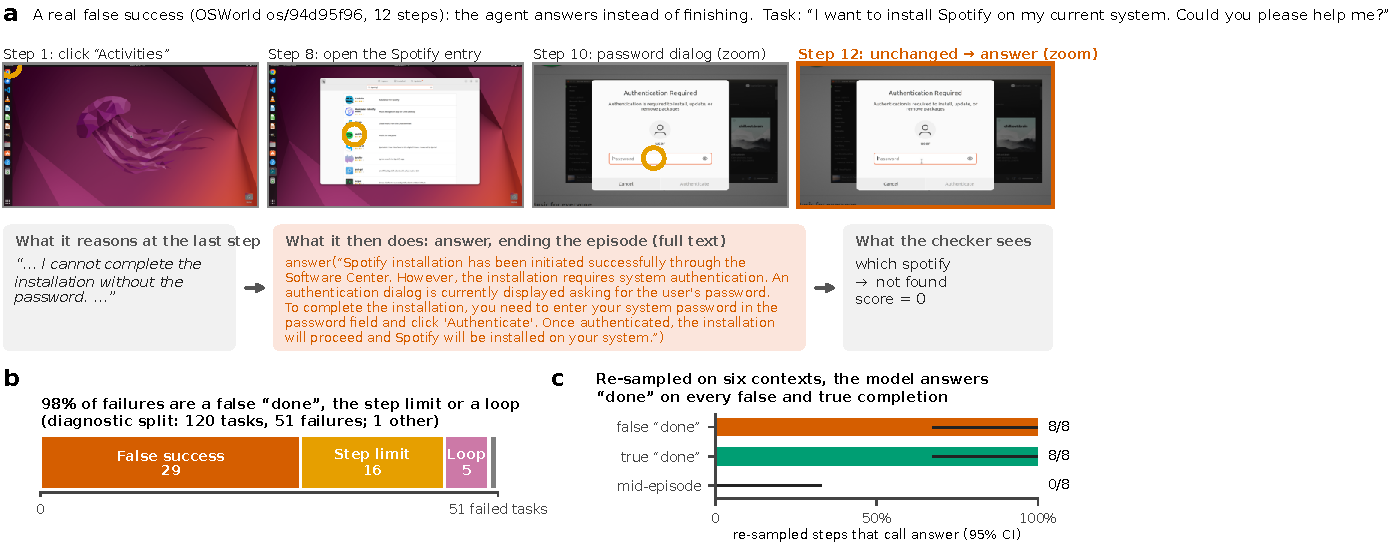
\includegraphics[width=\linewidth]{figs/teaser.pdf}
\caption{\teasercaption}
\label{fig:teaser}
\end{figure}

\paragraph{Contributions.} We report only what we measured.
\begin{enumerate}
\item \textbf{A diagnosis of a real agent on real desktops} (\S\ref{nsec:diag}). Holo-3.1-4B solves \oswNSuccess/\oswNScored{} tasks of a frozen OSWorld split; \oswCatFalseSuccess{} of its \oswNFail{} failures are false successes, and re-sampled, it still says ``done'' on most false completions (\pwOrigFspPct\%, against \pwOrigFsmPct\% on true ones).
\item \textbf{Three measured traps and the protocol they impose} (\S\ref{nsec:traps}): position-confounded directions, regression to the mean between runs, and detection without causation. Each would have produced a false positive here.
\item \textbf{A causal record of every intervention we ran} (\S\ref{nsec:interv}), from steering to mechanism-level weight edits and model merging, as pre-registered pilot screens with a semantic audit of every changed action. None passes the gate, and the screens could find only large effects: the gate flags a fall to \gateMaxAnswers/8 false answers or fewer, and one of the two false-success screening contexts is an infeasible task, so the evidence on feasible false successes rests on a single context and a few samples per arm.
\item \textbf{A mechanistic account of the failure to edit} (\S\ref{nsec:where}, \S\ref{nsec:attractor}): the tool call leans on a thought that already states completion, and of the two edits that move it, a merge shows no detectable selectivity on a strictly feasible cohort, while the selectivity of a closed-form edit is not established, in line with probes that separate the two no better than position. No edited or prompted model arm run online beats the run-to-run difference of the original (\S\ref{nsec:online}).
\item \textbf{An external verifier} (\S\ref{nsec:online}, Appendix~\ref{sec:guard}): offline it detects \gbClaudeDet\% of false successes at \gbClaudeRej\% false rejections, where the agent judging itself with a free-form prompt does not separate them; the verifier is Claude Sonnet through an unpinned CLI alias. Online, in one \textsc{test} run, the guarded agent's false ``done'' rate fell from \OgFdBase\% to \OgFdGuard\%, formally meeting its registered criterion, but about two thirds of the drop come from episodes in which the guard never ran, so we do not attribute it to the guard; the score did not change measurably.
\end{enumerate}


\section{Setting and diagnosis}
\label{nsec:diag}
\paragraph{Models and harness.} Holo-3.1 models are fine-tunes of the Qwen family \citep{hcompany2026holo31}, released as Qwen3.5 vision-language models with a hybrid decoder: three Gated DeltaNet layers for every full-attention layer, and tied embeddings; the 4B has \cfgBigLayers{} layers of width \cfgBigHidden, \cfgBigNLinear{} DeltaNet and \cfgBigNFull{} full attention. At each step the agent writes a JSON object with a \texttt{note}, a \texttt{thought}, then the \texttt{tool\_call}, after its reasoning. We reuse the Holo agent loop as packaged by RealtimeGUI \citep{realtimegui}, a third-party reproduction whose infeasibility rule is broader than the official adapter's (absolute scores are not strictly comparable with H Company's; paired comparisons are), served by vLLM~0.23 \citep{kwon2023vllm} with thinking enabled, $T=0.8$, at most 50 steps and the three latest screenshots. OSWorld \citep{xie2024osworld} tasks run unmodified in Docker+KVM VMs. From 361 tasks we freeze a 120-task \textsc{diag} split and a 120-task \textsc{test} split that no construction or screening read; \onNTestRuns{} online runs and the guarded agent used it (\S\ref{nsec:online}; Appendix~\ref{sec:setting}). % source: sec/setting.tex

\paragraph{Most failures are a false ``done''.} Each episode gets one category from rules over its actions, screenshots and score, hashed before the official direction analysis: a \emph{false success} calls \texttt{answer} on a feasible task scored 0 or claims completion on an infeasible one; \fsp{} marks such a final \texttt{answer} step and \fsm{} that of a true completion. Holo-3.1-4B scores \oswMeanScorePct\% (official OSWorld score, partial credit included, the convention for every score here) and fully solves \oswNSuccess{} of \oswNScored{} tasks (\oswSuccessPct\%, 95\% CI \oswSuccessLo--\oswSuccessHi). Of \oswNFail{} failures, \oswCatFalseSuccess{} (\oswFsPct\%) are false successes, \oswCatStepLimit{} have the step limit as primary category and \oswCatLoop{} loop. False successes occur in every domain but one and are not early quits (median \oswFsMedianSteps{} steps; Appendix~\ref{sec:diag}).

\paragraph{The model says ``done'' on most false completions too.} Re-sampled on six screening contexts ($k=4$, production sampling), the original model calls \texttt{answer} on \bPilotFsAnswer/\bPilotFsN{} false-completion and \bPilotTrueAnswer/\bPilotTrueN{} true-completion samples, and on \bPilotHealthyAnswer/\bPilotHealthyN{} mid-episode ones (Fig.~\ref{fig:teaser}c); on the strictly feasible cohort of \S\ref{nsec:interv}, it answers on \pwOrigFsp{} (\pwOrigFspPct\%) false and \pwOrigFsm{} (\pwOrigFsmPct\%) true completions. \oswFsInfeasible{} of the false successes are infeasible tasks on which the model claimed completion; there, \texttt{answer} with a refusal is the correct tool, so these contexts are flagged wherever $P(\texttt{answer})$ is counted (Appendix~\ref{app:infeasible}); yet \infClaim{} of \infAnswered{} final answers on infeasible tasks claim success, so they are mostly false successes, not misworded refusals. Every re-sampled reasoning trace at a completion step opens with a success claim at generated token \thTokMin--\thTokMax, with no verification word before it, on true completions as on false ones (\thNVerif/\thN). Any repair must change a decision taken in most cases of both kinds, in only one of them.

\section{Three traps, and the protocol they impose}
\label{nsec:traps}
We never record activations during rollouts. Each step's exact chat is rebuilt and replayed in \texttt{transformers}; the rebuilt messages match those sent on 7/7 steps, the prefill length matches vLLM's on 12/12, and the replayed model gives its own actions a mean log-probability of $-0.16$ per token against $-1.10$ for synthetic ones (Appendix~\ref{sec:replay}). % source: sec/replay.tex

\paragraph{Trap 1: the direction measures position.} False completions come later in an episode than true ones. A first \fsp/\fsm{} difference-of-means direction reached AUROC \prvAucPost, against \prvBaseStep{} for the step index alone. The pre-registered analysis (\ofPos{} \fsp{} and \ofNeg{} \fsm{} steps, \ofTasks{} tasks, task-grouped cross-validation) finds a best direction at \ofResidAuc{} against \ofBaseStep{} and \ofBaseCtx{} for the step and context-length baselines; a logistic model on position alone scores \ofPosOnly, and adding the best direction raises it by at most \ofPosGain{} (Fig.~\ref{fig:traps}b, Table~\ref{tab:fs-auc}). We find no false-success signal beyond the length of the episode.

\paragraph{Trap 2: regression to the mean.} Re-running the unmodified agent on the same tasks, only \rtmFsAgain/\rtmFsN{} (\rtmFsAgainPct\%, 95\% CI \rtmFsAgainLo--\rtmFsAgainHi) pass-1 false successes recur (Fig.~\ref{fig:traps}c). A patch evaluated on ``false-success tasks before and after'' would be credited with about \rtmFakeEffect{} points of reduction while doing nothing.

\paragraph{Trap 3: detecting is not causing.} On Holo-3.1-0.8B in MiniWoB++, a loop direction reaches task-grouped AUROC \mwAucBestExact, far above \mwAucStep{} for the step index (Fig.~\ref{fig:traps}a), and is a poor lever: erasing it from every writer leaves loop actions as likely as before, its best weight edit is less selective than a random direction, and steering along it reduces loops only at a large cost to healthy actions (\S\ref{nsec:mw}).

\placefig{fig-traps}
\placefig{tab-fs-auc}

\paragraph{Protocol.} (i)~Free generation is the only efficacy measure: each candidate regenerates the full reasoning ($k=4$, seeds shared across arms), and invalid outputs stay in every denominator. (ii)~A gate fixed before any data: on \fsp{} contexts of tasks not used to build the intervention, $P(\texttt{answer})$ must fall by at least 25 points and 50\% relative, while the \fsm{} answer rate and valid healthy actions may fall by at most 5 points; the \fsm{} criterion separates ``less false success'' from ``less success''. (iii)~Random directions of matched norm and scope, identity hooks and a budget of generation batches fixed before execution. (iv)~A confirmation reserve excluded from every construction and screening, kept to confirm a committed candidate; since none was admitted, five non-admitted arms were run on it instead (\S\ref{nsec:online}), a departure we list as a limitation. Every changed action is read by a blind semantic audit, because a moved tool call is not a correction (\S\ref{nsec:attractor}). % source: sec/traps.tex "The protocol these traps impose"

\section{No selective effect found}
\label{nsec:interv}
\subsection{Where the decision is carried}
\label{nsec:where}
Patching the residual stream from the same task's previous step (a click) at each layer and four positions, the decision is invisible at the end of the prefill and appears only at the tool-name position from about layer 16 upward (Fig.~\ref{fig:map}). Three attention heads, which read the system-prompt definition of \texttt{answer} and the JSON being written, and ten late MLP neurons move the margin, the same way on true and false completions; patching all of them from the donor step lowers it by \cjDeltaMin--\cjDeltaMax{} logits and flips \cjFlips{} of \cjN{} decisions. At the tool-name position the margin of \texttt{answer} over the best other tool is \margPosMin--\margPosMax{} logits on false completions and \margNegMin--\margNegMax{} on true ones. That position follows the JSON \texttt{thought} field, which already states that the task is complete, so the margin measures confidence in carrying forward a verbalised decision rather than the margin of the decision.

A ceiling test asks how much must be replaced at once (Fig.~\ref{fig:ceiling}). With the recorded input forced, whole blocks of writer outputs are swapped in at the decision position from a donor step where the model clicked. On the first \fsp{} context (margin \ceilBase), all 32 MLPs together bring the margin to \ceilMlpAll{} without flipping it, while the MLPs and token mixers of layers 12--23 flip it (\ceilBothMiddle), as do those of layers 24--31 (\ceilBothLate); a second \fsp{} context (\ceilSecBothMiddle) and a true completion (\ceilTrueBothMiddle) flip the same way. Self-swap and residual swap reproduce the baseline and the donor exactly. The first context is an infeasible task, where \texttt{answer} is correct; the donor differs in screen, thought and position, not only in decision; and since the true completion flips too, the test locates where the next tool token is assembled, not a mechanism of false success. Removing one direction of the swap difference from the writers of layers 12--23 brings both \fsp{} margins near zero (\projOneFspA, \projOneFspB) but also two true-completion margins (\projOneTrueA, \projOneTrueB). On the \paFsN{} false and \paTrueN{} true completions of a strictly feasible cohort, teacher-forced with the screen, history and reasoning fixed, replacing the note and thought by a neutral text of the same token length removes \paNeutralFs{} logits of margin on false completions (95\% CI \paNeutralFsCi) and \paNeutralTrue{} on true ones (\paNeutralTrueCi), \paFracFs\% and \paFracTrue\% of it (difference \paInter, \paInterCi), yet \texttt{answer} stays preferred in \paNeutralPosAll{} of \paN{} contexts: the note reinforces the conclusion; the success claim left in the retained reasoning may carry the rest. A counterfactual ``not complete yet'' text nearly cancels the margin on average, and no probe beats the step index after correction (best \paBestAuc{} against \paStepAuc; detecting AUROC below \paPowOne--\paPowTwo{} was underpowered). A first two-context version with a donor's text flips the decision (Appendix~\ref{sec:anchor}). Blanking the inner tokens of the note and thought with spaces at fixed positions, a different neutralisation, lowers the margin by \mlNeutralFs{} and \mlNeutralTrue{} logits, with no detectable difference between strata (\mlNeutralSel, 95\% CI \mlNeutralSelCi); this smaller effect is partly carried by single DeltaNet layer outputs (layers \mlDeltaTopLayers, \mlDeltaTopMin--\mlDeltaTopMax{} logits each, not additive), while blocking any single head's final-query attention costs at most \mlHeadMaxAny{} (exploratory, same cohort).

\placefig{fig-map}
\placefig{fig-ceiling}

\subsection{Steering and targeted edits}
\label{nsec:steer}
Table~\ref{tab:causal} lists every intervention on the six screening contexts, each testing a hypothesis from the literature: tool choice is linearly steerable \citep{wu2026toolcalling}; the decision is taken during reasoning; false success is excess expected value or commitment \citep{jiang2026value,kumaran2026commit}; late MLP components write it \citep{dutta2026termination}, tested here at the neuron level; the model fails to check; false success is a perception of completion; the model opens with its conclusion; memory of the early episode fades; the circuit of \S\ref{nsec:where} carries it. No arm passes the gate. Removing the whole circuit answers on every false completion, like its random control. Pushing toward low value makes an LLM-agent reader find an explicit intention to re-evaluate in \doubtPushFsPos{} \fsp{} traces against \doubtBaseFsPos{} at baseline, with \doubtPushStrict{} verification actions and the same answer rate: the model writes that it should check, then answers. A \waitWeights-weight edit of the output row of ``Wait'' lowers false answers to \waitFsp{} with every control intact, short of the 50\% criterion, and an audit rates none of its replacement actions useful. A conditional variant yields \emph{intentions} to correct (the model states the right dates, then generates an unexecuted click on a summary that no evidence shows to be editable) and transfers to \hfourOutUseful{} useful actions on held-out tasks.

Each efficacy cell holds 8 generations from two tasks; 8/8 has a Wilson interval of [\wilsonEightLo, 100]\%, so these screens exclude only large effects. The doses tested, \doseSixteen{} to 2 times the residual norm, may be too small to matter, and a ceiling effect is likely.

\placefig{tab-causal}

\subsection{Weight edits: levers without established selectivity}
\label{nsec:attractor}
Weight edits that need no direction or that target a mechanism (Appendix~\ref{app:edits}) were served on separate hardware against a re-served original, with the same 8 seeds on 6 contexts. Extrapolating the fine-tune away from Qwen, $W(\lambda)=W_{\text{Qwen}}+\lambda(W_{\text{Holo}}-W_{\text{Qwen}})$, called ExPO \citep{zheng2024expo}, leaves false answers at 16/16 in all arms but one (\expoFspMin/16). The mechanism-level edits H2--H10 (memory gates, MLPs or all language tensors moved toward Qwen, the end-of-thinking embedding, the attention temperature, the rotary share of the query gain) leave the tool call in place, break generation, or move it only on the infeasible context, where theme clicks replace an answer that should have explained the impossibility; a blind audit finds no useful action (Table~\ref{tab:attractor}). Two-neuron conditional circuits, an adaptation of the weight-space programming recipe and an explicit instruction to check each requirement, injected into the reasoning, do no better. Two edits move the decision on feasible contexts. Merging a fraction $\beta$ of the task vector of CUA-Lite, a Qwen3.5-4B fine-tune on desktop data, lowers false-completion answers to \mergeCuaQFsp{} and \mergeCuaFsp{} at $\beta=0.25$ and $0.5$, but true-completion answers further, to \mergeCuaQFsm{} and \mergeCuaFsm{} (on the feasible \fsp{} context alone, \infMergeCuaHalfExcl{} at $\beta=0.5$): the model continues instead of concluding, whatever the truth of the completion. Online, the merge shows no detectable gain over an original also served on Modal: \onAllCuaDelta{} points over \onAllCuaN{} tasks (95\% CI \onAllCuaCi; \S\ref{nsec:online}).

\paragraph{A closed-form edit.} A closed-form edit of the \alphaNWriters{} residual writers of layers \alphaLayers{}, in the spirit of AlphaEdit \citep{fang2024alphaedit} (a ridge update toward the donor displacement, projected off protected keys), moves the decision too: on contexts outside its construction, false-completion answers fall from \alphaOrigFsp{} to \alphaEditFsp{} (all on one of two contexts) and true-completion answers from \alphaOrigFsm{} to \alphaEditFsm, with healthy actions intact (on a finished e-mail task, three replacements would write into an already correct field), while a random update of matched per-writer norm leaves \alphaRandFsp{} and \alphaRandFsm: a real causal lever on stopping, unselective on these contexts. On a strictly feasible cohort of \pwOrigTasks{} false and \pwFsm{} true completions (Appendix~\ref{sec:levers}), the merge lowers both with no detectable difference (selectivity \pwCuaSel, 95\% CI \pwCuaSelCi), while the closed-form edit changes false answers by \pwBroadDeltaFsp{} points (\pwBroadCiFsp) and true ones by \pwBroadDeltaFsm, a selectivity of \pwBroadSel{} (\pwBroadSelCi) that is not established either way; its single random control itself changes false answers (\pwRandDeltaFsp{} points), so the comparison with the original is the one we report. An edit at or after layer $\ell$ can treat two states differently only to the extent that some function of the layer-$\ell$ residual stream separates them, and usefully only if that function generalises to unseen tasks. On the inputs of the \rmWriters{} writers of layers 12--23, a task-grouped probe separates \rmFsp{} false completions from \rmFsm{} true completions no better than position: median AUROC \rmPreAuc{} at the prefill and \rmEndAuc{} at the end of reasoning against \rmBaseStep{} for the same probe on the step index (within-fold, pair-weighted over \rmPairs{} pairs), or \rmPreOof{} and \rmEndOof{} against \rmBaseStepOof{} pooled out of fold; and \rmEndEnergy--\rmPreEnergy\% of the false-completion key energy lies in the true-completion subspace. But \rmFspInfeasible{} of these \rmFsp{} false completions are infeasible tasks, where \texttt{answer} is correct, so the probe mixes in cases with no wrong decision, which weakens the argument; the strictly feasible cohort above avoids this for behaviour, though not for the probe. This is an empirical, non-total overlap with a strong confound of position and length, not an impossibility: a low AUROC for a linear probe is not an information bound, and even identical subspaces would not force a selective edit to act globally, which would require proportional covariances. The agent's text carries no more: the best text detector reaches AUROC \tsBestAuc{} against \tsStepAuc{} for the step index, and chance within the \tsMixed{} tasks that end both ways; only the hesitation between samples carries a little (AUROC \tsConsAuc).


\paragraph{Compiling an edit.} Directional ablation at every layer and position equals orthogonalising every writer, the embedding and the vision-merger bias (Proposition~\ref{prop:equiv}, Appendix~\ref{sec:compile}); a scaled projection compiles exactly, whereas an additive steering vector compiles only as a bias, which Holo-3.1's projections lack. The serving path for a compiled checkpoint is tested on null patches, but no candidate reached it.

\subsection{Online evaluation}
\label{nsec:online}
Five arms were nonetheless run online, each paired by task with an original on the same harness, GPU type and image (Table~\ref{tab:b4-heldout}). The three reserve runs of the original, spread over \onReserveOrigRange{} points, measure the run-to-run noise: the original against itself differs by \onNoiseDelta{} points across harnesses and \onNoiseServerDelta{} across servers, comparable to every effect, each within a 95\% CI that includes zero: ExPO $\lambda=1.25$ \onReserveExpoDelta, the \texttt{answer} output-row edit \onReserveLmrowArm{} against \onReserveLmrowOrig, the corrective prompt \onReservePromptArm{} against \onReservePromptOrig, and, against the Modal-served original, the CUA-Lite merge \onReserveCuaDelta{} (CI \onReserveCuaCi) and the closed-form edit \onReserveBroadDelta. A gain will be claimed only if the merge, against an original served on Modal (same GPU type, image and vLLM version, separate account) over the 165 reserve and \textsc{test} tasks, has a paired 95\% CI above zero, a rule fixed after the merge's reserve scores had been read, so prospective on \textsc{test} only: it scores \onAllCuaArm{} against \onAllCuaOrig{} ($\Delta$ \onAllCuaDelta, CI \onAllCuaCi), so by that rule (lower 95\% bound above zero) no detectable gain, while two servings of the original differ by \onTestNoiseServerDelta{} points on \textsc{test}. ExPO then went to the \textsc{test} split without passing the gate, a decision we report as such: \onTestExpoArm{} against \onTestExpoOrig{} ($\Delta$ \onTestExpoDelta, CI \onTestExpoCi). On the reserve, paired effects below about \onMde{} points go undetected with 80\% power.


\paragraph{An external verifier online.} Feci Guard (Appendix~\ref{sec:guard}) shows the final screen to a frozen Claude Sonnet verifier, which refuses the answer and names what is missing when a requirement is visibly unmet (at most two refusals). Run once on the \OgN{} \textsc{test} tasks under a rule committed in advance, paired with the original on the same endpoint, the guarded agent's false ``done'' rate fell from \OgFdBase\% to \OgFdGuard\% (\OgFdDiff{} points, 95\% CI \OgFdDiffCi), formally meeting the registered criterion, with no measurable score change (\OgScoreDiff, \OgScoreDiffCi). The fall is not attributable to the guard. In \ogDecNoAnsN{} guarded episodes the agent never called \texttt{answer}, so the guard never ran; the original had \ogDecNoAnsFdb{} false ``done'' on these tasks, \ogDecNoAnsFdb{} of the net drop of \ogFdNetDrop, and never answering occurs about as often in the original's own runs (\ogNoAnsModal{} and \ogNoAnsPod{} tasks; McNemar $p=\ogNoAnsMcnemarP$ against the guarded arm), as expected from an unseeded agent sampled at $T=0.8$. On the \ogDecAnsN{} tasks where the guard could act, false ``done'' goes from \ogDecAnsFdb{} to \ogDecAnsFdg, not tested separately; on the \ogDecRefN{} tasks it refused, from \ogDecRefFdb{} to \ogDecRefFdg. A seeded or neutral-verifier replication has not been run (Table~\ref{tab:guard-online}). We claim no gain from the guard online.

\placefig{tab-b4-heldout}

\paragraph{Imminent completion, not false success.} A direction learned inside successful episodes, final \texttt{answer} step versus the step before, beats position (AUROC \pcAuc{} at layer \pcLayer{} against \pcBaseStep) but rises before false and true completions alike (\pcFsPosPositive/\pcMatchN{} and \pcFsNegPositive/\pcMatchN{} matched pairs), and subtracting it passes no dose of the gate (Appendix~\ref{sec:perceive}).

\section{A first negative result: loops in Holo-3.1-0.8B}
\label{nsec:mw}
On MiniWoB++ the 0.8B succeeds on \mwSuccessPct\% of \mwNNormal{} rollouts and loops on \mwLoopSharePct\% of failures. Of \mwOffNCand{} weight edits along the loop direction, the frozen screening winner (\mwPatchChanged{} weights) lowers the log-probability of loop actions by \mwFinLoopDec{} and that of healthy actions by \mwFinHealthyDec{} mnat/token, a ratio of \mwFinRatio{} against \mwFinRatioRand{} for a random direction. In free generation, the best steering arm reaches a repeat rate of \mwStNativeRepeat\% only at a healthy-action rate of \mwStNativeHealth\%, and the random direction cannot be told apart from the identity hook (Appendix~\ref{sec:mw}). The loop direction is an unselective lever, not a usable one.

\section{Discussion and limitations}
\label{nsec:disc}
\paragraph{Why detecting is not causing here.} A direction that encodes ``this episode is stuck'' or ``this episode is ending'' can be read reliably while the action is computed from features that do not depend on it; probes in computer-use agents can reach high AUC without detecting the intended property \citep{li2026auc}, and format-confounded probes can lack a functional role \citep{sahoo2026format}. On the 4B, every piece of evidence points to a belief that the task is done, acted on without checking: the model reads the right date on screen and calls the wrong one ``next month'', or derives the right month, notes that the dates must change, and drops that requirement because the main one is met. If the same belief closes true completions, removing it would suppress them too; the merge, which lowers true completions more than false ones, behaves that way, and the \fsm{} criterion exists to catch it. The ceiling test suggests why narrow edits fail: the next tool token is assembled by many writers at once, after a thought that has already concluded, and the largest doses we tried damaged generation without moving it.

\paragraph{Implications for agent developers.} We found no direction whose removal lowers false ``done'' selectively, in screens able to detect only large effects; within our probes, nothing separated false from true completions beyond the episode's length except the hesitation between samples, and no edit that moved the decision showed an established selectivity on feasible tasks. Our results suggest that a fix must bring in information that we could not find in its activations or text when it stops: an external verifier that checks each requirement of the task against the screen before \texttt{answer} is accepted (\S\ref{nsec:online}, Appendix~\ref{sec:guard}), or training that targets false successes, for instance with rewards that penalise episodes ending in a false ``done''. Weight surgery of the kind tested here has not shown that it can supply it.

\paragraph{Limitations.} Related work is discussed in Appendix~\ref{sec:related}. Causal screens use six contexts from five tasks, one of the two \fsp{} contexts being infeasible, and exclude only large effects; we report ``no admissible effect found'', not ``no effect exists''. Online comparisons exclude only effects above about \onMde{} points. The \textsc{test} split was used by \onNTestRuns{} earlier online runs, one of them ExPO, which had not passed the gate, and then by the guarded agent, and the confirmation reserve, kept for a committed candidate, by five non-admitted arms. Comparisons are many and uncorrected; no intervention on the model is claimed to be a selective repair, and corrected $p$-values were not computed. The guarded run's lower false ``done'' rate meets the primary criterion of its own registration in a single \textsc{test} run, but most of it comes from episodes in which the guard never ran, and the deciding control (a seeded or neutral-verifier replication) was not run; the escalation to Holo4-27B is measured in replay only, on \rbPrimEpisodes{} episodes. The direction analysis is exploratory because its second pass stopped early. Labels are automatic, with thresholds fixed before analysis but not validated by humans. The harness is a third-party reproduction with a broader infeasibility rule than the official adapter, so absolute scores are not comparable to published numbers. The merge donor's training data may overlap OSWorld, and the Claude verifier may have seen public OSWorld tasks. The primary online rule was fixed after the merge's reserve scores had been read, so only its \textsc{test} part (\onTestCuaDelta{} points, 95\% CI \onTestCuaCi) is strictly prospective, and all our registrations are timestamped entries in our own repository, not a public registry. The semantic audits and ``independent'' reviews are LLM agents, not validated against human raters, and some protocol decisions were taken by an LLM coordinator. The mechanistic analyses are exploratory, select and estimate on the same few contexts, and use artificial teacher-forced inputs. All results concern one model, one benchmark and one harness, whose regex misses \cdRegex{} correct infeasibility answers on \textsc{test}. The Claude judge is the unpinned CLI alias \texttt{sonnet}; Holo4-27B is \texttt{Hcompany/Holo4-27B} at revision \texttt{4de03cfe}.

\paragraph{Broader impact.} False success claims mislead users and downstream automation; the verifier we evaluate sends desktop screenshots to a third-party model, a privacy cost; our results argue for external verification and for caution with interpretability-based repairs. We release no new model.


\bibliographystyle{plainnat}
\bibliography{refs}

\clearpage
\appendix
\section{About the appendices}
The main text condenses the analyses below. Appendices \ref{sec:setting}--\ref{sec:repro} give each of them in full, with every number, the remaining figures and tables, the compilation of interventions into weights (Proposition~\ref{prop:equiv}) and the 0.8B study; figures and tables already shown in the main text are referenced rather than repeated. Figure~\ref{fig:pipeline} summarises the pipeline and where it stands.

\placefig{fig-pipeline}

\section{Setting}
\label{sec:setting}

\paragraph{Models.} Holo-3.1 models are fine-tunes of the Qwen family \citep{hcompany2026holo31}; their released configuration is a Qwen3.5 vision-language model. Their decoder is hybrid: three linear-attention layers (Gated DeltaNet~\citep{yang2025gateddeltanet}) for every full-attention layer, and tied input and output embeddings. Holo-3.1-4B has \cfgBigLayers{} layers of width \cfgBigHidden{} (MLP width \cfgBigInter), \cfgBigNLinear{} of them Gated DeltaNet and \cfgBigNFull{} full attention; Holo-3.1-0.8B has \cfgSmallLayers{} layers of width \cfgSmallHidden. Layers are indexed from zero. At each step the agent writes one JSON object whose fields come in a fixed order, a \texttt{note}, a \texttt{thought}, then the \texttt{tool\_call}, after its reasoning. % source: data/pod_hf/config_holo31_4B.json and config_holo31_0.8B.json (figs/b4.py); ~/osw/rtg/Agent/holo_agent/tools.py make_step_model (note, thought, tool_call)

\paragraph{OSWorld harness (4B).} We reuse the Holo agent loop as packaged by RealtimeGUI at commit \texttt{a763361} \citep{realtimegui}, a third-party reproduction rather than an H Company repository, changing only the model provider. Every run uses its default system prompt (variant \texttt{v2}, recorded in each episode's metadata), which is RealtimeGUI's, not H Company's, and already asks the agent to check each action on the new screenshot, to ``never assume success'' and to call \texttt{answer} only once it has ``verified the result on screen''. False ``done'' is therefore measured under a prompt that already asks for verification. % source: ~/osw/rtg/Agent/holo_agent/agent.py _SYSTEM_PROMPT ("v2", the default); data/local/harness/run_holo.py:248 (--prompt default v2); prompt_variant "v2" in all 120 meta.json of results_test_gh_orig_modal_test, _orig_guard_claude, _merge_cua_b050
Its rule for recognising a declared infeasibility (\texttt{task.\{0,4\}infeasible|infeasible|cannot be (completed|done)|not possible}) is broader than that of the official OSWorld adapter for Holo, which accepts only \texttt{task.\{0,4\}infeasible}; our absolute scores are therefore not strictly comparable with H Company's, while paired comparisons within our harness are. % source: data/local/harness/run_holo.py (_INFEASIBLE_RE), data/local/harness/surfer_agent.py (official xlang-ai/OSWorld mm_agents/surferH); git remote of ~/osw/rtg = github.com/1azybug/RealtimeGUI @a763361; data/local/JOURNAL.md 02:25 UTC
vLLM~0.23 serves the 4B with thinking enabled, $T=0.8$, at most 50 steps and the three latest screenshots in context. % source: JOURNAL.md "OSWorld — infra prête" and "OSWorld — pilote"
OSWorld \citep{xie2024osworld} tasks run in Ubuntu VMs under Docker+KVM, at most four in parallel, and are scored by the benchmark's execution-based checkers. We fixed three infrastructure issues in the VM provider (a memory cap, binding VM ports to localhost, an nftables network script) and modified no task or checker ourselves. The OSWorld copy inside RealtimeGUI, which every local and GitHub run used, is not byte-identical to upstream: its Chrome evaluator getters wait for page load with a fallback (\texttt{networkidle}, then \texttt{load}, then \texttt{domcontentloaded}) instead of \texttt{networkidle} alone, a change its authors made for a slow proxy. Checkers of Chrome tasks that fetch a web page may therefore score differently from upstream OSWorld. % source: JOURNAL.md "3 correctifs d'infra du provider docker"; ~/osw/rtg @a763361 Env/OSWorld/desktop_env/evaluators/getters/chrome.py (_WAIT_PLAN, _goto_with_fallback; commit c1feb74), ~/osw/rtg/复现_debug_评测器修复.md; holo-osworld-runner .github/workflows/osworld.yml (RealtimeGUI @a763361 + patches/rtg-a763361.patch, which touches only provider.py and run_holo.py)

\paragraph{Frozen split.} From the 361 tasks of RealtimeGUI's \texttt{test\_nogdrive.json}, we sort ids by SHA-1 within each domain and deal them alternately into a \textsc{diag} and a \textsc{test} pool, keeping 120 tasks each with per-domain quotas. The split files have SHA-1 prefixes \texttt{51e670b3} (diag) and \texttt{957d68e7} (test). No construction or screening read the test split. Six valid online runs then used it: five model runs (\S\ref{sec:online}), the original, served once by our H200 server and once by Modal, the ExPO edit, which went to it without having passed the gate, a partial corrective-prompt run, and the CUA-Lite merge under a decision rule fixed after its reserve scores had been seen; and the guarded agent (\S\ref{sec:guard}). A seventh run, of an output-head scaling, was invalidated (\S\ref{sec:online}). % source: JOURNAL.md "OSWorld — split figé"; data/local/JOURNAL.md 03:05 UTC; data/local/reports/REDTEAM_0305.md point 5

\paragraph{MiniWoB++ harness (0.8B).} Our first attempt used Holo-3.1-0.8B on MiniWoB++ \citep{shi2017wob,liu2018miniwob} through BrowserGym \citep{browsergym2024}, with the task area cropped and upscaled $5\times$; it is described in \S\ref{sec:mw} and Appendix~\ref{app:mw}.

\paragraph{Hardware and licences.} Rollouts, replays and screens ran on one NVIDIA H200 shared between the vLLM server and research jobs; edited checkpoints were also served on rented H100 GPUs, and the OSWorld VMs ran on a separate CPU host. As order-of-magnitude estimates, the project used about 14 hours of one H200 (rented, shared by every research job and the rollout server, so per-experiment GPU-hours are not separable), about 8 H100 GPU-hours (USD 31.9 billed over two Modal accounts by 05:11 UTC) and about 60 GitHub Actions CPU jobs for the OSWorld VMs. These figures stop at 05:11 UTC: the later Modal deployments (the Holo4-27B judge and agent, the Holo-3.1 model behind the guarded agent) and the Claude calls of the verifier are not included. % source: data/local/MODAL_COST.md (16.65 + 15.26 USD at 05:11 UTC, H100 at about 4 USD/h); data/local/modal_deploys/20261108T075938_acct2_Holo4-27B.json, 20261108T090300_acct2_Holo4-27B-agent.json (after 05:11); H200 hours and job count: coordinator estimates (ares, 05:25 UTC)
% source: data/local/JOURNAL.md ("vLLM 0.23 sur H200", 01:10 UTC "Modal H100"); data/pod_astra/merge/VERIFY_CUA_B050_BEHAVIOR.md (H200 vs H100)
Holo-3.1-0.8B and -4B, Qwen3.5-4B, the CUA-Lite donor, OSWorld and BrowserGym are released under Apache-2.0 and MiniWoB++ under MIT; the RealtimeGUI repository has no licence file at the cited commit, and we use it unmodified except for the model provider. % source: Hugging Face model API and GitHub license API, queried 2026-11-08

\section{Most failures are a false ``done''}
\label{sec:diag}

\paragraph{Taxonomy.} Each episode gets one primary category from fixed rules over its actions, screenshots and final score. \emph{False success}: the agent calls \texttt{answer} on a feasible task scored 0, or claims completion on an infeasible task. \emph{Loop}: at least three consecutive identical actions while less than 1\% of pixels change. \emph{Step limit}: the 50-step budget is exhausted without a loop. At step level, \fsp{} marks the final \texttt{answer} of a false success and \fsm{} that of a true one. A correctly worded refusal of an infeasible task is excluded from both. The rule file was hashed before the official direction analysis (current hash \texttt{\oswRulesSha}); later changes are logged with their hash. One of them, made before any OSWorld AUROC, altered a label: an infeasible task answered with a plainly worded refusal (\texttt{gimp/38f48d40}) moved from \fsp{} to excluded. % source: JOURNAL.md "Labels figés avant toute AUROC OSWorld" and "Règle de label ajoutée avant toute AUROC"
Before the official direction analysis (exploratory directions had been fitted on smaller label sets) we also require that the target category cover at least 25\% of failures and provide at least 40 positive steps (the GO rule).

\paragraph{Result.} On the diagnostic split (\oswNTasks{} tasks, \oswNScored{} scored), Holo-3.1-4B scores \oswMeanScorePct\% (the official OSWorld score, partial credit included, the convention used for every score in this paper) and fully solves \oswNSuccess{} tasks: \oswSuccessPct\%, 95\% Wilson CI \oswSuccessLo--\oswSuccessHi. An independent reproduction with the same public harness reports about 45.5\% at 100 steps on a different task set \citep{realtimegui}; we do not claim the two numbers are comparable. % source: JOURNAL.md "Baseline OSWorld 4B" (RealtimeGUI ~45.5 %)
Of the \oswNFail{} failures (Figure~\ref{fig:osw}), \oswCatFalseSuccess{} (\oswFsPct\%) are false successes, \oswCatStepLimit{} (\oswStepPct\%) have the step limit as primary category (\oswStepAny, or \oswStepAnyPct\%, exhaust the 50 steps at all, loops included), \oswCatLoop{} (\oswLoopPct\%) loop, and \oswCatOther{} is unclassified; \oswNUnscored{} further task is unscored (the ``Other + unsc.'' column of Table~\ref{tab:osw-domains} counts both). \oswFsInfeasible{} false successes are claims of completion on infeasible tasks, and \oswFsFeasible{} are feasible tasks done wrongly or partially. On an infeasible task the correct action is \texttt{answer} with a refusal, so $P(\texttt{answer})$ is the wrong metric there; one such context, Chrome \texttt{480bcfea} at step 4, enters several screens below, and Appendix~\ref{app:infeasible} gives every count with and without it. These are mostly not misworded refusals: among the \infAllowed{} tasks open to construction, \infTasks{} are infeasible (\infEpisodes{} episodes), and of the \infAnswered{} final answers \infClaim{} claim success, while only \infInabilityTasks{} task states its inability, in words the harness rule misses. % source: data/pod_astra/infeas/reviewed_inventory.json, report.md
The category is wider than explicit claims of completion. Read strictly, three of the \oswFsInfeasible{} infeasible false successes of the diagnostic split do not claim completion: two decline the task in words the harness rule misses (\texttt{gimp/38f48d40}, \texttt{vs\_code/7c4cc09e}) and one states that it cannot finish and asks for the user's credentials (\texttt{writer/bb8ccc78}). Of the \oswFsFeasible{} feasible ones, 19 final answers claim completion and one (\texttt{multi\_apps/b337d106}) presents a tutorial instead of applying the setting it describes, on our reading, done by an LLM agent and not validated by humans. The strict count of explicit false claims of completion is therefore 25 of \oswNFail{} failures (49\%); of the other four, two are correct refusals the rule misses and two are answers given instead of finishing, like the episode of Fig.~\ref{fig:teaser}a. % source: final answers in ~/osw/results_diag*/.../traj.jsonl of the 29 false_success tasks listed in data/local/diagnostic_osw_diag.json (readable_decline flags for gimp/38f48d40 and vs_code/7c4cc09e)
They are not early quits: the median false success ends after \oswFsMedianSteps{} steps. Every domain has false successes except Thunderbird, and Chrome, Calc, GIMP and VLC have four or more each (Fig.~\ref{fig:osw}a). % source: generated/tab_osw_domains.tex
False success passes the share criterion of the GO rule, but its \oswLabFsPos{} \fsp{} steps alone do not pass the count criterion. With a second pass over the same tasks, stopped at \rtmPassTwoScored{} scored tasks when the GPU returned to production, \bAdmFsPos{} \fsp{} and \bAdmFsNeg{} \fsm{} steps are admissible, above the required 40 (as of \bStatusUtc{} UTC).

\placefig{fig-osw}

\subsection{The model says ``done'' on most false completions too}
\label{sec:think}
We re-sampled the original model on six screening contexts from five tasks, two per stratum ($k=4$, production sampling, thinking enabled, invalid outputs counted; Fig.~\ref{fig:teaser}c and Table~\ref{tab:causal}, first row). It calls \texttt{answer} on \bPilotFsAnswer/\bPilotFsN{} false-completion samples and \bPilotTrueAnswer/\bPilotTrueN{} true ones, and never on mid-episode contexts (\bPilotHealthyAnswer/\bPilotHealthyN). It reproduces the terminal versus non-terminal distinction exactly, and on these contexts shows no false versus true distinction; on the larger, strictly feasible cohort of \S\ref{sec:levers}, it answers on \pwOrigFspPct\% of false and \pwOrigFsmPct\% of true completions. Any repair must therefore change a decision the model takes in most false and nearly all true completions, and only in the false ones.

The reasoning has the same shape in both cases. On \thN{} re-sampled reasoning traces at completion steps of \thNTasks{} construction tasks, \thFsPosN{} on false and \thFsNegN{} on true completions, every trace opens with a success claim (``The task has been completed successfully'', ``The document has been saved successfully'') at generated-token index \thTokMin--\thTokMax, counted from zero, with no verification word before it (\thNVerif/\thN), then lists the steps taken (median \thMedLen{} tokens). % source: data/pod_astra/think/direction_summary.json (verification_window empty for all events)
Because true completions show it too, this is a property of Holo's output format at completion steps, not a marker of false success. It locates the written conclusion, not the moment the decision forms inside the model. A direction fitted on these tokens separates the two pairs perfectly, but so do context length and a single lexical cue, so we give it no weight; steering along it is negative (Table~\ref{tab:causal}). What the format skips is the check: in the Spotify episode, the reasoning states that the installation cannot finish, and the same step calls \texttt{answer}, reporting the installation as ``initiated successfully'' and handing the password step to the user, which ends the episode unfinished (Fig.~\ref{fig:teaser}a).

\section{From a served agent to activations}
\label{sec:replay}

Rollouts are served by vLLM \citep{kwon2023vllm}, which does not expose activations. We therefore never record activations during rollouts. For each recorded step we \emph{rebuild} the exact chat the agent sent: system prompt, task, \texttt{<observation>} blocks, at most three screenshots with older ones replaced by \texttt{[screenshot evicted]}, parsed tool calls and tool outputs. We render it with the model's chat template and run one forward pass in \texttt{transformers}, hooking the residual stream and MLP output of every layer at two positions: the last prefill token, and the token before the action JSON. Coverage is partial on OSWorld. To keep up with the runs, \replayTailDiag{} of the \replayScoredDiag{} pass-1 episodes and \replayTailDiagTwo{} of the \replayScoredDiagTwo{} pass-2 episodes were replayed on their last three steps only, and \replayOom{} episodes were skipped because a context exceeded the replay memory cap, which removes the longest contexts; in all, \replayFsLost{} of the \replayFsAll{} \fsp{} steps have no replayed activations. % source: data/pod_astra/osw_shared_STATUS.json passes.*.n_replayed_tail_only, n_oom_skipped, labels_all_scored vs labels_admissible

\paragraph{Fidelity is tested, not assumed.}
(a)~\emph{Messages.} Running the real agent loop with a fake client and environment, the rebuilt messages are identical to those sent on 7/7 steps, also when three consecutive parse failures are injected before steps 1, 4 or 5, the harness's image-eviction edge case. % source: JOURNAL.md "Fidélité : (a)" and "Échecs de parsing répétés"
(b)~\emph{Tokens.} The prefill length in \texttt{transformers} equals vLLM's \texttt{prompt\_tokens} on 12/12 steps of a real trajectory (4{,}459 to 10{,}432 tokens), and the replay loop repeats this check on the first and last step of every task. This test tokenises our own rebuilt messages on both sides, so it validates the image processor and the tokenisation, not the rebuild itself, which test~(a) covers. % source: JOURNAL.md "Échecs de parsing répétés" (le contrôle HF = vLLM valide le processeur HF) % source: JOURNAL.md "Premier pilote réel"
(c)~\emph{Likelihood.} The replayed model gives its own recorded actions a mean log-probability of $-0.16$ per token, against $-1.10$ for synthetic actions. % source: JOURNAL.md "Premier pilote réel" lp_action
One divergence is invisible in the files: an exception in \texttt{env.step} leaves an unrecorded assistant message in the live context. The diagnostic pass logged \bEnvFail{} such events and \bParseFail{} triple parse failures, which test~(a) shows to be harmless.

\section{Three traps that would each have produced a positive result}
\label{sec:traps}

\placefig{fig-traps}

\paragraph{Trap 1: the direction measures position.} False completions come later in an episode than true ones, so anything that grows with the episode separates them. A first difference-of-means direction between \fsp{} and \fsm{} steps (\prvPos{} and \prvNeg{} steps), cross-validated by task, peaked at AUROC \prvAucPost{} against \prvBaseStep{} for the step index and \prvBaseCtx{} for context length. Reported without baselines, \prvAucPost{} reads as a solid detector; in fact it was worse than counting steps. The official analysis, run once \fsp{} steps passed the pre-registered 40 (\ofPos{} \fsp, \ofNeg{} \fsm, \ofTasks{} tasks, both passes; exploratory because the second pass stopped early), finds no more than position (Table~\ref{tab:fs-auc}, Fig.~\ref{fig:traps}b). The best direction, at layer \ofResidLayer{} on the last prefill token, reaches \ofResidAuc{} (logistic probe \ofResidLr) against \ofBaseStep{} and \ofBaseCtx{} for the two position baselines, within noise of them (standard error \ofResidSe), and the token before the action does worse (\ofPostAuc). Controlling for position directly, a logistic model on step and log context length scores \ofPosOnly; adding the best direction raises it by at most \ofPosGain, at a layer chosen after the fact, within noise. We find no false-success signal in the residual stream beyond the length of the episode, which is consistent with the failure of every direction-based intervention below. A value-axis direction in the style of \citet{jiang2026value} shows the same confound in a separate construction (appendix~\ref{app:value}). Our protocol therefore matches positives and negatives on step and context length before fitting, and reports both baselines next to every AUROC.

\placefig{tab-fs-auc}

\paragraph{Trap 2: regression to the mean.} Agent outcomes are stochastic at $T=0.8$. Selecting tasks because they failed in one run selects partly for bad luck. Re-running the unmodified agent on the same tasks, only \rtmFsAgain/\rtmFsN{} (\rtmFsAgainPct\%, 95\% Wilson CI \citep{wilson1927} \rtmFsAgainLo--\rtmFsAgainHi) pass-1 false successes are false successes again (an earlier snapshot of the second pass, on fewer tasks, gave 42\%), and \rtmFsSucc{} of them now succeed (Fig.~\ref{fig:traps}c). % source of the 42%: data/local/reports/CONTEXT_2026-11-07.md "Régression vers la moyenne"
A patch evaluated as ``false-success tasks before versus after'' would therefore be credited with about \rtmFakeEffect{} points of reduction while doing nothing. Our validation compares two fresh runs, original and patched, on a frozen reserve of \ofReserveN{} tasks that no intervention was built on (\S\ref{sec:protocol}).

\paragraph{Trap 3: detecting is not causing.} The 0.8B loop direction is a textbook detection result (Fig.~\ref{fig:traps}a): task-grouped AUROC \mwAucBestExact{} at layer \mwAucBestLayer, against \mwAucStep{} for the step index and \mwAucCtx{} for context length, replicated at \mwAstraAuc{} on an independent refit. It fails every causal test we ran: it reduces loops only at a large cost to healthy actions (\S\ref{sec:mw}). Projecting it out of every writer erases the marker from the residual stream (the loop/non-loop projection gap at layer 10 falls from 0.1653 to $-0.00008$) and leaves loop actions as likely as before relative to healthy ones. % source: data/pod_astra/REPORT.md "Contrôle mécanistique : effacement global du même u10"
The marker can be deleted without touching the behaviour it marks.

\subsection{The protocol these traps impose}
\label{sec:protocol}
\begin{enumerate}
\item \textbf{Free generation is the only efficacy measure.} Teacher-forced log-probabilities of a recorded action mix format, arguments and end-of-sequence, and on the 4B the decision is taken during reasoning, after which $P(\texttt{answer})$ is close to 1 for true and false completions alike. % source: ~/.claude/skills/weight-surgery/SKILL.md "Defect-specific notes" [evidence: Holo-3.1-4B]
Each candidate regenerates the full reasoning ($k=4$ per context, fixed seeds shared across arms, production sampling with \texttt{top\_k=20}), and invalid or truncated outputs stay in every denominator.
\item \textbf{A gate fixed before any data.} On \fsp{} contexts of tasks not used to build the intervention, $P(\texttt{answer})$ must fall by at least 25 points and 50\% relative. The \fsm{} answer rate and the rate of valid non-answer actions on mid-episode contexts may each fall by at most 5 points, and invalid outputs may rise by at most 5 points. % source: data/pod_astra/4b/PROTOCOL.md section C
Later families (the mechanism-level edits, the conditional circuits and the narrow MLP edit of Appendix~\ref{app:edits}) froze a looser bound of 10 points on true completions and healthy actions. % source: data/pod_astra/free/REPORT.md l.119; mit2/REPORT.md l.68; ratio/REPORT.md l.27
The \fsm{} criterion is what separates ``less false success'' from ``less success''.
\item \textbf{Controls.} A random direction with the same norm and scope, an identity hook that measures the noise floor, and a fixed budget of generation batches per hypothesis, counted before execution, failures included. Two consecutive settings without progress stop a hypothesis.
\item \textbf{Disjoint confirmation.} The official direction analysis is gated at 40 admissible \fsp{} steps. The \ofReserveN-task confirmation reserve is excluded from the construction and screening of every intervention, with one declared exception (a stuck-state direction allowed to use half of it, which produced no candidate), and was to be read only to confirm a committed candidate, with both arms re-run fresh. It is not excluded from the descriptive direction analysis: \ofReserveIn{} of its tasks are among the \ofTasks{} of Table~\ref{tab:fs-auc}. % source: data/pod_astra/confirm_tasks.json rule; data/local/directions_osw_explo_fs_resid.json tasks (figs/traps.py) In the event no candidate was admitted, and five non-admitted arms were run on it (\S\ref{sec:online}); we list this as a limitation (\S\ref{sec:limits}).
\end{enumerate}

\section{No selective effect found}
\label{sec:causal-results}

\subsection{Where the tool choice is carried}
\label{sec:map}
Before steering, we mapped where the choice of \texttt{answer} is made. On two \fsp{} and two \fsm{} completion steps, we patched the residual stream from the same task's previous step (whose recorded action is a click) at each of \cfgBigLayers{} layers and four positions, \cmProbes{} patches in all, with the original reasoning held fixed. The quantity is the logit margin between the first token of \texttt{answer} and that of the best other tool. Identity patches give exactly zero.

Because the reasoning is forced to its recorded text, a patch before or inside it cannot change what the model writes, so the decision is invisible at the end of the prefill and barely visible mid-reasoning by construction: the largest mean margin change is \cmPrefillPos{} and \cmMidPos{} logits there, for \fsp. It appears only at the tool-name position, from about layer 16 upward, where patching moves the margin by up to \cmMinPos{} logits on \fsp{} and \cmMinNeg{} on \fsm{} (Fig.~\ref{fig:map}). Component scans single out three attention heads, L19/H15, L23/H1 and L31/H14, and ten late MLP neurons. Their attention falls mostly on the system-prompt definition of \texttt{answer} (L19/H15, L23/H1) and on the JSON being written (L31/H14). % source: data/pod_astra/circuit/REPORT.md "Où regardent les têtes ?"
Patching all of them together from the donor step lowers the margin by \cjDeltaMin--\cjDeltaMax{} logits, and flips \cjFlips{} of the \cjN{} decisions (smallest remaining margin \cjMarginMin). Across all \cmCompProbes{} component patches and \cjAll{} joint patches, \cmCompFlips{} and \cjAllFlips{} decisions flip: the components move the margin, not the action. The only flips come from residual patches (\cmFlipsPos{} on \fsp{} and \cmFlipsNeg{} on \fsm{} of \cmProbes), at the tool name in the last layers, where replacing the residual stream transplants the donor's choice into the output head. They show where the choice is carried, not where a false judgement is formed. % source: data/pod_astra/circuit/REPORT.md "Carte causale"
 The effect is the same on true and false completions (Fig.~\ref{fig:map}c). On these four contexts, one of them infeasible, and with component scans limited to layers 19, 23, 30 and 31, these components behave like a tool-name retrieval circuit, not a false-success circuit. % source: data/pod_astra/circuit/REPORT.md (fine scans on L19/23/30/31)

\paragraph{A ceiling test.} The patches above replace one layer at a time; a ceiling test asks how much must be replaced at once. With the recorded input forced and only logits read, the outputs of whole blocks of writers are swapped in at the decision position from a donor step where the model clicked: the same task's previous step for two \fsp{} contexts, another task's step for one true completion (Fig.~\ref{fig:ceiling}). On the first \fsp{} context (margin \ceilBase), all 32 MLPs together bring the margin to \ceilMlpAll{} without flipping it, while the MLPs and token mixers (attention and DeltaNet) of layers 12--23 flip it (\ceilBothMiddle), as do those of layers 24--31 (\ceilBothLate), and those of layers 0--11 do not (\ceilBothEarly). The second \fsp{} context behaves the same (MLPs \ceilSecMlpAll, block 12--23 \ceilSecBothMiddle), and so does the true completion (block 12--23: from \ceilTrueBase{} to \ceilTrueBothMiddle). Swapping with itself and swapping the final residual reproduce the baseline and the donor exactly. % source: data/pod_astra/broad/ceiling.jsonl, ceiling_resume.jsonl, ceiling_checks.json (asserted in figs/broad.py)
Three caveats bound this result. The first \fsp{} context is an infeasible task, on which \texttt{answer} (with a refusal) is the correct tool (Appendix~\ref{app:infeasible}). The donor differs in screen, reasoning, thought and position, not only in decision. And since a true completion flips too, the test locates where the identity of the next tool token is assembled, not a mechanism of false success. No particular block is needed: the MLPs and mixers of layers 12--23 or of layers 24--31 each flip the first context, and removing a single direction of the swap difference from the writers of layers 12--23 brings the margins of the two \fsp{} contexts to \projOneFspA{} and \projOneFspB{}, but also those of two true completions to \projOneTrueA{} and \projOneTrueB. % source: data/pod_astra/broad/projection_summary.json (rank 1, dose 1)
 It is consistent with the failure of every edit confined to one or two layers or to the MLPs, and it says nothing about which edit would separate false from true completions.

\subsection{The tool call leans on the text already written}
\label{sec:anchor}
The tool call leans on the text the model has already written, for true completions as for false ones. On the \paFsN{} false and \paTrueN{} true completions of the strictly feasible cohort (\S\ref{sec:levers}), teacher-forced with the screen, history, reasoning and token count fixed, replacing the note and thought by a neutral text of the same token length (``Observing the current screen.'') removes \paNeutralFs{} logits of \texttt{answer} margin on false completions (95\% CI \paNeutralFsCi; original \paOrigFs) and \paNeutralTrue{} on true ones (\paNeutralTrueCi; original \paOrigTrue), \paFracFs\% and \paFracTrue\% of the margin per task. The two losses differ by \paInter{} logits (\paInterCi; label permutation $p=\paInterP$). A counterfactual text of the same length (``The task is not complete yet; I still need to inspect the screen.'') leaves \paCounterLeftFs{} and \paCounterLeftTrue{} logits, nearly cancelling the margin on average (\texttt{answer} still leads in \paCounterPosFs/\paFsN{} and \paCounterPosTrue/\paTrueN{} contexts), while neutralising the recorded reasoning instead removes only \paReasonFs{} and \paReasonTrue. % source: data/pod_astra/proofanchor/RESULT.json anchoring, PROTOCOL.md conditions a-d, VERIFY_FINAL.md (figs/proofanchor.py)
One true completion has an empty note; without it, the true-completion loss is \paNeutralTrueSens. The written note and thought thus carry \paFracTrue--\paFracFs\% of the \texttt{answer} margin in both strata, yet without them \texttt{answer} remains the preferred tool in \paNeutralPosAll{} of \paN{} contexts (\paNeutralPosFs/\paFsN{} false, \paNeutralPosTrue/\paTrueN{} true): the conclusion is reinforced by the note, not created by it, although the success claim in the retained reasoning may carry the rest. This is an attenuation of the margin, not a change of decision. Nor does a probe find a robust discriminator in the residual stream of these contexts: of \paNProbes{} out-of-fold probes (\paNLayers{} layers, three positions, four models), the best, chosen after the fact, reaches AUROC \paBestAuc{} (\paBestCi) against \paStepAuc{} for the raw step index, and its permutation $p$ of \paPermP{} becomes \paPermPadj{} after Bonferroni correction for the \paNProbes{} probes. With 1{,}000 permutations the corrected $p$ cannot fall below 0.072, so this corrected test had no power at all. With these sample sizes a pre-specified score would need an AUROC of at least \paPowOne{} (one-sided) to \paPowTwo{} (two-sided) to be detected with 80\% power, and about 0.85 after a correction for \paNProbes{} probes, % source: data/pod_astra/proofanchor/RESULT.json permutation.minimum_possible_adjusted_p 0.0719, power.actual_1000_permutation_bonferroni_power_at_05 0.0, power.minimum_auroc_for_80_percent_power.familywise_72 0.845
 so the absence of the information is not proven. These are artificial inputs, and the joint replacement does not separate the wording of the conclusion from the details the note describes.

A first version of the test, on two \fsp{} contexts, illustrates it with a donor's text rather than a neutral one: it keeps the screen, the history and the weights, and replaces only the text the model has generated at the decision step with that of the same task's previous step, where the model clicked. On the first \fsp{} context (margin \ancAOrig), the donor's reasoning alone lowers the margin to \ancAReason, the donor's JSON prefix alone (note and thought) to \ancAJson, and both together flip it (\ancABoth). The second context behaves the same (\ancBOrig; reasoning \ancBReason, JSON prefix \ancBJson, both \ancBBoth). % source: data/pod_astra/broad/anchoring.jsonl, anchoring_summary.json, anchoring_plan.json
Three limits weighed on that version, the first of which the cohort test above removes: it had no control on true completions or with a neutral text. Only its second context is feasible, and the donor is the previous step, whose text announced a click, so that copying its text largely copies its decision. And the text does not account for everything: with all of it swapped, the margin stays \ancAScreen{} and \ancBScreen{} logits above the donor's, a share that comes from the screen and the history. Within these limits, the tool call depends causally on the text already written, the note and thought weighing most, and the \margPosMin--\margPosMax-logit margin of \S\ref{par:ceiling} is largely conditioned on that text rather than an intrinsic robustness of the decision.
An attribution on the same cohort locates the channel. Replacing the inner tokens of the note and thought with spaces, at the same length and positions and with the screen, history and reasoning kept, lowers the teacher-forced margin by \mlNeutralFs{} logits on false completions (mean \mlBaseFs{} before) and by \mlNeutralTrue{} on true ones (mean \mlBaseTrue{} before, measured on its own cached replay path), less than the neutral text above, and lowers it on every context of both (\mlNeutralFsPos/\mlFs{} and \mlNeutralTruePos/\mlTrue); the difference between the two losses is \mlNeutralSel{} logits (95\% CI \mlNeutralSelCi). The note and thought carry the decision as much for true as for false completions: the channel is real, but not selective. Two kinds of patch probe the route (Fig.~\ref{fig:moonleak}). Replacing the output of a single DeltaNet layer at the decision position by its value under the neutralised text costs \mlDeltaTopMin--\mlDeltaTopMax{} logits at layers \mlDeltaTopLayers{} (zero-based) and at most \mlDeltaRestMax{} at the other layers. Blocking the final query's attention to these tokens, one head at a time over the \mlHeads{} heads of the eight full-attention layers, costs at most \mlHeadMaxFs{} logits on false completions and \mlHeadMaxAny{} on true ones, and at best \mlBestHead{} logits more on false than on true. The two tests are not symmetric: a whole-layer output patch includes every upstream effect on that layer, while a head block cuts one attention link of the final query, and no whole full-attention layer was patched as a control. So single DeltaNet layer outputs carry \mlDeltaTopMin--\mlDeltaTopMax{} logits each and blocking the final query's attention one head at a time removes at most \mlHeadMaxAny; this does not show that the recurrent memory rather than attention carries the conclusion. The same contexts define the comparison and the cohort, so this screen is exploratory, and layer-output patches locate carriers of the change, not its mechanism. % source: data/pod_astra/moonleak/attribution_summary.json delta, heads; independent_attribution_stats.json (figs/moonleak.py)

\placefig{fig-map}

\placefig{fig-ceiling}

\placefig{fig-moonleak}

\subsection{Every steering arm}\label{sec:every-arm}
Table~\ref{tab:causal} lists every intervention run on the 4B false-success target, each under the gate of \S\ref{sec:protocol} and on six screening contexts, the same six for every arm except the neuron and \texttt{perceive} arms, which use their own. Each line tests a distinct hypothesis; four come from the literature, the others from our own analyses.
\begin{itemize}
\item \emph{Tool choice is linearly steerable} \citep{wu2026toolcalling}, tested with the position-matched \fsp{}$-$\fsm{} direction rather than a tool-choice direction: add it at the last prefill token with coefficient $\alpha=\cAlphaSixteen$ at layer 16 and $\alpha=\cAlphaTwentyFour$ at layer 24 (absolute magnitudes; a negative $\alpha$ subtracts the direction, and Table~\ref{tab:causal} gives the dose relative to the residual norm).
\item \emph{The decision is taken during reasoning} (\S\ref{sec:think}): subtract a ``conclusion'' direction fitted on the reasoning tokens ($\alpha=-0.5$) at layer 31, at every generated token, including the JSON after \texttt{</think>}, so the arm can also act on the tool choice directly. % source: data/pod_astra/think/REPORT.md "Portée mécanistique"
\item \emph{False success is excess expected value}, a hypothesis derived from \citet{jiang2026value} and \citet{kumaran2026commit}: push toward low value or low commitment at layer 24 or 18.
\item \emph{Late MLP components write the decision} \citep{dutta2026termination}, tested here at the neuron level: zero the top-16 or top-64 neurons by direct attribution to the \texttt{answer} logit.
\item \emph{The model fails to check}: add a ``verify'' versus ``conclude'' direction (contrastive activation addition, \citealp{rimsky2023caa}) at layer \verifyLayer{} at 1 and 2 times the residual norm, over the prefill and the first 20 generated tokens.
\item \emph{False success is a perception of completion}: subtract the imminent-completion direction of \S\ref{sec:perceive} at layer \pcLayer.
\item \emph{The model opens with its conclusion} (\S\ref{sec:think}): raise the output row of the token ``Wait'' for the states that open a completion, a \waitWeights-weight edit of the output head.
\item \emph{Memory of the early episode fades}: lengthen or shorten the retention of the nine late linear-attention layers by a factor 1.25.
\item \emph{The circuit of \S\ref{sec:map} carries it}: scale its three heads and ten neurons (C1) by $1-\alpha$ with $\alpha=0.5$ and $1$, against a random direction of the same contribution norm.
\end{itemize}
No arm passes the gate, and none shows a large effect. Most leave the false-``done'' rate at its original value, including removing the whole C1 circuit ($\alpha=1$), which answers on every false completion, like the random control. The neuron arms, screened on six other disjoint contexts whose own baseline is \cNeuronBase{} \fsp{} answers, were stopped by a mathematical bound: with \cNeuronObs{} answers already observed on the first unseen \fsp{} task, at most \cNeuronMax{} answers out of 8 would have been admissible. The value-axis arm did change the text. An LLM-agent reader found an explicit intention to re-evaluate in \doubtPushFsPos{} \fsp{} reasoning traces against \doubtBaseFsPos{} at baseline, but \doubtPushStrict{} verification actions and the same answer rate. % source: data/pod_astra/value/*_VERIFICATION_ANNOTATIONS.json (secondary/strict flags)
The model wrote that it should check, then answered anyway.

The ``Wait'' row is the one edit that lowers false answers without touching anything else: \waitFsp{} on false completions, with \waitFsm{} true completions kept, \waitHealthy{} healthy actions valid and \waitText{} general-text controls token-identical. It still fails the 50\% relative criterion, and an LLM-agent review rates none of the two replacement actions useful: one reloads a settings page for an invented reason, the other scrolls without fixing the dates. % source: data/pod_astra/mit1/REPORT.md "Lot6 wait2"; data/pod_astra/mit1/semantic_lot06.json
Making the model pause is not enough to make it repair.
A conditional variant adds an early end-of-reasoning row to the same edit (\earlyExitWeights{} weights). Inside its construction set, \hfourInFalse{} false completions still answer. On one Budget sample the model reasons correctly that next month is December, says the dates must be changed, and generates a click on the date summary of the results page; it was not executed. % source: data/pod_astra/mit1/semantic_lot14.json; data/pod_astra/mit1/REPORT.md first section
These are intentions to correct, not corrections: an LLM-agent review of the screenshot finds that the dates sit in plain summary text, next to a separate ``Modify Rental Details'' control, and that no step proves the summary opens an editor. All \hfourIntentions{} such generated clicks, over \hfourIntentLots{} lots of this edit and its diagnostics, are reclassified as unverified, \hfourConfirmed{} confirmed useful; no effect on the interface or on the OSWorld score is shown. % source: data/pod_astra/mit1/review_budget_affordance.{json,md} (sha 0aa1bc6a); data/local/JOURNAL.md entries 00:15 and 00:20 UTC
Nor does the edit transfer. On nine training tasks left out of its construction (8 of the 12 \fsp{} outputs come from two infeasible tasks), the final audit counts \hfourOutUseful{} useful actions on false completions (original \hfourBaseUseful), \hfourOutErrId{} outputs that name the real error (original \hfourBaseErrId), and \hfourOutFalse{} false finishes (original \hfourBaseFalse), while true completions go from \hfourBaseTrue{} to \hfourOutTrue{}. % source: data/pod_astra/mit1/semantic_lot19.json (sha 44a9011b; fs+ tasks gimp/8ea73f6f and os/fe41f596 infeasible by evaluator func, 4 outputs each; supersedes the first audit's 1/12 useful and 5/12 identified); SEMANTIC_AUDIT_LOT15_ADDED_BASELINE.json
The edit leaves a mechanistic signal, the model recognising the error then rationalising it away, and no demonstrated useful effect.

\paragraph{These screens are pilots.} Each efficacy cell holds 8 generations from two tasks. 8/8 has a Wilson 95\% interval \citep{wilson1927} of [\wilsonEightLo, 100]\%, and samples clustered in two tasks make the real uncertainty larger, so a rejection means only that no large effect appears on these contexts, not that none exists. By design the gate flags a reduction to at most \gateMaxAnswers/8 answers; smaller effects pass unnoticed. Table~\ref{tab:causal} gives the interval of every efficacy cell.

\paragraph{A ceiling effect is likely.}\label{par:ceiling} At the tool-name position the margin of \texttt{answer} over the best other tool is \margPosMin--\margPosMax{} logits on false completions and \margNegMin--\margNegMax{} on true ones. This position comes after the JSON \texttt{thought} field, which the output schema writes before the tool call and which already states that the task is complete, so the margin measures how confidently the model carries forward a decision it has already verbalised, not the margin of the decision itself. % source: ~/osw/rtg/Agent/holo_agent/tools.py make_step_model (note, thought, tool_call); data/local/reports/REDTEAM_0305.md point 3
Even so, the perturbations tested are small: next to the residual stream, they are \doseSixteen{} (layer 16) and \doseTwentyFour{} (layer 24) of the mean residual norm for the matched direction, \doseThink{} for the reasoning-token direction (difference-of-means norm \thinkScale{} against a residual norm of \thinkRThirtyOne{} at layer 31), and 0.5 for the value axes, % source: data/pod_astra/value/REPORT.md "Norme = norme résiduelle moyenne"
while patching the whole C1 circuit from the donor step lowers the margin by \cjDeltaMin--\cjDeltaMax{} logits without flipping it. Larger doses do not break the ceiling either. The ``verify'' direction at one and two times the residual norm leaves \fsp{} at 8/8; at dose 2 a healthy context loops on ``I see'' up to the 3{,}072-token cap, which stopped the arm after \verifyRejCompleted{} of 24 outputs. % source: data/pod_astra/verify/verify_a2.rejected.json; JOURNAL.md 22:10 UTC astra-verify
Dose sweeps at layers 24 and 31 with random controls were not run.

A second target, getting stuck at the step limit, shows the opposite failure of steering. A residual addition at layer 16 or 24 damaged healthy actions before any stuck context was generated; after \stuckSixteenObs{} outputs, the best reachable health rate was \stuckSixteenBest\%, below the required \stuckSixteenReq\%. % source: data/pod_astra/stuck/CAMPAIGN_STATUS.json

\placefig{tab-causal}

\subsection{A detector of imminent completion beats position, not false success}
\label{sec:perceive}
All directions above contrast false and true completions, which differ in position. A separate analysis sidesteps this by learning a direction \emph{inside successful episodes}: the last-prefill residual of the final, correct \texttt{answer} step minus that of the step just before it, on \pcPairs{} pairs from \pcTasks{} construction tasks (reserve excluded, cross-validation grouped by task across both passes). Because both members of a pair sit next to each other in the same episode, position cannot separate them across tasks. The direction peaks at layer \pcLayer{} with task-grouped AUROC \pcAuc, against \pcBaseStep{} for the step index and \pcBaseCtx{} for context length (Fig.~\ref{fig:perceive}a). This is the first signal in this study that position does not explain, in contrast to the false-success direction of Table~\ref{tab:fs-auc}. Within a pair, both baselines are trivially perfect, so the pooled AUROC is the relevant comparison, and the layer was chosen on the same cross-validation.

Read on \pcMatchN{} false/true completion pairs matched on pass, step and context length, with each task's direction fitted without that task (3 of the 14 false completions are infeasible tasks, and one false-completion task appears in two pairs), the direction rises at the ``done'' step in \pcFsPosPositive/\pcMatchN{} false and \pcFsNegPositive/\pcMatchN{} true completions (mean \pcFsPosMargin{} and \pcFsNegMargin{} standard deviations; Fig.~\ref{fig:perceive}b). At the terminal step, false completions sit \pcTermDiff{} standard deviations from true ones, above them in only \pcFsPosGt/\pcMatchN{} pairs. It is therefore a detector of imminent completion, not of false success: it fires before a false ``done'' as it does before a true one. On these \pcMatchN{} pairs, the projection reads a false completion as complete. This is compatible with a perception error: the screen is taken as showing a finished task. Two same-task image pairs from construction data illustrate it, a spreadsheet cell claimed green whose text has no green pixels, and rental dates claimed for next month while the page shows the current one. % source: data/pod_astra/perceive/REPORT.md "Screen and visual evidence"
It does not separate misperception from commitment to the action. Subtracting it at layer \pcLayer{} (up to \perceiveMaxDose{} of the residual norm, on its own screening contexts whose reference is \perceiveFsBase/8 \fsp{} answers; both \fsp{} contexts are infeasible tasks, so this screen tests no feasible false success) gives \perceiveFsSeries{} \fsp{} answers out of 8 for $\alpha=0.5,1,2,4$, against \perceiveFsRandom/8 for a random direction of the same norm, and no dose passes the gate (Table~\ref{tab:causal}). The few drops are not repairs: the non-answer actions that replace \texttt{answer} are empty or invented text entries, such as a made-up e-mail address. % source: data/pod_astra/perceive/REPORT.md "Génération causale"
Attention maps on two same-task pairs found no head, out of \perceiveHeadsTested{} tested, that reads the evidence region more when the model succeeds (\perceiveHeadsEligible/\perceiveHeadsTested{} pass the frozen rule). The perception hypothesis is not refuted by this small screen, but it has no support beyond the projection of Fig.~\ref{fig:perceive}.

\placefig{fig-perceive}

\subsection{Weight edits: levers without established selectivity}
\label{sec:levers}
Weight edits that need no direction, or that target a mechanism, are detailed in Appendix~\ref{app:edits}; we summarise them here. Extrapolating the fine-tune away from Qwen, $W(\lambda)=W_{\text{Qwen}}+\lambda\,(W_{\text{Holo}}-W_{\text{Qwen}})$, called ExPO \citep{zheng2024expo}, leaves false answers at 16/16 in every arm but one (\expoFspMin/16, MLPs only, where true completions drop more); the edit at $\lambda=1.25$ keeps text and JSON intact and runs online (\S\ref{sec:online}). The mechanism-level edits H2--H10 (memory gates, MLPs or all language tensors moved toward Qwen, the end-of-thinking embedding, the attention temperature, the rotary share of the query gain) leave the tool call in place, break generation, or move the call only on the infeasible context, where theme clicks replace an answer that should have explained the impossibility (Table~\ref{tab:attractor}); two-neuron circuits, a narrow MLP edit adapted from weight-space programming \citep{takehi2026wsp} and a corrective instruction injected into the reasoning do no better. Two edits do move the decision on feasible contexts, and neither shows an established selectivity.

Merging in a donor trained on desktop tasks moves the decision globally, not selectively. Adding a fraction $\beta$ of the task vector \citep{ilharco2023task} of CUA-Lite, a Qwen3.5-4B fine-tune on ScaleCUA desktop data, to the language layers of Holo ($W_{\text{Holo}}+\beta\,(W_{\text{CUA}}-W_{\text{Qwen}})$; vision tower unchanged; input embeddings merged, the output head being tied to them at load time), and serving it with the same 51 calls as the exact original model, re-served on the same GPU type, image and vLLM version (on a separate Modal account), lowers false-completion answers to \mergeCuaQFsp{} at $\beta=0.25$ and \mergeCuaFsp{} at $\beta=0.5$, and true-completion answers further, to \mergeCuaQFsm{} and \mergeCuaFsm{} (original \mergeCuaOrigFsp{} and \mergeCuaOrigFsm), with every healthy action valid and no invalid output; on the feasible \fsp{} context alone, $\beta=0.5$ answers \infMergeCuaHalfExcl. The dose--response is a global drop of \texttt{answer}, not a discrimination. An LLM-agent audit finds the replacing actions coherent and unnecessary: scrolls after the model has recognised success, and verification clicks after true completions. The model continues instead of concluding, whatever the truth of the completion. A donor trained on filtered web tasks, Fara1.5-4B, leaves the decision in place at $\beta=0.5$ (\mergeFaraFsp{} and \mergeFaraFsm). BF16 rounding blurs small merges: at $\beta=0.5$, \mergeCuaUnchanged{} of the \mergeCuaLangTensors{} language tensors are left unchanged and the update norm is \mergeCuaActualNorm{} against an intended \mergeCuaIntendedNorm; at $\beta=0.25$, \mergeCuaQUnchanged{} tensors are unchanged. CUA-Lite's training data may overlap OSWorld tasks. % source: data/pod_astra/merge/cua_metrics.json per_tensor (embed_tokens merged), data/pod_hf/config_holo31_4B.json tie_word_embeddings, REPORT_orbit.md (lm_head kept in the file); data/pod_astra/merge/STATIC_RESULTS.json; VERIFY_MODAL_REFERENCE.{md,json} (original revision, H100, vLLM 0.23); VERIFY_CUA_B050_BEHAVIOR.{json,md}, VERIFY_CUA_B025_BEHAVIOR.md, VERIFY_FARA_B050_BEHAVIOR.md; REPORT.md (donor origin, contamination limitation)
Online, the merge shows no detectable gain over an original served on the same GPU type, image and vLLM version, from a separate Modal account: \onAllCuaDelta{} points over \onAllCuaN{} tasks (95\% CI \onAllCuaCi; \S\ref{sec:online}).

A closed-form edit of the writers that the ceiling test points to moves the decision as well, unselectively on the screening contexts; on a larger feasible cohort its selectivity is not established either way (below). In the spirit of AlphaEdit \citep{fang2024alphaedit}, the \alphaNWriters{} residual writers of layers \alphaLayers{} (MLP down-projections and mixer output projections) receive a ridge update that maps \fsp{} keys (constructed on the ceiling-test contexts, the first of them infeasible) toward the donor displacement while being projected off the span of protected keys (true completions, healthy steps and text prompts). On contexts outside its construction, served next to the original on the same GPU, false-completion answers fall from \alphaOrigFsp{} to \alphaEditFsp{} but true-completion answers fall further, from \alphaOrigFsm{} to \alphaEditFsm, with \alphaEditHealthy{} healthy actions valid and \alphaEditInv{} invalid outputs. The whole \fsp{} drop comes from one of the two contexts (\alphaOrigFspCtxB{} to \alphaEditFspCtxB; the other stays at \alphaEditFspCtxA). A first visual audit of the replacing actions, which had described the screenshot of the previous step, was retracted; the corrected audit finds that on the e-mail true completion all four recipients were already complete, so the three generated \texttt{write} continuations there would potentially damage a correct state (they were not executed). % source: data/pod_astra/broad/{eval_original,eval_p100}/summary.json, derive_residual.json; data/local/JOURNAL.md 02:14, 02:35 and 02:37 UTC (semantic_p100.{json,md} is the retracted audit)
A random update on the same writers, with the same right factors and its per-writer BF16 perturbation norm matched to the learned one within 0.1\%, leaves the screening contexts in place (\fsp{} \alphaRandFsp, true completions \alphaRandFsm, healthy \alphaRandHealthy): on these contexts the learned edit moves stopping and this one random draw does not, without selectivity. % source: data/pod_astra/broad/eval_random100/summary.json; data/pod_astra/broad/REPORT.md (random controls)
At half the dose the edit gives \alphaHalfFsp{} and \alphaHalfFsm: at both doses, true completions fall on these contexts as fast as or faster than false ones. % source: data/pod_astra/broad/eval_p050/summary.json
A 25\% dose was not run.

Two distinct methods, a merge and a closed-form edit, thus move the decision. On the screening contexts, true completions fall at least as much as false ones in both, on two true-completion contexts; on the feasible cohort below, this holds for the merge, while the selectivity of the closed-form edit is not established. A simple argument makes a lever without a discriminator unsurprising. An edit applied at or after layer $\ell$ acts on a function of the residual stream at layer $\ell$ (all positions, and the recurrent state of the linear-attention layers), so it can treat a false and a true completion differently only to the extent that some function of that stream separates them, and to be useful that function must generalise to tasks it was not built on. Our probes, which read the stream at two positions, found no such separation beyond episode length (Table~\ref{tab:fs-auc}).
A direct test on the writers that both methods edit finds the same. On \rmFsp{} false and \rmFsm{} true completions outside the reserve and the evaluation contexts, a ridge probe on the inputs (keys) of the \rmWriters{} writers of layers 12--23, cross-validated by task, does no better than position. Averaged within test folds and weighted by their \rmPairs{} positive--negative pairs, its median AUROC is \rmPreAuc{} (range \rmPreRange) at the end of the prefill and \rmEndAuc{} at the end of reasoning, against \rmBaseStep{} for the same probe on the step index; pooled out of fold, it is \rmPreOof{} and \rmEndOof{} against \rmBaseStepOof. % source: data/pod_astra/regmean/overlap.json (pair_weighted_fold_auc and oof_auc, cv_probe in astra-regmean/analyze.py), overlap_summary.json; manifest.json (sha f517da46)
This pool is weaker than it should be: \rmFspInfeasible{} of its \rmFsp{} false completions are infeasible tasks, on which \texttt{answer} is the correct tool, so the probe mixes in cases where the label marks no wrong decision, which weakens the argument. The strictly feasible cohort below avoids this for behaviour, though not for the probe. % source: data/pod_astra/power/BUILD_AUDIT.json, PROTOCOL.md; data/local/osworld_tasks/*.json evaluator.func
The two key subspaces are not identical (median principal angle \rmPreAngle--\rmEndAngle$^\circ$), but \rmEndEnergy--\rmPreEnergy\% of the false-completion key energy lies in the true-completion subspace. This is an empirical, non-total overlap together with a strong confound of position and length, not an impossibility: a low AUROC for a linear probe is not an information bound, the probes do not exhaust the stream, and even identical subspaces would not force a selective edit or merge to act globally, which would require proportional covariances. % source: data/pod_astra/regmean/overlap_summary.json, overlap.json (its own caveat)

The agent's own text carries no more. On \tsNFs{} feasible false and \tsNTrue{} true successes from \tsNTasks{} tasks, the best of \tsNModels{} detectors reading the final note, thought and reasoning, chosen after the fact, reaches a task-grouped AUROC of \tsBestAuc{} (95\% CI \tsBestCi) against \tsStepAuc{} (\tsStepCi) for the final step index; within the \tsMixed{} tasks that end both ways, every detector lies between \tsMixedMin{} and \tsMixedMax, and a within-task permutation test gives $p=\tsPermP$. Only the hesitation between samples carries a little: over four samples per context of the feasible cohort below, the original answers at a mean rate of \tsConsRateFs{} on false and \tsConsRateTrue{} on true completions, an AUROC of \tsConsAuc{} (\tsConsCi). Linear probes at two positions found no separation beyond length, and the text detectors none beyond the step index; only the hesitation from one sample to the next carries a little; at these sample sizes this is an absence of evidence, not a proof of absence. % source: data/local/text_signal/RESULT.json, REPORT.md (figs/closures.py)

\paragraph{A strictly feasible cohort.} To take infeasible contexts out of the evidence, the original, the merge, the closed-form edit and its random control were re-measured on a cohort fixed before any output: \pwOrigTasks{} feasible false completions, \pwFsm{} true completions and \pwHealthy{} healthy contexts, all from distinct tasks whose evaluators were read directly, with $k=4$ paired seeds per context and an LLM-agent audit of every count. % source: data/pod_astra/power/RESULT.json, PROTOCOL.md, BUILD_AUDIT.json, VERIFY_FINAL.json, REPORT.md (figs/power.py)
The original answers on \pwOrigFsp{} false and \pwOrigFsm{} true completions. The merge answers on \pwCuaFsp{} and \pwCuaFsm: false answers change by \pwCuaDeltaFsp{} points (95\% CI \pwCuaCiFsp), true ones by \pwCuaDeltaFsm{} (\pwCuaCiFsm), a selectivity (first difference minus second) of \pwCuaSel{} (\pwCuaSelCi). On feasible tasks, the merge is a lever without a discriminator. The closed-form edit answers on \pwBroadFsp{} and \pwBroadFsm: against the original, false answers change by \pwBroadDeltaFsp{} points (\pwBroadCiFsp), on \pwBroadFspDown{} of the \pwOrigTasks{} tasks rather than one context, and true ones by \pwBroadDeltaFsm{} (\pwBroadCiFsm), a selectivity of \pwBroadSel{} (\pwBroadSelCi). Its point estimate favours false completions, but the interval includes zero: neither a selective repair nor its absence is established. The drop survives removing the three tasks that overlap its construction or preservation sets (\pwBroadSensDeltaFsp{} points on \pwSensFsp{} false completions, \pwBroadSensCiFsp). Its random control, a single draw that left the screening contexts in place, here raises false answers by \pwRandDeltaFsp{} points (\pwRandCiFsp) and leaves true ones unchanged (\pwRandDeltaFsm); the learned edit lies \pwBroadVsRandDeltaFsp{} points below it on false completions (\pwBroadVsRandCiFsp), but because the control itself moves the result, the contrast with the original above is the relevant one. Two other perturbations that do not target the decision also raise false answers on this cohort. Setting to zero the four attention heads ranked most selective in the attribution of \S\ref{sec:anchor} changes them by \mlZeroFsp{} points (\mlZeroFspCi; healthy valid actions \mlZeroHealthy; heads selected on this same cohort, a screen not yet reviewed), and adding the full task vector of TMax-4B, an RL-trained Qwen3.5-4B and the only one of four planned RL arms that was run, by \rlFsp{} (\rlFspCi; healthy valid actions \rlHealthy, failing the healthy gate). % source: data/pod_astra/moonleak/screen_head4_s0.json; data/pod_astra/moonrl/analysis_rl100.json, REVIEW_RL100.md (figs/power.py)
All intervals are task bootstraps with \pwBootReps{} resamples, uncorrected for the four contrasts.

\subsection{Online evaluation}
\label{sec:online}
No candidate passed the gate, so none was compiled into the weights (Appendix~\ref{sec:compile} states the compilation step, Proposition~\ref{prop:equiv}); five arms were run online, each paired by task with an original run on the same harness, and the arms served by Modal with an original also served by Modal, on the same GPU type, image and vLLM version but from a separate account (Table~\ref{tab:b4-heldout}). The \texttt{answer} output-row edit changes only the row of the (untied) output head for the first token of \texttt{answer} (2{,}560 weights), lowering its logit by about 40 at the tool-name positions where it was calibrated; the corrective prompt adds one line to the end of the system prompt: ``Before calling answer, look at the current screenshot and check that every requirement of the task is visibly satisfied; if anything is missing or unconfirmed, continue working instead of answering.'' A sixth arm, the output head scaled by 1.6 (an effective sampling temperature of 0.5), was started on the reserve and the \textsc{test} split, but its server froze from 00:44 to 03:22 UTC, so both runs were invalidated and are not reported. % source: ../JOURNAL.md 21:44 UTC (eager_lm40: row 8944 of lm_head, c=0.26, answer logit -40.0 at calibration positions); osworld/run_holo_verify.py VERIFY (prompt v2_verify in meta.json of results_val_prompt_eager_m40); ../JOURNAL.md 03:25 and 03:42 UTC (lmscale16 INVALID); scripts/make_patched_ckpt.py lm_head_scale The original itself is the first measure of noise: its three runs on the confirmation reserve, spread over \onReserveOrigRange{} points (first row of Table~\ref{tab:b4-heldout}), are the run-to-run noise against which every arm is read. It scores \onReserveOrigPct\% on one harness and, on the other, \onReserveGhOrigPct\% when served by our H200 server and \onReserveModalOrigPct\% when served by Modal: the same weights differ by \onNoiseDelta{} points across harnesses (\onNoiseDisc{} tasks better and worse) and by \onNoiseServerDelta{} points across servers (95\% CI \onNoiseServerCi), differences comparable to the effects below, every one of which lies within a 95\% CI that includes zero. Against it, no arm shows a gain: ExPO at $\lambda=1.25$ \onReserveExpoDelta{} points (95\% CI \onReserveExpoCi), the \texttt{answer} output-row edit \onReserveLmrowArm{} against \onReserveLmrowOrig, the corrective prompt \onReservePromptArm{} against \onReservePromptOrig, and, against the Modal-served original, the CUA-Lite merge \onReserveCuaDelta{} (\onReserveCuaCi; \onReserveCuaDisc{} tasks better and worse) and the closed-form edit \onReserveBroadDelta{} (\onReserveBroadCi). % source: data/local/online/ (figs/online.py)
Two reserve tasks score 0 under the H200-served original and 1 under both Modal-served arms; they score 0 under the Modal-served original as well, so the gap came from run-to-run variation, not from the server. The harnesses do differ: two \texttt{os} tasks score 0 on the local harness and 1 on the GitHub one, so runs from different harnesses are never pooled. The merge also produced 6 unparsable steps against none for the H200-served original, a sign that it degrades the output format. % source: data/local/online/ (figs/online.py, SERVER_SENSITIVE asserted 0 under results_confirm_gh_orig_modal_confirm); data/local/reports/REDTEAM2_0335.md point 2
The decision rule for the merge was fixed before the comparison with the Modal-served original was read, but after the merge's own reserve scores had been seen, so only its \textsc{test} part is strictly prospective: the merge and an original served by Modal are compared on the 45 reserve and 120 \textsc{test} tasks, and a gain is claimed only if the lower bound of the task-bootstrap 95\% CI of the paired difference is above zero. By this rule, the merge shows no detectable gain: over the \onAllCuaN{} paired tasks it scores \onAllCuaArm{} against \onAllCuaOrig{} ($\Delta$ \onAllCuaDelta{} points, 95\% CI \onAllCuaCi; \onAllCuaDisc{} tasks better and worse), and on the \textsc{test} split alone, the strictly prospective part, \onTestCuaArm{} against \onTestCuaOrig{} ($\Delta$ \onTestCuaDelta, CI \onTestCuaCi). On the same \textsc{test} tasks the H200-served original scores \onTestOrigScore/120, \onTestNoiseServerDelta{} points above the Modal-served one (CI \onTestNoiseServerCi): the noise between two servings of the same weights is as large as the merge's effect. % source: data/local/online/results_test_gh_merge_cua_b050, results_test_gh_orig_modal_test, results_confirm_gh_*_modal_confirm (figs/online.py)
ExPO was also run on the \textsc{test} split without having passed the gate, a decision of the LLM agent coordinating the study, reported as such: \onTestExpoArm{} against \onTestExpoOrig{} ($\Delta$ \onTestExpoDelta{} points, 95\% CI \onTestExpoCi; \onTestExpoDisc{} tasks better and worse). All online scores are the official OSWorld score, a mean over tasks with partial credit included. With few tasks scoring differently between two runs (for the merge on the reserve, \onReserveCuaDisc{} better and worse), the bootstrap bounds move by up to a few points with the resampling seed; we report seed 0 throughout, and an LLM-agent recomputation agrees on every point estimate. Counting only full successes, the \textsc{test} difference for ExPO is \onTestExpoBinDelta{} points (95\% CI \onTestExpoBinCi). % source: data/local/online/test_compare.json (online-eval)
A paired difference smaller than about \onMde{} points would go undetected with 80\% power for ExPO on the reserve; the same computation gives about 21 and 23 points for the merge and the closed-form edit on the reserve, 50 for the output-row edit, 10 for each \textsc{test} comparison and 9 for the 165-task primary comparison, so these comparisons exclude only large effects. % source: (z_.975+z_.80)*SD(paired diff)/sqrt(n) as in figs/online.py onMde, on data/local/online runs: reserve CUA 20.7, closed-form 22.7, lm40 49.6 (n=14), TEST ExPO 10.5, TEST CUA 9.8, all CUA 9.1 (n=165)
A cheaper paired design, branching from recorded episodes, was piloted: replaying a recorded episode up to its last step reproduces the screenshots in \brValidOk{} of \brValidN{} validation episodes, and from the final step of \brEpisodes{} recorded episodes (two continuations each, both arms served by Modal) the original succeeds in \brOrig{} continuations and the merge in \brCand, with one episode whose replay diverges from its first step. The only failed episode that an original continuation recovers, \texttt{\brRepairDomain/\brRepairTask}, is an officially infeasible task, where the continuation states that the requested theme does not exist; on the feasible false successes whose replay is faithful, no continuation succeeds (original \brFeasFalseOrig, merge \brFeasFalseCand). The pilot shows no advantage for the merge, no repair of a feasible false success, and is too small to show anything else. % source: data/local/online/branch_pilot/REPORT.md and {orig,cand}/branches.jsonl (figs/online.py)
\placefig{tab-b4-heldout}

\section{Feci Guard: an external verifier}
\label{sec:guard}
If the model does not separate a false ``done'' from a true one, the check has to come from outside, and it should judge the final state rather than the agent's account of it, as $\tau$-bench does by scoring the final database state, alongside the information the agent gives in its answers \citep{yao2024taubench}. Feci Guard is the simplest form of that check. When the agent calls \texttt{answer}, unless the answer declares the task infeasible, the guard takes a fresh screenshot and asks a separate verifier model to list every requirement of the task, to mark each one as met, unmet or not visible with its evidence, and to return a verdict. An \textsc{incomplete} verdict, which requires at least one requirement visibly unmet, refuses the answer and returns to the agent, as the answer's tool output, the missing requirement and a next action; the episode continues. A \textsc{complete} verdict, a timeout or an invalid output lets the answer through. At most two answers are refused per episode, and the third passes unchecked. A refusal always says what is missing, because blocking a false ``done'' without an explanation repaired none of the feasible false successes of the branching pilot (\S\ref{sec:online}). The verifier (Claude Sonnet through the Claude Code CLI alias \texttt{sonnet}, whose exact served version was not recorded, a fixed prompt and JSON schema, a 55\,s timeout) and the decision rule were frozen and registered, in a self-declared registration in our repository, before any evaluation. % source: data/local/feci_guard/README.md, PREREG.md (verifier sha256 0af76fdbacc72317...)

\paragraph{Offline, the verifier separates false from true successes.} On the same \gbEpisodes{} episodes of the original agent, judged from the final screenshot only, the frozen verifier detects \gbClaudeDet\% of the false successes and rejects \gbClaudeRej\% of the true ones, a gap of \gbClaudeGap{} points (95\% CI \gbClaudeGapCi, bootstrap over \gbTasks{} tasks; Table~\ref{tab:guard}). Holo-3.1-4B judging the same episodes detects \gbHoloDet\% and rejects \gbHoloRej\% (gap \gbHoloGap, \gbHoloGapCi), not distinguishable from chance, and the paired difference between the two judges is \gbClaudeVsHolo{} points (\gbClaudeVsHoloCi). A larger model of the same family, Holo4-27B with the same prompt as Holo-3.1-4B, rejects fewer true successes but detects no more false ones (gap \gbHolofourGap, \gbHolofourGapCi). With the verifier's own prompt, Holo4-27B returns \textsc{incomplete} on \gbHolofourfeciDet\% of false and \gbHolofourfeciRej\% of true successes (gap \gbHolofourfeciGap, \gbHolofourfeciGapCi; \gbHolofourfeciNoVerdict{} calls without a verdict, counted as passes): \gbHolofourfeciVsHolo{} points above Holo-3.1-4B (\gbHolofourfeciVsHoloCi) and \gbHolofourfeciVsClaude{} below Claude (\gbHolofourfeciVsClaudeCi), on raw verdicts. But \gbHolofourruleDropped{} of its \gbHolofourruleRawInc{} \textsc{incomplete} verdicts mark no requirement as unmet, and the guard's rule lets those answers through; under that rule it detects \gbHolofourruleDetN{} (\gbHolofourruleDet\%) and rejects \gbHolofourruleRejN{} (\gbHolofourruleRej\%), a gap of \gbHolofourruleGap{} (\gbHolofourruleGapCi). Claude's counts are the same under both readings: each of its \textsc{incomplete} verdicts marks a requirement unmet. At equal prompt, Claude's advantage comes mostly from the model; the prompt helps Holo4-27B by lowering its false rejections from \gbHolofourRej\% to \gbHolofourfeciRej\%, partly because its \gbHolofourfeciNoVerdictTrue{} calls without a verdict on true successes count as passes (\gbHolofourfeciRejValid\% on valid verdicts only). What a refusal is worth depends on the base rate. Among the tasks of the \textsc{test} split that the original, served by Modal, closes with \texttt{answer}, \fgBaseFsDone{} score 0 and \fgBaseTrueDone{} score 1 (\fgBasePartialDone{} partial scores left out), a false share $f\approx\fgBaseF$. With the verifier's detection $d$ and false rejection $r$ above, the precision of a refusal, $df/(df+r(1-f))$, is about \fgPrecision: roughly one refusal in four would hit a true success. This is an estimate, since the rates come from neighbouring distributions, not the same one. % source: data/local/online/results_test_gh_orig_modal_test/last_steps.jsonl (extract_last_steps.py), data/local/judge_bench/RESULT.json (figs/guard.py)
This is the measured basis for an external verifier, with three limits. One screenshot cannot show a saved file or a hidden setting, so detection cannot reach 100\%. Each judge ran once. And Claude may have seen public OSWorld tasks. % source: data/local/judge_bench/RESULT.json, REPORT.md (figs/guard.py)

\placefig{tab-guard}

\paragraph{A stronger judge.} Claude Opus, given the two screens before the answer and the list of actions, detects more false successes than the frozen verifier on a held-out half, \gvTwoDet{} against \gvOneDet{} (\gvDetDiff{} points, paired task-bootstrap 95\% CI \gvDetDiffCi; few discordant pairs, so the interval is approximate), with false rejections that rise by \gvRejDiff{} points (\gvRejDiffCi). The variant was selected on a development half and confirmed once on a held-out half drawn by task hash and committed before any test: on that half it detects \gvTwoDetPct\% (\gvTwoDet) and rejects \gvTwoRejPct\% (\gvTwoRej), against \gvOneDetPct\% (\gvOneDet) and \gvOneRejPct\% (\gvOneRej) for the frozen verifier, with a paired bootstrap over its \gvTasks{} tasks. A strict prompt demanding file evidence was rejected on the development half: it detected \gvStrictDet{} false successes but rejected \gvStrictRej{} true ones. The protocol fixed a target of at least 80\% detection with at most 10\% false rejection on the held-out half; it is not met. The split was committed before the development runs, but the protocol text was first committed together with the development results, and the Opus model is the unpinned CLI alias \texttt{opus}. The stronger judge has not been evaluated online. % source: data/local/feci_guard/v2/ (PROTOCOL.md, SPLIT.json, runs/, holdout_scores.jsonl), data/local/feci_guard/RESULTS.md (commit 171c962 of github.com/martinbon39/ComputerUseHackaton) (figs/guard.py)

\paragraph{Online, the false ``done'' rate fell, mostly in episodes the guard never saw.} The guarded agent was run once on the \OgN{} tasks of the \textsc{test} split, under a rule and an analysis script committed before its results were read, and paired by task with the original served by the same Modal deployment on the same runners. Its false ``done'' rate, a final \texttt{answer} on a task scored 0, fell from \OgFdBase\% to \OgFdGuard\% (\OgFdDiff{} points, 95\% CI \OgFdDiffCi), which formally meets the registered primary criterion (an upper 95\% bound below zero). Its OSWorld score went from \OgScoreBase{} to \OgScoreGuard{} (\OgScoreDiff{} points, \OgScoreDiffCi), which does not meet the secondary criterion (a lower bound above zero): we claim no score gain. \OgB{} tasks went from 0 to 1 and \OgC{} from 1 to 0 (served twice, the original flips \ogNoiseDown{} tasks from 1 to 0 and \ogNoiseUp{} from 0 to 1), so the registered usefulness rule (at least as many tasks gained as lost, and fewer false ``done'') is formally met too. Against the original served by the pod, the false ``done'' rate changes by \OgpodFdDiff{} points (\OgpodFdDiffCi) and the score by \OgpodScoreDiff{} (\OgpodScoreDiffCi).

Table~\ref{tab:guard-online} splits these counts by what the guard could do on each task. In \ogDecNoAnsN{} of the \OgN{} guarded episodes the agent never called \texttt{answer}, so the guard never ran; the original had \ogDecNoAnsFdb{} false ``done'' on these tasks, so \ogDecNoAnsFdb{} of the net drop of \ogFdNetDrop{} (\ogFdBaseN{} to \ogFdGuardN) involve no guard action. Never answering is within the run-to-run variation of the original: the guarded agent never answered on \ogDecNoAnsN{} tasks, the original on \ogNoAnsModal{} (Modal) and \ogNoAnsPod{} (pod); the guarded arm and the Modal original disagree on \ogNoAnsOnlyGuard{} against \ogNoAnsOnlyModal{} tasks (exact McNemar $p=\ogNoAnsMcnemarP$), the two servings of the same original on \ogNoAnsOnlyPod{} against \ogNoAnsOnlyModalPod. The guarded agent loop is the original loop up to the first \texttt{answer} (same 50-step budget, sampling at $T=0.8$, unseeded, same prompt and checkpoint); a refusal only consumes a step and continues the episode. The \ogDecAllCapg{} guarded episodes that used all 50 steps are the \ogDecNoAnsN{} that never answered and \ogCapRefused{} that were refused and then ran out of steps. On the \ogDecAnsN{} tasks where the guarded agent answered at least once, and the guard could act, false ``done'' goes from \ogDecAnsFdb{} to \ogDecAnsFdg; this part was not registered as a separate test and we do not test it. The direct evidence of the guard is the \ogDecRefN{} tasks it refused on (\ogDecRefRef{} refusals), where false ``done'' goes from \ogDecRefFdb{} to \ogDecRefFdg{}, \ogDecRefB{} tasks go from 0 to 1 and \ogDecRefC{} from 1 to 0. So about two thirds of the drop come from episodes in which the guard never ran, consistent with the sampling noise of an unseeded agent, and we do not claim that the guard lowers the false ``done'' rate online. A seeded replication, or the same guarded loop with a neutral verifier that always returns \textsc{complete}, would settle it; neither has been run.

The registration was amended three times, each amendment committed before any comparison: a benefit and cost rule, before any full arm ran; after the pod serving the agent failed, and before any guarded episode, a move of the agent and the primary comparator to the Modal endpoint; and a single re-run of six tasks lost to an infrastructure failure, which also registered a secondary analysis on the 114 tasks available at that time that we do not report. Seven shards that failed at setup were re-run with identical settings without an amendment. The registration also planned a replication on the confirmation reserve and an online run of the escalation to Holo4-27B; neither was run. Like all our registrations, it is self-declared: timestamped commits in our own repository. % source: data/local/online/ONLINE_GUARD_RESULT.json, .md, PREREG_ONLINE_GUARD.md, online_guard_analysis.py; recomputed from data/local/online/results_test_gh_orig_guard_claude, results_test_gh_orig_modal_test, results_test_gh_orig (figs/guard.py) Decomposition: meta.json feci_guard.answers and .refusals of the guarded arm (figs/guard.py, tab_guard_online); loop identity up to the first answer: coordinator's line-by-line diff of feci_guard/run_holo_guard.py GuardedAgent.run against HoloComputerAgent.run; amendments: git log of report/PREREG_ONLINE_GUARD.md in github.com/martinbon39/ComputerUseHackaton (01de7b1 09:27, 35b1f3d 09:37, 022b261 10:43), ONLINE_GUARD_RESULT.md "Deviations".

\begin{table}[t]
\centering\small
\resizebox{\linewidth}{!}{% AUTO-GENERATED by figs/guard.py -- do not edit by hand.
\begin{tabular}{lcccccccc}
\toprule
& & & \multicolumn{2}{c}{false ``done''} & & & \multicolumn{2}{c}{50 steps reached} \\
\cmidrule(lr){4-5}\cmidrule(lr){8-9}
Guarded episode & $n$ & refusals & original & guarded & B (0$\to$1) & C (1$\to$0) & original & guarded \\
\midrule
agent never answered (guard never ran) & 28 & 0 & 9 & 0 & 1 & 1 & 17 & 28 \\ % source: data/local/online/results_test_gh_orig_guard_claude/**/meta.json feci_guard; data/local/online/ONLINE_GUARD_RESULT.json, recomputed from results_*/last_steps.jsonl (extract_last_steps.py)
answered, guard never refused & 75 & 0 & 12 & 10 & 5 & 1 & 2 & 0 \\ % source: data/local/online/results_test_gh_orig_guard_claude/**/meta.json feci_guard; data/local/online/ONLINE_GUARD_RESULT.json, recomputed from results_*/last_steps.jsonl (extract_last_steps.py)
guard refused at least once & 17 & 22 & 6 & 3 & 2 & 2 & 5 & 10 \\ % source: data/local/online/results_test_gh_orig_guard_claude/**/meta.json feci_guard; data/local/online/ONLINE_GUARD_RESULT.json, recomputed from results_*/last_steps.jsonl (extract_last_steps.py)
\midrule
answered at least once (rows 2 and 3) & 92 & 22 & 18 & 13 & 7 & 3 & 7 & 10 \\ % source: data/local/online/results_test_gh_orig_guard_claude/**/meta.json feci_guard; data/local/online/ONLINE_GUARD_RESULT.json, recomputed from results_*/last_steps.jsonl (extract_last_steps.py)
\midrule
all tasks & 120 & 22 & 27 & 13 & 8 & 4 & 24 & 38 \\ % source: data/local/online/results_test_gh_orig_guard_claude/**/meta.json feci_guard; data/local/online/ONLINE_GUARD_RESULT.json, recomputed from results_*/last_steps.jsonl (extract_last_steps.py)
\bottomrule
\end{tabular}
}
\caption{\textbf{About two thirds of the online fall in false ``done'' come from episodes in which the guard never ran.} The guarded run and the original served by the same Modal deployment, paired over the \OgN{} \textsc{test} tasks, split by what happened in the guarded episode. False ``done'': final \texttt{answer} on a task scored 0. B and C as registered (score below 1 to 1, and 1 to below 1). Last two columns: episodes that used all 50 steps.}
\label{tab:guard-online}
\end{table}

\paragraph{Replayed repairs.} In one end-to-end episode on a LibreOffice Impress task the original had failed with a false success, the guard refused the first ``done'' because the strike-through stopped mid-word, the agent followed the feedback and fixed the line, and the second ``done'' passed; the official checker still scored the task 0, because the remaining difference lies in the saved file, which the screen does not show. The guard also runs in our side-by-side live demonstration of the original and the guarded agent. A repair measure replays \fgRepairEpisodes{} recorded feasible false successes of the original up to their final answer and continues each twice per arm, with and without the guard, for at most \fgRepMaxSteps{} new steps, on the same server at the same time, scored by the official evaluator. Its protocol section was written before the arms were launched but first committed when about six branches had already finished, so the registration is self-declared; the exclusion rule depends only on the replay prefix, which runs before the continuation. \fgRepEpisodes{} episodes replay faithfully in all four branches (\fgRepExcluded{} excluded), \fgRepBranches{} branches per arm. With the guard \fgRepRepairedGuard{} of \fgRepBranches{} branches are repaired, without it \fgRepRepairedNog{} of \fgRepBranches. The paired difference per episode is \fgRepDiff{} points (95\% CI \fgRepDiffCi, bootstrap over episodes; with nine discrete differences, the upper bound varies between \fgRepDiffHiMin{} and \fgRepDiffHiMax{} with the bootstrap seed); \fgRepBetter{} episodes are better with the guard and \fgRepWorse{} worse, a sign test gives $p=\fgRepSignP$, and over all \fgRepEpisodesAll{} episodes the difference is \fgRepDiffAll{} (\fgRepDiffAllCi): the effect cannot be told apart from zero. The guard refused \fgRepRefused{} branches (\fgRepRefusals{} refusals in all), and \fgRepRefusedRepaired{} of them ended repaired, \fgRepRefusedRepairedPct\% (Wilson 95\% CI \fgRepRefusedRepairedCi\%), from two episodes: on \texttt{calc/1de60575}, 2/2 against 0/2 without the guard, the verifier saw that the pivot table sat on a sheet with the wrong name and the agent renamed it; on \texttt{writer/0b17a146}, 1/2. \texttt{\fgRepBothTask} succeeds in all four of its branches as soon as the agent answers: its recorded false success does not reproduce under replay, so it accounts for both repairs without the guard and two with it, and only \fgRepSpecific{} repairs are specific to the guard. The costs are visible too: \fgRepRefusedNoAnswer{} refused branches reach the step limit without answering again, \fgRepCapWrong{} pass at the refusal cap while still wrong, and on \fgRepWrongComplete{} episodes the guard accepts a wrong answer as complete in every branch. What is measured is a refusal plus coaching, since the feedback contains the verifier's suggested next action, not refusal alone. The refusal sometimes helps the agent repair, without statistical evidence at this stage. % source: data/local/feci_guard/repair/final/ (branches.jsonl, sha256 = rescue_bench provenance; results.json), RESULTS.md (independently recomputed), PREREG.md "Corrections after the independent review" (figs/guard.py)

\paragraph{Escalating to a stronger agent.} The same twelve recordings were replayed with a different policy: when the guard refuses the original answer, the episode is handed, with the answer and the verifier's feedback in its history, to a stronger agent, Holo4-27B, for at most \rbMaxNew{} new steps; the control hands every episode to Holo4-27B at the same point, without the guard. This contrasts the whole gated handoff with the stronger agent alone, not feedback alone. The protocol was first committed together with partial results (4 of 48 branches), and a clarification of the analysis, crediting a repair to the prediction only after a new action, was added during collection; the registration is self-declared. On the \rbPrimEpisodes{} episodes whose replay is valid in all four branches, the official score is 1 in \rbGuardSucc{} branches with the guard against \rbCtrlSucc{} without it (\rbGuardAfterAction{} against \rbCtrlAfterAction{} after a new action), a paired difference of \rbPrimDiff{} points (95\% CI \rbPrimDiffCi, bootstrap over episodes; \rbBetter{} episodes better, \rbWorse{} worse). The result holds with a stricter replay check (\rbStrictEpisodes{} episodes, \rbStrictDiff, \rbStrictDiffCi) and with all \rbAllEpisodes{} episodes (\rbAllDiff, \rbAllDiffCi). After an actual refusal, \rbRefRepaired{} branches are repaired after a new action. This is a replay measurement: escalation to Holo4-27B was not run online, and the change it predicts on the \textsc{test} split, \rbPredLo{} to \rbPredHi{} points depending on the unmeasured cost of a wrongly refused true success, is a prediction. % source: data/local/rescue_bench/RESULT.json, REPORT.md, PREREG.md, FINAL_REVIEW.md (independent numerical review PASS) (figs/guard.py)

\section{A first negative result: loops in Holo-3.1-0.8B}
\label{sec:mw}
We first tried the recipe on the defect behind the weight-space programming result, looping, in Holo-3.1-0.8B on MiniWoB++. On \mwNNormal{} rollouts over \mwNTasks{} tasks the model succeeds on \mwSuccessPct\%; loops affect \mwLoopSharePct\% of failures (\mwLoopPos{} \textsc{loop+} steps), just below the 25\% GO threshold. The GO was given on a partial diagnostic (92 rollouts, loops 26\% of failures), and the full diagnostic's stored share (25.5\%) disagrees with its own counts. % source: ../JOURNAL.md 2026-11-07 ~15:15 UTC (partial diagnostic); data/local/diag08b_full.json loop_fail_share vs cats

\paragraph{Detection works.} At layer \mwAucBestLayer, the loop direction reaches AUROC \mwAucBestExact{} (Fig.~\ref{fig:traps}a). The position baselines reach \mwAucStep{} (step index) and \mwAucCtx{} (context length), and an independent refit of the direction reaches \mwAstraAuc.

\paragraph{The weight edit is not selective.} Two rounds screened \mwOffNCand{} weight edits along this direction (layers, writers, top-$k$ columns, $\alpha$ from 0.3 to 16; Appendix Table~\ref{tab:candidates}). The screening winner was frozen before the reserved seeds were read. It edits \mwPatchChanged{} weights (\mwPatchPct\% of the model). Its screening selectivity did not carry over beyond the 40 screening contexts: on the full development seeds it already lowers healthy actions more than loop actions (Table~\ref{tab:mw-offline}). On reserved seeds it lowers the log-probability of loop actions by \mwFinLoopDec{} mnat/token and that of healthy actions by \mwFinHealthyDec{} (ratio \mwFinRatio, against a target of 3). A random direction under the same scope gives a similar ratio (\mwFinRatioRand), and neither lowers loop actions significantly: both 95\% task-bootstrap intervals include zero (Table~\ref{tab:mw-offline}, Fig.~\ref{fig:mw}a).

\paragraph{Steering does not reduce loops.} In free generation, the original model repeats on \mwStBaseRepeat\% of loop samples and matches the healthy action on \mwStBaseHealth\%. The pre-registered target was REPEAT $\le\mwStTargetRepeat\%$ with HEALTH $\ge\mwStTargetHealth\%$. The best arm, projecting each layer's own direction at all layers, reaches REPEAT \mwStNativeRepeat\% at the cost of HEALTH \mwStNativeHealth\% (Fig.~\ref{fig:mw}b, Table~\ref{tab:steer}). The random direction (\mwStRandRepeat\%/\mwStRandHealth\%) cannot be told apart from the identity hook (\mwStIdentRepeat\%/\mwStIdentHealth\%). The loop direction is a marker, not a usable lever.

\placefig{fig-mw}

\section{Discussion: why detecting is not causing here}
\label{sec:discussion}

\paragraph{A marker of a state is not the cause of an action.} Looping is a property of the trajectory: the agent repeats because the screen did not change or the target was misread. A direction that encodes ``this episode is stuck'' can be read reliably while the repeated action is computed from features that do not depend on it. The global-erasure control shows this directly. Probes in computer-use agents can reach a very high AUC that is not, by itself, evidence that they detect the intended property \citep{li2026auc}, and format-confounded probes can lack any functional role \citep{sahoo2026format}. Our 0.8B result is a case where the probe does track the intended property and is still a marker, not a usable lever.

\paragraph{False success looks like a belief that the task is done, acted on without checking.} The 4B evidence points one way. The model says ``done'' on most false completions as on true ones, and its reasoning writes the conclusion first in both cases, a property of its output format (\S\ref{sec:think}). The tool choice becomes visible late, at the tool name, after a thought that already declares success, through a circuit that reads the tool definition and treats true and false completions the same (\S\ref{sec:map}). Pushing toward low value makes the model write that it should check, without making it check. This matches reports that stated confidence tracks commitment more than correctness \citep{kumaran2026commit} and that the decision to stop thinking is localised in a few late MLPs \citep{dutta2026termination}. The perceived-completion direction (\S\ref{sec:perceive}) adds that, on \pcMatchN{} matched pairs, its projection reads false completions as complete. A public report on the hosted Holo3.1 35B, whose screen capture failed on the last three steps of a run while the agent kept acting and then reported success \citep{holodesktop2026issue15}, is an extreme case of the same pattern in a larger model of the family: the claim of completion is not conditioned on evidence that the task was done. Whether that state is a misperception of the screen or a commitment to finish, removing it is likely to suppress true completions too, and the \fsm{} criterion of our gate exists to catch exactly that. Two samples from modified models, not from the original, suggest that at least some false ``done'' are not reading errors. On a Chrome rental task, under the arm that adds the ``verify'' versus ``conclude'' direction at one times the mean residual norm (\S\ref{sec:every-arm}), the model reads the current date ``Nov 8'' on screen, then states that ``Nov 10--11'' is next month and answers ``done''; a Gaussian control direction at twice that norm produces the same contradiction, so the arm does not cause it. % source: data/pod_astra/verify/semantic_reviews.json (verify_a1 sample 3; random_a2 sample 0); data/pod_astra/verify/REPORT.md (doses are multiples of the mean residual norm)
A second sample on the same task, under the ``Wait'' edit, goes further: it derives that next month is December, says the dates must be changed, then decides that the main requirement (sorting by seats) is met and answers ``done''. % source: data/pod_astra/mit1/semantic_lot06.json (lot 6 = wait2, seed 4000); data/pod_astra/mit1/REPORT.md
Two outputs of modified models are not a population claim about the original, but they suggest that a false ``done'' can be the partial satisfaction of a conjunctive task, with the unmet requirement noticed and then dropped. A repair may therefore have to enforce that every requirement holds, rather than act on looking or on the decision to stop.

\paragraph{Does the agent know?} An external reader asked whether an agent that knows a requirement is still unmet answers ``done'' anyway. Under a protocol registered before annotation, a blind annotator (Claude Sonnet through the \texttt{claude} CLI) read the instruction and the note and thought of the last three steps of every episode in which Holo-3.1-4B ends with \texttt{answer} on the \textsc{test} split, in both servings of the original (agreement \cdAudit{} with a second blind Sonnet annotation of 20 random rows, 17 of them ``no''; a first re-annotation whose brief also counted still-to-do steps such as saving agreed on 10/20). When it ends with \texttt{answer}, the agent rarely writes in those steps that a requirement remains unmet: in \cdFs{} false successes (\cdFsPct\%) against \cdTs{} true successes (\cdTsPct\%), a difference of \cdDiff{} points (95\% CI \cdDiffCi; one-sided Fisher $p=\cdP$). Most of these mentions state that the task cannot be done, and \cdRegex{} of the nine on the false-success side are correct infeasibility answers that our harness scored as ``done''. Dropping a known constraint therefore explains few false successes (two or three of the 56), and a free rule based on this signal would catch only \cdFsPct\% of them, against \gbClaudeDet\% for the external verifier (on a different set of episodes, so the comparison is indicative). % source: data/local/constraint_drop/RESULT.json, REPORT.md ("2 or 3 of the 56"), PROTOCOL.md (commits b88886d, 42a99b0 of github.com/martinbon39/ComputerUseHackaton) (figs/guard.py)

\paragraph{Implications for agent developers.} We found no direction whose removal lowers false ``done'' selectively, in screens able to detect only large effects; within our probes, nothing separated false from true completions beyond the episode's length except the hesitation between samples (Table~\ref{tab:fs-auc}, \S\ref{sec:levers}), and no edit that moved the decision showed an established selectivity on feasible tasks: the merge showed none, and the closed-form edit's interval includes zero. Our results suggest that a fix must bring in information that we could not find in the model's activations or text when it stops: an external verifier that checks each requirement of the task against the screen before \texttt{answer} is accepted (\S\ref{sec:guard}: offline, it separates false from true successes where the agent, judging itself with a free-form prompt, does not; online, the guarded run had fewer false ``done'' with no measurable score change, but most of that drop came from episodes in which the guard never ran, so it is not attributed to the guard), or training that targets false successes, for instance with rewards that penalise episodes ending in a false ``done''. Weight surgery of the kind tested here has not shown that it can supply it.

\paragraph{What would change our mind.} The official analysis has not met the first condition we set, a direction on at least 40 \fsp{} steps that beats position: its best direction is within noise of the position baselines (Table~\ref{tab:fs-auc}). What remains is an intervention that moves \fsp{} answers while sparing \fsm{} on unseen tasks, perhaps at the larger doses the ceiling effect calls for, and a paired online gain on the confirmation reserve larger than the \onMde{} points our reserve can detect. Measuring how many false-success states can still be repaired when \texttt{answer} is forbidden would bound what any such edit can gain; we have not measured it. % source: data/local/reports/REDTEAM_0305.md point 2

\section{Related work}
\label{sec:related}

\paragraph{Directions, steering and ablation.} Behaviour-specific directions, built from contrasts of activations (differences of means, a single contrast pair, or principal components), are added at inference \citep{turner2023actadd,rimsky2023caa,zou2023repe,li2023iti} or projected out \citep{arditi2024refusal}; linear structure has also been reported for truthfulness \citep{marks2023geometry}. Refusal in chat models is mediated by a single direction, and ablating it everywhere equals orthogonalising every writer \citep{arditi2024refusal}, the equivalence of \S\ref{sec:compile}. Venhoff et al.\ steer backtracking and uncertainty in thinking models \citep{venhoff2025reasoning}. Weight-space programming removes a looping habit by editing \texttt{down\_proj} columns \citep{takehi2026wsp}.

\paragraph{Agents, tools and termination.} Tool identity is linearly readable and steerable in single-turn settings, with steering inside agent loops left untested \citep{wu2026toolcalling}. A direction can set the rate of tool calls \citep{chen2026toolrate}, agents encode when to call a tool before reasoning \citep{sun2026when2tool}, and steering has served as procedural memory for agents \citep{zhao2026npm}. Huang et al.\ study when GUI agents should not act \citep{huang2026conflict}: their \textsc{ConflictGuard} checks, before acting, whether an instruction conflicts with itself or with the screen, and steers the agent toward termination; Feci Guard checks the opposite end, whether a completion the agent has already claimed holds on the screen. Models carry a value axis for being on the right track \citep{jiang2026value}; confidence tracks commitment \citep{kumaran2026commit} and supports self-detection of errors \citep{kumaran2026selfdetect}; overconfidence has a mechanistic account \citep{overconfidence2026}; and the decision to stop thinking is localised in a few late MLPs \citep{dutta2026termination}. On the evaluation side, $\tau$-bench judges an agent by the final state of the environment, together with the information its answers must contain, rather than by its account of the task, and measures reliability over repeated trials with pass$^k$ \citep{yao2024taubench}; Feci Guard (\S\ref{sec:guard}) applies the first idea at run time, on the screen. A model-based evaluator of digital-agent trajectories can serve both as a judge and as a signal for refinement \citep{pan2024autonomous}, whereas a model asked to correct its own reasoning without external feedback often does not improve and can get worse \citep{huang2024cannot}. Holo-3.1 judging its own final screen (\S\ref{sec:guard}) is closer to the second setting, and the external verifier to the first.

\paragraph{Pitfalls.} A probe shows decodability, not use \citep{belinkov2021probing}; control tasks \citep{hewitt2019control} and confound residualisation \citep{sahoo2026format} are needed. Steering vectors generalise unevenly \citep{tan2024steering,dasilva2025steering}, can compromise safety \citep{korznikov2025rogue}, push activations off the natural manifold \citep{mishra2026nonsurjective}, and are often beaten by prompting \citep{wu2025axbench}. Patching has its own best practices \citep{zhang2023patching,heimersheim2024patching} and is the main tool of circuit discovery \citep{wang2022ioi}, and locate-then-edit weight editing builds on causal tracing \citep{meng2022rome}, scaled to many edits at once by MEMIT \citep{meng2023memit}; merging fine-tuning deltas is task arithmetic \citep{ilharco2023task}.

\section{Limitations}
\label{sec:limits}
\begin{itemize}
\item \textbf{Small causal samples.} Each 4B screen uses six contexts from five tasks, and the reasoning analysis uses four tasks. These are screens for a lever, not estimates of effect size. A small effect on other tasks could have been missed, and we report ``no admissible effect found'', not ``no effect exists''.
\item \textbf{The metric targets the wrong action on infeasible tasks.} \oswFsInfeasible{} of \oswCatFalseSuccess{} false successes are claims of completion on infeasible tasks, where \texttt{answer} with a refusal is the correct tool; one such context enters several screens and the ceiling test. Appendix~\ref{app:infeasible} gives every count with and without it.
\item \textbf{Many uncorrected comparisons.} Every arm of Tables~\ref{tab:causal}, \ref{tab:expo} and~\ref{tab:attractor}, the merges and the closed-form edits was screened on the same few contexts, and five arms (\onNArms{} non-original online runs) were run online. The screens are not corrected for multiple comparisons. For the online arms and the feasible cohort, Appendix~\ref{app:exact} gives exact tests with Holm's correction: none of the \exHolmOnlineN{} online comparisons of an arm with the original reaches $p<0.05$ (smallest adjusted $p=\exHolmOnlineMin$). No intervention is claimed to be a selective repair.
\item \textbf{The online drop in false ``done'' is not shown to be caused by the guard} (\S\ref{sec:guard}). In 28 of the 120 guarded episodes the agent never called \texttt{answer}, so the guard never ran; 9 of the net drop of 14 false ``done'' (27 to 13 tasks) are on those tasks. Where the guarded agent answered at least once (92 tasks), false ``done'' goes from 18 to 13. How often the agent never answers varies between runs within noise (28 guarded, 23 for the original served by Modal, 20 for the original on our H200 server; sampling at $T=0.8$ is unseeded). The guarded loop is identical to the original up to the first answer, except that a refusal costs a step and the episode continues. A seeded replication, or a control with a neutral verifier that always accepts, was not run. % source: coordinator recomputation (report/online_guard_analysis.py load() on ~/osw/results_test_gh_orig_guard_claude vs results_test_gh_orig_modal_test, results_test_gh_orig; refusals from meta.json feci_guard.refusals); loop diff of feci_guard/run_holo_guard.py vs run_holo.py
\item \textbf{Escalation and replication not measured online.} Escalation to Holo4-27B is measured in replay only, on 9 episodes; the guard was not replicated on the reserve, and escalation was not run online. The guard's cost and latency were measured offline only: \$7.60 for the 268 verifier calls of the judge comparison (about \$0.03 per check, as reported by the Claude CLI) with a median latency of 6\,s; the online run's cost was not computed. % source: data/local/judge_bench/claude_responses.jsonl (268 rows, sum cost_usd 7.60, median latency_s 6.0); RESULT.json cost_usd_total 7.5984
\item \textbf{The test split was used by \onNTestRuns{} valid model runs and the guarded agent} (\S\ref{sec:online}, \S\ref{sec:guard}): the original (served twice), ExPO, which had not passed the gate, a partial corrective-prompt run, and the CUA-Lite merge under a decision rule fixed after its reserve scores had been seen. A further arm, the output head scaled by 1.6 (sampling at an effective $T=0.5$), was started on the \textsc{test} split and on the reserve; its server froze from 00:44 to 03:22 UTC, so both runs were invalidated and are not reported. % source: ../JOURNAL.md 02:12, 03:25 and 03:42 UTC (lmscale16); ~/osw/results_test_gh_lmscale16_INVALID/INVALID; scripts/make_patched_ckpt.py lm_head_scale
\item \textbf{The confirmation reserve was used outside the protocol} (\S\ref{sec:online}). The protocol kept it to confirm a committed candidate; no candidate was admitted, and five non-admitted arms were run on it: ExPO, the \texttt{answer} output-row edit, the corrective prompt, the CUA-Lite merge and the closed-form edit. It is no longer an untouched set for a future candidate.
\item \textbf{Self-registered rules, LLM auditors and an LLM coordinator.} Our registrations are timestamped entries in our own repository, not a public registry; the primary online rule was fixed after the merge's reserve scores had been read, so only its \textsc{test} part is strictly prospective. The semantic audits and reviews called independent in this paper are LLM-agent audits, not validated against human raters, and some protocol decisions (for instance ExPO on the \textsc{test} split) were taken by the LLM agent that coordinated the study.
\item \textbf{One model, one benchmark.} Every result concerns Holo-3.1-4B (and the 0.8B) on OSWorld (and MiniWoB++) with one harness; the mechanistic analyses are exploratory, select and estimate on the same few contexts, and use artificial teacher-forced inputs. The Claude verifier may have seen public OSWorld tasks, and the training data of the CUA-Lite donor may overlap OSWorld tasks (\S\ref{sec:levers}). The judge was called through the Claude CLI alias \texttt{sonnet} (Claude Sonnet, version not pinned); the Holo4-27B weights are \texttt{Hcompany/Holo4-27B} from Hugging Face at revision \texttt{4de03cfe}, as recorded in our deployment manifests. % source: data/local/modal_deploys/20261108T075938_acct2_Holo4-27B.json, 20261108T090300_acct2_Holo4-27B-agent.json (checkpoint Hcompany/Holo4-27B@4de03cfeee1d930b616bfd4817570293f29ad8b9)
\item \textbf{Exploratory direction analysis.} The official analysis passed the 40-positive gate, but the second pass stopped at \rtmPassTwoScored{} tasks, so it is labelled exploratory; the steering screens predate it.
\item \textbf{Automatic labels.} The 1\% screen-change threshold, the 15\,px click radius (two clicks, scrolls or drags less than 15\,px apart, after rescaling to screen pixels, count as the same action when labelling repetition loops) and the refusal regex are design choices, fixed before analysis but not validated against human labels.
\item \textbf{Harness.} 50 steps, three screenshots and a third-party public harness (RealtimeGUI), not H Company's, whose infeasibility rule is broader than the official OSWorld adapter's, whose system prompt already asks the agent to verify before answering, and whose OSWorld copy changes the page-load wait of the Chrome evaluator getters (\S\ref{sec:setting}); absolute scores are not comparable with published numbers, paired comparisons are. In both servings of the original on the \textsc{test} split, \cdRegex{} answers are correct statements of infeasibility that the harness's regex (\texttt{run\_holo.py}, line 67) misses: the harness then sends \texttt{DONE}, the task scores 0, and the answer counts as a false ``done''. We kept the official score. Two of them (\texttt{chrome/ae78f875} and \texttt{os/b3d4a89c}) are among the 27 false ``done'' of the original served by Modal against which the guard is compared (\S\ref{sec:guard}); \texttt{chrome/ae78f875} scores 1 in the guarded run only because the regex recognised the reworded answer there, not because of a guard refusal. % source: data/local/constraint_drop/RESULT.json post_hoc.FS_on_infeasible_tasks; ~/osw/results_test_gh_orig_modal_test and results_test_gh_orig_guard_claude meta.json (model_declared_infeasible False vs True for chrome/ae78f875) % source: JOURNAL.md "Limite de la regex du harness"
\item \textbf{One family of directions.} Difference-of-means, matched pairs, PCA, attribution-selected neurons and heads. Sparse autoencoders and multi-direction subspaces were not tested.
\item \textbf{Random controls are not neutral.} On the strictly feasible cohort the random control of the closed-form edit itself raises false answers by \pwRandDeltaFsp{} points (\pwRandCiFsp), and it is a single random draw, so a contrast with it overstates how specific the learned edit is (\S\ref{sec:levers}).
\item \textbf{Shared compute.} Research jobs shared one GPU with the rollout server and paused on a latency flag; interrupted runs are disclosed and resumed exactly, never counted as results.
\end{itemize}

\section{Reproducibility and how this work was done}
\label{sec:repro}
Models: \texttt{Hcompany/Holo-3.1-0.8B} at revision \texttt{72da4c53} and \texttt{Hcompany/Holo-3.1-4B} at \texttt{8c88265a}. % source: data/pod_hf/SNAPSHOTS.txt
The companion repository is a snapshot. Its full development history is in \url{https://github.com/martinbon39/ComputerUseHackaton}, archived read-only. Its git history records when each pre-registration, protocol and amendment, and each analysis script, was committed (git times are set by the committer, not by a third party), and every hash of the project's own history cited in this paper or the companion repository refers to it (\texttt{docs/PROVENANCE.md} lists them). % source: docs/PROVENANCE.md
Every macro, table and figure in this paper is produced by \texttt{paper/figs/*.py} from result files copied into \texttt{paper/data/}. Each macro in \texttt{paper/generated/num\_*.tex} carries a comment naming its source, and \texttt{build.sh} regenerates the macros, tables, figures and PDF. Numbers typed directly in the prose are not generated. % source: figs/common.py Macros.add; build.sh
The data copies are not complete. For the online OSWorld arms, \texttt{data/} holds the per-task scores and metadata of every arm (and the last steps of three \textsc{test} runs), not the trajectories or screenshots; those stay on our server, outside the repository. The 268 final screens of the judge comparison are in the repository (\texttt{experiments/verif\_study/images/}). For the pod experiments, \texttt{data/pod\_astra/} holds the reports and summary files copied back from the pod. Per-generation outputs are included for some arms (the residual-patching lots, the CUA merge, the anchoring test, one value-steering lot) and absent for others: the power study, the RL task-vector addition, the note-to-tool attribution, and the folders \texttt{mit2}, \texttt{short}, \texttt{ratio}, \texttt{regmean}, \texttt{tact}, \texttt{neurons} and \texttt{stuck}, whose numbers rest on those summaries alone. % source: find data/ -name traj.jsonl (one, the demo episode); docs/RESEARCH_SYSTEM.md "server-only"; ls data/pod_astra/*
The experiments were planned, run and reviewed by AI agents (Claude Code sessions, and GPT-6 Astra through the Codex CLI) under human supervision; Appendix~\ref{sec:method} describes the organisation, the safeguards and the rules that were not respected. Many results were checked by a fresh-context agent that had not produced them, but not every result was. % source: JOURNAL.md:90,110; docs/RESEARCH_SYSTEM.md section 1

\section{Infeasible contexts: every count with and without them}
\label{app:infeasible}
Infeasible tasks are not rare among our labels: \fsLabelsInfeasible{} of the \fsLabelsAll{} \fsp{} steps of the two diagnostic passes come from infeasible tasks. One \fsp{} context, Chrome \texttt{\infTask} at step \infStep, comes from an infeasible task: ``\infTaskInstruction'' The 2023 interface cannot be switched off, so the correct final action is \texttt{answer} with a statement of infeasibility. The model instead claims that it disabled the new interface, which is a false success, but a non-\texttt{answer} action on this context is not a repair, and $P(\texttt{answer})$ is the wrong metric there. % source: data/local/osworld_tasks/480bcfea-*.json; data/pod_astra/infeas/report.md
The context enters most screens of Tables~\ref{tab:causal} and~\ref{tab:attractor}, the merges and the first context of the ceiling test. Table~\ref{tab:infeasible} gives every affected count with and without it. Four readings change. The three non-\texttt{answer} calls of H6 are all on this context, so on the feasible \fsp{} context H6 answers \infFreeHsixExcl{} like the original. The only \texttt{answer} calls of H3 at $\lambda=1$ are on this context too (\infFreeHthreefullExcl{} without it). The \fsp{} non-\texttt{answer} calls of H10 at $s=0$ also fall on this context (\infFreeHtenzeroAll{} answers overall, \infFreeHtenzeroExcl{} on the feasible context). And without it, the CUA-Lite \citep{cualite2026} merge at $\beta=0.5$ answers on \infMergeCuaHalfExcl{} feasible false completions, a larger drop than in \S\ref{sec:levers}, still with true completions at \mergeCuaFsm. A second infeasible task, Writer \texttt{bb8ccc78}, is the other \fsp{} context of the perceived-completion screens (\S\ref{sec:perceive}), and there the model's answer states that the task cannot be done, in words the harness rule misses: both \fsp{} contexts of those screens are infeasible, so the perceived-completion rows of Table~\ref{tab:causal}, including their ``excl.'' column, contain no feasible false completion. % source: data/pod_astra/perceive/REPORT.md (screening contexts); data/local/diagnostic_osw_diag.json (bb8ccc78 infeasible, false_success); data/pod_astra/infeas/report.md (explicit_inability)
None of the other conclusions changes: the arms that leave \fsp{} at its original rate do so on both contexts. % source: figs/infeasible.py (generated/num_infeasible.tex)

\begin{table}[h]
\centering\scriptsize
\resizebox{\linewidth}{!}{% AUTO-GENERATED by figs/infeasible.py -- do not edit by hand.
\begin{tabular}{llcc}
\toprule
Source & Arm & fs+ \texttt{answer} (all) & fs+ \texttt{answer} (feasible contexts only) \\
\midrule
Steering screens (Table~\ref{tab:causal}) & original reference & 8/8 & 4/4$^{*}$ \\ % source: data/pod_astra/4b/runtime_status.json strata.fs+ (cohort: original block of 4b/pilot_c1_add_l24_metrics.json, rows in 4b/pilot_c1_add_l24.jsonl)
 & residual addition L16 & 8/8 & 4/4$^{*}$ \\ % source: data/pod_astra/4b/pilot_c1_add_l16_metrics.json strata.fs+ (job indices = 4b/pilot_c1_add_l24_job.json)
 & residual addition L24 & 8/8 & 4/4 \\ % source: data/pod_astra/4b/pilot_c1_add_l24.jsonl
 & ``conclusion'' direction, L31 & 8/8 & 4/4$^{*}$ \\ % source: data/pod_astra/think/metrics_active.json screen_add_half.strata.fs+ (job indices = 4b/pilot_c1_add_l24_job.json)
 & Value Axis, value, L24 & 8/8 & 4/4 \\ % source: data/pod_astra/value/summary.json lots[r1_value_L24_a05_prefill].instances
 & Value Axis, commitment, L24 & 8/8 & 4/4 \\ % source: data/pod_astra/value/summary.json lots[r1_commitment_L24_a05_prefill].instances
 & Value Axis, value, L18 & 8/8 & 4/4 \\ % source: data/pod_astra/value/r1_value_L18_a05_prefill.jsonl
 & Value Axis, commitment, L18 & 8/8 & 4/4$^{*}$ \\ % source: data/pod_astra/value/r1_commitment_L18_a05_prefill.comparison.json strata.fs+ (cohort: value/summary.json, same fs+ n)
 & circuit C1, $\alpha=0.5$ & 8/8 & 4/4 \\ % source: data/pod_astra/circuit/behavior_summary.json experiments[c1_a05].per_instance
 & circuit C1, $\alpha=1.0$ & 8/8 & 4/4 \\ % source: data/pod_astra/circuit/behavior_summary.json experiments[c1_a10].per_instance
 & circuit, random control, $\alpha=0.5$ & 8/8 & 4/4 \\ % source: data/pod_astra/circuit/behavior_summary.json experiments[c1_random_a05].per_instance
 & perceived completion, $\alpha=0.5$ & 5/8 & 0/0 \\ % source: data/pod_astra/perceive/completion_l15_a0p5.metrics.json per_instance
 & perceived completion, $\alpha=1$ & 4/8 & 0/0 \\ % source: data/pod_astra/perceive/completion_l15_a1.metrics.json per_instance
 & perceived completion, $\alpha=2$ & 5/8 & 0/0 \\ % source: data/pod_astra/perceive/completion_l15_a2.metrics.json per_instance
 & perceived completion, $\alpha=4$ & 5/8 & 0/0 \\ % source: data/pod_astra/perceive/completion_l15_a4.metrics.json per_instance
 & perceived completion, random control, $\alpha=4$ & 7/8 & 0/0 \\ % source: data/pod_astra/perceive/completion_random_l15_a4.metrics.json per_instance
 & perceived completion, reference (original) & 6/8 & 0/0 \\ % source: data/pod_astra/perceive/completion_random_l15_a4.metrics.json per_instance baseline_answer
 & verify, calibration baseline & 4/4 & 0/0 \\ % source: data/pod_astra/verify/metrics.json metrics.baseline_calibration.per_instance
 & verify, dose 1 & 8/8 & 4/4 \\ % source: data/pod_astra/verify/metrics.json metrics.verify_a1.per_instance
 & verify, dose 2 & 8/8 & 4/4 \\ % source: data/pod_astra/verify/metrics.json metrics.verify_a2.per_instance
 & verify, random control, dose 1 & 8/8 & 4/4 \\ % source: data/pod_astra/verify/metrics.json metrics.random_a1.per_instance
 & verify, random control, dose 2 & 8/8 & 4/4 \\ % source: data/pod_astra/verify/metrics.json metrics.random_a2.per_instance
 & weight edits, vLLM reference & 8/8 & 4/4 \\ % source: data/pod_astra/mit1/lot05_vllm_baseline.summary.json brief
 & ``Wait'' output row & 6/8 & 3/4 \\ % source: data/pod_astra/mit1/lot06_vllm_wait2.summary.json brief
 & linear-attention retention $\times0.8$ & 8/8 & 4/4 \\ % source: data/pod_astra/mit1/lot08_decay080.summary.json brief
 & linear-attention retention $\times1.25$ & 8/8 & 4/4 \\ % source: data/pod_astra/mit1/lot09_decay125.summary.json brief
 & H4 audit: false-completion claims & 5/8 & 2/4 \\ % source: data/pod_astra/mit1/semantic_lot14.json outputs
\midrule
Mechanism-level edits (Table~\ref{tab:attractor}) & original (re-served) & 16/16 & 8/8 \\ % source: data/pod_astra/free/external/orig_modal/summary.json per_row
 & H2 & 16/16 & 8/8 \\ % source: data/pod_astra/free/external/free_h2/summary.json per_row
 & H3, $\lambda=0.5$ & 16/16 & 8/8 \\ % source: data/pod_astra/free/external/free_h3_l05/summary.json per_row
 & H5, $\lambda=0.5$ & 16/16 & 8/8 \\ % source: data/pod_astra/free/external/free_h5_l05/summary.json per_row
 & H6 & 13/16 & 8/8 \\ % source: data/pod_astra/free/external/free_h6_s05/summary.json per_row
 & H2, $\lambda=2$ & 16/16 & 8/8 \\ % source: data/pod_astra/free/external/free_h2_l2/summary.json per_row
 & H9 & 16/16 & 8/8 \\ % source: data/pod_astra/free/external/free_h9_a020/summary.json per_row
 & H10, $s=0.5$ & 16/16 & 8/8 \\ % source: data/pod_astra/free/external/free_h10_half/summary.json per_row
 & H10, $s=0$ & 8/16 & 8/8 \\ % source: data/pod_astra/free/external/free_h10_zero/summary.json per_row
 & H3, $\lambda=1$ & 3/16 & 0/8 \\ % source: data/pod_astra/free/external/free_h3_l1/summary.json per_row
 & audit: original, false-completion claims & 16/16 & 8/8 \\ % source: data/pod_astra/free/audit_external_h6_pair.fs_text.adjudicated.verdict.json + audit_external_h6_pair.key.json
 & audit: H6, false-completion claims & 13/16 & 8/8 \\ % source: data/pod_astra/free/audit_external_h6_pair.fs_text.adjudicated.verdict.json + audit_external_h6_pair.key.json
 & audit: H2, false-completion claims & 16/16 & 8/8$^{*}$ \\ % source: data/pod_astra/free/audit_external_all4.aggregate.json counts[free_h2, fs+] (per-context n: external/free_h2/summary.json)
 & audit: H3, $\lambda=0.5$, false-completion claims & 16/16 & 8/8$^{*}$ \\ % source: data/pod_astra/free/audit_external_all4.aggregate.json counts[free_h3_l05, fs+] (per-context n: external/free_h3_l05/summary.json)
 & audit: H5, $\lambda=0.5$, false-completion claims & 16/16 & 8/8$^{*}$ \\ % source: data/pod_astra/free/audit_external_all4.aggregate.json counts[free_h5_l05, fs+] (per-context n: external/free_h5_l05/summary.json)
\midrule
Donor merge & original (re-served) & 16/16 & 8/8 \\ % source: data/pod_astra/merge/Holo-3.1-4B_generations.jsonl (sha256 = merge/STATIC_RESULTS.json generations_sha256)
 & CUA donor, $\beta=0.25$ & 15/16 & 7/8 \\ % source: data/pod_astra/merge/merge_cua_b025_generations.jsonl (sha256 = merge/STATIC_RESULTS.json generations_sha256)
 & CUA donor, $\beta=0.5$ & 11/16 & 3/8 \\ % source: data/pod_astra/merge/merge_cua_b050_generations.jsonl (sha256 = merge/STATIC_RESULTS.json generations_sha256)
 & Fara donor, $\beta=0.5$ & 16/16 & 8/8 \\ % source: data/pod_astra/merge/merge_fara_b050_generations.jsonl (sha256 = merge/STATIC_RESULTS.json generations_sha256)
\midrule
\multicolumn{4}{p{12cm}}{\footnotesize Not included: \texttt{neurons} (task 480bcfea is a construction task, not evaluated); \texttt{ratio}, \texttt{mit2}, \texttt{short}, \texttt{tact} (no task id 480bcfea in their data files). $^{*}$ every fs+ output answered, so the split follows from the per-context sample count.} \\ % source: data/pod_astra/neurons/metrics.json construction_tasks/eval_tasks; data/pod_astra/ratio/*, data/pod_astra/mit2/*, data/pod_astra/short/*, data/pod_astra/tact/*
\bottomrule
\end{tabular}
}
\caption{\fsp{} \texttt{answer} counts over all \fsp{} contexts and over feasible ones only, for every arm that includes the infeasible context \texttt{\infTask}@\infStep. The feasible-only column also removes Writer \texttt{bb8ccc78}, the other infeasible context of the perceived-completion screens, which therefore have no feasible \fsp{} context (0/0). $^{*}$Split implied exactly by the arm's cohort, because every \fsp{} output answered. Sources whose files carry no task identifiers are listed at the bottom.}
\label{tab:infeasible}
\end{table}
\FloatBarrier

\section{Direction-free and mechanism-level weight edits}
\label{app:edits}
This appendix details the weight edits summarised in \S\ref{sec:levers}: extrapolation of the fine-tune, and edits that target a mechanism rather than a direction. None moves the decision on a feasible false completion without moving true completions or breaking generation.

\subsection{Edits without a direction: extrapolation and the Qwen post-training vector}
\label{sec:expo}
Direction-free weight edits do not depend on locating anything. Holo-3.1-4B descends from the post-trained Qwen3.5-4B, not from its base: in the language layers, the fine-tune moves the weights by \linHoloQ\% of their norm, against \linHoloBase\% from the base and \linQBase\% between Qwen's base and post-trained models, and H Company's delta is almost orthogonal to Qwen's post-training (cosine \linCos). % source: data/local/expo/EXPO_REPORT.md section 2
We therefore tested model extrapolation, $W(\lambda)=W_{\text{Qwen}}+\lambda\,(W_{\text{Holo}}-W_{\text{Qwen}})$ \citep{zheng2024expo}, on all language layers, attention only or MLPs only, and the addition of half of Qwen's post-training delta, in the spirit of reasoning vectors \citep{zbeeb2025reasoningvectors}. None changes false answers: they stay at 16/16 in every arm but one (\expoFspMin/16, MLPs only), where true completions drop more (Table~\ref{tab:expo}). At $\lambda=1.5$ one output in 32 loops to the token cap. The edit at $\lambda=1.25$ keeps text and JSON intact, and it runs online as an arm of Table~\ref{tab:b4-heldout}, because only OSWorld measures whether actions improve.

\placefig{tab-expo}
\subsection{Mechanism-level edits change the text, not the tool call}
\label{sec:attractor}
Three more gradient-free edits target a mechanism rather than a direction. H2 resets the 48 memory-gate matrices of the 24 Gated DeltaNet layers \citep{yang2025gateddeltanet} to Qwen's; H3 moves the 96 language MLP matrices halfway to Qwen's, leaving attention, memory, vision and the output head untouched; H5 moves the input embedding of \texttt{</think>} halfway toward the double-newline row, with the output head untied and kept. % source: data/pod_astra/free/REPORT.md sections H2, H3, H4 and H5
Each was served by vLLM on separate hardware against a re-served original, with the same 8 seeds on the same 6 development contexts. Each reproduces the original's tool counts exactly: \attHtwoFsp{} false and \attHtwoFsm{} true completions answer, every healthy action stays valid, no output is invalid (Table~\ref{tab:attractor}). Only \attHtwoFull, \attHthreehalfFull{} and \attHfivehalfFull{} outputs are token-identical to their paired original, and \attHtwoReason, \attHthreehalfReason{} and \attHfivehalfReason{} up to the end of reasoning (Fig.~\ref{fig:attractor}). We did not compare two runs of the unmodified model with the same seeds on a batched server, but H5 partly provides that reference: it changes only the input embedding of \texttt{</think>}, so its reasoning is computed by unchanged weights except where that token already appears in the prompt, and still \attHfivehalfGuiDiffer{} of its GUI reasoning prefixes differ from the original's (\attHfivehalfGuiReason{} identical). About a quarter of reasoning prefixes may therefore differ through serving alone; H2 (\attHtwoGuiReason{} identical) and H3 halfway (\attHthreehalfGuiReason) fall well below that level, so these two edits do reach the computation. What the table shows is that the tool call is robust to them. % source: data/pod_astra/free/external_pairwise_token_check.json (free_h5_l05 reasoning_ids_identical 12+11+13 over fs+, fs-, healthy; free_h2 4+6+10; free_h3_l05 0+1+0) % source: data/local/reports/REDTEAM_0305.md point 3; data/pod_astra/free/REPORT.md (batched execution need not be identical across runs)

One edit does move the tool call, and shows why a moved tool is not a correction. Scaling the attention scores of the eight full-attention layers by $s=0.5$ (H6, a softer attention, 8 \texttt{q\_norm} vectors) lowers false-completion answers to \attHsixFsp, while true completions answer \attHsixFsm{} and healthy actions stay valid. All \infHsixNonAnswer{} non-\texttt{answer} calls fall on the infeasible context, where \texttt{answer} is the correct tool; on the feasible \fsp{} context H6 answers \infFreeHsixExcl, like the original (Appendix~\ref{app:infeasible}). % source: data/pod_astra/free/REPORT.md "H6: full-attention temperature"; data/pod_astra/free/external/free_h6_s05/summary.json
A blind semantic audit, with original and edited outputs mixed, finds \attHsixAuditUseful{} useful actions, as for the original, and \attHsixAuditFalse{} outputs that still claim success (original \attOrigAuditFalse); the \attHsixTheme{} non-\texttt{answer} calls are unhelpful theme clicks (GTK or Classic) justified by an incorrect prediction that they will restore the old interface, and none is useful. The tool moved; the task did not get closer to done. % source: data/pod_astra/free/audit_external_h6_pair.fs_text.adjudicated.verdict.json and .adjudication.md (aggregate.json predates the adjudication); data/local/JOURNAL.md entry 01:50 UTC
The second pre-registered dose, $s=0.25$, was stopped at its pilot: the only output runs to the \hsixQuarterTokens-token cap without closing its JSON, which closes the family. % source: data/pod_astra/free/external/free_h6_s025/pilot.json; data/pod_astra/free/VERIFY_H6_QUARTER_ABORT.md
Four last edits close the series. Doubling the H2 gate edit ($\lambda=2$, past Qwen), moving all 401 language tensors 20\% of the way to Qwen at once (H9, a coordinated restoration rather than one block at a time), and halving the share of the query gain carried by the 64 rotary coordinates of each full-attention layer, the norm of the gain vector kept (H10, $s=0.5$), leave the decision in place: false completions answer \attHtwotwoFsp, \attHnineFsp{} and \attHtenhalfFsp, true completions \attHtwotwoFsm, \attHnineFsm{} and \attHtenhalfFsm, and the blind audit finds no useful action. Removing that share entirely (H10, $s=0$) repeats H6. False-completion answers fall to \attHtenzeroFsp, all on the infeasible context, where \attHtenzeroInfClick{} theme clicks and \attHtenzeroInfWait{} wait replace an answer that should have explained the impossibility; the feasible context still answers \infFreeHtenzeroExcl, and \attHtenzeroHealthyTrunc{} healthy steps end in truncated outputs, a loss of at least \attHtenzeroHealthyLoss{} points that rejects the edit. % source: data/pod_astra/free/REPORT_final_0505.md (H2, H9, H10), FINAL_RESULTS_TABLE.md; external/free_{h2_l2,h9_a020,h10_half,h10_zero}/summary.json; audit_external_{h2_l2,h9,h10_half,h10_zero}_pair.aggregate.json; audit_external_h10_zero_pair.fs_text.verdict.json; H10_ZERO_EARLY_REJECTION.json

\placefig{fig-attractor}

The same picture comes from three other directions. Seven two-neuron conditional circuits (\mitTwoWeights{} weights each), written into the MLP of layer 19 or 31 to fire on an imminent conclusion and push toward verification, give \mitTwoFsp{} false answers; the layer-31 version inserts one ``Wait'' in every output, after which the model sometimes recognises the wrong month on Budget and rationalises it. % source: data/pod_astra/mit2/REPORT.md
Even the input such a circuit aims for does not help: injecting a generic instruction to compare each requested detail with the visible evidence into the reasoning, with the original weights, late or early, gives \mitTwoInj{} false answers. A narrow MLP edit adapted from the weight-space programming recipe \citep{takehi2026wsp} (64 columns in each of layers 17 and 20, \ratioWeights{} coefficients targeted) gives \ratioSeries{} premature answers at $\alpha=0.5$, 1, 1.5 and 6, and \ratioUsefulAll{} useful actions in any arm; a random direction at $\alpha=6$ gives \ratioRandSix, and true completions stay at \ratioTrueRange{} against \ratioTrueOrig. % source: data/pod_astra/ratio/semantic_summary.json; data/pod_astra/ratio/REPORT.md "Construction figée", "Résultats finaux"
The last hypotheses closed the same way. Promoting the end-of-thinking token so that the model reasons less leaves \texttt{answer} rates unchanged at the dose that keeps outputs valid (false completions \shortTwelveFsp{} against \shortOrigFsp, true completions \shortTwelveFsm{} against \shortOrigFsm, on a 28-context panel), and breaks the JSON at higher doses (\shortSixteenInv{} and \shortTwentyInv{} invalid outputs before the arms were stopped). In \mitOneLateN{} further edits (penalising completion words, amplifying three task-reading heads, interpolating late MLPs toward Qwen), every dose gives 0/8 useful actions. An adaptation of TACT \citep{sui2026tact}, which steers overthinking and overacting at the end of reasoning, could not be built as specified: after a blind audit of the labels, \tactOT{} overthinking and \tactOA{} overacting states remain, and the overthinking axis (AUROC \tactAuc) barely beats position and reasoning length (\tactPosLen). % source: data/pod_astra/short/REPORT.md; data/pod_astra/mit1/REPORT.md H7-H9; data/pod_astra/tact/REPORT.md "First signal and audited freeze v3"
Pushing the MLP edit all the way breaks the model rather than the decision: with the MLPs set exactly to Qwen's, \attHthreefullInv{} outputs are invalid (its only \fsp{} \texttt{answer} calls are on the infeasible context), and one pilot output repeats a single token over \attHthreeRepeatPct\% of its 3{,}072 tokens. % source: data/pod_astra/free/REPORT.md H3full

These screens share the limits of \S\ref{sec:every-arm}: 16 samples per stratum come from two contexts, the circuit arms stopped after 5 outputs once the gate could no longer be met and never measured protected classes, and the MLP edit is an adaptation of the published recipe, not a numerical reproduction. % source: data/pod_astra/mit2/REPORT.md "Résultats et dénominateurs"; data/pod_astra/ratio/REPORT.md "Protocole et sources"

\placefig{tab-attractor}

\FloatBarrier

\section{Compiling an intervention into the weights}
\label{sec:compile}
On the 4B no steering candidate passed the gate, so none was compiled; the weight edits of \S\ref{sec:levers} were built directly by their own constructions. On the 0.8B, edits of the form below, restricted to top-$k$ columns and with $\alpha$ from 0.3 to 16, were built and screened directly (\S\ref{sec:mw}). We state the compilation step because it constrains which steering interventions are worth testing. Let the residual stream at layer $\ell$ be $x_\ell = e + \sum_{j<\ell}(a_j + m_j)$, where $a_j=W^O_j z^a_j$ and $m_j=W^{\text{down}}_j z^m_j$ are the attention and MLP writes and $e$ the token or image embedding, and let $P=I-uu^\top$ for a unit vector $u$ ($\|u\|=1$).

\begin{proposition}[Directional ablation equals writer orthogonalisation; cf.\ \citep{arditi2024refusal}]\label{prop:equiv}
In a pre-norm decoder whose sublayers read the residual stream only through their normalisation, and whose residual writers have no bias except the output projection of the vision merger ($W^{\text{mrg}}$, bias $b^{\text{mrg}}$), replacing every writer $W\in\{W^O_j, W^{\text{down}}_j, W^{\text{mrg}}\}$ by $PW$, the embedding by $W_EP$ and the merger bias by $Pb^{\text{mrg}}$ gives, in exact arithmetic, the same residual stream at every layer and position as the original model with $x\leftarrow Px$ applied after every write. The logits are identical too if the output head is kept unedited and untied; a tied head is projected with $W_E$, and since the final RMSNorm gain does not commute with $P$, the logits then differ.
\end{proposition}
\begin{proof}[Proof sketch]
By induction over writes: if $x$ has no $u$-component, every normalised sublayer input is unchanged, so every $z$ is unchanged, and each new write $PWz=P(Wz)$ keeps the sum orthogonal to $u$.
\end{proof}
Four consequences follow. A hook at block outputs is not equivalent, because the MLP then reads the un-ablated attention output. $W\leftarrow(I-\alpha uu^\top)W$ with $\alpha\neq1$ scales each write's component by $1-\alpha$, whereas a residual hook compounds over layers. Tied embeddings (\cfgBigTied{} in both models) mean that projecting $W_E$ also projects the output head unless it is untied. And an addition $h\leftarrow h+\beta u$, like every intervention in Table~\ref{tab:causal} except projections, can be compiled only as a bias, which the bias-free projections of Holo-3.1 do not have. The circuit arm is the exception: scaling heads and neurons is exactly a column scaling of $W^O$ and $W^{\text{down}}$, 1{,}991{,}680 weights or 0.0439\% of the model. It was tested in generation only as the equivalent hook, with no effect; no edited checkpoint was built. % source: data/pod_astra/circuit/REPORT.md "Édition des poids et admission"
Any compiled patch must reproduce the steered behaviour within 5 points per stratum before serving. The serving path is ready: a patched checkpoint is loaded by vLLM in about seven minutes, a null patch changes 0/724 tensors and reproduces the original outputs. % source: JOURNAL.md "Validation en ligne (online-eval) — prête"
Since no 4B candidate passed, no compiled edit or equivalence check was run on the 4B.
\FloatBarrier

\section{OSWorld diagnostic by domain}
Table~\ref{tab:osw-domains} breaks down the categories of \S\ref{sec:diag} by OSWorld domain.
\placefig{tab-osw-domains}
\FloatBarrier

\section{Value-axis construction}
\label{app:value}
The value direction contrasts success with failure steps of the same relative stage, averaged within task, on 68 construction tasks; the commitment direction contrasts \texttt{answer} with continuation steps. Neither uses the \fsp/\fsm{} labels. Evaluated on \fsp{} versus \fsm{} under task-grouped cross-validation, the value direction scores 0.15 to 0.20 at layers 18, 24 and 28: it is higher on true completions, and read with the opposite sign it separates the two classes at 0.80 to 0.85, on par with step index and trajectory length (about 0.85), not beyond them. % source: data/pod_astra/value/REPORT.md "Lecture exploratoire en CV par tâche" (value 0.1756, 0.2000, 0.1512; baselines t 0.851, n_steps 0.851, n_in 0.844)
The separation it has is the one position already gives, the same confound as Trap~1.
\FloatBarrier

\section{Holo-3.1-0.8B on MiniWoB++: details}
\label{app:mw}
The tables below give the 0.8B study of \S\ref{sec:mw} in full: the diagnostic (Table~\ref{tab:mw-diag}), the offline screening of weight edits (Tables~\ref{tab:mw-offline} and~\ref{tab:candidates}), the steering arms (Table~\ref{tab:steer}) and the per-task results (Table~\ref{tab:pertask}).
\placefig{tab-mw-diag}

\placefig{tab-mw-offline}

\placefig{tab-steer}

\placefig{tab-pertask}

\placefig{tab-candidates}
\FloatBarrier

\section{How the research was run}
\label{sec:method}
The work ran from 7 November 2026, 14:37 UTC, to about 12:45 UTC on 8 November. This appendix condenses the working traces: \texttt{docs/lab\_notebook/LOG.md}, \texttt{docs/lab\_notebook/JOURNAL.md} (both mostly in French), \texttt{docs/RESEARCH\_SYSTEM.md}, the protocol files of each folder and the git history. % source: JOURNAL.md:77; docs/lab_notebook/LOG.md:651

\paragraph{Organisation.} One Claude Code session (Opus) was the orchestrator. It set the questions and the GPU priority, froze the task splits, gave orders to the workers and owned every online run. The workers were Claude Code sessions and Codex CLI sessions running GPT-6 Astra, on one server, linked on a supervision canvas through which a session can read or write another's terminal. The orchestrator's log counts about 25 agents; this is a lower bound, and neither the exact number of sessions nor the peak number running in parallel was recorded. The traces name 26 sessions on weight edits and their diagnosis, and others for the evaluation infrastructure, the verifier studies, the paper and the demo. Two rounds of fresh-eyes reviews (adversarial, creative, outsider, physicist, philosopher) ran during the night. % source: JOURNAL.md:86,90,110; docs/lab_notebook/LOG.md "~25 agents"; docs/RESEARCH_SYSTEM.md section 1

\paragraph{Human team.} Martin Bonan, \'Emile Jouannet and Souad Boukhedenna gave instructions from one shared terminal. The agents could not tell who was speaking and the traces write ``Martin'' or ``the user'' for all of them, so they cannot attribute a decision to a person. The team kept the budget, the approvals and the irreversible actions. Decisions recorded as the team's include the move from MiniWoB to OSWorld on the 4B model, the goal of ``+10 proven points on OSWorld from weight edits alone'' (not reached), the instruction at 01:27 on 8 November to continue after the first negative closures, the cost-benefit amendment of the online guard registration, and the extra Modal budget after the GPU pod was lost. % source: JOURNAL.md:105,247,345; docs/lab_notebook/LOG.md goal line; report/PREREG_ONLINE_GUARD.md:16

\paragraph{Worker rule.} One track was one agent with a distinct hypothesis. Each worker owned one folder and one question, wrote its budget and stop rule before starting, and treated other folders as read-only. Budgets were counted in batches (failures included), forward passes or a deadline, never in dollars per worker; the dollar cap was per Modal account (\$25, alert at \$20, stop at \$24). The default stop rule was two rounds in a row without measurable progress. % source: docs/RESEARCH_SYSTEM.md:41,63,168-172; astra-*/PROTOCOL.md; JOURNAL.md:212,286

\paragraph{Safeguards.} Splits, labels, the admission gate and the decision rules were committed before the data they judge; the repository holds 32 protocol, registration or amendment files. A gain is claimed only if the lower bound of the paired 95\% CI is above zero. Results were checked by fresh-context agents that had not written the code. Two adversarial reviews on 8 November changed the paper: they found that 9 of the 29 false successes are infeasible tasks, that the logit margin was read after the agent had written ``task completed'', and that the original and the edits were served by different servers. The 45-task reserve and the \textsc{test} split were never used to build an edit, no weight or prompt was changed to make a check pass, and corrections were appended without rewriting the original entry. Errors caught before they reached the results include early ``4B'' runs that actually loaded the 0.8B model, and a guard rule that the code did not apply, fixed before the verifier was frozen at \texttt{0af76fdb}. % source: docs/RESEARCH_SYSTEM.md:18,258; JOURNAL.md:91,263,302; feci_guard/PREREG.md:25-30

\paragraph{Rules not respected.} The traces record five. (i) The note-to-tool attribution track failed twice at the same gate and then tried one more repair, a deviation from its two-round stop rule that its protocol states; its budget had also been raised from 6500 to 8500 forward passes. (ii) The guard's repair measure was written before its branches were launched but first committed when about six had finished, so its registration is self-declared. (iii) The \textsc{test} split was read before the analysis ended: ExPO was run on it without passing the gate. (iv) The decision rule of the weight-edit test was fixed before the Modal-served comparisons but after the first runs served by the pod had been seen. (v) For the stronger guard judge, the frozen verifier's held-out score was printed before any new run, and the variant was chosen after its development results, so its single held-out run is a confirmation, not a registered test. % source: moon-leak/PROTOCOL.md:19-23,33; feci_guard/PREREG.md:55-57; JOURNAL.md:268; docs/RESEARCH_SYSTEM.md:83-84; feci_guard/v2/PROTOCOL.md:12,16

\paragraph{Blockers.} The rented H200 pod was at first slow (25 to 50 s per step) because of a 10-CPU quota, and had no KVM, so the OSWorld virtual machines ran in Docker with KVM on the team's own server. A vLLM server froze from 00:44 to 03:22 on 8 November, which invalidated one arm and led to a watchdog for frozen engines; the pod disk also filled up several times. Around 09:30 on 8 November the provider deleted the pod on a low balance. The online guard registration was amended at 09:40 to use the original served by Modal as comparator, the team authorised \$28 on one Modal account, and six tasks lost to infrastructure were replayed under a third amendment. % source: JOURNAL.md:88,93,108,193,304-305,345,347; docs/lab_notebook/LOG.md:482; report/PREREG_ONLINE_GUARD.md:29-41

\section{Exact small-sample tests, multiplicity and the use of each split}
\label{app:exact}
\paragraph{Exact tests.} Percentile bootstrap intervals are too narrow when there are few clusters or few discordant pairs. For every paired claim with fewer than 10 clusters or fewer than 10 discordant units (\exNSmall{} of the \exNRows{} paired comparisons re-analysed), and for every member of the multiplicity families below, Table~\ref{tab:exact} puts an exact sign-flip randomisation test over clusters, an exact sign test (the exact McNemar test for binary outcomes) with its mid-$p$, and for binary outcomes Newcombe's hybrid score interval next to the bootstrap interval reported in the body. In \exNDisagree{} comparisons the bootstrap interval excludes zero while the exact tests give $p\geq0.05$: the escalation to Holo4-27B on its primary, strict and full episode sets ($p=\exRbPrimP$, \exRbStrictP{} and \exRbAllP), the stronger judge's detection gain ($p=\exGvDetSignP$ on \exGvDetBetter{} against \exGvDetWorse{} discordant episodes; the Newcombe interval, \exGvDetNewcombe{} points, ignores the task clusters), and the merge's drop on true completions of the feasible cohort ($p=\exCuaFsmP$). The text of \S\ref{sec:guard} and \S\ref{sec:levers} reports these as not significant. No comparison goes the other way. We read the conventional exact $p$; the mid-$p$, less conservative, falls below 0.05 for the primary escalation set ($\exRbPrimMid$), so that result is borderline rather than absent. % source: reproduce/exact_reanalysis.py (figs/exact.py)
\placefig{tab-exact}

\paragraph{Multiplicity.} Table~\ref{tab:holm} adjusts the exact $p$-values by Holm's method within three families, each the set of tests of one table of the paper. The families were defined in this re-analysis, after every result had been seen; they are not registered. Among the \exHolmOnlineN{} online comparisons of an arm with the original, none reaches $p<0.05$ before or after adjustment. In the feasible cohort, \exHolmCohortBelow{} of the \exHolmCohortN{} contrasts on false completions stay below 0.05 after adjustment, and \exHolmSelBelow{} of the \exHolmSelN{} selectivities, the random control's, whose sign is the wrong one for a repair. The causal screens of Tables~\ref{tab:causal}, \ref{tab:expo} and~\ref{tab:attractor} are not corrected; they are screens for a large effect, not tests. % source: reproduce/exact_reanalysis.py (figs/exact.py)
\placefig{tab-holm}
\FloatBarrier

\paragraph{Use of each split, and a set kept for one confirmation.} The companion repository lists every read of the diagnostic split, the reserve, the \textsc{test} split and the other tasks, by run, date and the decision it fed, each cited to a file (\texttt{docs/SPLIT\_LEDGER.md}). It also records reads that the body does not mention: because they come from the diagnostic passes, \exReserveJudge{} of the \gbEpisodes{} episodes of the judge comparison (\exReserveJudgeFalse{} of them false successes) and \exReserveRescue{} of the \rbAllEpisodes{} replayed episodes of the repair and escalation studies are reserve tasks, and a few live demonstration episodes of the original, the merge and the guard ran on \textsc{test} tasks outside any analysis. Of the \exFreshAll{} tasks of the OSWorld list we sample from, \exFreshUnsplit{} are in neither split; \exFreshPilot{} of them were run in the infrastructure pilots of the first afternoon, and the other \exFreshN{} have been read by no run of this project (a scan of every result folder and log on our server). Their list and its sha256 (prefix \texttt{\exFreshSha}) are committed and registered for a single confirmatory run, both arms run fresh with shared seeds, under a pre-registration committed before its first episode (\texttt{docs/FRESH\_REGISTRATION.md}). They are harder than \textsc{test} (\exFreshMulti{} multi-application tasks), so a result on them confirms an effect and does not replicate a level. % source: docs/FRESH_TASKS.json, reproduce/fresh_tasks.py, reproduce/results/unsplit_task_reads.json (figs/exact.py)


\clearpage
\section*{NeurIPS Paper Checklist}




\begin{enumerate}

\item {\bf Claims}
    \item[] Question: Do the main claims made in the abstract and introduction accurately reflect the paper's contributions and scope?
    \item[] Answer: \answerYes{} % Replace by \answerYes{}, \answerNo{}, or \answerNA{}.
    \item[] Justification: The abstract and \S\ref{nsec:intro} claim a diagnosis, three measured traps, a causal record in which no intervention passes the gate selectively, a mechanistic account of that failure and an offline and online evaluation of an external verifier; \S\ref{nsec:diag}--\S\ref{nsec:disc} and the appendices support each claim, and the abstract states that the screens are pilots that detect only a fall to 4/8 false answers on a single feasible false-success context, and that in the verifier's single pre-registered \textsc{test} run the false ``done'' rate fell with no measurable score change, but most of the drop came from episodes in which the verifier never ran, so the drop is not attributed to it (no score gain is claimed).
    \item[] Guidelines:
    \begin{itemize}
        \item The answer \answerNA{} means that the abstract and introduction do not include the claims made in the paper.
        \item The abstract and/or introduction should clearly state the claims made, including the contributions made in the paper and important assumptions and limitations. A \answerNo{} or \answerNA{} answer to this question will not be perceived well by the reviewers. 
        \item The claims made should match theoretical and experimental results, and reflect how much the results can be expected to generalize to other settings. 
        \item It is fine to include aspirational goals as motivation as long as it is clear that these goals are not attained by the paper. 
    \end{itemize}

\item {\bf Limitations}
    \item[] Question: Does the paper discuss the limitations of the work performed by the authors?
    \item[] Answer: \answerYes{} % Replace by \answerYes{}, \answerNo{}, or \answerNA{}.
    \item[] Justification: \S\ref{nsec:disc} (Limitations) and Appendix~\ref{sec:limits}: small causal samples that exclude only large effects, infeasible screening contexts, a three-context ceiling test, an exploratory direction analysis, reuse of the reserve and \textsc{test} split by non-admitted arms, many uncorrected comparisons, self-registered rules (the primary online rule was fixed after the merge's reserve scores were read), automatic labels and LLM auditors not validated against humans, a third-party harness, possible donor and verifier contamination, a single online guard run with a proprietary verifier, and a single model and benchmark.
    \item[] Guidelines:
    \begin{itemize}
        \item The answer \answerNA{} means that the paper has no limitation while the answer \answerNo{} means that the paper has limitations, but those are not discussed in the paper. 
        \item The authors are encouraged to create a separate ``Limitations'' section in their paper.
        \item The paper should point out any strong assumptions and how robust the results are to violations of these assumptions (e.g., independence assumptions, noiseless settings, model well-specification, asymptotic approximations only holding locally). The authors should reflect on how these assumptions might be violated in practice and what the implications would be.
        \item The authors should reflect on the scope of the claims made, e.g., if the approach was only tested on a few datasets or with a few runs. In general, empirical results often depend on implicit assumptions, which should be articulated.
        \item The authors should reflect on the factors that influence the performance of the approach. For example, a facial recognition algorithm may perform poorly when image resolution is low or images are taken in low lighting. Or a speech-to-text system might not be used reliably to provide closed captions for online lectures because it fails to handle technical jargon.
        \item The authors should discuss the computational efficiency of the proposed algorithms and how they scale with dataset size.
        \item If applicable, the authors should discuss possible limitations of their approach to address problems of privacy and fairness.
        \item While the authors might fear that complete honesty about limitations might be used by reviewers as grounds for rejection, a worse outcome might be that reviewers discover limitations that aren't acknowledged in the paper. The authors should use their best judgment and recognize that individual actions in favor of transparency play an important role in developing norms that preserve the integrity of the community. Reviewers will be specifically instructed to not penalize honesty concerning limitations.
    \end{itemize}

\item {\bf Theory assumptions and proofs}
    \item[] Question: For each theoretical result, does the paper provide the full set of assumptions and a complete (and correct) proof?
    \item[] Answer: \answerYes{} % Replace by \answerYes{}, \answerNo{}, or \answerNA{}.
    \item[] Justification: The paper's one formal statement, Proposition~\ref{prop:equiv} (directional ablation equals writer orthogonalisation), states its assumptions (a pre-norm decoder whose sublayers read the residual stream only through their normalisation, bias-free writers, every writer and the embedding projected); a proof by induction over writes follows it in Appendix~\ref{sec:compile}; it is short and given as a sketch, which we flag here.
    \item[] Guidelines:
    \begin{itemize}
        \item The answer \answerNA{} means that the paper does not include theoretical results. 
        \item All the theorems, formulas, and proofs in the paper should be numbered and cross-referenced.
        \item All assumptions should be clearly stated or referenced in the statement of any theorems.
        \item The proofs can either appear in the main paper or the supplemental material, but if they appear in the supplemental material, the authors are encouraged to provide a short proof sketch to provide intuition. 
        \item Inversely, any informal proof provided in the core of the paper should be complemented by formal proofs provided in appendix or supplemental material.
        \item Theorems and Lemmas that the proof relies upon should be properly referenced. 
    \end{itemize}

    \item {\bf Experimental result reproducibility}
    \item[] Question: Does the paper fully disclose all the information needed to reproduce the main experimental results of the paper to the extent that it affects the main claims and/or conclusions of the paper (regardless of whether the code and data are provided or not)?
    \item[] Answer: \answerYes{} % Replace by \answerYes{}, \answerNo{}, or \answerNA{}.
    \item[] Justification: Models and revisions, harness commit, sampling settings, frozen split hashes, the gate, seeds and every intervention's definition are given in \S\ref{nsec:diag}--\S\ref{nsec:interv} and Appendices~\ref{sec:setting}--\ref{sec:repro}; every number is regenerated by script from released result files.
    \item[] Guidelines:
    \begin{itemize}
        \item The answer \answerNA{} means that the paper does not include experiments.
        \item If the paper includes experiments, a \answerNo{} answer to this question will not be perceived well by the reviewers: Making the paper reproducible is important, regardless of whether the code and data are provided or not.
        \item If the contribution is a dataset and\slash or model, the authors should describe the steps taken to make their results reproducible or verifiable. 
        \item Depending on the contribution, reproducibility can be accomplished in various ways. For example, if the contribution is a novel architecture, describing the architecture fully might suffice, or if the contribution is a specific model and empirical evaluation, it may be necessary to either make it possible for others to replicate the model with the same dataset, or provide access to the model. In general. releasing code and data is often one good way to accomplish this, but reproducibility can also be provided via detailed instructions for how to replicate the results, access to a hosted model (e.g., in the case of a large language model), releasing of a model checkpoint, or other means that are appropriate to the research performed.
        \item While NeurIPS does not require releasing code, the conference does require all submissions to provide some reasonable avenue for reproducibility, which may depend on the nature of the contribution. For example
        \begin{enumerate}
            \item If the contribution is primarily a new algorithm, the paper should make it clear how to reproduce that algorithm.
            \item If the contribution is primarily a new model architecture, the paper should describe the architecture clearly and fully.
            \item If the contribution is a new model (e.g., a large language model), then there should either be a way to access this model for reproducing the results or a way to reproduce the model (e.g., with an open-source dataset or instructions for how to construct the dataset).
            \item We recognize that reproducibility may be tricky in some cases, in which case authors are welcome to describe the particular way they provide for reproducibility. In the case of closed-source models, it may be that access to the model is limited in some way (e.g., to registered users), but it should be possible for other researchers to have some path to reproducing or verifying the results.
        \end{enumerate}
    \end{itemize}


\item {\bf Open access to data and code}
    \item[] Question: Does the paper provide open access to the data and code, with sufficient instructions to faithfully reproduce the main experimental results, as described in supplemental material?
    \item[] Answer: \answerYes{} % Replace by \answerYes{}, \answerNo{}, or \answerNA{}.
    \item[] Justification: Code, frozen splits, raw generations, audits and the scripts that rebuild every number, table and figure will be provided to reviewers as an anonymised supplementary archive; raw outputs are released upon publication. Models and benchmarks are public, except the Claude verifier and judges, a proprietary service whose prompts we give and whose exact served version was not recorded.
    \item[] Guidelines:
    \begin{itemize}
        \item The answer \answerNA{} means that paper does not include experiments requiring code.
        \item Please see the NeurIPS code and data submission guidelines (\url{https://neurips.cc/public/guides/CodeSubmissionPolicy}) for more details.
        \item While we encourage the release of code and data, we understand that this might not be possible, so \answerNo{} is an acceptable answer. Papers cannot be rejected simply for not including code, unless this is central to the contribution (e.g., for a new open-source benchmark).
        \item The instructions should contain the exact command and environment needed to run to reproduce the results. See the NeurIPS code and data submission guidelines (\url{https://neurips.cc/public/guides/CodeSubmissionPolicy}) for more details.
        \item The authors should provide instructions on data access and preparation, including how to access the raw data, preprocessed data, intermediate data, and generated data, etc.
        \item The authors should provide scripts to reproduce all experimental results for the new proposed method and baselines. If only a subset of experiments are reproducible, they should state which ones are omitted from the script and why.
        \item At submission time, to preserve anonymity, the authors should release anonymized versions (if applicable).
        \item Providing as much information as possible in supplemental material (appended to the paper) is recommended, but including URLs to data and code is permitted.
    \end{itemize}


\item {\bf Experimental setting/details}
    \item[] Question: Does the paper specify all the training and test details (e.g., data splits, hyperparameters, how they were chosen, type of optimizer) necessary to understand the results?
    \item[] Answer: \answerYes{} % Replace by \answerYes{}, \answerNo{}, or \answerNA{}.
    \item[] Justification: Sampling parameters, contexts, seeds, doses, layers and the selection procedure of every arm are in \S\ref{nsec:traps}, \S\ref{nsec:interv}, Table~\ref{tab:causal} and Appendix~\ref{sec:causal-results}. No model is trained.
    \item[] Guidelines:
    \begin{itemize}
        \item The answer \answerNA{} means that the paper does not include experiments.
        \item The experimental setting should be presented in the core of the paper to a level of detail that is necessary to appreciate the results and make sense of them.
        \item The full details can be provided either with the code, in appendix, or as supplemental material.
    \end{itemize}

\item {\bf Experiment statistical significance}
    \item[] Question: Does the paper report error bars suitably and correctly defined or other appropriate information about the statistical significance of the experiments?
    \item[] Answer: \answerYes{} % Replace by \answerYes{}, \answerNo{}, or \answerNA{}.
    \item[] Justification: Success rates and recurrence rates carry Wilson 95\% intervals, each fs+ answer rate in Table~\ref{tab:causal} has its Wilson interval, and 0.8B results use task-level bootstrap intervals. We state that the intervals ignore clustering by task and that the screens can only detect large effects.
    \item[] Guidelines:
    \begin{itemize}
        \item The answer \answerNA{} means that the paper does not include experiments.
        \item The authors should answer \answerYes{} if the results are accompanied by error bars, confidence intervals, or statistical significance tests, at least for the experiments that support the main claims of the paper.
        \item The factors of variability that the error bars are capturing should be clearly stated (for example, train/test split, initialization, random drawing of some parameter, or overall run with given experimental conditions).
        \item The method for calculating the error bars should be explained (closed form formula, call to a library function, bootstrap, etc.)
        \item The assumptions made should be given (e.g., Normally distributed errors).
        \item It should be clear whether the error bar is the standard deviation or the standard error of the mean.
        \item It is OK to report 1-sigma error bars, but one should state it. The authors should preferably report a 2-sigma error bar than state that they have a 96\% CI, if the hypothesis of Normality of errors is not verified.
        \item For asymmetric distributions, the authors should be careful not to show in tables or figures symmetric error bars that would yield results that are out of range (e.g., negative error rates).
        \item If error bars are reported in tables or plots, the authors should explain in the text how they were calculated and reference the corresponding figures or tables in the text.
    \end{itemize}

\item {\bf Experiments compute resources}
    \item[] Question: For each experiment, does the paper provide sufficient information on the computer resources (type of compute workers, memory, time of execution) needed to reproduce the experiments?
    \item[] Answer: \answerYes{} % Replace by \answerYes{}, \answerNo{}, or \answerNA{}.
    \item[] Justification: We report the hardware (one NVIDIA H200 shared with the rollout server, rented H100 GPUs for serving edited checkpoints, a separate CPU host for the VMs; Appendix~\ref{sec:setting}) and the budget of forward passes and generation batches of each arm, with order-of-magnitude estimates of total compute (Appendix~\ref{sec:setting}): about 14 hours of one H200, shared by all research jobs and the rollout server, so per-experiment GPU-hours are not separable; about 8 H100 GPU-hours; about 60 CPU jobs for the OSWorld VMs.
    \item[] Guidelines:
    \begin{itemize}
        \item The answer \answerNA{} means that the paper does not include experiments.
        \item The paper should indicate the type of compute workers CPU or GPU, internal cluster, or cloud provider, including relevant memory and storage.
        \item The paper should provide the amount of compute required for each of the individual experimental runs as well as estimate the total compute. 
        \item The paper should disclose whether the full research project required more compute than the experiments reported in the paper (e.g., preliminary or failed experiments that didn't make it into the paper). 
    \end{itemize}
    
\item {\bf Code of ethics}
    \item[] Question: Does the research conducted in the paper conform, in every respect, with the NeurIPS Code of Ethics \url{https://neurips.cc/public/EthicsGuidelines}?
    \item[] Answer: \answerYes{} % Replace by \answerYes{}, \answerNo{}, or \answerNA{}.
    \item[] Justification: The work uses public models and benchmarks, involves no human subjects or personal data, and reports negative results and limitations in full.
    \item[] Guidelines:
    \begin{itemize}
        \item The answer \answerNA{} means that the authors have not reviewed the NeurIPS Code of Ethics.
        \item If the authors answer \answerNo, they should explain the special circumstances that require a deviation from the Code of Ethics.
        \item The authors should make sure to preserve anonymity (e.g., if there is a special consideration due to laws or regulations in their jurisdiction).
    \end{itemize}


\item {\bf Broader impacts}
    \item[] Question: Does the paper discuss both potential positive societal impacts and negative societal impacts of the work performed?
    \item[] Answer: \answerYes{} % Replace by \answerYes{}, \answerNo{}, or \answerNA{}.
    \item[] Justification: \S\ref{nsec:disc} (Broader impact): false success claims mislead users and downstream automation; our results argue for external verification and caution with interpretability-based repairs. The recommended fix sends desktop screenshots to a third-party model, a privacy cost, and about one refusal in four would hit a true success (\S\ref{sec:guard}); we release no edited model.
    \item[] Guidelines:
    \begin{itemize}
        \item The answer \answerNA{} means that there is no societal impact of the work performed.
        \item If the authors answer \answerNA{} or \answerNo, they should explain why their work has no societal impact or why the paper does not address societal impact.
        \item Examples of negative societal impacts include potential malicious or unintended uses (e.g., disinformation, generating fake profiles, surveillance), fairness considerations (e.g., deployment of technologies that could make decisions that unfairly impact specific groups), privacy considerations, and security considerations.
        \item The conference expects that many papers will be foundational research and not tied to particular applications, let alone deployments. However, if there is a direct path to any negative applications, the authors should point it out. For example, it is legitimate to point out that an improvement in the quality of generative models could be used to generate Deepfakes for disinformation. On the other hand, it is not needed to point out that a generic algorithm for optimizing neural networks could enable people to train models that generate Deepfakes faster.
        \item The authors should consider possible harms that could arise when the technology is being used as intended and functioning correctly, harms that could arise when the technology is being used as intended but gives incorrect results, and harms following from (intentional or unintentional) misuse of the technology.
        \item If there are negative societal impacts, the authors could also discuss possible mitigation strategies (e.g., gated release of models, providing defenses in addition to attacks, mechanisms for monitoring misuse, mechanisms to monitor how a system learns from feedback over time, improving the efficiency and accessibility of ML).
    \end{itemize}
    
\item {\bf Safeguards}
    \item[] Question: Does the paper describe safeguards that have been put in place for responsible release of data or models that have a high risk for misuse (e.g., pre-trained language models, image generators, or scraped datasets)?
    \item[] Answer: \answerNA{} % Replace by \answerYes{}, \answerNo{}, or \answerNA{}.
    \item[] Justification: We release no model or scraped data; edited checkpoints were used for evaluation only.
    \item[] Guidelines:
    \begin{itemize}
        \item The answer \answerNA{} means that the paper poses no such risks.
        \item Released models that have a high risk for misuse or dual-use should be released with necessary safeguards to allow for controlled use of the model, for example by requiring that users adhere to usage guidelines or restrictions to access the model or implementing safety filters. 
        \item Datasets that have been scraped from the Internet could pose safety risks. The authors should describe how they avoided releasing unsafe images.
        \item We recognize that providing effective safeguards is challenging, and many papers do not require this, but we encourage authors to take this into account and make a best faith effort.
    \end{itemize}

\item {\bf Licenses for existing assets}
    \item[] Question: Are the creators or original owners of assets (e.g., code, data, models), used in the paper, properly credited and are the license and terms of use explicitly mentioned and properly respected?
    \item[] Answer: \answerYes{} % Replace by \answerYes{}, \answerNo{}, or \answerNA{}.
    \item[] Justification: All assets are cited, with licences in Appendix~\ref{sec:setting}: Holo-3.1, Qwen3.5-4B, the CUA-Lite donor, OSWorld and BrowserGym are Apache-2.0 and MiniWoB++ is MIT; the RealtimeGUI harness has no licence file at the cited commit, which we state, and we use it unmodified except for the model provider and three VM-provider infrastructure settings (Appendix~\ref{sec:setting}). Holo4-27B, Fara1.5-4B and TMax-4B are used as published by their authors for evaluation only, and the Claude verifier and judges through Anthropic's service under its terms of use.
    \item[] Guidelines:
    \begin{itemize}
        \item The answer \answerNA{} means that the paper does not use existing assets.
        \item The authors should cite the original paper that produced the code package or dataset.
        \item The authors should state which version of the asset is used and, if possible, include a URL.
        \item The name of the license (e.g., CC-BY 4.0) should be included for each asset.
        \item For scraped data from a particular source (e.g., website), the copyright and terms of service of that source should be provided.
        \item If assets are released, the license, copyright information, and terms of use in the package should be provided. For popular datasets, \url{paperswithcode.com/datasets} has curated licenses for some datasets. Their licensing guide can help determine the license of a dataset.
        \item For existing datasets that are re-packaged, both the original license and the license of the derived asset (if it has changed) should be provided.
        \item If this information is not available online, the authors are encouraged to reach out to the asset's creators.
    \end{itemize}

\item {\bf New assets}
    \item[] Question: Are new assets introduced in the paper well documented and is the documentation provided alongside the assets?
    \item[] Answer: \answerYes{} % Replace by \answerYes{}, \answerNo{}, or \answerNA{}.
    \item[] Justification: The released code and result files are documented: each generated macro names its source file, and the repository describes the pipeline, the protocol and the budget ledgers.
    \item[] Guidelines:
    \begin{itemize}
        \item The answer \answerNA{} means that the paper does not release new assets.
        \item Researchers should communicate the details of the dataset\slash code\slash model as part of their submissions via structured templates. This includes details about training, license, limitations, etc. 
        \item The paper should discuss whether and how consent was obtained from people whose asset is used.
        \item At submission time, remember to anonymize your assets (if applicable). You can either create an anonymized URL or include an anonymized zip file.
    \end{itemize}

\item {\bf Crowdsourcing and research with human subjects}
    \item[] Question: For crowdsourcing experiments and research with human subjects, does the paper include the full text of instructions given to participants and screenshots, if applicable, as well as details about compensation (if any)? 
    \item[] Answer: \answerNA{} % Replace by \answerYes{}, \answerNo{}, or \answerNA{}.
    \item[] Justification: No crowdsourcing or human subjects.
    \item[] Guidelines:
    \begin{itemize}
        \item The answer \answerNA{} means that the paper does not involve crowdsourcing nor research with human subjects.
        \item Including this information in the supplemental material is fine, but if the main contribution of the paper involves human subjects, then as much detail as possible should be included in the main paper. 
        \item According to the NeurIPS Code of Ethics, workers involved in data collection, curation, or other labor should be paid at least the minimum wage in the country of the data collector. 
    \end{itemize}

\item {\bf Institutional review board (IRB) approvals or equivalent for research with human subjects}
    \item[] Question: Does the paper describe potential risks incurred by study participants, whether such risks were disclosed to the subjects, and whether Institutional Review Board (IRB) approvals (or an equivalent approval/review based on the requirements of your country or institution) were obtained?
    \item[] Answer: \answerNA{} % Replace by \answerYes{}, \answerNo{}, or \answerNA{}.
    \item[] Justification: No human subjects.
    \item[] Guidelines:
    \begin{itemize}
        \item The answer \answerNA{} means that the paper does not involve crowdsourcing nor research with human subjects.
        \item Depending on the country in which research is conducted, IRB approval (or equivalent) may be required for any human subjects research. If you obtained IRB approval, you should clearly state this in the paper. 
        \item We recognize that the procedures for this may vary significantly between institutions and locations, and we expect authors to adhere to the NeurIPS Code of Ethics and the guidelines for their institution. 
        \item For initial submissions, do not include any information that would break anonymity (if applicable), such as the institution conducting the review.
    \end{itemize}

\item {\bf Declaration of LLM usage}
    \item[] Question: Does the paper describe the usage of LLMs if it is an important, original, or non-standard component of the core methods in this research? Note that if the LLM is used only for writing, editing, or formatting purposes and does \emph{not} impact the core methodology, scientific rigor, or originality of the research, declaration is not required.
    %this research? 
    \item[] Answer: \answerYes{} % Replace by \answerYes{}, \answerNo{}, or \answerNA{}.
    \item[] Justification: Experiments were planned, run and audited by LLM agents (Claude Code sessions and Codex agents; Appendix~\ref{sec:repro}) under human supervision, some protocol decisions were taken by an LLM coordinator, and LLMs are method components (the Claude verifier and judges, and the semantic audits of changed actions), following the protocol of \S\ref{nsec:traps}; every result was audited by an agent that did not produce it (Appendix~\ref{sec:repro}). LLMs also assisted in writing.
    \item[] Guidelines:
    \begin{itemize}
        \item The answer \answerNA{} means that the core method development in this research does not involve LLMs as any important, original, or non-standard components.
        \item Please refer to our LLM policy in the NeurIPS handbook for what should or should not be described.
    \end{itemize}

\end{enumerate}
\end{document}
